\documentclass[a4paper]{article}
\addtolength{\oddsidemargin}{-.4in}
\addtolength{\evensidemargin}{-.4in}
\addtolength{\textwidth}{.8in}
\addtolength{\voffset}{-.8in}
\addtolength{\textheight}{1.2in}
\usepackage{noweb}
\noweboptions{english}
\usepackage{xcolor}
\usepackage[colorlinks]{hyperref}
\hypersetup{linkcolor=blue!40!black,
            citecolor=green!40!black,
            filecolor=cyan!40!black,
            urlcolor=magenta!40!black}
\usepackage{graphicx}
\usepackage{natbib}
\begin{document}
\renewcommand\abstractname{\large Abstract}
%-----------------------------------------------------------------------
\title{\textbf{TableToLongForm}\\
  Literate Program}
\author{\textit{Jimmy Oh}\\
  [12pt] Department of Statistics\\
  University of Auckland}
\date{}
\maketitle
\codemargin=24pt
\begin{center}
Corresponds to R Package Version 1.3.1 (release)
\end{center}
\begin{abstract}\normalsize
  TableToLongForm automatically converts hierarchical Tables intended
  for a human reader into a simple LongForm Dataframe that is machine
  readable. It does this by recognising positional cues present in the
  hierarchical Table (which would normally be interpreted visually by
  the human brain) to decompose, then reconstruct the data into a
  LongForm Dataframe. This is the Literate Program for TableToLongForm
  and contains the entirety of the code with accompanying
  documentation.
\end{abstract}
\tableofcontents

\subsection*{On Literate Programs}
\label{sec:literate.program}
This software is presented as a \emph{literate program} written in the
\emph{noweb} format (\citealt{noweb}). It serves as both the
documentation and container of the literate program. The \verb|noweb|
file can be used to produce both the \emph{literate document} and the
executable code.

The literate document is separated into \emph{documentation chunks}
and named \emph{code chunks}. Each \emph{code chunk} can contain code
directly, or contain references to other \emph{code chunks} which act
as placeholders for the contents of the respective \emph{code
  chunk}. The name of each \emph{code chunk} should serve as a short
description of the code it contains. Thus each \emph{code chunk}
provides an overview of its purpose by either directly containing
code, or by containing the names of other \emph{code chunks}. The
reader is then free to delve deeper into the respective \emph{code
  chunks} if desired.

\section{Introduction}
\label{sec:introduction}
This Literate Document delves deeply into the source code for
TableToLongForm. Most users will probably find the Home Page for
TableToLongForm\footnote{\url{https://www.stat.auckland.ac.nz/~joh024/Research/TableToLongForm/}}
more informative.

The Literate Program is a constant work-in-progress, and some of the
sections may have out of date documentation, or be lacking in
documentation completely.

\newpage
\section{Code Overview}
\label{sec:code.overview}
Unless the Table is horrible beyond mortal imagination, it should have
some kind of pattern, such that a human will be able to discern the
structure and hence understand the data it represents. This code
attempts to algorithmically search for such patterns, discern the
structure, then reconstruct the data into a LongForm Dataframe.

The task can be seen to consist of three phases:
\begin{itemize}
\item Phase One is Identification, which involves identifying the rows
  and columns where the labels and the data can be found.
\item Phase Two is Discerning the Parentage, which involves
  identifying the hierarchical structure of the data, based on the row
  and column labels.
\item Phase Three is Reconstruction, where we use what we've found in
  the first two phases to reconstruct the data into a LongForm
  Dataframe.
\end{itemize}
\nwfilename{TableToLongForm.Rnw}\nwbegincode{1}\sublabel{RNWTab1-Tab1-1}\nwmargintag{{\nwtagstyle{}\subpageref{RNWTab1-Tab1-1}}}\moddef{TableToLongForm.R~{\nwtagstyle{}\subpageref{RNWTab1-Tab1-1}}}\endmoddef\let\nwnotused=\nwoutput{}
\LA{}document header~{\nwtagstyle{}\subpageref{RNWTab1-doc3-1}}\RA{}
\LA{}Front End~{\nwtagstyle{}\subpageref{RNWTab1-Fro4-1}}\RA{}
\LA{}Back End~{\nwtagstyle{}\subpageref{RNWTab1-Bac7-1}}\RA{}
\LA{}Identification~{\nwtagstyle{}\subpageref{RNWTab1-Ide13-1}}\RA{}
\LA{}Discern Parentage~{\nwtagstyle{}\subpageref{RNWTab1-Dis30-1}}\RA{}
\LA{}Reconstruction~{\nwtagstyle{}\subpageref{RNWTab1-Rec51-1}}\RA{}
\nosublabel{RNWTab1-Tab1-1-u4}\nwnotused{TableToLongForm.R}\nwendcode{}\nwbegindocs{2}\nwdocspar

We place a document header at the top of the extracted code to
encourage people to read the literate description rather than
attempting to study the code alone.
\nwenddocs{}\nwbegincode{3}\sublabel{RNWTab1-doc3-1}\nwmargintag{{\nwtagstyle{}\subpageref{RNWTab1-doc3-1}}}\moddef{document header~{\nwtagstyle{}\subpageref{RNWTab1-doc3-1}}}\endmoddef
##----------------------------------------------------------------------
## The code in this .R file is machine generated from the literate
##  program, TableToLongForm.Rnw
## Documentation can be found in the literate description for this
##  program, TableToLongForm.pdf
##----------------------------------------------------------------------
\nwendcode{}\nwbegindocs{4}\nwdocspar

\subsection{Front End}
\label{sec:front.end}
The main function \verb|TableToLongForm| is defined here. For most
users this is the only function they will call. The arguments are as
follows:

\begin{description}
\item[Table] the Table to convert, given as a \verb|character matrix|.
  Also accepts a \verb|data.frame|, which is coerced to a \verb|matrix|
  with a warning.
\item[IdentResult] an optional \verb|list| specifying the locations of
  the various elements of the \verb|Table|. By default this is
  automatically generated but it can be specified manually where the
  automatic detection fails.
\item[IdentPrimary, IdentAuxiliary, ParePreRow, ParePreCol] specify
  the algorithms TableToLongForm should use. Refer to the respective
  sections for more details.
\item[fulloutput] if \verb|TRUE|, returns a \verb|list| containing
  additional information primarily useful for diagnostic
  purposes. Otherwise, and by default, the function only returns the
  converted \verb|data.frame| object.
\item[diagnostics] a \verb|character vector| specifying the name of
  the file diagnostic output will be written to. Can also be
  \verb|TRUE|, in which case the file name will be the name of the
  object specified in \verb|Table|.
\item[diagnostics.trim] a \verb|logical| indicating whether the
  diagnostics output should be trimmed. A good idea to keep
  \verb|TRUE| (default) as trimmed output is generally more useful.
\end{description}

This function handles some busy-work, such as coercing the
\verb|Table| to a \verb|matrix| (with a warning) and setting up the
diagnostics output file. It then calls \verb|ReconsMain| which handles
the real meat of the conversion.

In the package version of TableToLongForm, this, and some back-end
functions, are the only functions that are exported, the rest are
hidden in the package namespace (which is still accessible, just not
as easily). If sourcing in the raw .R file, the majority of the
supporting functions are not hidden and can be accessed directly from
the Global Environment.
\nwenddocs{}\nwbegincode{5}\sublabel{RNWTab1-Fro4-1}\nwmargintag{{\nwtagstyle{}\subpageref{RNWTab1-Fro4-1}}}\moddef{Front End~{\nwtagstyle{}\subpageref{RNWTab1-Fro4-1}}}\endmoddef
TableToLongForm =
  function(Table, IdentResult = NULL,
           IdentPrimary = "combound",
           IdentAuxiliary = "sequence",
           ParePreRow = NULL,
           ParePreCol = c("mismatch", "misalign", "multirow"),
           fulloutput = FALSE,
           diagnostics = FALSE, diagnostics.trim = TRUE)\{
    \LA{}Check Table arg~{\nwtagstyle{}\subpageref{RNWTab1-Che5-1}}\RA{}
    \LA{}Setup diagnostics file~{\nwtagstyle{}\subpageref{RNWTab1-Set6-1}}\RA{}
    fullout = ReconsMain(matFull = Table, IdentResult,
      IdentPrimary, IdentAuxiliary, ParePreRow, ParePreCol)
    if(fulloutput) fullout else fullout$datafr
  \}
\nwidentuses{\\{{IdentResult}{IdentResult}}\\{{ReconsMain}{ReconsMain}}}\nwindexuse{IdentResult}{IdentResult}{RNWTab1-Fro4-1}\nwindexuse{ReconsMain}{ReconsMain}{RNWTab1-Fro4-1}\nwendcode{}\nwbegindocs{6}\nwdocspar

\nwenddocs{}\nwbegincode{7}\sublabel{RNWTab1-Che5-1}\nwmargintag{{\nwtagstyle{}\subpageref{RNWTab1-Che5-1}}}\moddef{Check Table arg~{\nwtagstyle{}\subpageref{RNWTab1-Che5-1}}}\endmoddef
if(is.data.frame(Table))\{
  warning("Table supplied is a data.frame.\\n",
          "TableToLongForm is designed for a character matrix.\\n",
          "The data.frame is being coerced to a matrix but this\\n",
          "may lead to unexpected results.",
          immediate. = TRUE)
  Table = as.matrix(Table)
\}
if(!is.matrix(Table))
  stop("Table argument must be a matrix or a data.frame")
\nwendcode{}\nwbegindocs{8}\nwdocspar

\nwenddocs{}\nwbegincode{9}\sublabel{RNWTab1-Set6-1}\nwmargintag{{\nwtagstyle{}\subpageref{RNWTab1-Set6-1}}}\moddef{Setup diagnostics file~{\nwtagstyle{}\subpageref{RNWTab1-Set6-1}}}\endmoddef
if(diagnostics != FALSE)\{
  if(!is.character(diagnostics))
    diagnostics = deparse(substitute(Table))
  assign("TCRunout", file(paste0(diagnostics, ".TCRunout"), "w"),
         envir = TTLFBaseEnv)
  assign("TCtrim", diagnostics.trim, envir = TTLFBaseEnv)
  on.exit(\{
    with(TTLFBaseEnv, \{
      close(TCRunout)
      rm(TCRunout)
      rm(TCtrim)
    \})
  \})
\}
\nwidentuses{\\{{TTLFBaseEnv}{TTLFBaseEnv}}}\nwindexuse{TTLFBaseEnv}{TTLFBaseEnv}{RNWTab1-Set6-1}\nwendcode{}\nwbegindocs{10}\nwdocspar

\subsection{Back End}
\label{sec:back.end}
Various code, mainly to help produce diagnostic output, can be ignored
by most users.
\nwenddocs{}\nwbegincode{11}\sublabel{RNWTab1-Bac7-1}\nwmargintag{{\nwtagstyle{}\subpageref{RNWTab1-Bac7-1}}}\moddef{Back End~{\nwtagstyle{}\subpageref{RNWTab1-Bac7-1}}}\endmoddef
\LA{}BErbinddf~{\nwtagstyle{}\subpageref{RNWTab1-BEr8-1}}\RA{}
\LA{}BEprintplist~{\nwtagstyle{}\subpageref{RNWTab1-BEp9-1}}\RA{}
\LA{}BEattrLoc~{\nwtagstyle{}\subpageref{RNWTab1-BEa10-1}}\RA{}
\LA{}BETCRsink~{\nwtagstyle{}\subpageref{RNWTab1-BET11-1}}\RA{}
\LA{}BETTLFalias~{\nwtagstyle{}\subpageref{RNWTab1-BET12-1}}\RA{}
\nwendcode{}\nwbegindocs{12}\nwdocspar

\paragraph{rbinddf}
An \verb|rbind| method to handle data.frames with differing column
names. Does not check if arguments are actually data.frames, so can
break easily.
\nwenddocs{}\nwbegincode{13}\sublabel{RNWTab1-BEr8-1}\nwmargintag{{\nwtagstyle{}\subpageref{RNWTab1-BEr8-1}}}\moddef{BErbinddf~{\nwtagstyle{}\subpageref{RNWTab1-BEr8-1}}}\endmoddef
rbinddf =
  function(..., deparse.level = 0)\{
    bindlist = list(...)
    nameunion = NULL
    for(j in 1:length(bindlist))
      nameunion = union(nameunion, colnames(bindlist[[j]]))
    for(j in 1:length(bindlist))\{
      curdf = bindlist[[j]]
      namediff = setdiff(nameunion, colnames(curdf))
      matdummy = matrix(NA, nrow = nrow(curdf), ncol = length(namediff),
        dimnames = list(NULL, namediff))
      bindlist[[j]] = cbind(curdf, matdummy)
    \}
    outdf = do.call(rbind,
      c(bindlist, list(deparse.level = deparse.level)))
    for(j in 1:ncol(outdf))
      if(mode(outdf[,j]) == "character") outdf[,j] = factor(outdf[,j])
    outdf
  \}
\nwindexdefn{rbinddf}{rbinddf}{RNWTab1-BEr8-1}\eatline
\nwidentdefs{\\{{rbinddf}{rbinddf}}}\nwendcode{}\nwbegindocs{14}\nwdocspar

\paragraph{print.plist}
A print method for class \verb|plist|, which are nested lists with a
numeric vector at the lowest level; \verb|print.default| is rather
inefficient in displaying such nested lists.
\nwenddocs{}\nwbegincode{15}\sublabel{RNWTab1-BEp9-1}\nwmargintag{{\nwtagstyle{}\subpageref{RNWTab1-BEp9-1}}}\moddef{BEprintplist~{\nwtagstyle{}\subpageref{RNWTab1-BEp9-1}}}\endmoddef
print.plist =
  function(x, ...)\{
    plistC = function(plist)\{
      pLoc = attr(plist, "Loc")
      if(is.list(plist))\{
        namevec = names(plist)
        if(!is.null(pLoc))
          namevec = paste0(names(plist),
            " (", pLoc[,"rows"], ", ", pLoc[,"cols"], ")")
        namelist = as.list(namevec)
        for(i in 1:length(namelist))
          namelist[[i]] =
            c(paste("+", namelist[[i]]),
              paste("-", plistC(plist[[i]])))
        do.call(c, namelist)
      \} else\{
        if(!is.null(names(plist)))\{
          namevec = names(plist)
          if(!is.null(pLoc))
            namevec = paste0(names(plist),
              " (", plist, ", ", pLoc[,"cols"], ")")
          paste("+", namevec)
        \} else paste(plist, collapse = " ")
      \}
    \}
  
    cat(plistC(x), sep = "\\n")
  \}
\nwendcode{}\nwbegindocs{16}\nwdocspar

\paragraph{attrLoc}
A function for creating a \verb|plist| object and binding location
information (rows and cols) to it.
\nwenddocs{}\nwbegincode{17}\sublabel{RNWTab1-BEa10-1}\nwmargintag{{\nwtagstyle{}\subpageref{RNWTab1-BEa10-1}}}\moddef{BEattrLoc~{\nwtagstyle{}\subpageref{RNWTab1-BEa10-1}}}\endmoddef
attrLoc =
  function(plist, rows = NULL, cols = NULL)\{
    attr(plist, "Loc") = cbind(rows, cols)
    class(plist) = "plist"
    plist
  \}
\nwindexdefn{attrLoc}{attrLoc}{RNWTab1-BEa10-1}\eatline
\nwidentdefs{\\{{attrLoc}{attrLoc}}}\nwendcode{}\nwbegindocs{18}\nwdocspar

\paragraph{TCRsink}
Sinks the output to \verb|TCRunout| for diagnostic output. Requires
the existence of \verb|TCRunout| which is created by the main function
\verb|TableToLongForm| when \verb|diagnostics = TRUE|.

Spaces may be introduced by \verb|match.call|, thus any spaces in the
args of \emph{variables to sink} (that is, the arguments supplied via
\verb|...|) are removed without warning.

We also create the \verb|TTLFBaseEnv| here, which is currently only
used to temporarily store \verb|TCRunout|.
\nwenddocs{}\nwbegincode{19}\sublabel{RNWTab1-BET11-1}\nwmargintag{{\nwtagstyle{}\subpageref{RNWTab1-BET11-1}}}\moddef{BETCRsink~{\nwtagstyle{}\subpageref{RNWTab1-BET11-1}}}\endmoddef
TCRsink =
  function(ID, ...)
  if(exists("TCRunout", envir = TTLFBaseEnv))\{
    varlist = list(...)
    names(varlist) = gsub(" ", "", as.character(match.call()[-(1:2)]))
    TCtrim = get("TCtrim", envir = TTLFBaseEnv)
    with(TTLFBaseEnv, sink(TCRunout))
    for(i in 1:length(varlist))\{
      cat("###TCR", ID, names(varlist)[i], "\\n")
      curvar = varlist[[i]]
      if(TCtrim == TRUE)\{
        curvar = head(curvar)
        if(is.matrix(curvar) || is.matrix(curvar))
          if(ncol(curvar) > 6)
            curvar = curvar[,1:6]
      \}
      print(curvar)
    \}
    sink()
  \}
TTLFBaseEnv = new.env()
\nwindexdefn{TCRsink}{TCRsink}{RNWTab1-BET11-1}\nwindexdefn{TTLFBaseEnv}{TTLFBaseEnv}{RNWTab1-BET11-1}\eatline
\nwidentdefs{\\{{TCRsink}{TCRsink}}\\{{TTLFBaseEnv}{TTLFBaseEnv}}}\nwendcode{}\nwbegindocs{20}\nwdocspar

\paragraph{TTLFalias}
Used for the new Modular System. Check ``Working with Modules''
documentation available from the main website.

Should add a check to aliasAdd for existing rows with same alias (and
same Type, probably ok to allow same alias for different Types).
\nwenddocs{}\nwbegincode{21}\sublabel{RNWTab1-BET12-1}\nwmargintag{{\nwtagstyle{}\subpageref{RNWTab1-BET12-1}}}\moddef{BETTLFalias~{\nwtagstyle{}\subpageref{RNWTab1-BET12-1}}}\endmoddef
with(TTLFBaseEnv, \{aliasmat = NULL\})
TTLFaliasAdd =
  function(Type, Fname, Falias, Author = "", Description = "")
  assign("aliasmat",
         rbind(get("aliasmat", envir = TTLFBaseEnv),
               c(Type = Type, Name = Fname, Alias = Falias,
                 Author = Author, Description = Description)),
         envir = TTLFBaseEnv)

TTLFaliasGet =
  function(Type, Falias)\{
    aliasmat = get("aliasmat", envir = TTLFBaseEnv)
    matchRow = which(aliasmat[,"Type"] == Type &
      aliasmat[,"Alias"] == Falias)
    if(length(matchRow) == 1)
      aliasmat[matchRow,"Name"]
    else stop("Invalid algorithm specified for ", Type)
  \}

TTLFaliasList =
  function()\{
    aliasmat = get("aliasmat", envir = TTLFBaseEnv)
    Types = unique(aliasmat[,"Type"])
    for(Type in Types)\{
      cat("==Type: ", Type, "==\\n", sep = "")
      Algos = aliasmat[aliasmat[,"Type"] == Type,,drop=FALSE]
      for(i in 1:nrow(Algos))
        cat("Name: ", Algos[i, "Name"], "\\n",
            "Alias: ", Algos[i, "Alias"], "\\n",
            "Author: ", Algos[i, "Author"], "\\n",
            "Description: ", Algos[i, "Description"], "\\n\\n",
            sep = "")
    \}
  \}
  
\nwindexdefn{TTLFaliasAdd}{TTLFaliasAdd}{RNWTab1-BET12-1}\nwindexdefn{TTLFaliasGet}{TTLFaliasGet}{RNWTab1-BET12-1}\eatline
\nwidentdefs{\\{{TTLFaliasAdd}{TTLFaliasAdd}}\\{{TTLFaliasGet}{TTLFaliasGet}}}\nwidentuses{\\{{TTLFBaseEnv}{TTLFBaseEnv}}}\nwindexuse{TTLFBaseEnv}{TTLFBaseEnv}{RNWTab1-BET12-1}\nwendcode{}\nwbegindocs{22}\nwdocspar

\section{Identification}
\label{sec:identification}
The purpose of \textbf{Identification} is to identify where in the
Table the data is found and where the accompanying labels are, while
ignoring any extraneous information we do not want. The output is the
\verb|IdentResult|, a list containing two elements, \verb|rows| and
\verb|cols|, each of which is a list containing these two elements:
\begin{description}
\item[label] - a vector of the rows or columns where the labels are
  found.
\item[data] - a vector of the rows or columns where the data are
  found.
\end{description}

It is intended for this procedure to involve a number of
Identification algorithms that are used for a high degree of
reliability and flexibility, but at this stage there is only a single
Primary algorithm, supplemented by a single Auxiliary algorithm.

We separate the Identification functions into three groups.
\begin{description}
\item[Ident Primary] contain Primary Ident algorithms, of which one is
  chosen when calling \verb|TableToLongForm|.
\item[Ident Auxiliary] contain Auxiliary Ident algorithms, of which
  any combination, in any order, can be chosen when calling
  \verb|TableToLongForm|. They are called after the Primary algorithm,
  to refine the \verb|IdentResult|.
\item[Ident Support] contains supporting functions called by the
  Primary and Auxiliary functions.
\end{description}

\nwenddocs{}\nwbegincode{23}\sublabel{RNWTab1-Ide13-1}\nwmargintag{{\nwtagstyle{}\subpageref{RNWTab1-Ide13-1}}}\moddef{Identification~{\nwtagstyle{}\subpageref{RNWTab1-Ide13-1}}}\endmoddef
\LA{}Ident Primary~{\nwtagstyle{}\subpageref{RNWTab1-Ide14-1}}\RA{}
\LA{}Ident Auxiliary~{\nwtagstyle{}\subpageref{RNWTab1-Ide20-1}}\RA{}
\LA{}Ident Support~{\nwtagstyle{}\subpageref{RNWTab1-Ide24-1}}\RA{}
\nwendcode{}\nwbegindocs{24}\nwdocspar

\subsection{Identification - Primary}
The Primary Ident algorithms should take a single argument,
\verb|matFull|. They should return an \verb|IdentResult|.
\label{sec:IdentPrimary}
\nwenddocs{}\nwbegincode{25}\sublabel{RNWTab1-Ide14-1}\nwmargintag{{\nwtagstyle{}\subpageref{RNWTab1-Ide14-1}}}\moddef{Ident Primary~{\nwtagstyle{}\subpageref{RNWTab1-Ide14-1}}}\endmoddef
\LA{}Ident by Most Common Boundary~{\nwtagstyle{}\subpageref{RNWTab1-Ide15-1}}\RA{}
\nwendcode{}\nwbegindocs{26}\nwdocspar

\subsubsection{Ident by Most Common Boundary}
Search for the most common start and end rows and columns (the
boundary) to find a block (rectangular region) of numbers, which is
assumed to be our table of data.
\nwenddocs{}\nwbegincode{27}\sublabel{RNWTab1-Ide15-1}\nwmargintag{{\nwtagstyle{}\subpageref{RNWTab1-Ide15-1}}}\moddef{Ident by Most Common Boundary~{\nwtagstyle{}\subpageref{RNWTab1-Ide15-1}}}\endmoddef
IdentbyMostCommonBoundary =
  function(matFull)\{
    \LA{}Get Non empty rows and cols~{\nwtagstyle{}\subpageref{RNWTab1-Get16-1}}\RA{}
    \LA{}Call Ident MostCommonBoundary~{\nwtagstyle{}\subpageref{RNWTab1-Cal17-1}}\RA{}
    \LA{}Construct rowslist and colslist~{\nwtagstyle{}\subpageref{RNWTab1-Con18-1}}\RA{}
    \LA{}Cleanup MostCommonBoundary Results~{\nwtagstyle{}\subpageref{RNWTab1-Cle19-1}}\RA{}
    list(rows = rowslist, cols = colslist)
  \}
TTLFaliasAdd("IdentPrimary", "IdentbyMostCommonBoundary", "combound",
             "Base Algorithm", "Default IdentPrimary algorithm")
\nwidentuses{\\{{TTLFaliasAdd}{TTLFaliasAdd}}}\nwindexuse{TTLFaliasAdd}{TTLFaliasAdd}{RNWTab1-Ide15-1}\nwendcode{}\nwbegindocs{28}\nwdocspar

\nwenddocs{}\nwbegincode{29}\sublabel{RNWTab1-Get16-1}\nwmargintag{{\nwtagstyle{}\subpageref{RNWTab1-Get16-1}}}\moddef{Get Non empty rows and cols~{\nwtagstyle{}\subpageref{RNWTab1-Get16-1}}}\endmoddef
rowNonempty = (1:nrow(matFull))[IdentNonEmpty(matFull, 1)]
colNonempty = (1:ncol(matFull))[IdentNonEmpty(matFull, 2)]
\nwidentuses{\\{{IdentNonEmpty}{IdentNonEmpty}}}\nwindexuse{IdentNonEmpty}{IdentNonEmpty}{RNWTab1-Get16-1}\nwendcode{}\nwbegindocs{30}\nwdocspar

\nwenddocs{}\nwbegincode{31}\sublabel{RNWTab1-Cal17-1}\nwmargintag{{\nwtagstyle{}\subpageref{RNWTab1-Cal17-1}}}\moddef{Call Ident MostCommonBoundary~{\nwtagstyle{}\subpageref{RNWTab1-Cal17-1}}}\endmoddef
rowData = IdentMostCommonBoundary(matFull, 2)
colData = IdentMostCommonBoundary(matFull, 1)
TCRsink("CIMCB", rowData, colData)
\nwidentuses{\\{{IdentMostCommonBoundary}{IdentMostCommonBoundary}}\\{{TCRsink}{TCRsink}}}\nwindexuse{IdentMostCommonBoundary}{IdentMostCommonBoundary}{RNWTab1-Cal17-1}\nwindexuse{TCRsink}{TCRsink}{RNWTab1-Cal17-1}\nwendcode{}\nwbegindocs{32}\nwdocspar

Example values for \textbf{ToyExComplete.csv} \texttt{(ID: CIMCB)}
\begin{verbatim}
> rowData
[1]  5 14
\end{verbatim}
\begin{verbatim}
> colData
[1]  4 11
\end{verbatim}
\vspace{-1.5em}
\noindent\rule{0.25\textwidth}{0.4pt}
\vspace{0.5em}

We construct the interim \verb|rowslist| taking every non-empty row
before the most common start of the numbers block (\verb|rowData[1]|)
and assigning these to the \verb|label| region. The numbers block
(which is bounded by \verb|rowData[1]| and \verb|rowData[2]|) is
assigned to the \verb|data| region. The interim \verb|colslist| is
constructed in the same manner.
\nwenddocs{}\nwbegincode{33}\sublabel{RNWTab1-Con18-1}\nwmargintag{{\nwtagstyle{}\subpageref{RNWTab1-Con18-1}}}\moddef{Construct rowslist and colslist~{\nwtagstyle{}\subpageref{RNWTab1-Con18-1}}}\endmoddef
rowslist = list(label = rowNonempty[rowNonempty < rowData[1]],
                data = rowNonempty[(rowNonempty >= rowData[1]) &
                                   (rowNonempty <= rowData[2])])
colslist = list(label = colNonempty[colNonempty < colData[1]],
                data = colNonempty[(colNonempty >= colData[1]) &
                                   (colNonempty <= colData[2])])
TCRsink("CRAC", rowslist, colslist)
\nwidentuses{\\{{TCRsink}{TCRsink}}}\nwindexuse{TCRsink}{TCRsink}{RNWTab1-Con18-1}\nwendcode{}\nwbegindocs{34}\nwdocspar

Example values for \textbf{ToyExComplete.csv} \texttt{(ID: CRAC)}
\begin{verbatim}
> rowslist
$label
[1] 1 2 3 4

$data
 [1]  5  6  7  8  9 10 11 12 13 14

\end{verbatim}
\begin{verbatim}
> colslist
$label
[1] 1 2

$data
[1]  4  5  6  7  8  9 10 11

\end{verbatim}
\vspace{-1.5em}
\noindent\rule{0.25\textwidth}{0.4pt}
\vspace{0.5em}

As the \verb|MostCommonBoundary| algorithm searches for the data
region, it can be conservative with respect to the rows and columns
assigned to data. Under most circumstances this causes no problems,
but in certain rare cases of mismatched column labels, there are
column labels that are outside the data region (that is, the column
label is not over the data it is the label of, hence mismatched).
To correct for this, we do the following:
\begin{enumerate}
\item If \verb|matRowLabel| isn't all empty
\item Shift any fully empty columns on the right to \verb|cols$data|
\end{enumerate}
\nwenddocs{}\nwbegincode{35}\sublabel{RNWTab1-Cle19-1}\nwmargintag{{\nwtagstyle{}\subpageref{RNWTab1-Cle19-1}}}\moddef{Cleanup MostCommonBoundary Results~{\nwtagstyle{}\subpageref{RNWTab1-Cle19-1}}}\endmoddef
matRowLabel = matFull[rowslist$data, colslist$label,drop=FALSE]
if(!all(is.na(matRowLabel)) && ncol(matRowLabel) > 1)\{
  RowLabelNonempty = IdentNonEmpty(matRowLabel, 2)
  if(max(RowLabelNonempty) < ncol(matRowLabel))\{
    toshift = (max(RowLabelNonempty) + 1):ncol(matRowLabel)
    colslist$data = c(colslist$label[toshift], colslist$data)
    colslist$label = colslist$label[-toshift]
  \}
\}
\nwidentuses{\\{{IdentNonEmpty}{IdentNonEmpty}}}\nwindexuse{IdentNonEmpty}{IdentNonEmpty}{RNWTab1-Cle19-1}\nwendcode{}\nwbegindocs{36}\nwdocspar

\subsection{Identification - Auxiliary}
The Auxiliary Ident algorithms should take two arguments,
\verb|matFull| and \verb|IdentResult|. They should return an
\verb|IdentResult|.
\label{sec:IdentAuxiliary}
\nwenddocs{}\nwbegincode{37}\sublabel{RNWTab1-Ide20-1}\nwmargintag{{\nwtagstyle{}\subpageref{RNWTab1-Ide20-1}}}\moddef{Ident Auxiliary~{\nwtagstyle{}\subpageref{RNWTab1-Ide20-1}}}\endmoddef
\LA{}Ident by Sequence~{\nwtagstyle{}\subpageref{RNWTab1-Ide21-1}}\RA{}
\nwendcode{}\nwbegindocs{38}\nwdocspar

\subsubsection{Ident by Sequence}
Search for fully numeric row labels (e.g. Years) that were
misidentified as data, by checking if the numbers follow some fixed
sequence. If such a situation is found (result is not \verb|NA|), we
update \verb|IdentResult|. This is intended to be used in conjunction
with the \emph{Ident by Most Common Boundary} Primary algorithm, which
assumes numbers to be data, and not labels.

Currently the algorithm is conservative, only making the check if the
current \verb|matRowLabel| is empty (\verb|ncol = 0|, or all
\verb|NA|s), and only accepting a sequence of fixed difference, with
no gaps or jumps, e.g.
\begin{itemize}
\item 1 2 3 4, then a sequence
\item 1 2 4 5, then not a sequence
\end{itemize}
\nwenddocs{}\nwbegincode{39}\sublabel{RNWTab1-Ide21-1}\nwmargintag{{\nwtagstyle{}\subpageref{RNWTab1-Ide21-1}}}\moddef{Ident by Sequence~{\nwtagstyle{}\subpageref{RNWTab1-Ide21-1}}}\endmoddef
IdentbySequence =
  function(matFull, IdentResult)
  with(IdentResult, \{
    matRowLabel = matFull[rows$data, cols$label]
    \LA{}If empty take next column~{\nwtagstyle{}\subpageref{RNWTab1-Ife22-1}}\RA{}
    \LA{}Check if sequence~{\nwtagstyle{}\subpageref{RNWTab1-Che23-1}}\RA{}
  \})
TTLFaliasAdd("IdentAuxiliary", "IdentbySequence", "sequence",
             "Base Algorithm", paste("Search for fully numeric row",
             "labels (e.g. Years) that were misidentified as data"))
\nwidentuses{\\{{IdentResult}{IdentResult}}\\{{TTLFaliasAdd}{TTLFaliasAdd}}}\nwindexuse{IdentResult}{IdentResult}{RNWTab1-Ide21-1}\nwindexuse{TTLFaliasAdd}{TTLFaliasAdd}{RNWTab1-Ide21-1}\nwendcode{}\nwbegindocs{40}\nwdocspar

\nwenddocs{}\nwbegincode{41}\sublabel{RNWTab1-Ife22-1}\nwmargintag{{\nwtagstyle{}\subpageref{RNWTab1-Ife22-1}}}\moddef{If empty take next column~{\nwtagstyle{}\subpageref{RNWTab1-Ife22-1}}}\endmoddef
if(all(is.na(matRowLabel)))\{
  cols$label = cols$data[1]
  cols$data = cols$data[-1]
  IdentbySequence(matFull, list(rows = rows, cols = cols))
\}
\nwendcode{}\nwbegindocs{42}\nwdocspar

Check to see if all diffs are equal, but original values are not. If
it is, we have a sequence and we return an updated \verb|IdentResult|.
\nwenddocs{}\nwbegincode{43}\sublabel{RNWTab1-Che23-1}\nwmargintag{{\nwtagstyle{}\subpageref{RNWTab1-Che23-1}}}\moddef{Check if sequence~{\nwtagstyle{}\subpageref{RNWTab1-Che23-1}}}\endmoddef
else\{
  matRowLabel = suppressWarnings(as.numeric(matRowLabel))
  if(length(unique(matRowLabel)) > 1 &&
     length(unique(diff(matRowLabel))) == 1)
    list(rows = rows, cols = cols)
  else IdentResult
\}
\nwidentuses{\\{{IdentResult}{IdentResult}}}\nwindexuse{IdentResult}{IdentResult}{RNWTab1-Che23-1}\nwendcode{}\nwbegindocs{44}\nwdocspar

\subsection{Identification - Support}
\label{sec:IdentSupport}
Here we discuss the supporting functions called by the Primary and
Auxiliary functions. Each chunk corresponds to a separate supporting
function.
\nwenddocs{}\nwbegincode{45}\sublabel{RNWTab1-Ide24-1}\nwmargintag{{\nwtagstyle{}\subpageref{RNWTab1-Ide24-1}}}\moddef{Ident Support~{\nwtagstyle{}\subpageref{RNWTab1-Ide24-1}}}\endmoddef
\LA{}Ident Non Empty~{\nwtagstyle{}\subpageref{RNWTab1-Ide25-1}}\RA{}
\LA{}Ident Pattern~{\nwtagstyle{}\subpageref{RNWTab1-Ide26-1}}\RA{}
\LA{}Ident Most Common Boundary~{\nwtagstyle{}\subpageref{RNWTab1-Ide29-1}}\RA{}
\nwendcode{}\nwbegindocs{46}\nwdocspar

\subsubsection{IdentNonEmpty}
Given a matrix (\verb|mat|) and a margin (1 for rows, 2 for
columns), return a vector giving the indices of non-empty rows or
columns. Can specify a different empty identifying function (default
\verb|is.na|). Procedure:
\begin{enumerate}
\item Compute \verb|isnonempty|, a logical vector about whether the
  rows or cols are not empty.
\item Use \verb|which| on \verb|isnonempty| to get indices.
\end{enumerate}
\nwenddocs{}\nwbegincode{47}\sublabel{RNWTab1-Ide25-1}\nwmargintag{{\nwtagstyle{}\subpageref{RNWTab1-Ide25-1}}}\moddef{Ident Non Empty~{\nwtagstyle{}\subpageref{RNWTab1-Ide25-1}}}\endmoddef
IdentNonEmpty =
  function(mat, margin, emptyident = is.na)\{
    isnonempty = apply(mat, margin, function(x) !all(emptyident(x)))
    which(isnonempty)
  \}
\nwindexdefn{IdentNonEmpty}{IdentNonEmpty}{RNWTab1-Ide25-1}\eatline
\nwidentdefs{\\{{IdentNonEmpty}{IdentNonEmpty}}}\nwendcode{}\nwbegindocs{48}\nwdocspar

\subsubsection{IdentPattern}
Attempt to discern a repeating pattern in \verb|vec|, which can be a
vector of any type (which is coerced to \verb|character|). The
returned value is the grouping number for the repeating pattern, or
the length of \verb|vec| if there is no repeating pattern, e.g.
\begin{itemize}
\item \verb|vec| = 1 1 1 1, then return 1
\item \verb|vec| = 3 4 3 4, then return 2
\item \verb|vec| = 1 2 3 4, then return 4
\item \verb|vec| = 1 2 3 1, then return 4
\end{itemize}
\verb|IdentPattern| does this fairly efficiently by use of regular
expressions and \verb|match|.
\nwenddocs{}\nwbegincode{49}\sublabel{RNWTab1-Ide26-1}\nwmargintag{{\nwtagstyle{}\subpageref{RNWTab1-Ide26-1}}}\moddef{Ident Pattern~{\nwtagstyle{}\subpageref{RNWTab1-Ide26-1}}}\endmoddef
IdentPattern =
  function(vec)\{
    \LA{}Look for potential repeat~{\nwtagstyle{}\subpageref{RNWTab1-Loo27-1}}\RA{}
    \LA{}Check if pattern repeats~{\nwtagstyle{}\subpageref{RNWTab1-Che28-1}}\RA{}
  \}
\nwindexdefn{IdentPattern}{IdentPattern}{RNWTab1-Ide26-1}\eatline
\nwidentdefs{\\{{IdentPattern}{IdentPattern}}}\nwendcode{}\nwbegindocs{50}\nwdocspar

Look for when unique values of \verb|vec| repeat, and see if the
distance (\verb|diff|) between these are equal (hence the
\verb|unique| of the \verb|diff| result will be of length 1). If it
is, we take this as our potential repeating point and move on.

If the value does not repeat at all, \verb|diff| will return a
\verb|vector| of length 0, which is adjusted to the length of
\verb|vec|.
\nwenddocs{}\nwbegincode{51}\sublabel{RNWTab1-Loo27-1}\nwmargintag{{\nwtagstyle{}\subpageref{RNWTab1-Loo27-1}}}\moddef{Look for potential repeat~{\nwtagstyle{}\subpageref{RNWTab1-Loo27-1}}}\endmoddef
matchvec = match(vec, unique(vec))
for(i in 1:length(unique(matchvec)))\{
  repind = unique(diff(which(matchvec == i)))
  if(length(repind) == 0)
    repind = length(vec)
  if(length(repind) == 1)
    break
\}
\nwendcode{}\nwbegindocs{52}\nwdocspar

We combine the first \verb|repind| elements of \verb|vec| and collapse
this into a single string. A \verb|grep| is then called on the entire
\verb|vec| that has also been collapsed into a single string, checking
to see if the entire string can be matched to some repeat of the
aforementioned collapsed string of the first \verb|repind|
elements. If it can, we have a repeating pattern and thus return
\verb|repind|. Otherwise, we return the length of \verb|vec|.
\nwenddocs{}\nwbegincode{53}\sublabel{RNWTab1-Che28-1}\nwmargintag{{\nwtagstyle{}\subpageref{RNWTab1-Che28-1}}}\moddef{Check if pattern repeats~{\nwtagstyle{}\subpageref{RNWTab1-Che28-1}}}\endmoddef
curseg = paste0("^(", paste(vec[1:repind], collapse = ""), ")+$")
if(length(grep(curseg, paste(vec, collapse = ""))) > 0)
  repind else length(vec)
\nwendcode{}\nwbegindocs{54}\nwdocspar

\subsubsection{IdentMostCommonBoundary}
Search for the most common first and last rows/cols to identify a
block (rectangular region) of numbers. Procedure:
\begin{enumerate}
\item Suppose \verb|margin = 2|, then loop through each column and
  search for cells containing numbers.
\item Compute the first row with a number for each column
  (\verb|nstarts|), and do the same for the last row (\verb|nends|).
\item Return the most common first and last rows.
\end{enumerate}

\nwenddocs{}\nwbegincode{55}\sublabel{RNWTab1-Ide29-1}\nwmargintag{{\nwtagstyle{}\subpageref{RNWTab1-Ide29-1}}}\moddef{Ident Most Common Boundary~{\nwtagstyle{}\subpageref{RNWTab1-Ide29-1}}}\endmoddef
IdentMostCommonBoundary =
  function(matFull, margin)\{
    isnumber = suppressWarnings(apply(matFull, margin,
      function(x) which(!is.na(as.numeric(x)))))
    nstarts = table(sapply(isnumber,
      function(x) if(length(x) > 0) min(x) else NA))
    nends = table(sapply(isnumber,
      function(x) if(length(x) > 0) max(x) else NA))
    as.numeric(names(c(which.max(nstarts), which.max(rev(nends)))))
  \}
\nwindexdefn{IdentMostCommonBoundary}{IdentMostCommonBoundary}{RNWTab1-Ide29-1}\eatline
\nwidentdefs{\\{{IdentMostCommonBoundary}{IdentMostCommonBoundary}}}\nwendcode{}\nwbegindocs{56}\nwdocspar

\section{Discern Parentage}
\label{sec:parentage}
The purpose of \textbf{Discern Parentage} is to understand the
hierarchical structure (the \emph{parentage}) of the row and column
labels. The output will be the \verb|rowplist| and \verb|colplist|,
the row and column parentage lists. TO DO explanation of plist.

We separate the Parentage functions into five groups.
\begin{description}
\item[Pare Pre Row] contain pre-requisite algorithms that tidy up the
  Row Labels for correct operation of the Main Parentage
  algorithm. Any combination of these algorithms, in any order, can be
  chosen when calling \verb|TableToLongForm|. The current
  implementation of TableToLongForm has no Pre Row algorithms.
\item[Pare Pre Col] contain pre-requisite algorithms that tidy up the
  Column Labels for correct operation of the Main Parentage
  algorithm. Any combination of these algorithms, in any order, can be
  chosen when calling \verb|TableToLongForm|.
\item[Pare Front] is a simple `front-end' function that makes the
  appropriate first call to \verb|PareMain|.
\item[Pare Main] contains the Main algorithm that will recursively
  call itself until the all parentage is discerned.
\item[Pare Low Level] contains low-level functions called by the Main
  function.
\end{description}

\nwenddocs{}\nwbegincode{57}\sublabel{RNWTab1-Dis30-1}\nwmargintag{{\nwtagstyle{}\subpageref{RNWTab1-Dis30-1}}}\moddef{Discern Parentage~{\nwtagstyle{}\subpageref{RNWTab1-Dis30-1}}}\endmoddef
\LA{}Pare Pre Row~{\nwtagstyle{}\subpageref{RNWTab1-Par31-1}}\RA{}
\LA{}Pare Pre Col~{\nwtagstyle{}\subpageref{RNWTab1-Par32-1}}\RA{}
\LA{}Pare Front~{\nwtagstyle{}\subpageref{RNWTab1-Par38-1}}\RA{}
\LA{}Pare Main~{\nwtagstyle{}\subpageref{RNWTab1-Par39-1}}\RA{}
\LA{}Pare Low Level~{\nwtagstyle{}\subpageref{RNWTab1-Par45-1}}\RA{}
\nwendcode{}\nwbegindocs{58}\nwdocspar

\subsection{Parentage - Pre Row}
Parentage Pre Row algorithms should take two arguments, \verb|matData|
and \verb|matRowLabel|. They should return a named list containing two
elements, \verb|matData| and \verb|matRowLabel|.

The current implementation of TableToLongForm has no Pre Row
algorithms, but has support for external modules that add Pre Row
algorithms.
\nwenddocs{}\nwbegincode{59}\sublabel{RNWTab1-Par31-1}\nwmargintag{{\nwtagstyle{}\subpageref{RNWTab1-Par31-1}}}\moddef{Pare Pre Row~{\nwtagstyle{}\subpageref{RNWTab1-Par31-1}}}\endmoddef
## Empty
\nwendcode{}\nwbegindocs{60}\nwdocspar

\subsection{Parentage - Pre Col}
Parentage Pre Col algorithms should take two arguments, \verb|matData|
and \verb|matColLabel|. They should return a named list containing two
elements, \verb|matData| and \verb|matColLabel|.
\nwenddocs{}\nwbegincode{61}\sublabel{RNWTab1-Par32-1}\nwmargintag{{\nwtagstyle{}\subpageref{RNWTab1-Par32-1}}}\moddef{Pare Pre Col~{\nwtagstyle{}\subpageref{RNWTab1-Par32-1}}}\endmoddef
\LA{}Mismatched Col Labels~{\nwtagstyle{}\subpageref{RNWTab1-Mis33-1}}\RA{}
\LA{}Misaligned Col Parent~{\nwtagstyle{}\subpageref{RNWTab1-Mis34-1}}\RA{}
\LA{}Multirow Col Labels~{\nwtagstyle{}\subpageref{RNWTab1-Mul37-1}}\RA{}
\nwendcode{}\nwbegindocs{62}\nwdocspar

\subsubsection{Case Mismatched Column Labels}
We check for any mismatched column labels by checking if there are the
same number of non-empty columns for the two subsets, and that there
are empty columns in the subsets, which together imply mismatched
column labels. If that is the case, we update our mat Subsets as
required.
\begin{table}[hbt]
  \hspace{7em}
  \begin{tabular}{| l | l |}
    \hline
    Column Label & \\
    \hline
    & 1 \\
    & 2 \\
    & 3 \\
    \hline
  \end{tabular}
  \hspace{10em}
  \begin{tabular}{| p{1.5em} | l |}
    \hline
    \multicolumn{2}{| c |}{Column Label} \\
    \hline
    & 1 \\
    & 2 \\
    & 3 \\
    \hline
  \end{tabular}
  \caption{An example of mismatched column labels. The label is in a
    different column to the data it belongs to. The algorithm can
    detect this as mismatched as they have the same number of
    non-empty columns (1), and have empty columns in each subset (seen
    easily in the left table as the 2 empty cells). Such cases can
    occur due to some misguided attempts to visually align the label
    to the data (e.g. table on the right).}
\end{table}
\nwenddocs{}\nwbegincode{63}\sublabel{RNWTab1-Mis33-1}\nwmargintag{{\nwtagstyle{}\subpageref{RNWTab1-Mis33-1}}}\moddef{Mismatched Col Labels~{\nwtagstyle{}\subpageref{RNWTab1-Mis33-1}}}\endmoddef
ParePreColMismatch =
  function(matData, matColLabel)\{
    colsData = IdentNonEmpty(matData, 2)
    colsLabels = IdentNonEmpty(matColLabel, 2)
    if(length(colsData) == length(colsLabels))
      if(ncol(matData) != length(colsData))\{
        matColLabel = matColLabel[,colsLabels,drop=FALSE]
        matData = matData[,colsData,drop=FALSE]
      \}
    list(matData = matData, matColLabel = matColLabel)
  \}
TTLFaliasAdd("ParePreCol", "ParePreColMismatch", "mismatch",
             "Base Algorithm", paste("Correct for column labels",
             "not matched correctly over data (label in a",
             "different column to data)"))
\nwidentuses{\\{{IdentNonEmpty}{IdentNonEmpty}}\\{{TTLFaliasAdd}{TTLFaliasAdd}}}\nwindexuse{IdentNonEmpty}{IdentNonEmpty}{RNWTab1-Mis33-1}\nwindexuse{TTLFaliasAdd}{TTLFaliasAdd}{RNWTab1-Mis33-1}\nwendcode{}\nwbegindocs{64}\nwdocspar

\subsubsection{Case Misaligned Column Parents}
We correct for any misaligned column parents by using pattern matching
to detect parent-groupings, and then realigning the parents.
\nwenddocs{}\nwbegincode{65}\sublabel{RNWTab1-Mis34-1}\nwmargintag{{\nwtagstyle{}\subpageref{RNWTab1-Mis34-1}}}\moddef{Misaligned Col Parent~{\nwtagstyle{}\subpageref{RNWTab1-Mis34-1}}}\endmoddef
ParePreColMisaligned =
  function(matData, matColLabel)\{
    TCRsink("MCPBefore", matColLabel)
    for(i in 1:nrow(matColLabel))\{
      currow = matColLabel[i,]
      \LA{}Search for Pattern~{\nwtagstyle{}\subpageref{RNWTab1-Sea35-1}}\RA{}
      \LA{}Align Column Parents~{\nwtagstyle{}\subpageref{RNWTab1-Ali36-1}}\RA{}
    \}
    TCRsink("MCPAfter", matColLabel)
    list(matData = matData, matColLabel = matColLabel)
  \}
TTLFaliasAdd("ParePreCol", "ParePreColMisaligned", "misalign",
             "Base Algorithm", paste("Correct for column labels",
             "not aligned correctly over data (parents not",
             "positioned on the far-left, relative to their",
             "children in the row below)"))
\nwidentuses{\\{{TCRsink}{TCRsink}}\\{{TTLFaliasAdd}{TTLFaliasAdd}}}\nwindexuse{TCRsink}{TCRsink}{RNWTab1-Mis34-1}\nwindexuse{TTLFaliasAdd}{TTLFaliasAdd}{RNWTab1-Mis34-1}\nwendcode{}\nwbegindocs{66}\nwdocspar

Example values for \textbf{ToyExComplete.csv} \texttt{(ID: MCPBefore)}
\begin{verbatim}
> matColLabel
     V4       V5            V6       V7       V8       V9           
[1,] NA       NA            NA       NA       NA       NA           
[2,] NA       "Col Parent1" NA       NA       NA       "Col Parent2"
[3,] "Col"    "Col"         "Col"    "Col"    "Col"    "Col"        
[4,] "Child1" "Child2"      "Child3" "Child4" "Child1" "Child2"     
\end{verbatim}
\vspace{-1.5em}
\noindent\rule{0.25\textwidth}{0.4pt}
\vspace{0.5em}
%TCEx MCPAfter matColLabel
%TCEx MCPBefore matColLabel

Example values for \textbf{ToyExComplete.csv} \texttt{(ID: MCPAfter)}
\begin{verbatim}
> matColLabel
     V4            V5       V6       V7       V8            V9      
[1,] NA            NA       NA       NA       NA            NA      
[2,] "Col Parent1" NA       NA       NA       "Col Parent2" NA      
[3,] "Col"         "Col"    "Col"    "Col"    "Col"         "Col"   
[4,] "Child1"      "Child2" "Child3" "Child4" "Child1"      "Child2"
\end{verbatim}
\vspace{-1.5em}
\noindent\rule{0.25\textwidth}{0.4pt}
\vspace{0.5em}

\begin{table}[hbt]
  \centering
  \begin{tabular}{| l | l | l | l | l | l |}
    \hline
    & Column Parent1 &  & & Column Parent2 & \\
    \hline
    Child1 & Child2 & Child3 &
    Child1 & Child2 & Child3 \\
    \hline
  \end{tabular}
  \caption{An example of misaligned column parents. For our low-level
    Parentage algorithm to work, we want the Column Parents to be in
    the left-most cell of their parent-grouping.}
  \label{tab:Pare.misaligned}
\end{table}
The value of \verb|curPattern| will be the following:
\begin{itemize}
\item If completely empty (all \verb|NA|), return \verb|NA|.
\item If any empty, check pattern of emptiness. In the above Table row
  1, this will find the pattern: NonEmpty-Empty-NonEmpty which occurs
  twice. Hence return 2.
\item Else, all cells are non-empty, check pattern of contents. In the
  above Table row 2, this will find the pattern: Child1-Child2-Child3
  which occurs twice. Hence return 2.
\end{itemize}
\nwenddocs{}\nwbegincode{67}\sublabel{RNWTab1-Sea35-1}\nwmargintag{{\nwtagstyle{}\subpageref{RNWTab1-Sea35-1}}}\moddef{Search for Pattern~{\nwtagstyle{}\subpageref{RNWTab1-Sea35-1}}}\endmoddef
curPattern =
  if(all(is.na(currow))) NA
  else if(any(is.na(currow))) IdentPattern(is.na(currow))
  else IdentPattern(currow)
\nwidentuses{\\{{IdentPattern}{IdentPattern}}}\nwindexuse{IdentPattern}{IdentPattern}{RNWTab1-Sea35-1}\nwendcode{}\nwbegindocs{68}\nwdocspar

For each subset of the row (based on pattern), move any empty cells
(\verb|NA|) to the end, hence aligning the non-empty cell (the parent)
to the left.
\nwenddocs{}\nwbegincode{69}\sublabel{RNWTab1-Ali36-1}\nwmargintag{{\nwtagstyle{}\subpageref{RNWTab1-Ali36-1}}}\moddef{Align Column Parents~{\nwtagstyle{}\subpageref{RNWTab1-Ali36-1}}}\endmoddef
if(!is.na(curPattern))\{
  nParents = length(currow)/curPattern
  for(j in 1:nParents)\{
    curcols = 1:curPattern + curPattern * (j - 1)
    cursub = currow[curcols]
    currow[curcols] = c(cursub[!is.na(cursub)], cursub[is.na(cursub)])
    TCRsink("ACP", cursub, currow[curcols])
  \}
  matColLabel[i,] = currow
\}
\nwidentuses{\\{{TCRsink}{TCRsink}}}\nwindexuse{TCRsink}{TCRsink}{RNWTab1-Ali36-1}\nwendcode{}\nwbegindocs{70}\nwdocspar

Example values for \textbf{ToyExComplete.csv} \texttt{(ID: ACP)}
\begin{verbatim}
> cursub
           V4            V5            V6            V7 
           NA "Col Parent1"            NA            NA 
\end{verbatim}
\begin{verbatim}
> currow[curcols]
           V4            V5            V6            V7 
"Col Parent1"            NA            NA            NA 
\end{verbatim}
\vspace{-1.5em}
\noindent\rule{0.25\textwidth}{0.4pt}
\vspace{0.5em}

\subsubsection{Case Multi-row Column Labels}
It is also quite common for Col Labels that are too wide to be
physically split over multiple rows to manage the width of the
labels. For now, we simply assume that any rows that are not full (and
hence not parents) should all really be a single row of children, and
collapse these.
\nwenddocs{}\nwbegincode{71}\sublabel{RNWTab1-Mul37-1}\nwmargintag{{\nwtagstyle{}\subpageref{RNWTab1-Mul37-1}}}\moddef{Multirow Col Labels~{\nwtagstyle{}\subpageref{RNWTab1-Mul37-1}}}\endmoddef
ParePreColMultirow =
  function(matData, matColLabel)\{
    fullrows = apply(matColLabel, 1, function(x) all(!is.na(x)))
    if(any(diff(fullrows) > 1))
      warning("full rows followed by not full rows!")
    if(any(fullrows))\{
      pastestring = ""
      pasterows = which(fullrows)
      for(i in 1:length(pasterows))
        pastestring[i] = paste0("matColLabel[", pasterows[i],
                     ",,drop=FALSE]")
      collapsedlabels =
        eval(parse(text = paste0("paste(",
                     paste(pastestring, collapse = ", "), ")")))

      TCRsink("MCLBefore", matColLabel)
      matColLabel = rbind(matColLabel[!fullrows,,drop=FALSE],
        collapsedlabels, deparse.level = 0)
      TCRsink("MCLAfter", matColLabel)
    \}
    list(matData = matData, matColLabel = matColLabel)
  \}
TTLFaliasAdd("ParePreCol", "ParePreColMultirow", "multirow",
             "Base Algorithm", paste("Merge long column labels",
             "that were physically split over multiple rows",
             "back into a single label"))
\nwidentuses{\\{{TCRsink}{TCRsink}}\\{{TTLFaliasAdd}{TTLFaliasAdd}}}\nwindexuse{TCRsink}{TCRsink}{RNWTab1-Mul37-1}\nwindexuse{TTLFaliasAdd}{TTLFaliasAdd}{RNWTab1-Mul37-1}\nwendcode{}\nwbegindocs{72}\nwdocspar

Example values for \textbf{ToyExComplete.csv} \texttt{(ID: MCLBefore)}
\begin{verbatim}
> matColLabel
     V4            V5       V6       V7       V8            V9      
[1,] NA            NA       NA       NA       NA            NA      
[2,] "Col Parent1" NA       NA       NA       "Col Parent2" NA      
[3,] "Col"         "Col"    "Col"    "Col"    "Col"         "Col"   
[4,] "Child1"      "Child2" "Child3" "Child4" "Child1"      "Child2"
\end{verbatim}
\vspace{-1.5em}
\noindent\rule{0.25\textwidth}{0.4pt}
\vspace{0.5em}
%TCEx MCLAfter matColLabel
%TCEx MCLBefore matColLabel

Example values for \textbf{ToyExComplete.csv} \texttt{(ID: MCLAfter)}
\begin{verbatim}
> matColLabel
     V4            V5           V6           V7           V8           
[1,] NA            NA           NA           NA           NA           
[2,] "Col Parent1" NA           NA           NA           "Col Parent2"
[3,] "Col Child1"  "Col Child2" "Col Child3" "Col Child4" "Col Child1" 
     V9          
[1,] NA          
[2,] NA          
[3,] "Col Child2"
\end{verbatim}
\vspace{-1.5em}
\noindent\rule{0.25\textwidth}{0.4pt}
\vspace{0.5em}

\subsection{Parentage - Front}
\label{sec:PareFront}
This front end function takes the \verb|matLabel|, which can be the
\verb|matRowLabel| or the transpose of the \verb|matColLabel|, and
constructs an initialising \verb|plist|, which is used to make the
first call to the Main function.
\nwenddocs{}\nwbegincode{73}\sublabel{RNWTab1-Par38-1}\nwmargintag{{\nwtagstyle{}\subpageref{RNWTab1-Par38-1}}}\moddef{Pare Front~{\nwtagstyle{}\subpageref{RNWTab1-Par38-1}}}\endmoddef
PareFront =
  function(matLabel)
  PareMain(matSub = matLabel, plist =
           list(rows = 1:nrow(matLabel), cols = 1:ncol(matLabel)))
\nwindexdefn{PareFront}{PareFront}{RNWTab1-Par38-1}\eatline
\nwidentdefs{\\{{PareFront}{PareFront}}}\nwidentuses{\\{{PareMain}{PareMain}}}\nwindexuse{PareMain}{PareMain}{RNWTab1-Par38-1}\nwendcode{}\nwbegindocs{74}\nwdocspar

\subsection{Parentage - Main}
\label{sec:PareMain}
The purpose of the \verb|PareMain| function is to identify (or
\emph{Discern}, to better differentiate this stage from the
\emph{Identification} stage) hierarchical relationships (the
\emph{Parentage}) in the data.

It first makes various checks for fringe cases, then calls various
detection algorithms (\verb|Pare Low Levels|) to discern the
parentage.
\nwenddocs{}\nwbegincode{75}\sublabel{RNWTab1-Par39-1}\nwmargintag{{\nwtagstyle{}\subpageref{RNWTab1-Par39-1}}}\moddef{Pare Main~{\nwtagstyle{}\subpageref{RNWTab1-Par39-1}}}\endmoddef
PareMain =
  function(matSub, plist)\{
    \LA{}If only one column~{\nwtagstyle{}\subpageref{RNWTab1-Ifo40-1}}\RA{}
    \LA{}If first column empty~{\nwtagstyle{}\subpageref{RNWTab1-Iff41-1}}\RA{}
    \LA{}If only one row~{\nwtagstyle{}\subpageref{RNWTab1-Ifo42-1}}\RA{}
    \LA{}If first cell empty~{\nwtagstyle{}\subpageref{RNWTab1-Iff43-1}}\RA{}
    \LA{}Otherwise call Pare Low Levels~{\nwtagstyle{}\subpageref{RNWTab1-Oth44-1}}\RA{}
    class(res) = "plist"
    res
  \}
\nwindexdefn{PareMain}{PareMain}{RNWTab1-Par39-1}\eatline
\nwidentdefs{\\{{PareMain}{PareMain}}}\nwendcode{}\nwbegindocs{76}\nwdocspar

If only one column is found then this means we are in the right-most
column (or there was only one column to begin with), and hence the
currently examined cells cannot be parents. We return the rows of
these children as a vector, with names that correspond to their
labels.
\nwenddocs{}\nwbegincode{77}\sublabel{RNWTab1-Ifo40-1}\nwmargintag{{\nwtagstyle{}\subpageref{RNWTab1-Ifo40-1}}}\moddef{If only one column~{\nwtagstyle{}\subpageref{RNWTab1-Ifo40-1}}}\endmoddef
if(length(plist$cols) == 1)\{
  res = structure(plist$rows, .Names = matSub[plist$rows, plist$cols])
  res = attrLoc(res, cols = plist$col)
  TCRsink("IOOC", plist, res)
\}
\nwidentuses{\\{{attrLoc}{attrLoc}}\\{{TCRsink}{TCRsink}}}\nwindexuse{attrLoc}{attrLoc}{RNWTab1-Ifo40-1}\nwindexuse{TCRsink}{TCRsink}{RNWTab1-Ifo40-1}\nwendcode{}\nwbegindocs{78}\nwdocspar

Example values for \textbf{ToyExComplete.csv} \texttt{(ID: IOOC)}
\begin{verbatim}
> plist
$rows
[1] 3 4

$cols
[1] 2

\end{verbatim}
\begin{verbatim}
> res
Row Child-Child1 Row Child-Child2 
               3                4 
\end{verbatim}
\vspace{-1.5em}
\noindent\rule{0.25\textwidth}{0.4pt}
\vspace{0.5em}

If the first column is found to be empty, then we will shift to the
next column (which we know exists because we passed the check for only
one column).
\nwenddocs{}\nwbegincode{79}\sublabel{RNWTab1-Iff41-1}\nwmargintag{{\nwtagstyle{}\subpageref{RNWTab1-Iff41-1}}}\moddef{If first column empty~{\nwtagstyle{}\subpageref{RNWTab1-Iff41-1}}}\endmoddef
else if(all(is.na(matSub[plist$rows, plist$cols[1]])))\{
  plist$cols = plist$cols[-1]
  res = PareMain(matSub, plist)
\}
\nwidentuses{\\{{PareMain}{PareMain}}}\nwindexuse{PareMain}{PareMain}{RNWTab1-Iff41-1}\nwendcode{}\nwbegindocs{80}\nwdocspar

If only one row is found then our row is a parent to itself (we know
there are children in the row as we passed the check for only one
column). We return the row as a numeric vector, nested in a list using
correct parentage and names of the parentage within the row.
\nwenddocs{}\nwbegincode{81}\sublabel{RNWTab1-Ifo42-1}\nwmargintag{{\nwtagstyle{}\subpageref{RNWTab1-Ifo42-1}}}\moddef{If only one row~{\nwtagstyle{}\subpageref{RNWTab1-Ifo42-1}}}\endmoddef
else if(length(plist$rows) == 1)\{
  res = structure(plist$rows,
    .Names = matSub[plist$rows, plist$cols[length(plist$cols)]])
  res = attrLoc(res, cols = plist$cols[length(plist$cols)])
  for(i in (length(plist$cols) - 1):1)\{
    res = list(res)
    names(res) = matSub[plist$rows, plist$cols[i]]
    res = attrLoc(res, rows = plist$rows, cols = plist$cols[i])
  \}
  TCRsink("IOOR", plist, res)
\}
\nwidentuses{\\{{attrLoc}{attrLoc}}\\{{TCRsink}{TCRsink}}}\nwindexuse{attrLoc}{attrLoc}{RNWTab1-Ifo42-1}\nwindexuse{TCRsink}{TCRsink}{RNWTab1-Ifo42-1}\nwendcode{}\nwbegindocs{82}\nwdocspar

Example values for \textbf{ToyExComplete.csv} \texttt{(ID: IOOR)}
\begin{verbatim}
> res
Never occurs
\end{verbatim}
\vspace{-1.5em}
\noindent\rule{0.25\textwidth}{0.4pt}
\vspace{0.5em}

If the first cell is empty, after all previous checks, then this is an
unrecognised format and we return a warning message.
\nwenddocs{}\nwbegincode{83}\sublabel{RNWTab1-Iff43-1}\nwmargintag{{\nwtagstyle{}\subpageref{RNWTab1-Iff43-1}}}\moddef{If first cell empty~{\nwtagstyle{}\subpageref{RNWTab1-Iff43-1}}}\endmoddef
else if(is.na(matSub[plist$rows[1], plist$cols[1]]))\{
  warning("cell[1, 1] is empty")
  print(plist)
  res = NA
\}
\nwendcode{}\nwbegindocs{84}\nwdocspar

If we have passed all the checks, we can then call the Low Level
\verb|Pare| functions. We first call \verb|ByEmptyRight| to check for
\emph{empty right} situations. If none are found, it returns
\verb|NA|, in which case we try \verb|ByEmptyBelow| instead.

We then loop through each element of the returned list and call the
main function, as per the recursive nature of the function.
\nwenddocs{}\nwbegincode{85}\sublabel{RNWTab1-Oth44-1}\nwmargintag{{\nwtagstyle{}\subpageref{RNWTab1-Oth44-1}}}\moddef{Otherwise call Pare Low Levels~{\nwtagstyle{}\subpageref{RNWTab1-Oth44-1}}}\endmoddef
else\{
  res = PareByEmptyRight(matSub, plist)
  if(any(is.na(res)))
    res = PareByEmptyBelow(matSub, plist)
  for(i in 1:length(res))
    res[[i]] = PareMain(matSub, res[[i]])
  res
\}
\nwidentuses{\\{{PareByEmptyBelow}{PareByEmptyBelow}}\\{{PareByEmptyRight}{PareByEmptyRight}}\\{{PareMain}{PareMain}}}\nwindexuse{PareByEmptyBelow}{PareByEmptyBelow}{RNWTab1-Oth44-1}\nwindexuse{PareByEmptyRight}{PareByEmptyRight}{RNWTab1-Oth44-1}\nwindexuse{PareMain}{PareMain}{RNWTab1-Oth44-1}\nwendcode{}\nwbegindocs{86}\nwdocspar

\subsection{Parentage - Low Level Functions}
\label{sec:PareLowLevel}
The Low Level Parentage functions are called by the Main Parentage
function. In particular, \verb|ByEmptyRight| is always called
first. Then \verb|ByEmptyBelow| is called on the results of the above.
\nwenddocs{}\nwbegincode{87}\sublabel{RNWTab1-Par45-1}\nwmargintag{{\nwtagstyle{}\subpageref{RNWTab1-Par45-1}}}\moddef{Pare Low Level~{\nwtagstyle{}\subpageref{RNWTab1-Par45-1}}}\endmoddef
\LA{}Pare By Empty Right~{\nwtagstyle{}\subpageref{RNWTab1-Par46-1}}\RA{}
\LA{}Pare By Empty Below~{\nwtagstyle{}\subpageref{RNWTab1-Par50-1}}\RA{}
\nwendcode{}\nwbegindocs{88}\nwdocspar

\subsubsection{Pare By Empty Right}
We check to see if we have an \emph{empty right} situation. If we do
not, we return \verb|NA|.
\nwenddocs{}\nwbegincode{89}\sublabel{RNWTab1-Par46-1}\nwmargintag{{\nwtagstyle{}\subpageref{RNWTab1-Par46-1}}}\moddef{Pare By Empty Right~{\nwtagstyle{}\subpageref{RNWTab1-Par46-1}}}\endmoddef
PareByEmptyRight =
  function(matSub, plist)
  with(plist,
       if(all(is.na(matSub[rows[1], cols[-1]])))\{
         \LA{}Check for Other Empty Rights~{\nwtagstyle{}\subpageref{RNWTab1-Che47-1}}\RA{}
         \LA{}Case Single Empty Right~{\nwtagstyle{}\subpageref{RNWTab1-Cas48-1}}\RA{}
         \LA{}Case Multiple Empty Rights~{\nwtagstyle{}\subpageref{RNWTab1-Cas49-1}}\RA{}
         res
       \} else NA)
\nwindexdefn{PareByEmptyRight}{PareByEmptyRight}{RNWTab1-Par46-1}\eatline
\nwidentdefs{\\{{PareByEmptyRight}{PareByEmptyRight}}}\nwendcode{}\nwbegindocs{90}\nwdocspar

\begin{table}[!h]
\begin{minipage}{0.4\linewidth}
  \begin{tabular}{| r | l | l |}
    \hline
     1 & \textbf{\textit{New Zealand}} &        \\
     2 & \textbf{Auckland}             &        \\
     3 & Accounting                    & Male   \\
     4 &                               & Female \\
     5 & Economics                     & Male   \\
     6 &                               & Female \\
     7 & Statistics                    & Male   \\
     8 &                               & Female \\
     9 & \textbf{Wellington}           &        \\
    10 & Economics                     & Male   \\
    11 &                               & Female \\
    12 & Statistics                    & Male   \\
    13 &                               & Female \\
    14 & \textbf{\textit{Australia}}   &        \\
    15 & \textbf{Sydney}               &        \\
    16 & Accounting                    & Male   \\
    17 &                               & Female \\
    18 & Economics                     & Male   \\
    19 &                               & Female \\
    \hline
  \end{tabular}
\end{minipage}
\begin{minipage}{0.6\linewidth}
  Consider the toy example on the left.
  
  In this case we do not have a simple \verb|ByEmptyRight| structure.
  We have \emph{super-parents} in the form of countries (New Zealand
  and Australia), and also \emph{parents} in the form of cities
  (Auckland, Wellington and Sydney). To handle situations such as
  this, we must \textbf{Check for Other Empty Rights}.
  
  If only a \textbf{Single Empty Right} is found, the situation is
  simple and we simply pass on the children of the single parent for
  the next iteration of \verb|PareMain|.
  
  However, if \textbf{Multiple Empty Rights} are found, we must
  identify the super-parents, and pass on the \emph{children} of these
  super-parents (which would, in turn, contain parents and their
  children) as a list, to be handled in the next iteration of
  \verb|PareMain|. In this example, we would have a list of length
  2. The first element of the list would contain the \verb|plist| with
  \verb|rows| 2 to 13 (corresponding to the children of the New
  Zealand super-parent). The second element would have \verb|rows| 15
  to 19.
\end{minipage}
\end{table}

\nwenddocs{}\nwbegincode{91}\sublabel{RNWTab1-Che47-1}\nwmargintag{{\nwtagstyle{}\subpageref{RNWTab1-Che47-1}}}\moddef{Check for Other Empty Rights~{\nwtagstyle{}\subpageref{RNWTab1-Che47-1}}}\endmoddef
emptyrights = apply(matSub[rows, cols[-1],drop=FALSE], 1,
  function(x) all(is.na(x)))
rowemptyright = rows[emptyrights]
\nwendcode{}\nwbegindocs{92}\nwdocspar

In the case of only a single empty right, we know there is only a
single parent, which is the first line. Thus we take everything except
the first line (which will be the rows of the children of this parent)
and pass this through with correct naming.
\nwenddocs{}\nwbegincode{93}\sublabel{RNWTab1-Cas48-1}\nwmargintag{{\nwtagstyle{}\subpageref{RNWTab1-Cas48-1}}}\moddef{Case Single Empty Right~{\nwtagstyle{}\subpageref{RNWTab1-Cas48-1}}}\endmoddef
if(length(rowemptyright) == 1)\{
  res = list(list(rows = rows[-1], cols = cols))
  names(res) = matSub[rows[1], cols[1]]
  res = attrLoc(res, rows = rows[1], cols = cols[1])
  TCRsink("CSER", res)
\}
\nwidentuses{\\{{attrLoc}{attrLoc}}\\{{TCRsink}{TCRsink}}}\nwindexuse{attrLoc}{attrLoc}{RNWTab1-Cas48-1}\nwindexuse{TCRsink}{TCRsink}{RNWTab1-Cas48-1}\nwendcode{}\nwbegindocs{94}\nwdocspar

Example values for \textbf{ToyExComplete.csv} \texttt{(ID: CSER)}
\begin{verbatim}
> res
Never occurs
\end{verbatim}
\vspace{-1.5em}
\noindent\rule{0.25\textwidth}{0.4pt}
\vspace{0.5em}

In the case of multiple empty rights, we first call \verb|diff| to
compute the gap in rows between the empty rights. If the value of
\verb|rowdiff[i]| is 1, this means there is no gap between the
i\textsuperscript{th} \verb|rowemptyright| and the (i + 1)
\verb|rowemptyright|. This happens with \emph{super-parents} as
described in the example above. In this case, we gather these
super-parents and ignore all other \verb|rowemptyright| (the parents
inside the super-parents will be handled at the next iteration of
\verb|PareMain|). Note, we assume there are never any
super-super-parents (i.e. we can only handle a maximum of 2-levels of
parentage in the same column).

Whether or not super-parents were identified, we compute the rows for
the children of each parent (or super-parent) identified by
\verb|rowemptyright| and pass this through as a list, with correct
naming.
\nwenddocs{}\nwbegincode{95}\sublabel{RNWTab1-Cas49-1}\nwmargintag{{\nwtagstyle{}\subpageref{RNWTab1-Cas49-1}}}\moddef{Case Multiple Empty Rights~{\nwtagstyle{}\subpageref{RNWTab1-Cas49-1}}}\endmoddef
else\{
  rowdiff = diff(rowemptyright)
  if(any(rowdiff == 1))
    rowemptyright = rowemptyright[c(rowdiff == 1, FALSE)]
  
  rowstart = pmin(rowemptyright + 1, max(rows))
  rowend = c(pmax(rowemptyright[-1] - 1, min(rows)), max(rows))
  
  res = list()
  for(i in 1:length(rowstart))
    res[i] = list(list(rows = rowstart[i]:rowend[i], cols = cols))
  names(res) = matSub[rowemptyright, cols[1]]
  res = attrLoc(res, rows = rowemptyright, cols = cols[1])
  TCRsink("CMER", res)
\}
\nwidentuses{\\{{attrLoc}{attrLoc}}\\{{TCRsink}{TCRsink}}}\nwindexuse{attrLoc}{attrLoc}{RNWTab1-Cas49-1}\nwindexuse{TCRsink}{TCRsink}{RNWTab1-Cas49-1}\nwendcode{}\nwbegindocs{96}\nwdocspar

Example values for \textbf{ToyExComplete.csv} \texttt{(ID: CMER)}
\begin{verbatim}
> res
$`Row Super-Parent`
$`Row Super-Parent`$rows
[1]  2  3  4  5  6  7  8  9 10

$`Row Super-Parent`$cols
[1] 1 2


\end{verbatim}
\vspace{-1.5em}
\noindent\rule{0.25\textwidth}{0.4pt}
\vspace{0.5em}

\subsubsection{Pare By Empty Below}
We check which cells are empty below (there should be at least 1 based
on previous checks). Based on this, we compute the rows for the
children of each parent and pass this through as a list, with correct
naming.
\nwenddocs{}\nwbegincode{97}\sublabel{RNWTab1-Par50-1}\nwmargintag{{\nwtagstyle{}\subpageref{RNWTab1-Par50-1}}}\moddef{Pare By Empty Below~{\nwtagstyle{}\subpageref{RNWTab1-Par50-1}}}\endmoddef
PareByEmptyBelow =
  function(matSub, plist)
  with(plist, \{
    emptybelow = is.na(matSub[rows, cols[1]])
    rowstart = rows[!emptybelow]
    rowend = c(rowstart[-1] - 1, max(rows))
    res = list()
    for(i in 1:length(rowstart))
      res[i] = list(list(rows = rowstart[i]:rowend[i], cols = cols[-1]))
    names(res) = matSub[rowstart, cols[1]]
    res = attrLoc(res, rows = rowstart, cols = cols[1])
    TCRsink("PBEB", res)
    res
  \})
\nwindexdefn{PareByEmptyBelow}{PareByEmptyBelow}{RNWTab1-Par50-1}\eatline
\nwidentdefs{\\{{PareByEmptyBelow}{PareByEmptyBelow}}}\nwidentuses{\\{{attrLoc}{attrLoc}}\\{{TCRsink}{TCRsink}}}\nwindexuse{attrLoc}{attrLoc}{RNWTab1-Par50-1}\nwindexuse{TCRsink}{TCRsink}{RNWTab1-Par50-1}\nwendcode{}\nwbegindocs{98}\nwdocspar

Example values for \textbf{ToyExComplete.csv} \texttt{(ID: PBEB)}
\begin{verbatim}
> res
$`Row Child1`
$`Row Child1`$rows
[1] 3 4

$`Row Child1`$cols
[1] 2


$`Row Child2`
$`Row Child2`$rows
[1] 5 6

$`Row Child2`$cols
[1] 2


\end{verbatim}
\vspace{-1.5em}
\noindent\rule{0.25\textwidth}{0.4pt}
\vspace{0.5em}

\section{Reconstruction}
\label{sec:reconstruction}
We separate the Reconstruction functions into two groups.
\begin{description}
\item[Recons Main] contains the main function that is called by the
  \emph{Front End} function.
\item[Recons Low Level] contains supporting functions called by the
  \emph{Recons Main} function.
\end{description}
\nwenddocs{}\nwbegincode{99}\sublabel{RNWTab1-Rec51-1}\nwmargintag{{\nwtagstyle{}\subpageref{RNWTab1-Rec51-1}}}\moddef{Reconstruction~{\nwtagstyle{}\subpageref{RNWTab1-Rec51-1}}}\endmoddef
\LA{}Recons Main~{\nwtagstyle{}\subpageref{RNWTab1-Rec52-1}}\RA{}
\LA{}Recons Low Level~{\nwtagstyle{}\subpageref{RNWTab1-Rec56-1}}\RA{}
\nwendcode{}\nwbegindocs{100}\nwdocspar

\subsection{Reconstruction - Main Function}
\label{sec:ReconsMain}
The \verb|ReconsMain| function is, in a manner of speaking, the true
\verb|TableToLongForm| function, as it makes the calls to
\verb|IdentMain| and \verb|PareFront|, in conjunction with its own
\verb|Recons Low Level| functions, to carry out the conversion.
\nwenddocs{}\nwbegincode{101}\sublabel{RNWTab1-Rec52-1}\nwmargintag{{\nwtagstyle{}\subpageref{RNWTab1-Rec52-1}}}\moddef{Recons Main~{\nwtagstyle{}\subpageref{RNWTab1-Rec52-1}}}\endmoddef
ReconsMain =
  function(matFull, IdentResult,
           IdentPrimary, IdentAuxiliary,
           ParePreRow, ParePreCol)\{
    \LA{}Call Ident Algos~{\nwtagstyle{}\subpageref{RNWTab1-Cal53-1}}\RA{}
    \LA{}Reconstruct Row Labels~{\nwtagstyle{}\subpageref{RNWTab1-Rec54-1}}\RA{}
    \LA{}Reconstruct Col Labels~{\nwtagstyle{}\subpageref{RNWTab1-Rec55-1}}\RA{}
  \}
\nwindexdefn{ReconsMain}{ReconsMain}{RNWTab1-Rec52-1}\eatline
\nwidentdefs{\\{{ReconsMain}{ReconsMain}}}\nwidentuses{\\{{IdentResult}{IdentResult}}}\nwindexuse{IdentResult}{IdentResult}{RNWTab1-Rec52-1}\nwendcode{}\nwbegindocs{102}\nwdocspar

If a custom \verb|IdentResult| is given, we use that. Otherwise
(\verb|IdentResult == NULL|), we call the Ident algorithms as
specified by the arguments, \verb|IdentPrimary| and
\verb|IdentAuxiliary|. Only 1 \verb|IdentPrimary| is accepted, while
any number of \verb|IdentAuxiliary| algorithms can be specified, which
will be called in the order they are given.

\nwenddocs{}\nwbegincode{103}\sublabel{RNWTab1-Cal53-1}\nwmargintag{{\nwtagstyle{}\subpageref{RNWTab1-Cal53-1}}}\moddef{Call Ident Algos~{\nwtagstyle{}\subpageref{RNWTab1-Cal53-1}}}\endmoddef
if(is.null(IdentResult))\{
  IdentPrimary = TTLFaliasGet("IdentPrimary", IdentPrimary)
  IdentResult = do.call(IdentPrimary, list(matFull = matFull))
  if(!is.null(IdentAuxiliary))
    for(AuxAlgo in IdentAuxiliary)\{
      AuxAlgo = TTLFaliasGet("IdentAuxiliary", AuxAlgo)
      IdentResult = do.call(AuxAlgo,
        list(matFull = matFull, IdentResult = IdentResult))
    \}
\}
\nwindexdefn{IdentResult}{IdentResult}{RNWTab1-Cal53-1}\eatline
\nwidentdefs{\\{{IdentResult}{IdentResult}}}\nwidentuses{\\{{TTLFaliasGet}{TTLFaliasGet}}}\nwindexuse{TTLFaliasGet}{TTLFaliasGet}{RNWTab1-Cal53-1}\nwendcode{}\nwbegindocs{104}\nwdocspar

We create the subsets of \verb|matFull| using \verb|IdentResult|:
\begin{description}
\item[matData] Which should contain just the Data.
\item[matRowLabel] Which should contain just the Row Labels.
\end{description}

We then call the \verb|ParePreRow| algorithms in the order given
(assuming there are any), to tidy up \verb|matData| (rarely) and
\verb|matRowLabel| (primarily), before calling \verb|PareFront| to
discern the parentage of the Row Labels.

We then use this to reconstruct the portion of the LongForm Dataframe
relating to the Row Labels and assign this to \verb|rowvecs|.
\nwenddocs{}\nwbegincode{105}\sublabel{RNWTab1-Rec54-1}\nwmargintag{{\nwtagstyle{}\subpageref{RNWTab1-Rec54-1}}}\moddef{Reconstruct Row Labels~{\nwtagstyle{}\subpageref{RNWTab1-Rec54-1}}}\endmoddef
matData = with(IdentResult,
  matFull[rows$data, cols$data,drop=FALSE])
matRowLabel = with(IdentResult,
  matFull[rows$data, cols$label,drop=FALSE])
if(!is.null(ParePreRow))
  for(PreAlgo in ParePreRow)\{
    PreAlgo = TTLFaliasGet("ParePreRow", PreAlgo)
    PreOut = do.call(PreAlgo,
      list(matData = matData, matRowLabel = matRowLabel))
    matData = PreOut$matData
    matRowLabel = PreOut$matRowLabel
  \}
rowplist = PareFront(matRowLabel)
rowvecs = ReconsRowLabels(rowplist)
TCRsink("RRL", rowplist, rowvecs)
\nwindexdefn{rowplist}{rowplist}{RNWTab1-Rec54-1}\nwindexdefn{rowvecs}{rowvecs}{RNWTab1-Rec54-1}\eatline
\nwidentdefs{\\{{rowplist}{rowplist}}\\{{rowvecs}{rowvecs}}}\nwidentuses{\\{{IdentResult}{IdentResult}}\\{{PareFront}{PareFront}}\\{{ReconsRowLabels}{ReconsRowLabels}}\\{{TCRsink}{TCRsink}}\\{{TTLFaliasGet}{TTLFaliasGet}}}\nwindexuse{IdentResult}{IdentResult}{RNWTab1-Rec54-1}\nwindexuse{PareFront}{PareFront}{RNWTab1-Rec54-1}\nwindexuse{ReconsRowLabels}{ReconsRowLabels}{RNWTab1-Rec54-1}\nwindexuse{TCRsink}{TCRsink}{RNWTab1-Rec54-1}\nwindexuse{TTLFaliasGet}{TTLFaliasGet}{RNWTab1-Rec54-1}\nwendcode{}\nwbegindocs{106}\nwdocspar

Example values for \textbf{ToyExComplete.csv} \texttt{(ID: RRL)}
\begin{verbatim}
> rowplist
$`Row Super-Parent`
+ Row Parent1 (2, 1)
- + Row Child1 (3, 1)
- - + Row Child-Child1 (3, 2)
- - + Row Child-Child2 (4, 2)
- + Row Child2 (5, 1)
- - + Row Child-Child1 (5, 2)
- - + Row Child-Child2 (6, 2)
+ Row Parent2 (7, 1)
- + Row Child1 (8, 1)
- - + Row Child-Child1 (8, 2)
- - + Row Child-Child2 (9, 2)
- + Row Child2 (10, 1)
- - + Row Child-Child2 (10, 2)

\end{verbatim}
\begin{verbatim}
> rowvecs
 [,1]               [,2]          [,3]         [,4]              
 "Row Super-Parent" "Row Parent1" "Row Child1" "Row Child-Child1"
 "Row Super-Parent" "Row Parent1" "Row Child1" "Row Child-Child2"
 "Row Super-Parent" "Row Parent1" "Row Child2" "Row Child-Child1"
 "Row Super-Parent" "Row Parent1" "Row Child2" "Row Child-Child2"
 "Row Super-Parent" "Row Parent2" "Row Child1" "Row Child-Child1"
 "Row Super-Parent" "Row Parent2" "Row Child1" "Row Child-Child2"
\end{verbatim}
\vspace{-1.5em}
\noindent\rule{0.25\textwidth}{0.4pt}
\vspace{0.5em}

We create a further subset of \verb|matFull| using \verb|IdentResult|:
\begin{description}
\item[matColLabel] Which should contain just the Column Labels.
\end{description}

We then call the \verb|ParePreCol| algorithms in the order given
(assuming there are any), to tidy up \verb|matData| (rarely) and
\verb|matColLabel| (primarily), before calling \verb|PareFront| on the
transpose of \verb|matColLabel| (as the Main Parentage algorithm is
written to work for Row Labels) to discern the parentage of the Column
Labels.

We then call \verb|ReconsColLabels| which in truth reconstructs the
entire LongForm Dataframe by making use of the \verb|rowvecs|
generated above.

We finally return the full output back to the main
\verb|TableToLongForm| function.
\nwenddocs{}\nwbegincode{107}\sublabel{RNWTab1-Rec55-1}\nwmargintag{{\nwtagstyle{}\subpageref{RNWTab1-Rec55-1}}}\moddef{Reconstruct Col Labels~{\nwtagstyle{}\subpageref{RNWTab1-Rec55-1}}}\endmoddef
matColLabel = with(IdentResult,
  matFull[rows$label, cols$data,drop=FALSE])
if(!is.null(ParePreCol))
  for(PreAlgo in ParePreCol)\{
    PreAlgo = TTLFaliasGet("ParePreCol", PreAlgo)
    PreOut = do.call(PreAlgo,
      list(matData = matData, matColLabel = matColLabel))
    matData = PreOut$matData
    matColLabel = PreOut$matColLabel
  \}
colplist = PareFront(t(matColLabel))
matDataReduced = matData[unlist(rowplist),,drop=FALSE]
res = ReconsColLabels(colplist, matDataReduced, rowvecs)
TCRsink("RCL", colplist, res)
list(datafr = res, oriTable = matFull, IdentResult = IdentResult,
     rowplist = rowplist, colplist = colplist)
\nwidentuses{\\{{IdentResult}{IdentResult}}\\{{PareFront}{PareFront}}\\{{ReconsColLabels}{ReconsColLabels}}\\{{rowplist}{rowplist}}\\{{rowvecs}{rowvecs}}\\{{TCRsink}{TCRsink}}\\{{TTLFaliasGet}{TTLFaliasGet}}}\nwindexuse{IdentResult}{IdentResult}{RNWTab1-Rec55-1}\nwindexuse{PareFront}{PareFront}{RNWTab1-Rec55-1}\nwindexuse{ReconsColLabels}{ReconsColLabels}{RNWTab1-Rec55-1}\nwindexuse{rowplist}{rowplist}{RNWTab1-Rec55-1}\nwindexuse{rowvecs}{rowvecs}{RNWTab1-Rec55-1}\nwindexuse{TCRsink}{TCRsink}{RNWTab1-Rec55-1}\nwindexuse{TTLFaliasGet}{TTLFaliasGet}{RNWTab1-Rec55-1}\nwendcode{}\nwbegindocs{108}\nwdocspar

Example values for \textbf{ToyExComplete.csv} \texttt{(ID: RCL)}
\begin{verbatim}
> colplist
$`Col Parent1`
+ Col Child1 (1, 3)
+ Col Child2 (2, 3)
+ Col Child3 (3, 3)
+ Col Child4 (4, 3)

$`Col Parent2`
+ Col Child1 (5, 3)
+ Col Child2 (6, 3)
+ Col Child3 (7, 3)
+ Col Child4 (8, 3)

\end{verbatim}
\begin{verbatim}
> res
      UNKNOWN          UNKNOWN     UNKNOWN    UNKNOWN          UNKNOWN
1 Col Parent1 Row Super-Parent Row Parent1 Row Child1 Row Child-Child1
2 Col Parent1 Row Super-Parent Row Parent1 Row Child1 Row Child-Child2
3 Col Parent1 Row Super-Parent Row Parent1 Row Child2 Row Child-Child1
4 Col Parent1 Row Super-Parent Row Parent1 Row Child2 Row Child-Child2
5 Col Parent1 Row Super-Parent Row Parent2 Row Child1 Row Child-Child1
6 Col Parent1 Row Super-Parent Row Parent2 Row Child1 Row Child-Child2
  Col Child1 Col Child2 Col Child3 Col Child4
1         12         22         32         42
2         13         23         33         43
3         14         24         34         44
4         15         25         35         45
5         17         27         37         47
6         18         28         38         48
\end{verbatim}
\vspace{-1.5em}
\noindent\rule{0.25\textwidth}{0.4pt}
\vspace{0.5em}

\subsection{Reconstruction - Low Level Functions}
\label{sec:ReconsLowLevel}
The Low Level Reconstruction functions are called by the Main
Reconstruction function. In particular, \verb|ReconsRowLabels| is
always called first and its results are one of the arguments for
\verb|ReconsColLabels|, which finishes the reconstruction of the
entire LongForm Dataframe.
\nwenddocs{}\nwbegincode{109}\sublabel{RNWTab1-Rec56-1}\nwmargintag{{\nwtagstyle{}\subpageref{RNWTab1-Rec56-1}}}\moddef{Recons Low Level~{\nwtagstyle{}\subpageref{RNWTab1-Rec56-1}}}\endmoddef
\LA{}Recons Row Labels~{\nwtagstyle{}\subpageref{RNWTab1-Rec57-1}}\RA{}
\LA{}Recons Column Labels~{\nwtagstyle{}\subpageref{RNWTab1-Rec58-1}}\RA{}
\nwendcode{}\nwbegindocs{110}\nwdocspar

\subsubsection{Reconstruction - Row Labels}
\label{sec:ReconsRowLabels}
\verb|ReconsRowLabels| iterates down the row parentage list
(\verb|plist|) recursively, extracting the names and using this to
construct the columns of the finished LongForm Dataframe corresponding
to the row labels. The final output is what was shown in the
\emph{Reconstruct Row Labels} chunk above as \verb|rowvecs|.
\nwenddocs{}\nwbegincode{111}\sublabel{RNWTab1-Rec57-1}\nwmargintag{{\nwtagstyle{}\subpageref{RNWTab1-Rec57-1}}}\moddef{Recons Row Labels~{\nwtagstyle{}\subpageref{RNWTab1-Rec57-1}}}\endmoddef
ReconsRowLabels =
  function(plist)
  if(is.list(plist))\{
    rowvecs = as.list(names(plist))
    for(i in 1:length(rowvecs))
      rowvecs[[i]] = cbind(rowvecs[[i]], ReconsRowLabels(plist[[i]]))
    do.call(rbind, rowvecs)
  \} else as.matrix(names(plist))
\nwindexdefn{ReconsRowLabels}{ReconsRowLabels}{RNWTab1-Rec57-1}\eatline
\nwidentdefs{\\{{ReconsRowLabels}{ReconsRowLabels}}}\nwidentuses{\\{{rowvecs}{rowvecs}}}\nwindexuse{rowvecs}{rowvecs}{RNWTab1-Rec57-1}\nwendcode{}\nwbegindocs{112}\nwdocspar

Example values for \textbf{ToyExComplete.csv} \texttt{(ID: RRL)}
\begin{verbatim}
> rowvecs
 [,1]               [,2]          [,3]         [,4]              
 "Row Super-Parent" "Row Parent1" "Row Child1" "Row Child-Child1"
 "Row Super-Parent" "Row Parent1" "Row Child1" "Row Child-Child2"
 "Row Super-Parent" "Row Parent1" "Row Child2" "Row Child-Child1"
 "Row Super-Parent" "Row Parent1" "Row Child2" "Row Child-Child2"
 "Row Super-Parent" "Row Parent2" "Row Child1" "Row Child-Child1"
 "Row Super-Parent" "Row Parent2" "Row Child1" "Row Child-Child2"
\end{verbatim}
\vspace{-1.5em}
\noindent\rule{0.25\textwidth}{0.4pt}
\vspace{0.5em}

\subsubsection{Reconstruction - Column Labels}
\label{sec:ReconsColLabels}
As with the row labels, \verb|ReconsColLabels| iterates down the
column parentage list (\verb|plist|) recursively. We also need to
handle the parents differently from the lowest level child. The final
output is what was shown in the \emph{Reconstruct Col Labels} chunk
above as \verb|res|.
\nwenddocs{}\nwbegincode{113}\sublabel{RNWTab1-Rec58-1}\nwmargintag{{\nwtagstyle{}\subpageref{RNWTab1-Rec58-1}}}\moddef{Recons Column Labels~{\nwtagstyle{}\subpageref{RNWTab1-Rec58-1}}}\endmoddef
ReconsColLabels =
  function(plist, matData, rowvecs)\{
    \LA{}Recons Col Parents~{\nwtagstyle{}\subpageref{RNWTab1-Rec59-1}}\RA{}
    \LA{}Recons Col Children~{\nwtagstyle{}\subpageref{RNWTab1-Rec60-1}}\RA{}
    datfr
  \}
\nwindexdefn{ReconsColLabels}{ReconsColLabels}{RNWTab1-Rec58-1}\eatline
\nwidentdefs{\\{{ReconsColLabels}{ReconsColLabels}}}\nwidentuses{\\{{rowvecs}{rowvecs}}}\nwindexuse{rowvecs}{rowvecs}{RNWTab1-Rec58-1}\nwendcode{}\nwbegindocs{114}\nwdocspar

Example values for \textbf{ToyExComplete.csv} \texttt{(ID: RCL)}
\begin{verbatim}
> res
      UNKNOWN          UNKNOWN     UNKNOWN    UNKNOWN          UNKNOWN
1 Col Parent1 Row Super-Parent Row Parent1 Row Child1 Row Child-Child1
2 Col Parent1 Row Super-Parent Row Parent1 Row Child1 Row Child-Child2
3 Col Parent1 Row Super-Parent Row Parent1 Row Child2 Row Child-Child1
4 Col Parent1 Row Super-Parent Row Parent1 Row Child2 Row Child-Child2
5 Col Parent1 Row Super-Parent Row Parent2 Row Child1 Row Child-Child1
6 Col Parent1 Row Super-Parent Row Parent2 Row Child1 Row Child-Child2
  Col Child1 Col Child2 Col Child3 Col Child4
1         12         22         32         42
2         13         23         33         43
3         14         24         34         44
4         15         25         35         45
5         17         27         37         47
6         18         28         38         48
\end{verbatim}
\vspace{-1.5em}
\noindent\rule{0.25\textwidth}{0.4pt}
\vspace{0.5em}

Any parents are used to construct additional columns of factors (the
labels of the parents) for the LongForm Dataframe, which is attached
to the portion previously constructed in \verb|ReconsRowLabels|.
\nwenddocs{}\nwbegincode{115}\sublabel{RNWTab1-Rec59-1}\nwmargintag{{\nwtagstyle{}\subpageref{RNWTab1-Rec59-1}}}\moddef{Recons Col Parents~{\nwtagstyle{}\subpageref{RNWTab1-Rec59-1}}}\endmoddef
if(is.list(plist))\{
  colvecs = as.list(names(plist))
  for(i in 1:length(colvecs))\{
    colvecs[[i]] = cbind(colvecs[[i]],
             ReconsColLabels(plist[[i]], matData, rowvecs))
    colnames(colvecs[[i]])[1] = "UNKNOWN"
  \}
  datfr = do.call(rbinddf, colvecs)
\}
\nwidentuses{\\{{rbinddf}{rbinddf}}\\{{ReconsColLabels}{ReconsColLabels}}\\{{rowvecs}{rowvecs}}}\nwindexuse{rbinddf}{rbinddf}{RNWTab1-Rec59-1}\nwindexuse{ReconsColLabels}{ReconsColLabels}{RNWTab1-Rec59-1}\nwindexuse{rowvecs}{rowvecs}{RNWTab1-Rec59-1}\nwendcode{}\nwbegindocs{116}\nwdocspar

For the lowest level child, we extract the relevant `data bits' from
the original table and bind it to our Dataframe, using the lowest
level child as the labels of these columns of data values.
\nwenddocs{}\nwbegincode{117}\sublabel{RNWTab1-Rec60-1}\nwmargintag{{\nwtagstyle{}\subpageref{RNWTab1-Rec60-1}}}\moddef{Recons Col Children~{\nwtagstyle{}\subpageref{RNWTab1-Rec60-1}}}\endmoddef
else\{
  datbit = matData[,plist,drop=FALSE]
  TCRsink("RCC", plist, matData, datbit)
  datlist = NULL
  for(j in 1:ncol(datbit))\{
    asnumer = suppressWarnings(as.numeric(datbit[,j]))
    if(all(is.na(datbit[,j])) || !all(is.na(asnumer)))
      datlist[[j]] = asnumer
    else
      datlist[[j]] = datbit[,j]
  \}
  datbit = do.call(cbind, datlist)
  ## Specify row.names to avoid annoying warnings
  datfr =
    cbind(as.data.frame(rowvecs, row.names = 1:nrow(rowvecs)), datbit)
  colnames(datfr) =
    c(rep("UNKNOWN", length = ncol(rowvecs)), names(plist))
\}
\nwidentuses{\\{{rowvecs}{rowvecs}}\\{{TCRsink}{TCRsink}}}\nwindexuse{rowvecs}{rowvecs}{RNWTab1-Rec60-1}\nwindexuse{TCRsink}{TCRsink}{RNWTab1-Rec60-1}\nwendcode{}
\nwixlogsorted{c}{{Align Column Parents}{RNWTab1-Ali36-1}{\nwixd{RNWTab1-Ali36-1}\nwixu{RNWTab1-Mis34-1}}}%
\nwixlogsorted{c}{{Back End}{RNWTab1-Bac7-1}{\nwixd{RNWTab1-Bac7-1}\nwixu{RNWTab1-Tab1-1}}}%
\nwixlogsorted{c}{{BEattrLoc}{RNWTab1-BEa10-1}{\nwixd{RNWTab1-BEa10-1}\nwixu{RNWTab1-Bac7-1}}}%
\nwixlogsorted{c}{{BEprintplist}{RNWTab1-BEp9-1}{\nwixd{RNWTab1-BEp9-1}\nwixu{RNWTab1-Bac7-1}}}%
\nwixlogsorted{c}{{BErbinddf}{RNWTab1-BEr8-1}{\nwixd{RNWTab1-BEr8-1}\nwixu{RNWTab1-Bac7-1}}}%
\nwixlogsorted{c}{{BETCRsink}{RNWTab1-BET11-1}{\nwixd{RNWTab1-BET11-1}\nwixu{RNWTab1-Bac7-1}}}%
\nwixlogsorted{c}{{BETTLFalias}{RNWTab1-BET12-1}{\nwixd{RNWTab1-BET12-1}\nwixu{RNWTab1-Bac7-1}}}%
\nwixlogsorted{c}{{Call Ident Algos}{RNWTab1-Cal53-1}{\nwixd{RNWTab1-Cal53-1}\nwixu{RNWTab1-Rec52-1}}}%
\nwixlogsorted{c}{{Call Ident MostCommonBoundary}{RNWTab1-Cal17-1}{\nwixd{RNWTab1-Cal17-1}\nwixu{RNWTab1-Ide15-1}}}%
\nwixlogsorted{c}{{Case Multiple Empty Rights}{RNWTab1-Cas49-1}{\nwixd{RNWTab1-Cas49-1}\nwixu{RNWTab1-Par46-1}}}%
\nwixlogsorted{c}{{Case Single Empty Right}{RNWTab1-Cas48-1}{\nwixd{RNWTab1-Cas48-1}\nwixu{RNWTab1-Par46-1}}}%
\nwixlogsorted{c}{{Check for Other Empty Rights}{RNWTab1-Che47-1}{\nwixd{RNWTab1-Che47-1}\nwixu{RNWTab1-Par46-1}}}%
\nwixlogsorted{c}{{Check if pattern repeats}{RNWTab1-Che28-1}{\nwixd{RNWTab1-Che28-1}\nwixu{RNWTab1-Ide26-1}}}%
\nwixlogsorted{c}{{Check if sequence}{RNWTab1-Che23-1}{\nwixd{RNWTab1-Che23-1}\nwixu{RNWTab1-Ide21-1}}}%
\nwixlogsorted{c}{{Check Table arg}{RNWTab1-Che5-1}{\nwixd{RNWTab1-Che5-1}\nwixu{RNWTab1-Fro4-1}}}%
\nwixlogsorted{c}{{Cleanup MostCommonBoundary Results}{RNWTab1-Cle19-1}{\nwixd{RNWTab1-Cle19-1}\nwixu{RNWTab1-Ide15-1}}}%
\nwixlogsorted{c}{{Construct rowslist and colslist}{RNWTab1-Con18-1}{\nwixd{RNWTab1-Con18-1}\nwixu{RNWTab1-Ide15-1}}}%
\nwixlogsorted{c}{{Discern Parentage}{RNWTab1-Dis30-1}{\nwixd{RNWTab1-Dis30-1}\nwixu{RNWTab1-Tab1-1}}}%
\nwixlogsorted{c}{{document header}{RNWTab1-doc3-1}{\nwixd{RNWTab1-doc3-1}\nwixu{RNWTab1-Tab1-1}}}%
\nwixlogsorted{c}{{Front End}{RNWTab1-Fro4-1}{\nwixd{RNWTab1-Fro4-1}\nwixu{RNWTab1-Tab1-1}}}%
\nwixlogsorted{c}{{Get Non empty rows and cols}{RNWTab1-Get16-1}{\nwixd{RNWTab1-Get16-1}\nwixu{RNWTab1-Ide15-1}}}%
\nwixlogsorted{c}{{Ident Auxiliary}{RNWTab1-Ide20-1}{\nwixd{RNWTab1-Ide20-1}\nwixu{RNWTab1-Ide13-1}}}%
\nwixlogsorted{c}{{Ident by Most Common Boundary}{RNWTab1-Ide15-1}{\nwixd{RNWTab1-Ide15-1}\nwixu{RNWTab1-Ide14-1}}}%
\nwixlogsorted{c}{{Ident by Sequence}{RNWTab1-Ide21-1}{\nwixd{RNWTab1-Ide21-1}\nwixu{RNWTab1-Ide20-1}}}%
\nwixlogsorted{c}{{Ident Most Common Boundary}{RNWTab1-Ide29-1}{\nwixd{RNWTab1-Ide29-1}\nwixu{RNWTab1-Ide24-1}}}%
\nwixlogsorted{c}{{Ident Non Empty}{RNWTab1-Ide25-1}{\nwixd{RNWTab1-Ide25-1}\nwixu{RNWTab1-Ide24-1}}}%
\nwixlogsorted{c}{{Ident Pattern}{RNWTab1-Ide26-1}{\nwixd{RNWTab1-Ide26-1}\nwixu{RNWTab1-Ide24-1}}}%
\nwixlogsorted{c}{{Ident Primary}{RNWTab1-Ide14-1}{\nwixd{RNWTab1-Ide14-1}\nwixu{RNWTab1-Ide13-1}}}%
\nwixlogsorted{c}{{Ident Support}{RNWTab1-Ide24-1}{\nwixd{RNWTab1-Ide24-1}\nwixu{RNWTab1-Ide13-1}}}%
\nwixlogsorted{c}{{Identification}{RNWTab1-Ide13-1}{\nwixd{RNWTab1-Ide13-1}\nwixu{RNWTab1-Tab1-1}}}%
\nwixlogsorted{c}{{If empty take next column}{RNWTab1-Ife22-1}{\nwixd{RNWTab1-Ife22-1}\nwixu{RNWTab1-Ide21-1}}}%
\nwixlogsorted{c}{{If first cell empty}{RNWTab1-Iff43-1}{\nwixd{RNWTab1-Iff43-1}\nwixu{RNWTab1-Par39-1}}}%
\nwixlogsorted{c}{{If first column empty}{RNWTab1-Iff41-1}{\nwixd{RNWTab1-Iff41-1}\nwixu{RNWTab1-Par39-1}}}%
\nwixlogsorted{c}{{If only one column}{RNWTab1-Ifo40-1}{\nwixd{RNWTab1-Ifo40-1}\nwixu{RNWTab1-Par39-1}}}%
\nwixlogsorted{c}{{If only one row}{RNWTab1-Ifo42-1}{\nwixd{RNWTab1-Ifo42-1}\nwixu{RNWTab1-Par39-1}}}%
\nwixlogsorted{c}{{Look for potential repeat}{RNWTab1-Loo27-1}{\nwixd{RNWTab1-Loo27-1}\nwixu{RNWTab1-Ide26-1}}}%
\nwixlogsorted{c}{{Misaligned Col Parent}{RNWTab1-Mis34-1}{\nwixd{RNWTab1-Mis34-1}\nwixu{RNWTab1-Par32-1}}}%
\nwixlogsorted{c}{{Mismatched Col Labels}{RNWTab1-Mis33-1}{\nwixd{RNWTab1-Mis33-1}\nwixu{RNWTab1-Par32-1}}}%
\nwixlogsorted{c}{{Multirow Col Labels}{RNWTab1-Mul37-1}{\nwixd{RNWTab1-Mul37-1}\nwixu{RNWTab1-Par32-1}}}%
\nwixlogsorted{c}{{Otherwise call Pare Low Levels}{RNWTab1-Oth44-1}{\nwixd{RNWTab1-Oth44-1}\nwixu{RNWTab1-Par39-1}}}%
\nwixlogsorted{c}{{Pare By Empty Below}{RNWTab1-Par50-1}{\nwixd{RNWTab1-Par50-1}\nwixu{RNWTab1-Par45-1}}}%
\nwixlogsorted{c}{{Pare By Empty Right}{RNWTab1-Par46-1}{\nwixd{RNWTab1-Par46-1}\nwixu{RNWTab1-Par45-1}}}%
\nwixlogsorted{c}{{Pare Front}{RNWTab1-Par38-1}{\nwixd{RNWTab1-Par38-1}\nwixu{RNWTab1-Dis30-1}}}%
\nwixlogsorted{c}{{Pare Low Level}{RNWTab1-Par45-1}{\nwixd{RNWTab1-Par45-1}\nwixu{RNWTab1-Dis30-1}}}%
\nwixlogsorted{c}{{Pare Main}{RNWTab1-Par39-1}{\nwixd{RNWTab1-Par39-1}\nwixu{RNWTab1-Dis30-1}}}%
\nwixlogsorted{c}{{Pare Pre Col}{RNWTab1-Par32-1}{\nwixd{RNWTab1-Par32-1}\nwixu{RNWTab1-Dis30-1}}}%
\nwixlogsorted{c}{{Pare Pre Row}{RNWTab1-Par31-1}{\nwixd{RNWTab1-Par31-1}\nwixu{RNWTab1-Dis30-1}}}%
\nwixlogsorted{c}{{Recons Col Children}{RNWTab1-Rec60-1}{\nwixd{RNWTab1-Rec60-1}\nwixu{RNWTab1-Rec58-1}}}%
\nwixlogsorted{c}{{Recons Col Parents}{RNWTab1-Rec59-1}{\nwixd{RNWTab1-Rec59-1}\nwixu{RNWTab1-Rec58-1}}}%
\nwixlogsorted{c}{{Recons Column Labels}{RNWTab1-Rec58-1}{\nwixd{RNWTab1-Rec58-1}\nwixu{RNWTab1-Rec56-1}}}%
\nwixlogsorted{c}{{Recons Low Level}{RNWTab1-Rec56-1}{\nwixd{RNWTab1-Rec56-1}\nwixu{RNWTab1-Rec51-1}}}%
\nwixlogsorted{c}{{Recons Main}{RNWTab1-Rec52-1}{\nwixd{RNWTab1-Rec52-1}\nwixu{RNWTab1-Rec51-1}}}%
\nwixlogsorted{c}{{Recons Row Labels}{RNWTab1-Rec57-1}{\nwixd{RNWTab1-Rec57-1}\nwixu{RNWTab1-Rec56-1}}}%
\nwixlogsorted{c}{{Reconstruct Col Labels}{RNWTab1-Rec55-1}{\nwixd{RNWTab1-Rec55-1}\nwixu{RNWTab1-Rec52-1}}}%
\nwixlogsorted{c}{{Reconstruct Row Labels}{RNWTab1-Rec54-1}{\nwixd{RNWTab1-Rec54-1}\nwixu{RNWTab1-Rec52-1}}}%
\nwixlogsorted{c}{{Reconstruction}{RNWTab1-Rec51-1}{\nwixd{RNWTab1-Rec51-1}\nwixu{RNWTab1-Tab1-1}}}%
\nwixlogsorted{c}{{Search for Pattern}{RNWTab1-Sea35-1}{\nwixd{RNWTab1-Sea35-1}\nwixu{RNWTab1-Mis34-1}}}%
\nwixlogsorted{c}{{Setup diagnostics file}{RNWTab1-Set6-1}{\nwixd{RNWTab1-Set6-1}\nwixu{RNWTab1-Fro4-1}}}%
\nwixlogsorted{c}{{TableToLongForm.R}{RNWTab1-Tab1-1}{\nwixd{RNWTab1-Tab1-1}}}%
\nwixlogsorted{i}{{attrLoc}{attrLoc}}%
\nwixlogsorted{i}{{IdentMostCommonBoundary}{IdentMostCommonBoundary}}%
\nwixlogsorted{i}{{IdentNonEmpty}{IdentNonEmpty}}%
\nwixlogsorted{i}{{IdentPattern}{IdentPattern}}%
\nwixlogsorted{i}{{IdentResult}{IdentResult}}%
\nwixlogsorted{i}{{PareByEmptyBelow}{PareByEmptyBelow}}%
\nwixlogsorted{i}{{PareByEmptyRight}{PareByEmptyRight}}%
\nwixlogsorted{i}{{PareFront}{PareFront}}%
\nwixlogsorted{i}{{PareMain}{PareMain}}%
\nwixlogsorted{i}{{rbinddf}{rbinddf}}%
\nwixlogsorted{i}{{ReconsColLabels}{ReconsColLabels}}%
\nwixlogsorted{i}{{ReconsMain}{ReconsMain}}%
\nwixlogsorted{i}{{ReconsRowLabels}{ReconsRowLabels}}%
\nwixlogsorted{i}{{rowplist}{rowplist}}%
\nwixlogsorted{i}{{rowvecs}{rowvecs}}%
\nwixlogsorted{i}{{TCRsink}{TCRsink}}%
\nwixlogsorted{i}{{TTLFaliasAdd}{TTLFaliasAdd}}%
\nwixlogsorted{i}{{TTLFaliasGet}{TTLFaliasGet}}%
\nwixlogsorted{i}{{TTLFBaseEnv}{TTLFBaseEnv}}%
\nwbegindocs{118}\nwdocspar

\section{Chunk Index}
\label{sec:chunk-index}
\nowebchunks

\section{Identifier Index}
\label{sec:identifier-index}
Numbers indicate the chunks in which the function appears.
Underline indicates the chunk where the function is defined.
\medskip

\nowebindex

\addcontentsline{toc}{section}{References}
\nocite{*}
\bibliographystyle{./elsart-harv} % elsart-harv,plain,unsrt,alpha
\bibliography{./TableToLongForm_refs}


\section{Appendix: TCRO}
The following appendix is automatically generated and consists of the diagnostics output of various Tables.
\newpage
\subsection{DIATop100BabyBoysNames2011.xls}
\label{sec:TCRO_DIATop100BabyBoysNames2011.xls}
\begin{figure}[!h]
\centering
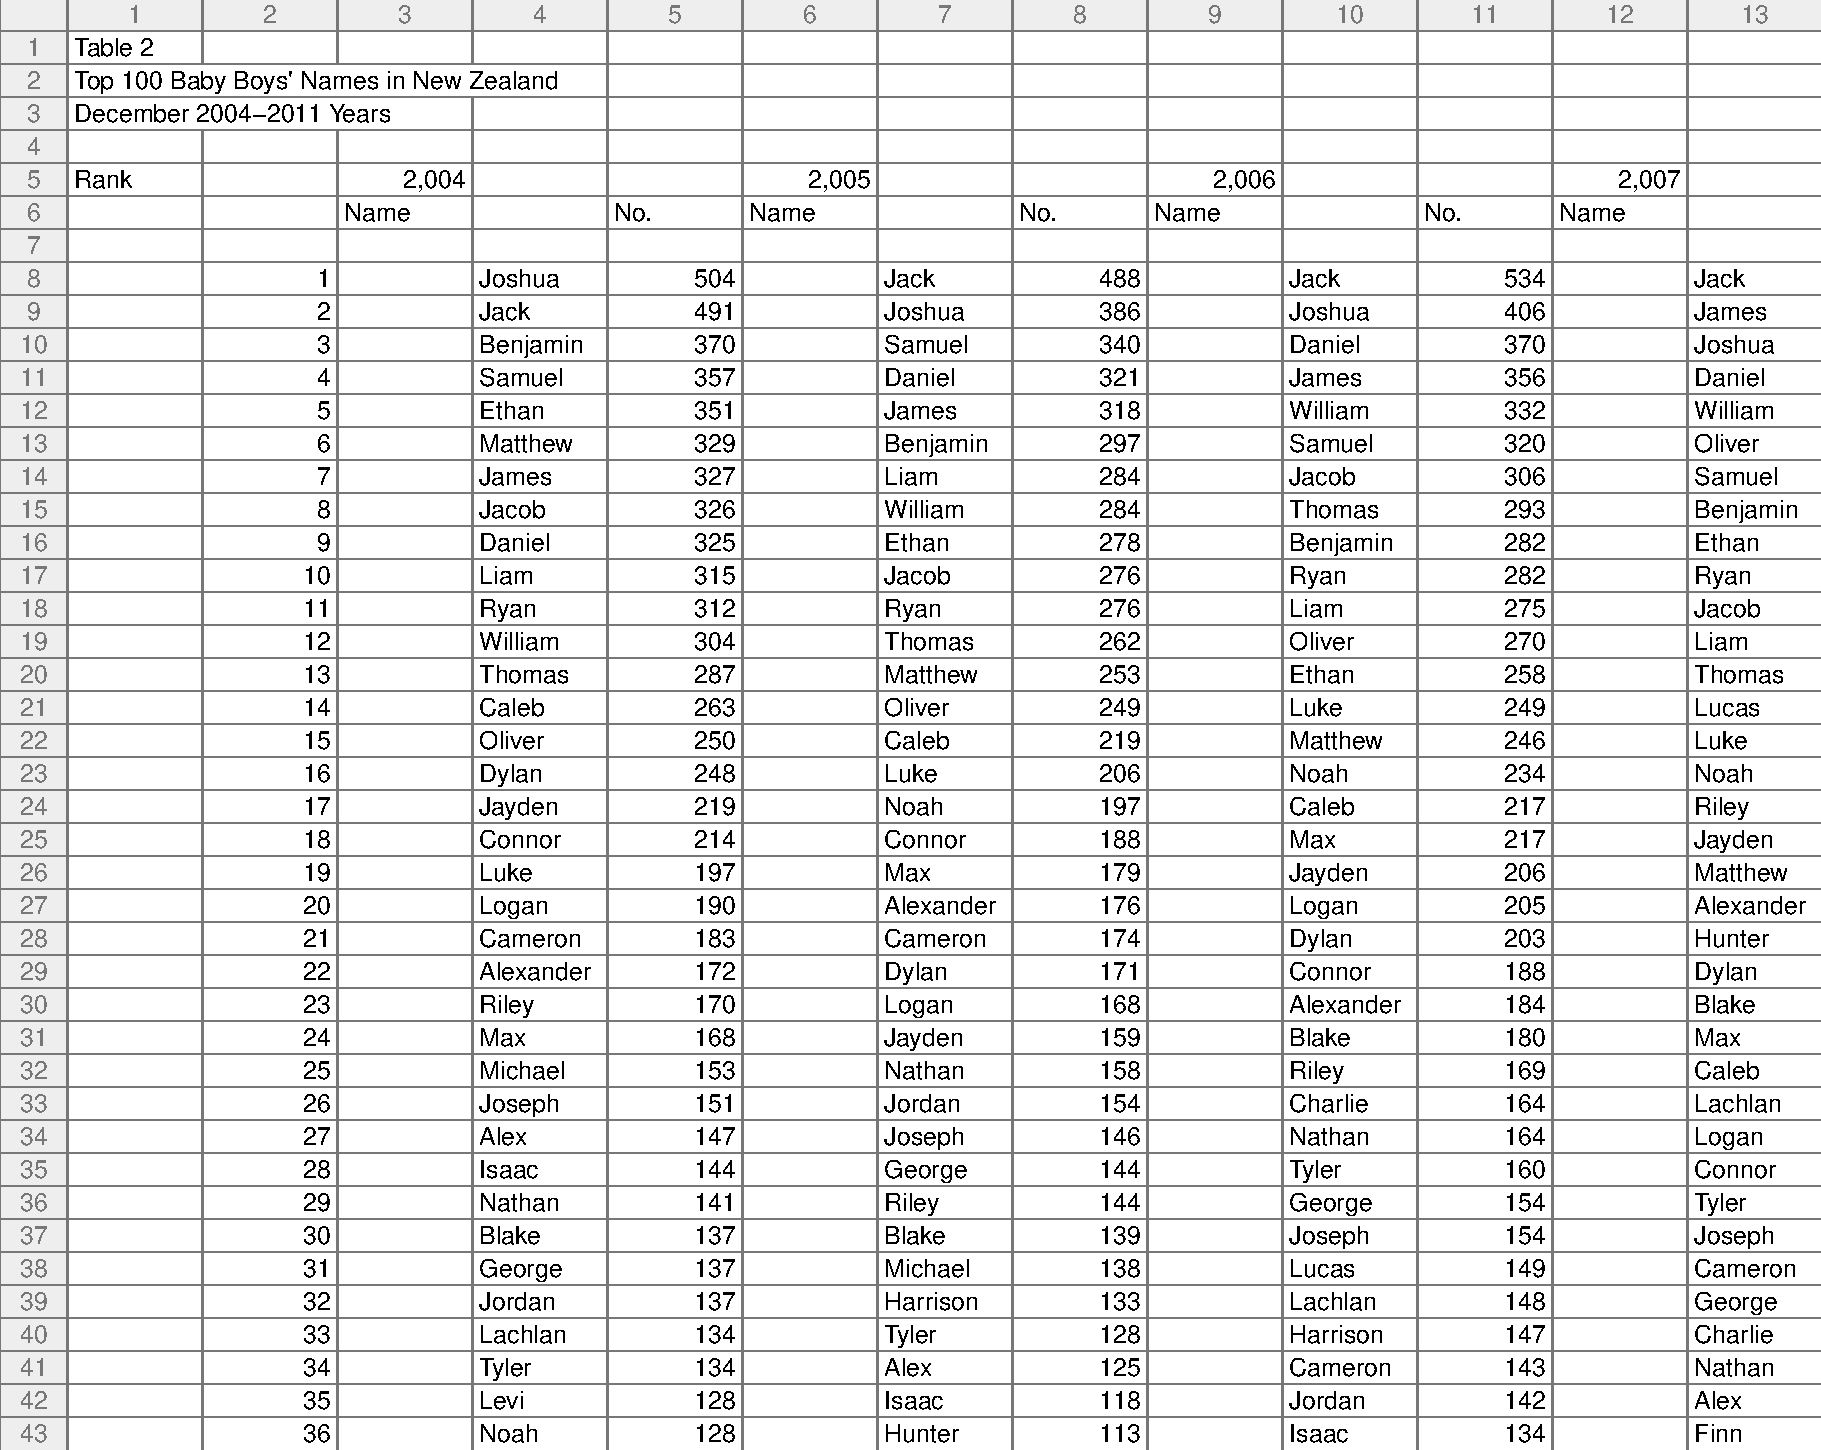
\includegraphics[width=\textwidth]{./TestCase/DIATop100BabyBoysNames2011.pdf}
\end{figure}
\begin{verbatim}
> rowData 
[1]   8 107
> colData 
[1]  2 26
> rowslist 
$label
[1] 1 2 3 5 6

$data
  [1]   8   9  10  11  12  13  14  15  16  17  18  19  20  21  22  23  24  25
 [19]  26  27  28  29  30  31  32  33  34  35  36  37  38  39  40  41  42  43
 [37]  44  45  46  47  48  49  50  51  52  53  54  55  56  57  58  59  60  61
 [55]  62  63  64  65  66  67  68  69  70  71  72  73  74  75  76  77  78  79
 [73]  80  81  82  83  84  85  86  87  88  89  90  91  92  93  94  95  96  97
 [91]  98  99 100 101 102 103 104 105 106 107

> colslist 
$label
[1] 1

$data
 [1]  2  3  4  5  6  7  8  9 10 11 12 13 14 15 16 17 18 19 20 21 22 23 24 25 26

> plist 
$rows
  [1]   1   2   3   4   5   6   7   8   9  10  11  12  13  14  15  16  17  18
 [19]  19  20  21  22  23  24  25  26  27  28  29  30  31  32  33  34  35  36
 [37]  37  38  39  40  41  42  43  44  45  46  47  48  49  50  51  52  53  54
 [55]  55  56  57  58  59  60  61  62  63  64  65  66  67  68  69  70  71  72
 [73]  73  74  75  76  77  78  79  80  81  82  83  84  85  86  87  88  89  90
 [91]  91  92  93  94  95  96  97  98  99 100

$cols
[1] 1

> res 
  1   2   3   4   5   6 
  1   2   3   4   5   6 
> rowplist 
  1   2   3   4   5   6 
  1   2   3   4   5   6 
> rowvecs 
     [,1] 
[1,] "  1"
[2,] "  2"
[3,] "  3"
[4,] "  4"
[5,] "  5"
[6,] "  6"
> matColLabel 
     V3     V5    V6     V8    V9     V11  
[1,] NA     NA    NA     NA    NA     NA   
[2,] NA     NA    NA     NA    NA     NA   
[3,] NA     NA    NA     NA    NA     NA   
[4,] "2004" NA    "2005" NA    "2006" NA   
[5,] "Name" "No." "Name" "No." "Name" "No."
> cursub 
    V3     V5 
"2004"     NA 
> currow[curcols] 
    V3     V5 
"2004"     NA 
> cursub 
    V6     V8 
"2005"     NA 
> currow[curcols] 
    V6     V8 
"2005"     NA 
> cursub 
    V9    V11 
"2006"     NA 
> currow[curcols] 
    V9    V11 
"2006"     NA 
> cursub 
   V12    V14 
"2007"     NA 
> currow[curcols] 
   V12    V14 
"2007"     NA 
> cursub 
   V15    V17 
"2008"     NA 
> currow[curcols] 
   V15    V17 
"2008"     NA 
> cursub 
   V18    V20 
"2009"     NA 
> currow[curcols] 
   V18    V20 
"2009"     NA 
> cursub 
   V21    V23 
"2010"     NA 
> currow[curcols] 
   V21    V23 
"2010"     NA 
> cursub 
   V24    V26 
"2011"     NA 
> currow[curcols] 
   V24    V26 
"2011"     NA 
> cursub 
    V3     V5 
"Name"  "No." 
> currow[curcols] 
    V3     V5 
"Name"  "No." 
> cursub 
    V6     V8 
"Name"  "No." 
> currow[curcols] 
    V6     V8 
"Name"  "No." 
> cursub 
    V9    V11 
"Name"  "No." 
> currow[curcols] 
    V9    V11 
"Name"  "No." 
> cursub 
   V12    V14 
"Name"  "No." 
> currow[curcols] 
   V12    V14 
"Name"  "No." 
> cursub 
   V15    V17 
"Name"  "No." 
> currow[curcols] 
   V15    V17 
"Name"  "No." 
> cursub 
   V18    V20 
"Name"  "No." 
> currow[curcols] 
   V18    V20 
"Name"  "No." 
> cursub 
   V21    V23 
"Name"  "No." 
> currow[curcols] 
   V21    V23 
"Name"  "No." 
> cursub 
   V24    V26 
"Name"  "No." 
> currow[curcols] 
   V24    V26 
"Name"  "No." 
> matColLabel 
     V3     V5    V6     V8    V9     V11  
[1,] NA     NA    NA     NA    NA     NA   
[2,] NA     NA    NA     NA    NA     NA   
[3,] NA     NA    NA     NA    NA     NA   
[4,] "2004" NA    "2005" NA    "2006" NA   
[5,] "Name" "No." "Name" "No." "Name" "No."
> matColLabel 
     V3     V5    V6     V8    V9     V11  
[1,] NA     NA    NA     NA    NA     NA   
[2,] NA     NA    NA     NA    NA     NA   
[3,] NA     NA    NA     NA    NA     NA   
[4,] "2004" NA    "2005" NA    "2006" NA   
[5,] "Name" "No." "Name" "No." "Name" "No."
> matColLabel 
     V3     V5    V6     V8    V9     V11  
[1,] NA     NA    NA     NA    NA     NA   
[2,] NA     NA    NA     NA    NA     NA   
[3,] NA     NA    NA     NA    NA     NA   
[4,] "2004" NA    "2005" NA    "2006" NA   
[5,] "Name" "No." "Name" "No." "Name" "No."
> res 
$`2004`
$`2004`$rows
[1] 1 2

$`2004`$cols
[1] 5


$`2005`
$`2005`$rows
[1] 3 4

$`2005`$cols
[1] 5


$`2006`
$`2006`$rows
[1] 5 6

$`2006`$cols
[1] 5


$`2007`
$`2007`$rows
[1] 7 8

$`2007`$cols
[1] 5


$`2008`
$`2008`$rows
[1]  9 10

$`2008`$cols
[1] 5


$`2009`
$`2009`$rows
[1] 11 12

$`2009`$cols
[1] 5


> plist 
$rows
[1] 1 2

$cols
[1] 5

> res 
Name  No. 
   1    2 
> plist 
$rows
[1] 3 4

$cols
[1] 5

> res 
Name  No. 
   3    4 
> plist 
$rows
[1] 5 6

$cols
[1] 5

> res 
Name  No. 
   5    6 
> plist 
$rows
[1] 7 8

$cols
[1] 5

> res 
Name  No. 
   7    8 
> plist 
$rows
[1]  9 10

$cols
[1] 5

> res 
Name  No. 
   9   10 
> plist 
$rows
[1] 11 12

$cols
[1] 5

> res 
Name  No. 
  11   12 
> plist 
$rows
[1] 13 14

$cols
[1] 5

> res 
Name  No. 
  13   14 
> plist 
$rows
[1] 15 16

$cols
[1] 5

> res 
Name  No. 
  15   16 
> plist 
Name  No. 
   1    2 
> matData 
     V4         V5    V7         V8    V10       V11  
[1,] "Joshua"   "504" "Jack"     "488" "Jack"    "534"
[2,] "Jack"     "491" "Joshua"   "386" "Joshua"  "406"
[3,] "Benjamin" "370" "Samuel"   "340" "Daniel"  "370"
[4,] "Samuel"   "357" "Daniel"   "321" "James"   "356"
[5,] "Ethan"    "351" "James"    "318" "William" "332"
[6,] "Matthew"  "329" "Benjamin" "297" "Samuel"  "320"
> datbit 
     V4         V5   
[1,] "Joshua"   "504"
[2,] "Jack"     "491"
[3,] "Benjamin" "370"
[4,] "Samuel"   "357"
[5,] "Ethan"    "351"
[6,] "Matthew"  "329"
> plist 
Name  No. 
   3    4 
> matData 
     V4         V5    V7         V8    V10       V11  
[1,] "Joshua"   "504" "Jack"     "488" "Jack"    "534"
[2,] "Jack"     "491" "Joshua"   "386" "Joshua"  "406"
[3,] "Benjamin" "370" "Samuel"   "340" "Daniel"  "370"
[4,] "Samuel"   "357" "Daniel"   "321" "James"   "356"
[5,] "Ethan"    "351" "James"    "318" "William" "332"
[6,] "Matthew"  "329" "Benjamin" "297" "Samuel"  "320"
> datbit 
     V7         V8   
[1,] "Jack"     "488"
[2,] "Joshua"   "386"
[3,] "Samuel"   "340"
[4,] "Daniel"   "321"
[5,] "James"    "318"
[6,] "Benjamin" "297"
> plist 
Name  No. 
   5    6 
> matData 
     V4         V5    V7         V8    V10       V11  
[1,] "Joshua"   "504" "Jack"     "488" "Jack"    "534"
[2,] "Jack"     "491" "Joshua"   "386" "Joshua"  "406"
[3,] "Benjamin" "370" "Samuel"   "340" "Daniel"  "370"
[4,] "Samuel"   "357" "Daniel"   "321" "James"   "356"
[5,] "Ethan"    "351" "James"    "318" "William" "332"
[6,] "Matthew"  "329" "Benjamin" "297" "Samuel"  "320"
> datbit 
     V10       V11  
[1,] "Jack"    "534"
[2,] "Joshua"  "406"
[3,] "Daniel"  "370"
[4,] "James"   "356"
[5,] "William" "332"
[6,] "Samuel"  "320"
> plist 
Name  No. 
   7    8 
> matData 
     V4         V5    V7         V8    V10       V11  
[1,] "Joshua"   "504" "Jack"     "488" "Jack"    "534"
[2,] "Jack"     "491" "Joshua"   "386" "Joshua"  "406"
[3,] "Benjamin" "370" "Samuel"   "340" "Daniel"  "370"
[4,] "Samuel"   "357" "Daniel"   "321" "James"   "356"
[5,] "Ethan"    "351" "James"    "318" "William" "332"
[6,] "Matthew"  "329" "Benjamin" "297" "Samuel"  "320"
> datbit 
     V13       V14  
[1,] "Jack"    "499"
[2,] "James"   "369"
[3,] "Joshua"  "366"
[4,] "Daniel"  "351"
[5,] "William" "324"
[6,] "Oliver"  "319"
> plist 
Name  No. 
   9   10 
> matData 
     V4         V5    V7         V8    V10       V11  
[1,] "Joshua"   "504" "Jack"     "488" "Jack"    "534"
[2,] "Jack"     "491" "Joshua"   "386" "Joshua"  "406"
[3,] "Benjamin" "370" "Samuel"   "340" "Daniel"  "370"
[4,] "Samuel"   "357" "Daniel"   "321" "James"   "356"
[5,] "Ethan"    "351" "James"    "318" "William" "332"
[6,] "Matthew"  "329" "Benjamin" "297" "Samuel"  "320"
> datbit 
     V16       V17  
[1,] "Jack"    "449"
[2,] "James"   "378"
[3,] "William" "352"
[4,] "Samuel"  "346"
[5,] "Joshua"  "332"
[6,] "Riley"   "328"
> plist 
Name  No. 
  11   12 
> matData 
     V4         V5    V7         V8    V10       V11  
[1,] "Joshua"   "504" "Jack"     "488" "Jack"    "534"
[2,] "Jack"     "491" "Joshua"   "386" "Joshua"  "406"
[3,] "Benjamin" "370" "Samuel"   "340" "Daniel"  "370"
[4,] "Samuel"   "357" "Daniel"   "321" "James"   "356"
[5,] "Ethan"    "351" "James"    "318" "William" "332"
[6,] "Matthew"  "329" "Benjamin" "297" "Samuel"  "320"
> datbit 
     V19       V20  
[1,] "Jack"    "345"
[2,] "Oliver"  "342"
[3,] "James"   "337"
[4,] "Joshua"  "327"
[5,] "William" "326"
[6,] "Samuel"  "313"
> plist 
Name  No. 
  13   14 
> matData 
     V4         V5    V7         V8    V10       V11  
[1,] "Joshua"   "504" "Jack"     "488" "Jack"    "534"
[2,] "Jack"     "491" "Joshua"   "386" "Joshua"  "406"
[3,] "Benjamin" "370" "Samuel"   "340" "Daniel"  "370"
[4,] "Samuel"   "357" "Daniel"   "321" "James"   "356"
[5,] "Ethan"    "351" "James"    "318" "William" "332"
[6,] "Matthew"  "329" "Benjamin" "297" "Samuel"  "320"
> datbit 
     V22       V23  
[1,] "Liam"    "374"
[2,] "James"   "333"
[3,] "Oliver"  "327"
[4,] "Jack"    "325"
[5,] "William" "320"
[6,] "Joshua"  "298"
> plist 
Name  No. 
  15   16 
> matData 
     V4         V5    V7         V8    V10       V11  
[1,] "Joshua"   "504" "Jack"     "488" "Jack"    "534"
[2,] "Jack"     "491" "Joshua"   "386" "Joshua"  "406"
[3,] "Benjamin" "370" "Samuel"   "340" "Daniel"  "370"
[4,] "Samuel"   "357" "Daniel"   "321" "James"   "356"
[5,] "Ethan"    "351" "James"    "318" "William" "332"
[6,] "Matthew"  "329" "Benjamin" "297" "Samuel"  "320"
> datbit 
     V25       V26  
[1,] "Liam"    "315"
[2,] "Joshua"  "292"
[3,] "Oliver"  "286"
[4,] "Lucas"   "279"
[5,] "William" "272"
[6,] "Noah"    "271"
> colplist 
$`2004`
+ Name (1, 5)
+ No. (2, 5)

$`2005`
+ Name (3, 5)
+ No. (4, 5)

$`2006`
+ Name (5, 5)
+ No. (6, 5)

$`2007`
+ Name (7, 5)
+ No. (8, 5)

$`2008`
+ Name (9, 5)
+ No. (10, 5)

$`2009`
+ Name (11, 5)
+ No. (12, 5)

> res 
  UNKNOWN UNKNOWN     Name No.
1    2004       1   Joshua 504
2    2004       2     Jack 491
3    2004       3 Benjamin 370
4    2004       4   Samuel 357
5    2004       5    Ethan 351
6    2004       6  Matthew 329
\end{verbatim}

\newpage
\subsection{DIATop100BabyGirlsNames2011.xls}
\label{sec:TCRO_DIATop100BabyGirlsNames2011.xls}
\begin{figure}[!h]
\centering
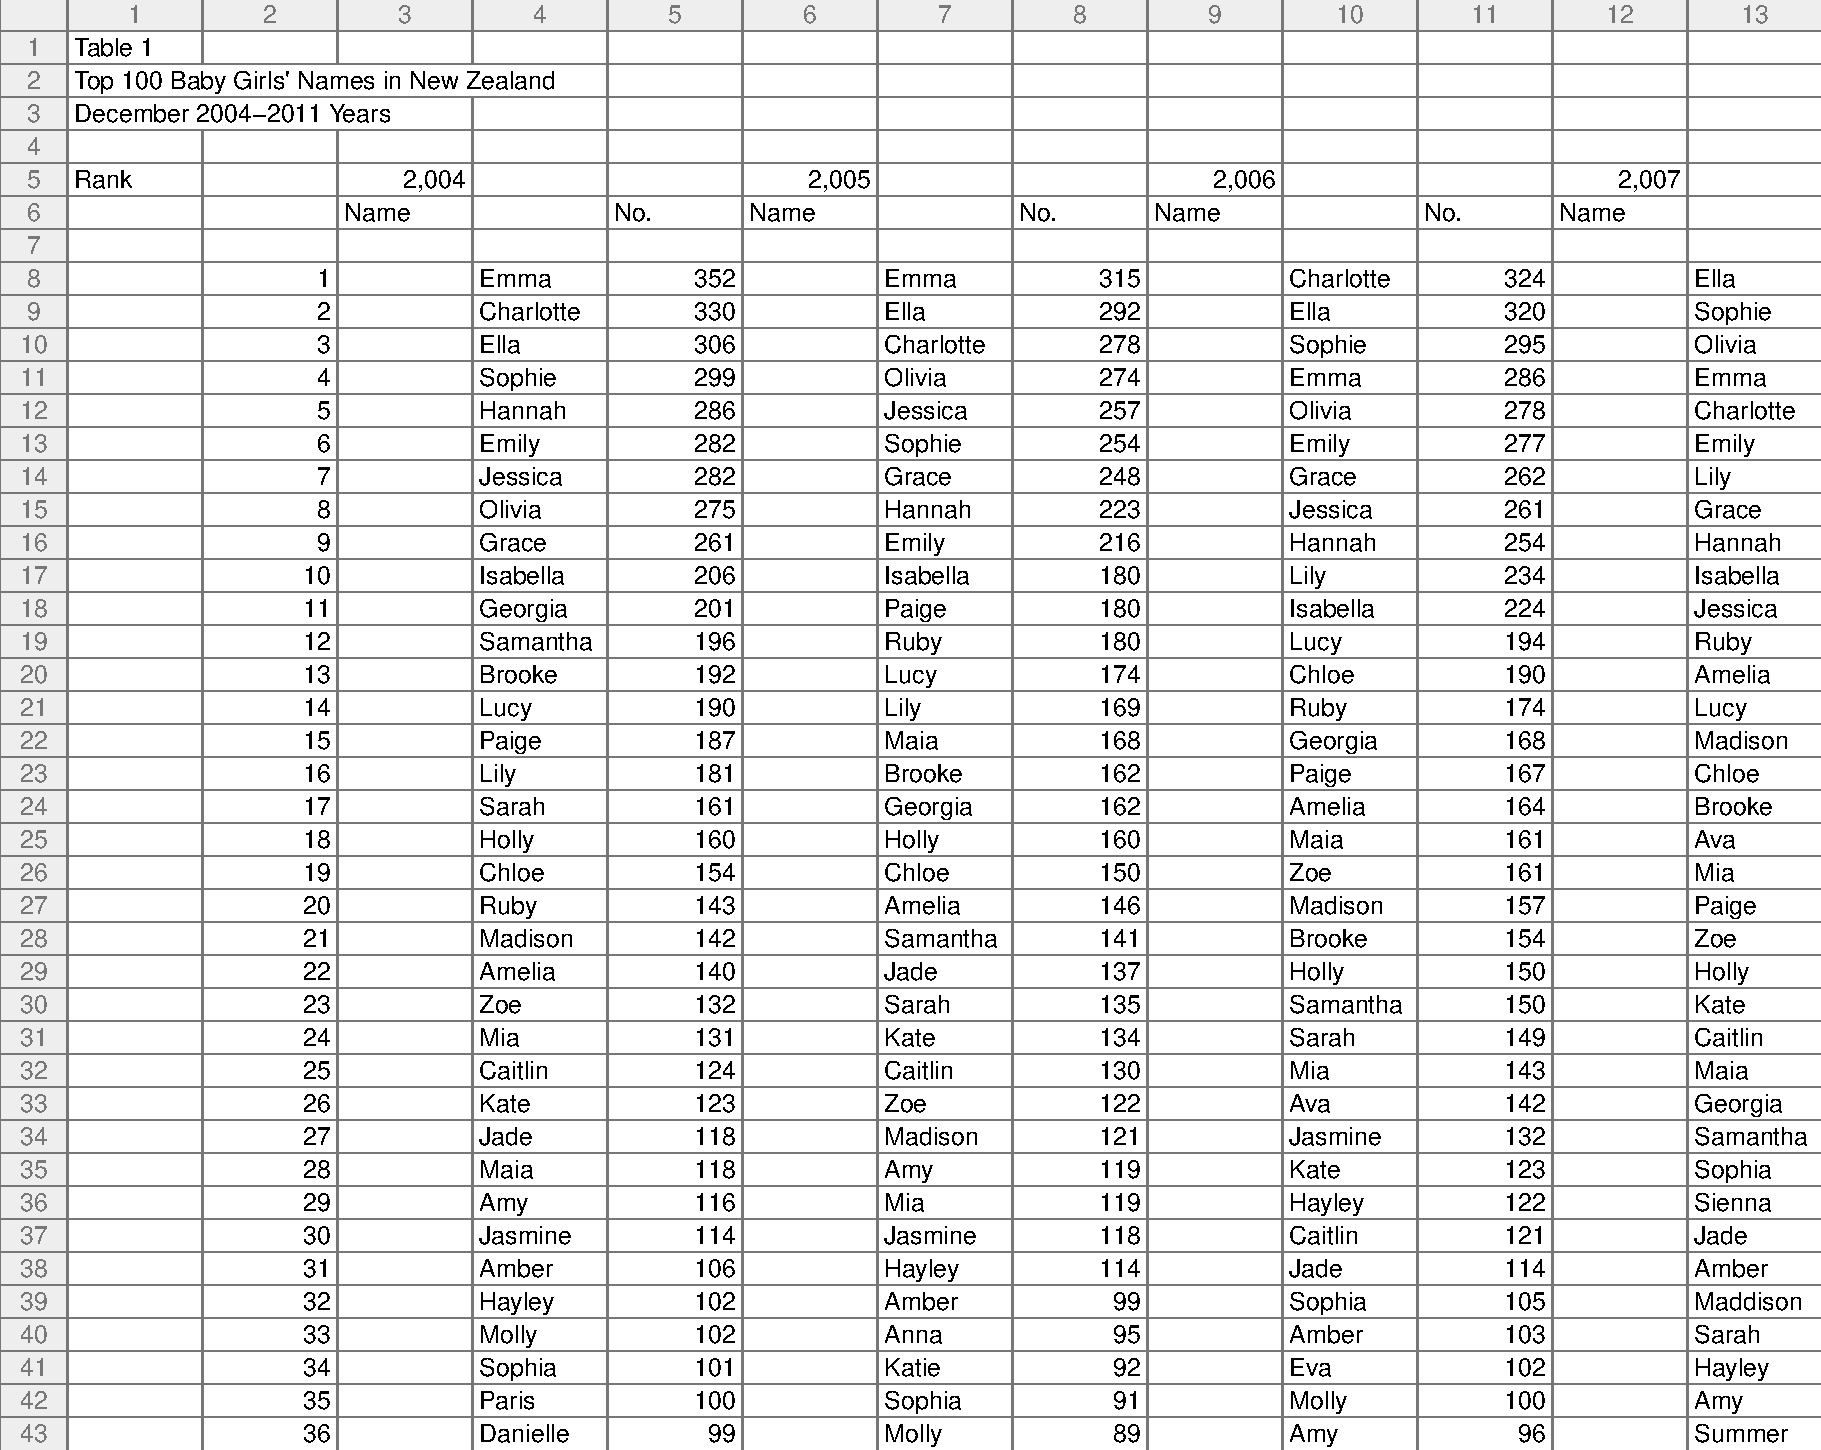
\includegraphics[width=\textwidth]{./TestCase/DIATop100BabyGirlsNames2011.pdf}
\end{figure}
\begin{verbatim}
> rowData 
[1]   8 107
> colData 
[1]  2 26
> rowslist 
$label
[1] 1 2 3 5 6

$data
  [1]   8   9  10  11  12  13  14  15  16  17  18  19  20  21  22  23  24  25
 [19]  26  27  28  29  30  31  32  33  34  35  36  37  38  39  40  41  42  43
 [37]  44  45  46  47  48  49  50  51  52  53  54  55  56  57  58  59  60  61
 [55]  62  63  64  65  66  67  68  69  70  71  72  73  74  75  76  77  78  79
 [73]  80  81  82  83  84  85  86  87  88  89  90  91  92  93  94  95  96  97
 [91]  98  99 100 101 102 103 104 105 106 107

> colslist 
$label
[1] 1

$data
 [1]  2  3  4  5  6  7  8  9 10 11 12 13 14 15 16 17 18 19 20 21 22 23 24 25 26

> plist 
$rows
  [1]   1   2   3   4   5   6   7   8   9  10  11  12  13  14  15  16  17  18
 [19]  19  20  21  22  23  24  25  26  27  28  29  30  31  32  33  34  35  36
 [37]  37  38  39  40  41  42  43  44  45  46  47  48  49  50  51  52  53  54
 [55]  55  56  57  58  59  60  61  62  63  64  65  66  67  68  69  70  71  72
 [73]  73  74  75  76  77  78  79  80  81  82  83  84  85  86  87  88  89  90
 [91]  91  92  93  94  95  96  97  98  99 100

$cols
[1] 1

> res 
  1   2   3   4   5   6 
  1   2   3   4   5   6 
> rowplist 
  1   2   3   4   5   6 
  1   2   3   4   5   6 
> rowvecs 
     [,1] 
[1,] "  1"
[2,] "  2"
[3,] "  3"
[4,] "  4"
[5,] "  5"
[6,] "  6"
> matColLabel 
     V3     V5    V6     V8    V9     V11  
[1,] NA     NA    NA     NA    NA     NA   
[2,] NA     NA    NA     NA    NA     NA   
[3,] NA     NA    NA     NA    NA     NA   
[4,] "2004" NA    "2005" NA    "2006" NA   
[5,] "Name" "No." "Name" "No." "Name" "No."
> cursub 
    V3     V5 
"2004"     NA 
> currow[curcols] 
    V3     V5 
"2004"     NA 
> cursub 
    V6     V8 
"2005"     NA 
> currow[curcols] 
    V6     V8 
"2005"     NA 
> cursub 
    V9    V11 
"2006"     NA 
> currow[curcols] 
    V9    V11 
"2006"     NA 
> cursub 
   V12    V14 
"2007"     NA 
> currow[curcols] 
   V12    V14 
"2007"     NA 
> cursub 
   V15    V17 
"2008"     NA 
> currow[curcols] 
   V15    V17 
"2008"     NA 
> cursub 
   V18    V20 
"2009"     NA 
> currow[curcols] 
   V18    V20 
"2009"     NA 
> cursub 
   V21    V23 
"2010"     NA 
> currow[curcols] 
   V21    V23 
"2010"     NA 
> cursub 
   V24    V26 
"2011"     NA 
> currow[curcols] 
   V24    V26 
"2011"     NA 
> cursub 
    V3     V5 
"Name"  "No." 
> currow[curcols] 
    V3     V5 
"Name"  "No." 
> cursub 
    V6     V8 
"Name"  "No." 
> currow[curcols] 
    V6     V8 
"Name"  "No." 
> cursub 
    V9    V11 
"Name"  "No." 
> currow[curcols] 
    V9    V11 
"Name"  "No." 
> cursub 
   V12    V14 
"Name"  "No." 
> currow[curcols] 
   V12    V14 
"Name"  "No." 
> cursub 
   V15    V17 
"Name"  "No." 
> currow[curcols] 
   V15    V17 
"Name"  "No." 
> cursub 
   V18    V20 
"Name"  "No." 
> currow[curcols] 
   V18    V20 
"Name"  "No." 
> cursub 
   V21    V23 
"Name"  "No." 
> currow[curcols] 
   V21    V23 
"Name"  "No." 
> cursub 
   V24    V26 
"Name"  "No." 
> currow[curcols] 
   V24    V26 
"Name"  "No." 
> matColLabel 
     V3     V5    V6     V8    V9     V11  
[1,] NA     NA    NA     NA    NA     NA   
[2,] NA     NA    NA     NA    NA     NA   
[3,] NA     NA    NA     NA    NA     NA   
[4,] "2004" NA    "2005" NA    "2006" NA   
[5,] "Name" "No." "Name" "No." "Name" "No."
> matColLabel 
     V3     V5    V6     V8    V9     V11  
[1,] NA     NA    NA     NA    NA     NA   
[2,] NA     NA    NA     NA    NA     NA   
[3,] NA     NA    NA     NA    NA     NA   
[4,] "2004" NA    "2005" NA    "2006" NA   
[5,] "Name" "No." "Name" "No." "Name" "No."
> matColLabel 
     V3     V5    V6     V8    V9     V11  
[1,] NA     NA    NA     NA    NA     NA   
[2,] NA     NA    NA     NA    NA     NA   
[3,] NA     NA    NA     NA    NA     NA   
[4,] "2004" NA    "2005" NA    "2006" NA   
[5,] "Name" "No." "Name" "No." "Name" "No."
> res 
$`2004`
$`2004`$rows
[1] 1 2

$`2004`$cols
[1] 5


$`2005`
$`2005`$rows
[1] 3 4

$`2005`$cols
[1] 5


$`2006`
$`2006`$rows
[1] 5 6

$`2006`$cols
[1] 5


$`2007`
$`2007`$rows
[1] 7 8

$`2007`$cols
[1] 5


$`2008`
$`2008`$rows
[1]  9 10

$`2008`$cols
[1] 5


$`2009`
$`2009`$rows
[1] 11 12

$`2009`$cols
[1] 5


> plist 
$rows
[1] 1 2

$cols
[1] 5

> res 
Name  No. 
   1    2 
> plist 
$rows
[1] 3 4

$cols
[1] 5

> res 
Name  No. 
   3    4 
> plist 
$rows
[1] 5 6

$cols
[1] 5

> res 
Name  No. 
   5    6 
> plist 
$rows
[1] 7 8

$cols
[1] 5

> res 
Name  No. 
   7    8 
> plist 
$rows
[1]  9 10

$cols
[1] 5

> res 
Name  No. 
   9   10 
> plist 
$rows
[1] 11 12

$cols
[1] 5

> res 
Name  No. 
  11   12 
> plist 
$rows
[1] 13 14

$cols
[1] 5

> res 
Name  No. 
  13   14 
> plist 
$rows
[1] 15 16

$cols
[1] 5

> res 
Name  No. 
  15   16 
> plist 
Name  No. 
   1    2 
> matData 
     V4          V5    V7          V8    V10         V11  
[1,] "Emma"      "352" "Emma"      "315" "Charlotte" "324"
[2,] "Charlotte" "330" "Ella"      "292" "Ella"      "320"
[3,] "Ella"      "306" "Charlotte" "278" "Sophie"    "295"
[4,] "Sophie"    "299" "Olivia"    "274" "Emma"      "286"
[5,] "Hannah"    "286" "Jessica"   "257" "Olivia"    "278"
[6,] "Emily"     "282" "Sophie"    "254" "Emily"     "277"
> datbit 
     V4          V5   
[1,] "Emma"      "352"
[2,] "Charlotte" "330"
[3,] "Ella"      "306"
[4,] "Sophie"    "299"
[5,] "Hannah"    "286"
[6,] "Emily"     "282"
> plist 
Name  No. 
   3    4 
> matData 
     V4          V5    V7          V8    V10         V11  
[1,] "Emma"      "352" "Emma"      "315" "Charlotte" "324"
[2,] "Charlotte" "330" "Ella"      "292" "Ella"      "320"
[3,] "Ella"      "306" "Charlotte" "278" "Sophie"    "295"
[4,] "Sophie"    "299" "Olivia"    "274" "Emma"      "286"
[5,] "Hannah"    "286" "Jessica"   "257" "Olivia"    "278"
[6,] "Emily"     "282" "Sophie"    "254" "Emily"     "277"
> datbit 
     V7          V8   
[1,] "Emma"      "315"
[2,] "Ella"      "292"
[3,] "Charlotte" "278"
[4,] "Olivia"    "274"
[5,] "Jessica"   "257"
[6,] "Sophie"    "254"
> plist 
Name  No. 
   5    6 
> matData 
     V4          V5    V7          V8    V10         V11  
[1,] "Emma"      "352" "Emma"      "315" "Charlotte" "324"
[2,] "Charlotte" "330" "Ella"      "292" "Ella"      "320"
[3,] "Ella"      "306" "Charlotte" "278" "Sophie"    "295"
[4,] "Sophie"    "299" "Olivia"    "274" "Emma"      "286"
[5,] "Hannah"    "286" "Jessica"   "257" "Olivia"    "278"
[6,] "Emily"     "282" "Sophie"    "254" "Emily"     "277"
> datbit 
     V10         V11  
[1,] "Charlotte" "324"
[2,] "Ella"      "320"
[3,] "Sophie"    "295"
[4,] "Emma"      "286"
[5,] "Olivia"    "278"
[6,] "Emily"     "277"
> plist 
Name  No. 
   7    8 
> matData 
     V4          V5    V7          V8    V10         V11  
[1,] "Emma"      "352" "Emma"      "315" "Charlotte" "324"
[2,] "Charlotte" "330" "Ella"      "292" "Ella"      "320"
[3,] "Ella"      "306" "Charlotte" "278" "Sophie"    "295"
[4,] "Sophie"    "299" "Olivia"    "274" "Emma"      "286"
[5,] "Hannah"    "286" "Jessica"   "257" "Olivia"    "278"
[6,] "Emily"     "282" "Sophie"    "254" "Emily"     "277"
> datbit 
     V13         V14  
[1,] "Ella"      "418"
[2,] "Sophie"    "351"
[3,] "Olivia"    "285"
[4,] "Emma"      "280"
[5,] "Charlotte" "263"
[6,] "Emily"     "258"
> plist 
Name  No. 
   9   10 
> matData 
     V4          V5    V7          V8    V10         V11  
[1,] "Emma"      "352" "Emma"      "315" "Charlotte" "324"
[2,] "Charlotte" "330" "Ella"      "292" "Ella"      "320"
[3,] "Ella"      "306" "Charlotte" "278" "Sophie"    "295"
[4,] "Sophie"    "299" "Olivia"    "274" "Emma"      "286"
[5,] "Hannah"    "286" "Jessica"   "257" "Olivia"    "278"
[6,] "Emily"     "282" "Sophie"    "254" "Emily"     "277"
> datbit 
     V16         V17  
[1,] "Sophie"    "356"
[2,] "Olivia"    "308"
[3,] "Ella"      "297"
[4,] "Isabella"  "288"
[5,] "Charlotte" "269"
[6,] "Lily"      "254"
> plist 
Name  No. 
  11   12 
> matData 
     V4          V5    V7          V8    V10         V11  
[1,] "Emma"      "352" "Emma"      "315" "Charlotte" "324"
[2,] "Charlotte" "330" "Ella"      "292" "Ella"      "320"
[3,] "Ella"      "306" "Charlotte" "278" "Sophie"    "295"
[4,] "Sophie"    "299" "Olivia"    "274" "Emma"      "286"
[5,] "Hannah"    "286" "Jessica"   "257" "Olivia"    "278"
[6,] "Emily"     "282" "Sophie"    "254" "Emily"     "277"
> datbit 
     V19        V20  
[1,] "Sophie"   "386"
[2,] "Ruby"     "305"
[3,] "Olivia"   "304"
[4,] "Isabella" "288"
[5,] "Ella"     "283"
[6,] "Emily"    "266"
> plist 
Name  No. 
  13   14 
> matData 
     V4          V5    V7          V8    V10         V11  
[1,] "Emma"      "352" "Emma"      "315" "Charlotte" "324"
[2,] "Charlotte" "330" "Ella"      "292" "Ella"      "320"
[3,] "Ella"      "306" "Charlotte" "278" "Sophie"    "295"
[4,] "Sophie"    "299" "Olivia"    "274" "Emma"      "286"
[5,] "Hannah"    "286" "Jessica"   "257" "Olivia"    "278"
[6,] "Emily"     "282" "Sophie"    "254" "Emily"     "277"
> datbit 
     V22         V23  
[1,] "Sophie"    "377"
[2,] "Olivia"    "335"
[3,] "Ruby"      "322"
[4,] "Charlotte" "305"
[5,] "Isabella"  "286"
[6,] "Lily"      "281"
> plist 
Name  No. 
  15   16 
> matData 
     V4          V5    V7          V8    V10         V11  
[1,] "Emma"      "352" "Emma"      "315" "Charlotte" "324"
[2,] "Charlotte" "330" "Ella"      "292" "Ella"      "320"
[3,] "Ella"      "306" "Charlotte" "278" "Sophie"    "295"
[4,] "Sophie"    "299" "Olivia"    "274" "Emma"      "286"
[5,] "Hannah"    "286" "Jessica"   "257" "Olivia"    "278"
[6,] "Emily"     "282" "Sophie"    "254" "Emily"     "277"
> datbit 
     V25         V26  
[1,] "Ruby"      "335"
[2,] "Olivia"    "324"
[3,] "Sophie"    "309"
[4,] "Isabella"  "277"
[5,] "Charlotte" "258"
[6,] "Grace"     "246"
> colplist 
$`2004`
+ Name (1, 5)
+ No. (2, 5)

$`2005`
+ Name (3, 5)
+ No. (4, 5)

$`2006`
+ Name (5, 5)
+ No. (6, 5)

$`2007`
+ Name (7, 5)
+ No. (8, 5)

$`2008`
+ Name (9, 5)
+ No. (10, 5)

$`2009`
+ Name (11, 5)
+ No. (12, 5)

> res 
  UNKNOWN UNKNOWN      Name No.
1    2004       1      Emma 352
2    2004       2 Charlotte 330
3    2004       3      Ella 306
4    2004       4    Sophie 299
5    2004       5    Hannah 286
6    2004       6     Emily 282
\end{verbatim}

\newpage
\subsection{NZQAScholarships.xls}
\label{sec:TCRO_NZQAScholarships.xls}
\begin{figure}[!h]
\centering
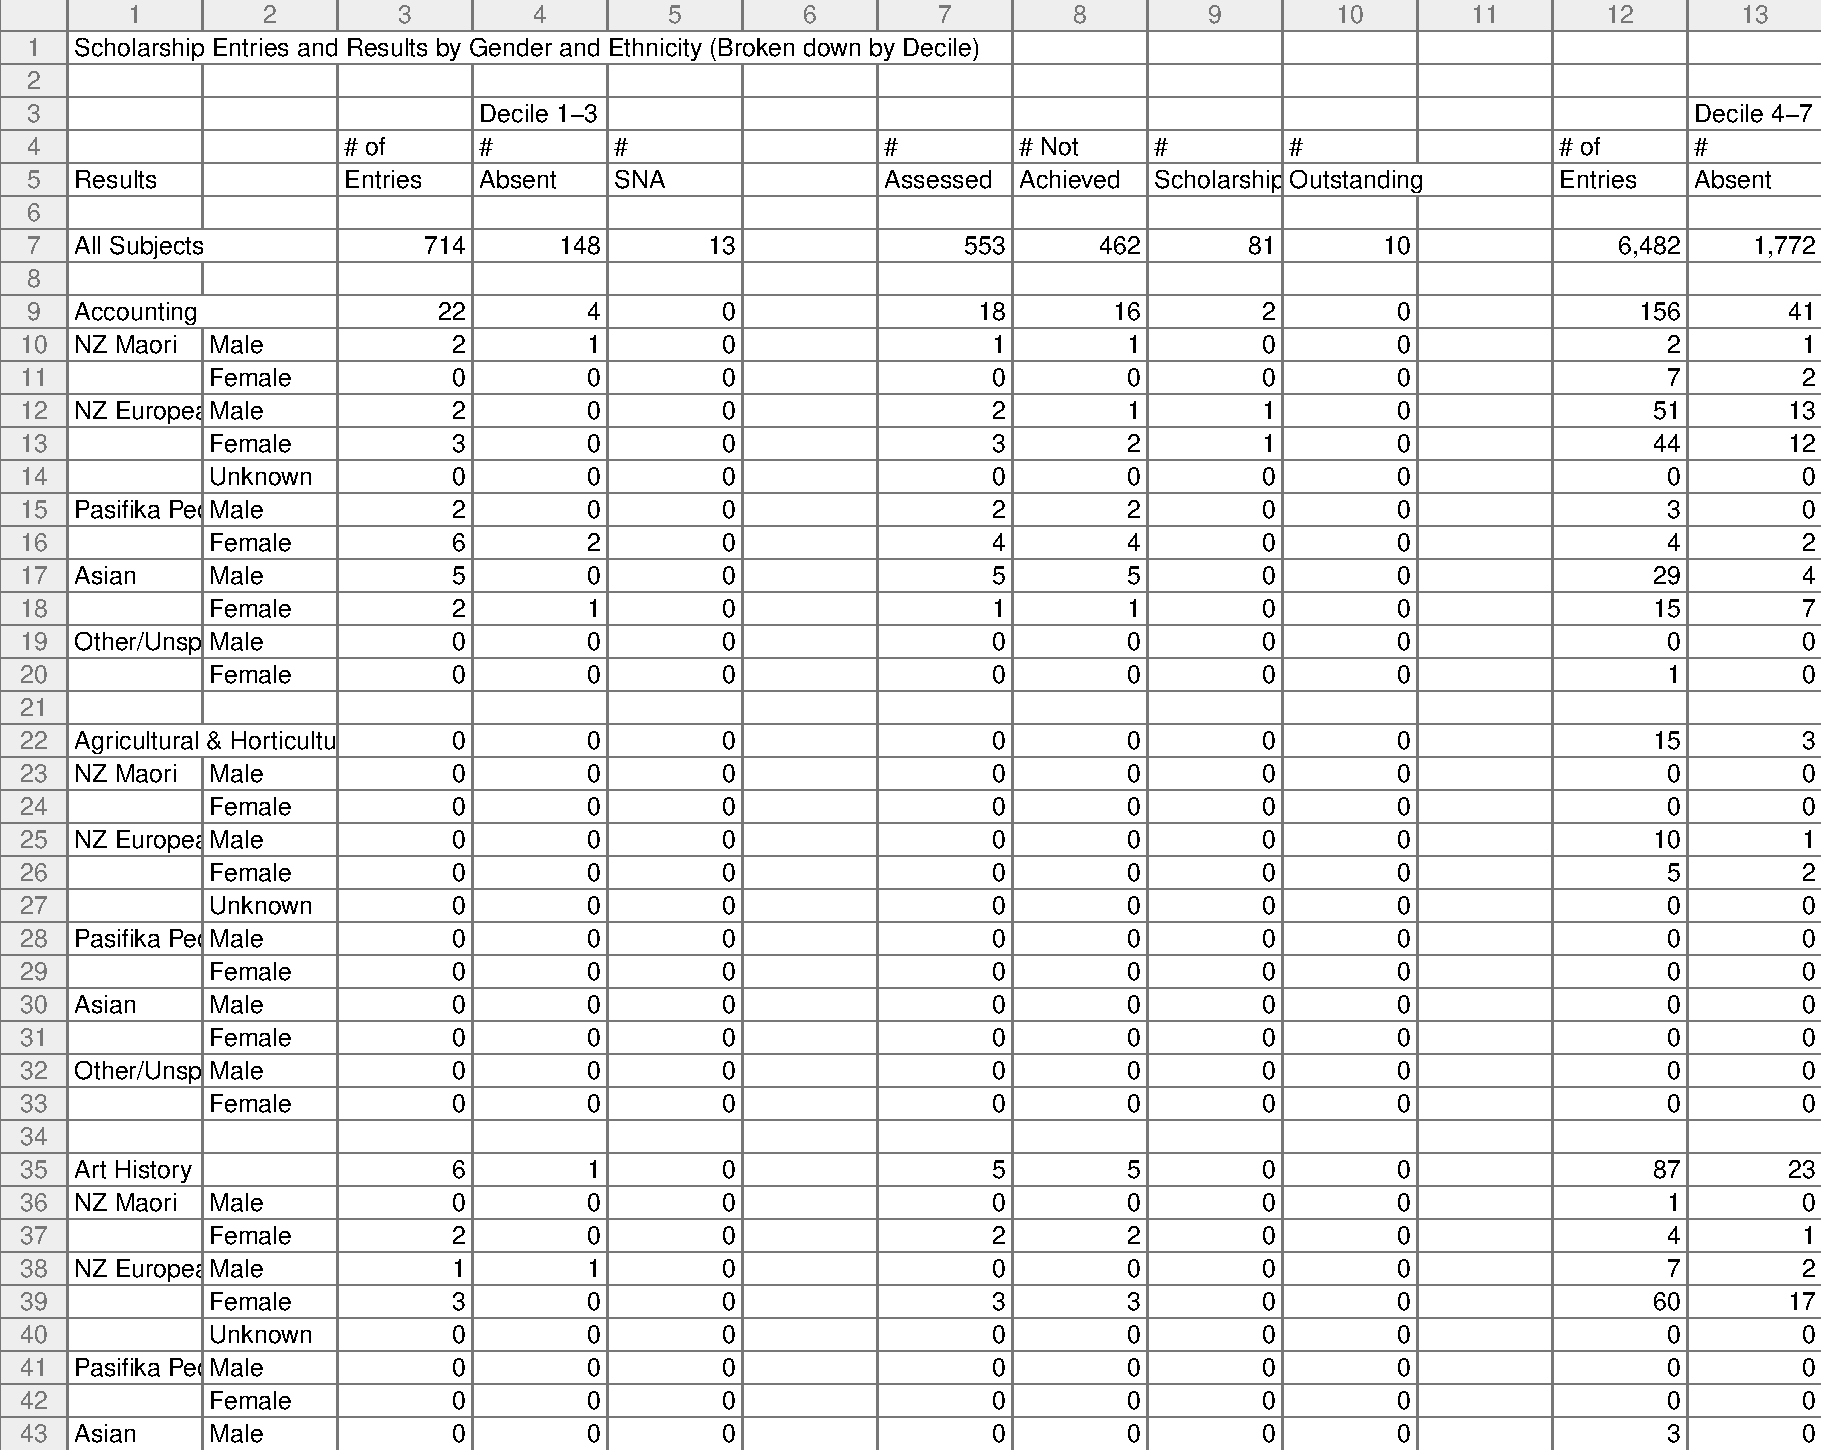
\includegraphics[width=\textwidth]{./TestCase/NZQAScholarships.pdf}
\end{figure}
\begin{verbatim}
> rowData 
[1]   7 462
> colData 
[1]  3 28
> rowslist 
$label
[1] 1 3 4 5

$data
  [1]   7   9  10  11  12  13  14  15  16  17  18  19  20  22  23  24  25  26
 [19]  27  28  29  30  31  32  33  35  36  37  38  39  40  41  42  43  44  45
 [37]  46  48  49  50  51  52  53  54  55  56  57  58  59  61  62  63  64  65
 [55]  66  67  68  69  70  71  72  74  75  76  77  78  79  80  81  82  83  84
 [73]  85  87  88  89  90  91  92  93  94  95  96  97  98 100 101 102 103 104
 [91] 105 106 107 108 109 110 111 113 114 115 116 117 118 119 120 121 122 123
[109] 124 126 127 128 129 130 131 132 133 134 135 136 137 139 140 141 142 143
[127] 144 145 146 147 148 149 150 152 153 154 155 156 157 158 159 160 161 162
[145] 163 165 166 167 168 169 170 171 172 173 174 175 176 178 179 180 181 182
[163] 183 184 185 186 187 188 189 191 192 193 194 195 196 197 198 199 200 201
[181] 202 204 205 206 207 208 209 210 211 212 213 214 215 217 218 219 220 221
[199] 222 223 224 225 226 227 228 230 231 232 233 234 235 236 237 238 239 240
[217] 241 243 244 245 246 247 248 249 250 251 252 253 254 256 257 258 259 260
[235] 261 262 263 264 265 266 267 269 270 271 272 273 274 275 276 277 278 279
[253] 280 282 283 284 285 286 287 288 289 290 291 292 293 295 296 297 298 299
[271] 300 301 302 303 304 305 306 308 309 310 311 312 313 314 315 316 317 318
[289] 319 321 322 323 324 325 326 327 328 329 330 331 332 334 335 336 337 338
[307] 339 340 341 342 343 344 345 347 348 349 350 351 352 353 354 355 356 357
[325] 358 360 361 362 363 364 365 366 367 368 369 370 371 373 374 375 376 377
[343] 378 379 380 381 382 383 384 386 387 388 389 390 391 392 393 394 395 396
[361] 397 399 400 401 402 403 404 405 406 407 408 409 410 412 413 414 415 416
[379] 417 418 419 420 421 422 423 425 426 427 428 429 430 431 432 433 434 435
[397] 436 438 439 440 441 442 443 444 445 446 447 448 449 451 452 453 454 455
[415] 456 457 458 459 460 461 462

> colslist 
$label
[1] 1 2

$data
 [1]  3  4  5  7  8  9 10 12 13 14 16 17 18 19 21 22 23 25 26 27 28

> res 
$`All Subjects`
$`All Subjects`$rows
  [1]   2   3   4   5   6   7   8   9  10  11  12  13  14  15  16  17  18  19
 [19]  20  21  22  23  24  25  26  27  28  29  30  31  32  33  34  35  36  37
 [37]  38  39  40  41  42  43  44  45  46  47  48  49  50  51  52  53  54  55
 [55]  56  57  58  59  60  61  62  63  64  65  66  67  68  69  70  71  72  73
 [73]  74  75  76  77  78  79  80  81  82  83  84  85  86  87  88  89  90  91
 [91]  92  93  94  95  96  97  98  99 100 101 102 103 104 105 106 107 108 109
[109] 110 111 112 113 114 115 116 117 118 119 120 121 122 123 124 125 126 127
[127] 128 129 130 131 132 133 134 135 136 137 138 139 140 141 142 143 144 145
[145] 146 147 148 149 150 151 152 153 154 155 156 157 158 159 160 161 162 163
[163] 164 165 166 167 168 169 170 171 172 173 174 175 176 177 178 179 180 181
[181] 182 183 184 185 186 187 188 189 190 191 192 193 194 195 196 197 198 199
[199] 200 201 202 203 204 205 206 207 208 209 210 211 212 213 214 215 216 217
[217] 218 219 220 221 222 223 224 225 226 227 228 229 230 231 232 233 234 235
[235] 236 237 238 239 240 241 242 243 244 245 246 247 248 249 250 251 252 253
[253] 254 255 256 257 258 259 260 261 262 263 264 265 266 267 268 269 270 271
[271] 272 273 274 275 276 277 278 279 280 281 282 283 284 285 286 287 288 289
[289] 290 291 292 293 294 295 296 297 298 299 300 301 302 303 304 305 306 307
[307] 308 309 310 311 312 313 314 315 316 317 318 319 320 321 322 323 324 325
[325] 326 327 328 329 330 331 332 333 334 335 336 337 338 339 340 341 342 343
[343] 344 345 346 347 348 349 350 351 352 353 354 355 356 357 358 359 360 361
[361] 362 363 364 365 366 367 368 369 370 371 372 373 374 375 376 377 378 379
[379] 380 381 382 383 384 385 386 387 388 389 390 391 392 393 394 395 396 397
[397] 398 399 400 401 402 403 404 405 406 407 408 409 410 411 412 413 414 415
[415] 416 417 418 419 420 421

$`All Subjects`$cols
[1] 1 2


> res 
$Accounting
$Accounting$rows
 [1]  3  4  5  6  7  8  9 10 11 12 13

$Accounting$cols
[1] 1 2


$`Agricultural & Horticultural Science`
$`Agricultural & Horticultural Science`$rows
 [1] 15 16 17 18 19 20 21 22 23 24 25

$`Agricultural & Horticultural Science`$cols
[1] 1 2


$`Art History`
$`Art History`$rows
 [1] 27 28 29 30 31 32 33 34 35 36 37

$`Art History`$cols
[1] 1 2


$Biology
$Biology$rows
 [1] 39 40 41 42 43 44 45 46 47 48 49

$Biology$cols
[1] 1 2


$Chemistry
$Chemistry$rows
 [1] 51 52 53 54 55 56 57 58 59 60 61

$Chemistry$cols
[1] 1 2


$Chinese
$Chinese$rows
 [1] 63 64 65 66 67 68 69 70 71 72 73

$Chinese$cols
[1] 1 2


> res 
$`NZ Maori`
$`NZ Maori`$rows
[1] 3 4

$`NZ Maori`$cols
[1] 2


$`NZ European`
$`NZ European`$rows
[1] 5 6 7

$`NZ European`$cols
[1] 2


$`Pasifika Peoples`
$`Pasifika Peoples`$rows
[1] 8 9

$`Pasifika Peoples`$cols
[1] 2


$Asian
$Asian$rows
[1] 10 11

$Asian$cols
[1] 2


$`Other/Unspecified Ethnicity`
$`Other/Unspecified Ethnicity`$rows
[1] 12 13

$`Other/Unspecified Ethnicity`$cols
[1] 2


> plist 
$rows
[1] 3 4

$cols
[1] 2

> res 
  Male Female 
     3      4 
> plist 
$rows
[1] 5 6 7

$cols
[1] 2

> res 
   Male  Female Unknown 
      5       6       7 
> plist 
$rows
[1] 8 9

$cols
[1] 2

> res 
  Male Female 
     8      9 
> plist 
$rows
[1] 10 11

$cols
[1] 2

> res 
  Male Female 
    10     11 
> plist 
$rows
[1] 12 13

$cols
[1] 2

> res 
  Male Female 
    12     13 
> res 
$`NZ Maori`
$`NZ Maori`$rows
[1] 15 16

$`NZ Maori`$cols
[1] 2


$`NZ European`
$`NZ European`$rows
[1] 17 18 19

$`NZ European`$cols
[1] 2


$`Pasifika Peoples`
$`Pasifika Peoples`$rows
[1] 20 21

$`Pasifika Peoples`$cols
[1] 2


$Asian
$Asian$rows
[1] 22 23

$Asian$cols
[1] 2


$`Other/Unspecified Ethnicity`
$`Other/Unspecified Ethnicity`$rows
[1] 24 25

$`Other/Unspecified Ethnicity`$cols
[1] 2


> plist 
$rows
[1] 15 16

$cols
[1] 2

> res 
  Male Female 
    15     16 
> plist 
$rows
[1] 17 18 19

$cols
[1] 2

> res 
   Male  Female Unknown 
     17      18      19 
> plist 
$rows
[1] 20 21

$cols
[1] 2

> res 
  Male Female 
    20     21 
> plist 
$rows
[1] 22 23

$cols
[1] 2

> res 
  Male Female 
    22     23 
> plist 
$rows
[1] 24 25

$cols
[1] 2

> res 
  Male Female 
    24     25 
> res 
$`NZ Maori`
$`NZ Maori`$rows
[1] 27 28

$`NZ Maori`$cols
[1] 2


$`NZ European`
$`NZ European`$rows
[1] 29 30 31

$`NZ European`$cols
[1] 2


$`Pasifika Peoples`
$`Pasifika Peoples`$rows
[1] 32 33

$`Pasifika Peoples`$cols
[1] 2


$Asian
$Asian$rows
[1] 34 35

$Asian$cols
[1] 2


$`Other/Unspecified Ethnicity`
$`Other/Unspecified Ethnicity`$rows
[1] 36 37

$`Other/Unspecified Ethnicity`$cols
[1] 2


> plist 
$rows
[1] 27 28

$cols
[1] 2

> res 
  Male Female 
    27     28 
> plist 
$rows
[1] 29 30 31

$cols
[1] 2

> res 
   Male  Female Unknown 
     29      30      31 
> plist 
$rows
[1] 32 33

$cols
[1] 2

> res 
  Male Female 
    32     33 
> plist 
$rows
[1] 34 35

$cols
[1] 2

> res 
  Male Female 
    34     35 
> plist 
$rows
[1] 36 37

$cols
[1] 2

> res 
  Male Female 
    36     37 
> res 
$`NZ Maori`
$`NZ Maori`$rows
[1] 39 40

$`NZ Maori`$cols
[1] 2


$`NZ European`
$`NZ European`$rows
[1] 41 42 43

$`NZ European`$cols
[1] 2


$`Pasifika Peoples`
$`Pasifika Peoples`$rows
[1] 44 45

$`Pasifika Peoples`$cols
[1] 2


$Asian
$Asian$rows
[1] 46 47

$Asian$cols
[1] 2


$`Other/Unspecified Ethnicity`
$`Other/Unspecified Ethnicity`$rows
[1] 48 49

$`Other/Unspecified Ethnicity`$cols
[1] 2


> plist 
$rows
[1] 39 40

$cols
[1] 2

> res 
  Male Female 
    39     40 
> plist 
$rows
[1] 41 42 43

$cols
[1] 2

> res 
   Male  Female Unknown 
     41      42      43 
> plist 
$rows
[1] 44 45

$cols
[1] 2

> res 
  Male Female 
    44     45 
> plist 
$rows
[1] 46 47

$cols
[1] 2

> res 
  Male Female 
    46     47 
> plist 
$rows
[1] 48 49

$cols
[1] 2

> res 
  Male Female 
    48     49 
> res 
$`NZ Maori`
$`NZ Maori`$rows
[1] 51 52

$`NZ Maori`$cols
[1] 2


$`NZ European`
$`NZ European`$rows
[1] 53 54 55

$`NZ European`$cols
[1] 2


$`Pasifika Peoples`
$`Pasifika Peoples`$rows
[1] 56 57

$`Pasifika Peoples`$cols
[1] 2


$Asian
$Asian$rows
[1] 58 59

$Asian$cols
[1] 2


$`Other/Unspecified Ethnicity`
$`Other/Unspecified Ethnicity`$rows
[1] 60 61

$`Other/Unspecified Ethnicity`$cols
[1] 2


> plist 
$rows
[1] 51 52

$cols
[1] 2

> res 
  Male Female 
    51     52 
> plist 
$rows
[1] 53 54 55

$cols
[1] 2

> res 
   Male  Female Unknown 
     53      54      55 
> plist 
$rows
[1] 56 57

$cols
[1] 2

> res 
  Male Female 
    56     57 
> plist 
$rows
[1] 58 59

$cols
[1] 2

> res 
  Male Female 
    58     59 
> plist 
$rows
[1] 60 61

$cols
[1] 2

> res 
  Male Female 
    60     61 
> res 
$`NZ Maori`
$`NZ Maori`$rows
[1] 63 64

$`NZ Maori`$cols
[1] 2


$`NZ European`
$`NZ European`$rows
[1] 65 66 67

$`NZ European`$cols
[1] 2


$`Pasifika Peoples`
$`Pasifika Peoples`$rows
[1] 68 69

$`Pasifika Peoples`$cols
[1] 2


$Asian
$Asian$rows
[1] 70 71

$Asian$cols
[1] 2


$`Other/Unspecified Ethnicity`
$`Other/Unspecified Ethnicity`$rows
[1] 72 73

$`Other/Unspecified Ethnicity`$cols
[1] 2


> plist 
$rows
[1] 63 64

$cols
[1] 2

> res 
  Male Female 
    63     64 
> plist 
$rows
[1] 65 66 67

$cols
[1] 2

> res 
   Male  Female Unknown 
     65      66      67 
> plist 
$rows
[1] 68 69

$cols
[1] 2

> res 
  Male Female 
    68     69 
> plist 
$rows
[1] 70 71

$cols
[1] 2

> res 
  Male Female 
    70     71 
> plist 
$rows
[1] 72 73

$cols
[1] 2

> res 
  Male Female 
    72     73 
> res 
$`NZ Maori`
$`NZ Maori`$rows
[1] 75 76

$`NZ Maori`$cols
[1] 2


$`NZ European`
$`NZ European`$rows
[1] 77 78 79

$`NZ European`$cols
[1] 2


$`Pasifika Peoples`
$`Pasifika Peoples`$rows
[1] 80 81

$`Pasifika Peoples`$cols
[1] 2


$Asian
$Asian$rows
[1] 82 83

$Asian$cols
[1] 2


$`Other/Unspecified Ethnicity`
$`Other/Unspecified Ethnicity`$rows
[1] 84 85

$`Other/Unspecified Ethnicity`$cols
[1] 2


> plist 
$rows
[1] 75 76

$cols
[1] 2

> res 
  Male Female 
    75     76 
> plist 
$rows
[1] 77 78 79

$cols
[1] 2

> res 
   Male  Female Unknown 
     77      78      79 
> plist 
$rows
[1] 80 81

$cols
[1] 2

> res 
  Male Female 
    80     81 
> plist 
$rows
[1] 82 83

$cols
[1] 2

> res 
  Male Female 
    82     83 
> plist 
$rows
[1] 84 85

$cols
[1] 2

> res 
  Male Female 
    84     85 
> res 
$`NZ Maori`
$`NZ Maori`$rows
[1] 87 88

$`NZ Maori`$cols
[1] 2


$`NZ European`
$`NZ European`$rows
[1] 89 90 91

$`NZ European`$cols
[1] 2


$`Pasifika Peoples`
$`Pasifika Peoples`$rows
[1] 92 93

$`Pasifika Peoples`$cols
[1] 2


$Asian
$Asian$rows
[1] 94 95

$Asian$cols
[1] 2


$`Other/Unspecified Ethnicity`
$`Other/Unspecified Ethnicity`$rows
[1] 96 97

$`Other/Unspecified Ethnicity`$cols
[1] 2


> plist 
$rows
[1] 87 88

$cols
[1] 2

> res 
  Male Female 
    87     88 
> plist 
$rows
[1] 89 90 91

$cols
[1] 2

> res 
   Male  Female Unknown 
     89      90      91 
> plist 
$rows
[1] 92 93

$cols
[1] 2

> res 
  Male Female 
    92     93 
> plist 
$rows
[1] 94 95

$cols
[1] 2

> res 
  Male Female 
    94     95 
> plist 
$rows
[1] 96 97

$cols
[1] 2

> res 
  Male Female 
    96     97 
> res 
$`NZ Maori`
$`NZ Maori`$rows
[1]  99 100

$`NZ Maori`$cols
[1] 2


$`NZ European`
$`NZ European`$rows
[1] 101 102 103

$`NZ European`$cols
[1] 2


$`Pasifika Peoples`
$`Pasifika Peoples`$rows
[1] 104 105

$`Pasifika Peoples`$cols
[1] 2


$Asian
$Asian$rows
[1] 106 107

$Asian$cols
[1] 2


$`Other/Unspecified Ethnicity`
$`Other/Unspecified Ethnicity`$rows
[1] 108 109

$`Other/Unspecified Ethnicity`$cols
[1] 2


> plist 
$rows
[1]  99 100

$cols
[1] 2

> res 
  Male Female 
    99    100 
> plist 
$rows
[1] 101 102 103

$cols
[1] 2

> res 
   Male  Female Unknown 
    101     102     103 
> plist 
$rows
[1] 104 105

$cols
[1] 2

> res 
  Male Female 
   104    105 
> plist 
$rows
[1] 106 107

$cols
[1] 2

> res 
  Male Female 
   106    107 
> plist 
$rows
[1] 108 109

$cols
[1] 2

> res 
  Male Female 
   108    109 
> res 
$`NZ Maori`
$`NZ Maori`$rows
[1] 111 112

$`NZ Maori`$cols
[1] 2


$`NZ European`
$`NZ European`$rows
[1] 113 114 115

$`NZ European`$cols
[1] 2


$`Pasifika Peoples`
$`Pasifika Peoples`$rows
[1] 116 117

$`Pasifika Peoples`$cols
[1] 2


$Asian
$Asian$rows
[1] 118 119

$Asian$cols
[1] 2


$`Other/Unspecified Ethnicity`
$`Other/Unspecified Ethnicity`$rows
[1] 120 121

$`Other/Unspecified Ethnicity`$cols
[1] 2


> plist 
$rows
[1] 111 112

$cols
[1] 2

> res 
  Male Female 
   111    112 
> plist 
$rows
[1] 113 114 115

$cols
[1] 2

> res 
   Male  Female Unknown 
    113     114     115 
> plist 
$rows
[1] 116 117

$cols
[1] 2

> res 
  Male Female 
   116    117 
> plist 
$rows
[1] 118 119

$cols
[1] 2

> res 
  Male Female 
   118    119 
> plist 
$rows
[1] 120 121

$cols
[1] 2

> res 
  Male Female 
   120    121 
> res 
$`NZ Maori`
$`NZ Maori`$rows
[1] 123 124

$`NZ Maori`$cols
[1] 2


$`NZ European`
$`NZ European`$rows
[1] 125 126 127

$`NZ European`$cols
[1] 2


$`Pasifika Peoples`
$`Pasifika Peoples`$rows
[1] 128 129

$`Pasifika Peoples`$cols
[1] 2


$Asian
$Asian$rows
[1] 130 131

$Asian$cols
[1] 2


$`Other/Unspecified Ethnicity`
$`Other/Unspecified Ethnicity`$rows
[1] 132 133

$`Other/Unspecified Ethnicity`$cols
[1] 2


> plist 
$rows
[1] 123 124

$cols
[1] 2

> res 
  Male Female 
   123    124 
> plist 
$rows
[1] 125 126 127

$cols
[1] 2

> res 
   Male  Female Unknown 
    125     126     127 
> plist 
$rows
[1] 128 129

$cols
[1] 2

> res 
  Male Female 
   128    129 
> plist 
$rows
[1] 130 131

$cols
[1] 2

> res 
  Male Female 
   130    131 
> plist 
$rows
[1] 132 133

$cols
[1] 2

> res 
  Male Female 
   132    133 
> res 
$`NZ Maori`
$`NZ Maori`$rows
[1] 135 136

$`NZ Maori`$cols
[1] 2


$`NZ European`
$`NZ European`$rows
[1] 137 138 139

$`NZ European`$cols
[1] 2


$`Pasifika Peoples`
$`Pasifika Peoples`$rows
[1] 140 141

$`Pasifika Peoples`$cols
[1] 2


$Asian
$Asian$rows
[1] 142 143

$Asian$cols
[1] 2


$`Other/Unspecified Ethnicity`
$`Other/Unspecified Ethnicity`$rows
[1] 144 145

$`Other/Unspecified Ethnicity`$cols
[1] 2


> plist 
$rows
[1] 135 136

$cols
[1] 2

> res 
  Male Female 
   135    136 
> plist 
$rows
[1] 137 138 139

$cols
[1] 2

> res 
   Male  Female Unknown 
    137     138     139 
> plist 
$rows
[1] 140 141

$cols
[1] 2

> res 
  Male Female 
   140    141 
> plist 
$rows
[1] 142 143

$cols
[1] 2

> res 
  Male Female 
   142    143 
> plist 
$rows
[1] 144 145

$cols
[1] 2

> res 
  Male Female 
   144    145 
> res 
$`NZ Maori`
$`NZ Maori`$rows
[1] 147 148

$`NZ Maori`$cols
[1] 2


$`NZ European`
$`NZ European`$rows
[1] 149 150 151

$`NZ European`$cols
[1] 2


$`Pasifika Peoples`
$`Pasifika Peoples`$rows
[1] 152 153

$`Pasifika Peoples`$cols
[1] 2


$Asian
$Asian$rows
[1] 154 155

$Asian$cols
[1] 2


$`Other/Unspecified Ethnicity`
$`Other/Unspecified Ethnicity`$rows
[1] 156 157

$`Other/Unspecified Ethnicity`$cols
[1] 2


> plist 
$rows
[1] 147 148

$cols
[1] 2

> res 
  Male Female 
   147    148 
> plist 
$rows
[1] 149 150 151

$cols
[1] 2

> res 
   Male  Female Unknown 
    149     150     151 
> plist 
$rows
[1] 152 153

$cols
[1] 2

> res 
  Male Female 
   152    153 
> plist 
$rows
[1] 154 155

$cols
[1] 2

> res 
  Male Female 
   154    155 
> plist 
$rows
[1] 156 157

$cols
[1] 2

> res 
  Male Female 
   156    157 
> res 
$`NZ Maori`
$`NZ Maori`$rows
[1] 159 160

$`NZ Maori`$cols
[1] 2


$`NZ European`
$`NZ European`$rows
[1] 161 162 163

$`NZ European`$cols
[1] 2


$`Pasifika Peoples`
$`Pasifika Peoples`$rows
[1] 164 165

$`Pasifika Peoples`$cols
[1] 2


$Asian
$Asian$rows
[1] 166 167

$Asian$cols
[1] 2


$`Other/Unspecified Ethnicity`
$`Other/Unspecified Ethnicity`$rows
[1] 168 169

$`Other/Unspecified Ethnicity`$cols
[1] 2


> plist 
$rows
[1] 159 160

$cols
[1] 2

> res 
  Male Female 
   159    160 
> plist 
$rows
[1] 161 162 163

$cols
[1] 2

> res 
   Male  Female Unknown 
    161     162     163 
> plist 
$rows
[1] 164 165

$cols
[1] 2

> res 
  Male Female 
   164    165 
> plist 
$rows
[1] 166 167

$cols
[1] 2

> res 
  Male Female 
   166    167 
> plist 
$rows
[1] 168 169

$cols
[1] 2

> res 
  Male Female 
   168    169 
> res 
$`NZ Maori`
$`NZ Maori`$rows
[1] 171 172

$`NZ Maori`$cols
[1] 2


$`NZ European`
$`NZ European`$rows
[1] 173 174 175

$`NZ European`$cols
[1] 2


$`Pasifika Peoples`
$`Pasifika Peoples`$rows
[1] 176 177

$`Pasifika Peoples`$cols
[1] 2


$Asian
$Asian$rows
[1] 178 179

$Asian$cols
[1] 2


$`Other/Unspecified Ethnicity`
$`Other/Unspecified Ethnicity`$rows
[1] 180 181

$`Other/Unspecified Ethnicity`$cols
[1] 2


> plist 
$rows
[1] 171 172

$cols
[1] 2

> res 
  Male Female 
   171    172 
> plist 
$rows
[1] 173 174 175

$cols
[1] 2

> res 
   Male  Female Unknown 
    173     174     175 
> plist 
$rows
[1] 176 177

$cols
[1] 2

> res 
  Male Female 
   176    177 
> plist 
$rows
[1] 178 179

$cols
[1] 2

> res 
  Male Female 
   178    179 
> plist 
$rows
[1] 180 181

$cols
[1] 2

> res 
  Male Female 
   180    181 
> res 
$`NZ Maori`
$`NZ Maori`$rows
[1] 183 184

$`NZ Maori`$cols
[1] 2


$`NZ European`
$`NZ European`$rows
[1] 185 186 187

$`NZ European`$cols
[1] 2


$`Pasifika Peoples`
$`Pasifika Peoples`$rows
[1] 188 189

$`Pasifika Peoples`$cols
[1] 2


$Asian
$Asian$rows
[1] 190 191

$Asian$cols
[1] 2


$`Other/Unspecified Ethnicity`
$`Other/Unspecified Ethnicity`$rows
[1] 192 193

$`Other/Unspecified Ethnicity`$cols
[1] 2


> plist 
$rows
[1] 183 184

$cols
[1] 2

> res 
  Male Female 
   183    184 
> plist 
$rows
[1] 185 186 187

$cols
[1] 2

> res 
   Male  Female Unknown 
    185     186     187 
> plist 
$rows
[1] 188 189

$cols
[1] 2

> res 
  Male Female 
   188    189 
> plist 
$rows
[1] 190 191

$cols
[1] 2

> res 
  Male Female 
   190    191 
> plist 
$rows
[1] 192 193

$cols
[1] 2

> res 
  Male Female 
   192    193 
> res 
$`NZ Maori`
$`NZ Maori`$rows
[1] 195 196

$`NZ Maori`$cols
[1] 2


$`NZ European`
$`NZ European`$rows
[1] 197 198 199

$`NZ European`$cols
[1] 2


$`Pasifika Peoples`
$`Pasifika Peoples`$rows
[1] 200 201

$`Pasifika Peoples`$cols
[1] 2


$Asian
$Asian$rows
[1] 202 203

$Asian$cols
[1] 2


$`Other/Unspecified Ethnicity`
$`Other/Unspecified Ethnicity`$rows
[1] 204 205

$`Other/Unspecified Ethnicity`$cols
[1] 2


> plist 
$rows
[1] 195 196

$cols
[1] 2

> res 
  Male Female 
   195    196 
> plist 
$rows
[1] 197 198 199

$cols
[1] 2

> res 
   Male  Female Unknown 
    197     198     199 
> plist 
$rows
[1] 200 201

$cols
[1] 2

> res 
  Male Female 
   200    201 
> plist 
$rows
[1] 202 203

$cols
[1] 2

> res 
  Male Female 
   202    203 
> plist 
$rows
[1] 204 205

$cols
[1] 2

> res 
  Male Female 
   204    205 
> res 
$`NZ Maori`
$`NZ Maori`$rows
[1] 207 208

$`NZ Maori`$cols
[1] 2


$`NZ European`
$`NZ European`$rows
[1] 209 210 211

$`NZ European`$cols
[1] 2


$`Pasifika Peoples`
$`Pasifika Peoples`$rows
[1] 212 213

$`Pasifika Peoples`$cols
[1] 2


$Asian
$Asian$rows
[1] 214 215

$Asian$cols
[1] 2


$`Other/Unspecified Ethnicity`
$`Other/Unspecified Ethnicity`$rows
[1] 216 217

$`Other/Unspecified Ethnicity`$cols
[1] 2


> plist 
$rows
[1] 207 208

$cols
[1] 2

> res 
  Male Female 
   207    208 
> plist 
$rows
[1] 209 210 211

$cols
[1] 2

> res 
   Male  Female Unknown 
    209     210     211 
> plist 
$rows
[1] 212 213

$cols
[1] 2

> res 
  Male Female 
   212    213 
> plist 
$rows
[1] 214 215

$cols
[1] 2

> res 
  Male Female 
   214    215 
> plist 
$rows
[1] 216 217

$cols
[1] 2

> res 
  Male Female 
   216    217 
> res 
$`NZ Maori`
$`NZ Maori`$rows
[1] 219 220

$`NZ Maori`$cols
[1] 2


$`NZ European`
$`NZ European`$rows
[1] 221 222 223

$`NZ European`$cols
[1] 2


$`Pasifika Peoples`
$`Pasifika Peoples`$rows
[1] 224 225

$`Pasifika Peoples`$cols
[1] 2


$Asian
$Asian$rows
[1] 226 227

$Asian$cols
[1] 2


$`Other/Unspecified Ethnicity`
$`Other/Unspecified Ethnicity`$rows
[1] 228 229

$`Other/Unspecified Ethnicity`$cols
[1] 2


> plist 
$rows
[1] 219 220

$cols
[1] 2

> res 
  Male Female 
   219    220 
> plist 
$rows
[1] 221 222 223

$cols
[1] 2

> res 
   Male  Female Unknown 
    221     222     223 
> plist 
$rows
[1] 224 225

$cols
[1] 2

> res 
  Male Female 
   224    225 
> plist 
$rows
[1] 226 227

$cols
[1] 2

> res 
  Male Female 
   226    227 
> plist 
$rows
[1] 228 229

$cols
[1] 2

> res 
  Male Female 
   228    229 
> res 
$`NZ Maori`
$`NZ Maori`$rows
[1] 231 232

$`NZ Maori`$cols
[1] 2


$`NZ European`
$`NZ European`$rows
[1] 233 234 235

$`NZ European`$cols
[1] 2


$`Pasifika Peoples`
$`Pasifika Peoples`$rows
[1] 236 237

$`Pasifika Peoples`$cols
[1] 2


$Asian
$Asian$rows
[1] 238 239

$Asian$cols
[1] 2


$`Other/Unspecified Ethnicity`
$`Other/Unspecified Ethnicity`$rows
[1] 240 241

$`Other/Unspecified Ethnicity`$cols
[1] 2


> plist 
$rows
[1] 231 232

$cols
[1] 2

> res 
  Male Female 
   231    232 
> plist 
$rows
[1] 233 234 235

$cols
[1] 2

> res 
   Male  Female Unknown 
    233     234     235 
> plist 
$rows
[1] 236 237

$cols
[1] 2

> res 
  Male Female 
   236    237 
> plist 
$rows
[1] 238 239

$cols
[1] 2

> res 
  Male Female 
   238    239 
> plist 
$rows
[1] 240 241

$cols
[1] 2

> res 
  Male Female 
   240    241 
> res 
$`NZ Maori`
$`NZ Maori`$rows
[1] 243 244

$`NZ Maori`$cols
[1] 2


$`NZ European`
$`NZ European`$rows
[1] 245 246 247

$`NZ European`$cols
[1] 2


$`Pasifika Peoples`
$`Pasifika Peoples`$rows
[1] 248 249

$`Pasifika Peoples`$cols
[1] 2


$Asian
$Asian$rows
[1] 250 251

$Asian$cols
[1] 2


$`Other/Unspecified Ethnicity`
$`Other/Unspecified Ethnicity`$rows
[1] 252 253

$`Other/Unspecified Ethnicity`$cols
[1] 2


> plist 
$rows
[1] 243 244

$cols
[1] 2

> res 
  Male Female 
   243    244 
> plist 
$rows
[1] 245 246 247

$cols
[1] 2

> res 
   Male  Female Unknown 
    245     246     247 
> plist 
$rows
[1] 248 249

$cols
[1] 2

> res 
  Male Female 
   248    249 
> plist 
$rows
[1] 250 251

$cols
[1] 2

> res 
  Male Female 
   250    251 
> plist 
$rows
[1] 252 253

$cols
[1] 2

> res 
  Male Female 
   252    253 
> res 
$`NZ Maori`
$`NZ Maori`$rows
[1] 255 256

$`NZ Maori`$cols
[1] 2


$`NZ European`
$`NZ European`$rows
[1] 257 258 259

$`NZ European`$cols
[1] 2


$`Pasifika Peoples`
$`Pasifika Peoples`$rows
[1] 260 261

$`Pasifika Peoples`$cols
[1] 2


$Asian
$Asian$rows
[1] 262 263

$Asian$cols
[1] 2


$`Other/Unspecified Ethnicity`
$`Other/Unspecified Ethnicity`$rows
[1] 264 265

$`Other/Unspecified Ethnicity`$cols
[1] 2


> plist 
$rows
[1] 255 256

$cols
[1] 2

> res 
  Male Female 
   255    256 
> plist 
$rows
[1] 257 258 259

$cols
[1] 2

> res 
   Male  Female Unknown 
    257     258     259 
> plist 
$rows
[1] 260 261

$cols
[1] 2

> res 
  Male Female 
   260    261 
> plist 
$rows
[1] 262 263

$cols
[1] 2

> res 
  Male Female 
   262    263 
> plist 
$rows
[1] 264 265

$cols
[1] 2

> res 
  Male Female 
   264    265 
> res 
$`NZ Maori`
$`NZ Maori`$rows
[1] 267 268

$`NZ Maori`$cols
[1] 2


$`NZ European`
$`NZ European`$rows
[1] 269 270 271

$`NZ European`$cols
[1] 2


$`Pasifika Peoples`
$`Pasifika Peoples`$rows
[1] 272 273

$`Pasifika Peoples`$cols
[1] 2


$Asian
$Asian$rows
[1] 274 275

$Asian$cols
[1] 2


$`Other/Unspecified Ethnicity`
$`Other/Unspecified Ethnicity`$rows
[1] 276 277

$`Other/Unspecified Ethnicity`$cols
[1] 2


> plist 
$rows
[1] 267 268

$cols
[1] 2

> res 
  Male Female 
   267    268 
> plist 
$rows
[1] 269 270 271

$cols
[1] 2

> res 
   Male  Female Unknown 
    269     270     271 
> plist 
$rows
[1] 272 273

$cols
[1] 2

> res 
  Male Female 
   272    273 
> plist 
$rows
[1] 274 275

$cols
[1] 2

> res 
  Male Female 
   274    275 
> plist 
$rows
[1] 276 277

$cols
[1] 2

> res 
  Male Female 
   276    277 
> res 
$`NZ Maori`
$`NZ Maori`$rows
[1] 279 280

$`NZ Maori`$cols
[1] 2


$`NZ European`
$`NZ European`$rows
[1] 281 282 283

$`NZ European`$cols
[1] 2


$`Pasifika Peoples`
$`Pasifika Peoples`$rows
[1] 284 285

$`Pasifika Peoples`$cols
[1] 2


$Asian
$Asian$rows
[1] 286 287

$Asian$cols
[1] 2


$`Other/Unspecified Ethnicity`
$`Other/Unspecified Ethnicity`$rows
[1] 288 289

$`Other/Unspecified Ethnicity`$cols
[1] 2


> plist 
$rows
[1] 279 280

$cols
[1] 2

> res 
  Male Female 
   279    280 
> plist 
$rows
[1] 281 282 283

$cols
[1] 2

> res 
   Male  Female Unknown 
    281     282     283 
> plist 
$rows
[1] 284 285

$cols
[1] 2

> res 
  Male Female 
   284    285 
> plist 
$rows
[1] 286 287

$cols
[1] 2

> res 
  Male Female 
   286    287 
> plist 
$rows
[1] 288 289

$cols
[1] 2

> res 
  Male Female 
   288    289 
> res 
$`NZ Maori`
$`NZ Maori`$rows
[1] 291 292

$`NZ Maori`$cols
[1] 2


$`NZ European`
$`NZ European`$rows
[1] 293 294 295

$`NZ European`$cols
[1] 2


$`Pasifika Peoples`
$`Pasifika Peoples`$rows
[1] 296 297

$`Pasifika Peoples`$cols
[1] 2


$Asian
$Asian$rows
[1] 298 299

$Asian$cols
[1] 2


$`Other/Unspecified Ethnicity`
$`Other/Unspecified Ethnicity`$rows
[1] 300 301

$`Other/Unspecified Ethnicity`$cols
[1] 2


> plist 
$rows
[1] 291 292

$cols
[1] 2

> res 
  Male Female 
   291    292 
> plist 
$rows
[1] 293 294 295

$cols
[1] 2

> res 
   Male  Female Unknown 
    293     294     295 
> plist 
$rows
[1] 296 297

$cols
[1] 2

> res 
  Male Female 
   296    297 
> plist 
$rows
[1] 298 299

$cols
[1] 2

> res 
  Male Female 
   298    299 
> plist 
$rows
[1] 300 301

$cols
[1] 2

> res 
  Male Female 
   300    301 
> res 
$`NZ Maori`
$`NZ Maori`$rows
[1] 303 304

$`NZ Maori`$cols
[1] 2


$`NZ European`
$`NZ European`$rows
[1] 305 306 307

$`NZ European`$cols
[1] 2


$`Pasifika Peoples`
$`Pasifika Peoples`$rows
[1] 308 309

$`Pasifika Peoples`$cols
[1] 2


$Asian
$Asian$rows
[1] 310 311

$Asian$cols
[1] 2


$`Other/Unspecified Ethnicity`
$`Other/Unspecified Ethnicity`$rows
[1] 312 313

$`Other/Unspecified Ethnicity`$cols
[1] 2


> plist 
$rows
[1] 303 304

$cols
[1] 2

> res 
  Male Female 
   303    304 
> plist 
$rows
[1] 305 306 307

$cols
[1] 2

> res 
   Male  Female Unknown 
    305     306     307 
> plist 
$rows
[1] 308 309

$cols
[1] 2

> res 
  Male Female 
   308    309 
> plist 
$rows
[1] 310 311

$cols
[1] 2

> res 
  Male Female 
   310    311 
> plist 
$rows
[1] 312 313

$cols
[1] 2

> res 
  Male Female 
   312    313 
> res 
$`NZ Maori`
$`NZ Maori`$rows
[1] 315 316

$`NZ Maori`$cols
[1] 2


$`NZ European`
$`NZ European`$rows
[1] 317 318 319

$`NZ European`$cols
[1] 2


$`Pasifika Peoples`
$`Pasifika Peoples`$rows
[1] 320 321

$`Pasifika Peoples`$cols
[1] 2


$Asian
$Asian$rows
[1] 322 323

$Asian$cols
[1] 2


$`Other/Unspecified Ethnicity`
$`Other/Unspecified Ethnicity`$rows
[1] 324 325

$`Other/Unspecified Ethnicity`$cols
[1] 2


> plist 
$rows
[1] 315 316

$cols
[1] 2

> res 
  Male Female 
   315    316 
> plist 
$rows
[1] 317 318 319

$cols
[1] 2

> res 
   Male  Female Unknown 
    317     318     319 
> plist 
$rows
[1] 320 321

$cols
[1] 2

> res 
  Male Female 
   320    321 
> plist 
$rows
[1] 322 323

$cols
[1] 2

> res 
  Male Female 
   322    323 
> plist 
$rows
[1] 324 325

$cols
[1] 2

> res 
  Male Female 
   324    325 
> res 
$`NZ Maori`
$`NZ Maori`$rows
[1] 327 328

$`NZ Maori`$cols
[1] 2


$`NZ European`
$`NZ European`$rows
[1] 329 330 331

$`NZ European`$cols
[1] 2


$`Pasifika Peoples`
$`Pasifika Peoples`$rows
[1] 332 333

$`Pasifika Peoples`$cols
[1] 2


$Asian
$Asian$rows
[1] 334 335

$Asian$cols
[1] 2


$`Other/Unspecified Ethnicity`
$`Other/Unspecified Ethnicity`$rows
[1] 336 337

$`Other/Unspecified Ethnicity`$cols
[1] 2


> plist 
$rows
[1] 327 328

$cols
[1] 2

> res 
  Male Female 
   327    328 
> plist 
$rows
[1] 329 330 331

$cols
[1] 2

> res 
   Male  Female Unknown 
    329     330     331 
> plist 
$rows
[1] 332 333

$cols
[1] 2

> res 
  Male Female 
   332    333 
> plist 
$rows
[1] 334 335

$cols
[1] 2

> res 
  Male Female 
   334    335 
> plist 
$rows
[1] 336 337

$cols
[1] 2

> res 
  Male Female 
   336    337 
> res 
$`NZ Maori`
$`NZ Maori`$rows
[1] 339 340

$`NZ Maori`$cols
[1] 2


$`NZ European`
$`NZ European`$rows
[1] 341 342 343

$`NZ European`$cols
[1] 2


$`Pasifika Peoples`
$`Pasifika Peoples`$rows
[1] 344 345

$`Pasifika Peoples`$cols
[1] 2


$Asian
$Asian$rows
[1] 346 347

$Asian$cols
[1] 2


$`Other/Unspecified Ethnicity`
$`Other/Unspecified Ethnicity`$rows
[1] 348 349

$`Other/Unspecified Ethnicity`$cols
[1] 2


> plist 
$rows
[1] 339 340

$cols
[1] 2

> res 
  Male Female 
   339    340 
> plist 
$rows
[1] 341 342 343

$cols
[1] 2

> res 
   Male  Female Unknown 
    341     342     343 
> plist 
$rows
[1] 344 345

$cols
[1] 2

> res 
  Male Female 
   344    345 
> plist 
$rows
[1] 346 347

$cols
[1] 2

> res 
  Male Female 
   346    347 
> plist 
$rows
[1] 348 349

$cols
[1] 2

> res 
  Male Female 
   348    349 
> res 
$`NZ Maori`
$`NZ Maori`$rows
[1] 351 352

$`NZ Maori`$cols
[1] 2


$`NZ European`
$`NZ European`$rows
[1] 353 354 355

$`NZ European`$cols
[1] 2


$`Pasifika Peoples`
$`Pasifika Peoples`$rows
[1] 356 357

$`Pasifika Peoples`$cols
[1] 2


$Asian
$Asian$rows
[1] 358 359

$Asian$cols
[1] 2


$`Other/Unspecified Ethnicity`
$`Other/Unspecified Ethnicity`$rows
[1] 360 361

$`Other/Unspecified Ethnicity`$cols
[1] 2


> plist 
$rows
[1] 351 352

$cols
[1] 2

> res 
  Male Female 
   351    352 
> plist 
$rows
[1] 353 354 355

$cols
[1] 2

> res 
   Male  Female Unknown 
    353     354     355 
> plist 
$rows
[1] 356 357

$cols
[1] 2

> res 
  Male Female 
   356    357 
> plist 
$rows
[1] 358 359

$cols
[1] 2

> res 
  Male Female 
   358    359 
> plist 
$rows
[1] 360 361

$cols
[1] 2

> res 
  Male Female 
   360    361 
> res 
$`NZ Maori`
$`NZ Maori`$rows
[1] 363 364

$`NZ Maori`$cols
[1] 2


$`NZ European`
$`NZ European`$rows
[1] 365 366 367

$`NZ European`$cols
[1] 2


$`Pasifika Peoples`
$`Pasifika Peoples`$rows
[1] 368 369

$`Pasifika Peoples`$cols
[1] 2


$Asian
$Asian$rows
[1] 370 371

$Asian$cols
[1] 2


$`Other/Unspecified Ethnicity`
$`Other/Unspecified Ethnicity`$rows
[1] 372 373

$`Other/Unspecified Ethnicity`$cols
[1] 2


> plist 
$rows
[1] 363 364

$cols
[1] 2

> res 
  Male Female 
   363    364 
> plist 
$rows
[1] 365 366 367

$cols
[1] 2

> res 
   Male  Female Unknown 
    365     366     367 
> plist 
$rows
[1] 368 369

$cols
[1] 2

> res 
  Male Female 
   368    369 
> plist 
$rows
[1] 370 371

$cols
[1] 2

> res 
  Male Female 
   370    371 
> plist 
$rows
[1] 372 373

$cols
[1] 2

> res 
  Male Female 
   372    373 
> res 
$`NZ Maori`
$`NZ Maori`$rows
[1] 375 376

$`NZ Maori`$cols
[1] 2


$`NZ European`
$`NZ European`$rows
[1] 377 378 379

$`NZ European`$cols
[1] 2


$`Pasifika Peoples`
$`Pasifika Peoples`$rows
[1] 380 381

$`Pasifika Peoples`$cols
[1] 2


$Asian
$Asian$rows
[1] 382 383

$Asian$cols
[1] 2


$`Other/Unspecified Ethnicity`
$`Other/Unspecified Ethnicity`$rows
[1] 384 385

$`Other/Unspecified Ethnicity`$cols
[1] 2


> plist 
$rows
[1] 375 376

$cols
[1] 2

> res 
  Male Female 
   375    376 
> plist 
$rows
[1] 377 378 379

$cols
[1] 2

> res 
   Male  Female Unknown 
    377     378     379 
> plist 
$rows
[1] 380 381

$cols
[1] 2

> res 
  Male Female 
   380    381 
> plist 
$rows
[1] 382 383

$cols
[1] 2

> res 
  Male Female 
   382    383 
> plist 
$rows
[1] 384 385

$cols
[1] 2

> res 
  Male Female 
   384    385 
> res 
$`NZ Maori`
$`NZ Maori`$rows
[1] 387 388

$`NZ Maori`$cols
[1] 2


$`NZ European`
$`NZ European`$rows
[1] 389 390 391

$`NZ European`$cols
[1] 2


$`Pasifika Peoples`
$`Pasifika Peoples`$rows
[1] 392 393

$`Pasifika Peoples`$cols
[1] 2


$Asian
$Asian$rows
[1] 394 395

$Asian$cols
[1] 2


$`Other/Unspecified Ethnicity`
$`Other/Unspecified Ethnicity`$rows
[1] 396 397

$`Other/Unspecified Ethnicity`$cols
[1] 2


> plist 
$rows
[1] 387 388

$cols
[1] 2

> res 
  Male Female 
   387    388 
> plist 
$rows
[1] 389 390 391

$cols
[1] 2

> res 
   Male  Female Unknown 
    389     390     391 
> plist 
$rows
[1] 392 393

$cols
[1] 2

> res 
  Male Female 
   392    393 
> plist 
$rows
[1] 394 395

$cols
[1] 2

> res 
  Male Female 
   394    395 
> plist 
$rows
[1] 396 397

$cols
[1] 2

> res 
  Male Female 
   396    397 
> res 
$`NZ Maori`
$`NZ Maori`$rows
[1] 399 400

$`NZ Maori`$cols
[1] 2


$`NZ European`
$`NZ European`$rows
[1] 401 402 403

$`NZ European`$cols
[1] 2


$`Pasifika Peoples`
$`Pasifika Peoples`$rows
[1] 404 405

$`Pasifika Peoples`$cols
[1] 2


$Asian
$Asian$rows
[1] 406 407

$Asian$cols
[1] 2


$`Other/Unspecified Ethnicity`
$`Other/Unspecified Ethnicity`$rows
[1] 408 409

$`Other/Unspecified Ethnicity`$cols
[1] 2


> plist 
$rows
[1] 399 400

$cols
[1] 2

> res 
  Male Female 
   399    400 
> plist 
$rows
[1] 401 402 403

$cols
[1] 2

> res 
   Male  Female Unknown 
    401     402     403 
> plist 
$rows
[1] 404 405

$cols
[1] 2

> res 
  Male Female 
   404    405 
> plist 
$rows
[1] 406 407

$cols
[1] 2

> res 
  Male Female 
   406    407 
> plist 
$rows
[1] 408 409

$cols
[1] 2

> res 
  Male Female 
   408    409 
> res 
$`NZ Maori`
$`NZ Maori`$rows
[1] 411 412

$`NZ Maori`$cols
[1] 2


$`NZ European`
$`NZ European`$rows
[1] 413 414 415

$`NZ European`$cols
[1] 2


$`Pasifika Peoples`
$`Pasifika Peoples`$rows
[1] 416 417

$`Pasifika Peoples`$cols
[1] 2


$Asian
$Asian$rows
[1] 418 419

$Asian$cols
[1] 2


$`Other/Unspecified Ethnicity`
$`Other/Unspecified Ethnicity`$rows
[1] 420 421

$`Other/Unspecified Ethnicity`$cols
[1] 2


> plist 
$rows
[1] 411 412

$cols
[1] 2

> res 
  Male Female 
   411    412 
> plist 
$rows
[1] 413 414 415

$cols
[1] 2

> res 
   Male  Female Unknown 
    413     414     415 
> plist 
$rows
[1] 416 417

$cols
[1] 2

> res 
  Male Female 
   416    417 
> plist 
$rows
[1] 418 419

$cols
[1] 2

> res 
  Male Female 
   418    419 
> plist 
$rows
[1] 420 421

$cols
[1] 2

> res 
  Male Female 
   420    421 
> rowplist 
$`All Subjects`
+ Accounting (2, 1)
- + NZ Maori (3, 1)
- - + Male (3, 2)
- - + Female (4, 2)
- + NZ European (5, 1)
- - + Male (5, 2)
- - + Female (6, 2)
- - + Unknown (7, 2)
- + Pasifika Peoples (8, 1)
- - + Male (8, 2)
- - + Female (9, 2)
- + Asian (10, 1)
- - + Male (10, 2)
- - + Female (11, 2)
- + Other/Unspecified Ethnicity (12, 1)
- - + Male (12, 2)
- - + Female (13, 2)
+ Agricultural & Horticultural Science (14, 1)
- + NZ Maori (15, 1)
- - + Male (15, 2)
- - + Female (16, 2)
- + NZ European (17, 1)
- - + Male (17, 2)
- - + Female (18, 2)
- - + Unknown (19, 2)
- + Pasifika Peoples (20, 1)
- - + Male (20, 2)
- - + Female (21, 2)
- + Asian (22, 1)
- - + Male (22, 2)
- - + Female (23, 2)
- + Other/Unspecified Ethnicity (24, 1)
- - + Male (24, 2)
- - + Female (25, 2)
+ Art History (26, 1)
- + NZ Maori (27, 1)
- - + Male (27, 2)
- - + Female (28, 2)
- + NZ European (29, 1)
- - + Male (29, 2)
- - + Female (30, 2)
- - + Unknown (31, 2)
- + Pasifika Peoples (32, 1)
- - + Male (32, 2)
- - + Female (33, 2)
- + Asian (34, 1)
- - + Male (34, 2)
- - + Female (35, 2)
- + Other/Unspecified Ethnicity (36, 1)
- - + Male (36, 2)
- - + Female (37, 2)
+ Biology (38, 1)
- + NZ Maori (39, 1)
- - + Male (39, 2)
- - + Female (40, 2)
- + NZ European (41, 1)
- - + Male (41, 2)
- - + Female (42, 2)
- - + Unknown (43, 2)
- + Pasifika Peoples (44, 1)
- - + Male (44, 2)
- - + Female (45, 2)
- + Asian (46, 1)
- - + Male (46, 2)
- - + Female (47, 2)
- + Other/Unspecified Ethnicity (48, 1)
- - + Male (48, 2)
- - + Female (49, 2)
+ Chemistry (50, 1)
- + NZ Maori (51, 1)
- - + Male (51, 2)
- - + Female (52, 2)
- + NZ European (53, 1)
- - + Male (53, 2)
- - + Female (54, 2)
- - + Unknown (55, 2)
- + Pasifika Peoples (56, 1)
- - + Male (56, 2)
- - + Female (57, 2)
- + Asian (58, 1)
- - + Male (58, 2)
- - + Female (59, 2)
- + Other/Unspecified Ethnicity (60, 1)
- - + Male (60, 2)
- - + Female (61, 2)
+ Chinese (62, 1)
- + NZ Maori (63, 1)
- - + Male (63, 2)
- - + Female (64, 2)
- + NZ European (65, 1)
- - + Male (65, 2)
- - + Female (66, 2)
- - + Unknown (67, 2)
- + Pasifika Peoples (68, 1)
- - + Male (68, 2)
- - + Female (69, 2)
- + Asian (70, 1)
- - + Male (70, 2)
- - + Female (71, 2)
- + Other/Unspecified Ethnicity (72, 1)
- - + Male (72, 2)
- - + Female (73, 2)
+ Classical Studies (74, 1)
- + NZ Maori (75, 1)
- - + Male (75, 2)
- - + Female (76, 2)
- + NZ European (77, 1)
- - + Male (77, 2)
- - + Female (78, 2)
- - + Unknown (79, 2)
- + Pasifika Peoples (80, 1)
- - + Male (80, 2)
- - + Female (81, 2)
- + Asian (82, 1)
- - + Male (82, 2)
- - + Female (83, 2)
- + Other/Unspecified Ethnicity (84, 1)
- - + Male (84, 2)
- - + Female (85, 2)
+ Dance (86, 1)
- + NZ Maori (87, 1)
- - + Male (87, 2)
- - + Female (88, 2)
- + NZ European (89, 1)
- - + Male (89, 2)
- - + Female (90, 2)
- - + Unknown (91, 2)
- + Pasifika Peoples (92, 1)
- - + Male (92, 2)
- - + Female (93, 2)
- + Asian (94, 1)
- - + Male (94, 2)
- - + Female (95, 2)
- + Other/Unspecified Ethnicity (96, 1)
- - + Male (96, 2)
- - + Female (97, 2)
+ Design and Visual Communication (98, 1)
- + NZ Maori (99, 1)
- - + Male (99, 2)
- - + Female (100, 2)
- + NZ European (101, 1)
- - + Male (101, 2)
- - + Female (102, 2)
- - + Unknown (103, 2)
- + Pasifika Peoples (104, 1)
- - + Male (104, 2)
- - + Female (105, 2)
- + Asian (106, 1)
- - + Male (106, 2)
- - + Female (107, 2)
- + Other/Unspecified Ethnicity (108, 1)
- - + Male (108, 2)
- - + Female (109, 2)
+ Drama (110, 1)
- + NZ Maori (111, 1)
- - + Male (111, 2)
- - + Female (112, 2)
- + NZ European (113, 1)
- - + Male (113, 2)
- - + Female (114, 2)
- - + Unknown (115, 2)
- + Pasifika Peoples (116, 1)
- - + Male (116, 2)
- - + Female (117, 2)
- + Asian (118, 1)
- - + Male (118, 2)
- - + Female (119, 2)
- + Other/Unspecified Ethnicity (120, 1)
- - + Male (120, 2)
- - + Female (121, 2)
+ Economics (122, 1)
- + NZ Maori (123, 1)
- - + Male (123, 2)
- - + Female (124, 2)
- + NZ European (125, 1)
- - + Male (125, 2)
- - + Female (126, 2)
- - + Unknown (127, 2)
- + Pasifika Peoples (128, 1)
- - + Male (128, 2)
- - + Female (129, 2)
- + Asian (130, 1)
- - + Male (130, 2)
- - + Female (131, 2)
- + Other/Unspecified Ethnicity (132, 1)
- - + Male (132, 2)
- - + Female (133, 2)
+ English (134, 1)
- + NZ Maori (135, 1)
- - + Male (135, 2)
- - + Female (136, 2)
- + NZ European (137, 1)
- - + Male (137, 2)
- - + Female (138, 2)
- - + Unknown (139, 2)
- + Pasifika Peoples (140, 1)
- - + Male (140, 2)
- - + Female (141, 2)
- + Asian (142, 1)
- - + Male (142, 2)
- - + Female (143, 2)
- + Other/Unspecified Ethnicity (144, 1)
- - + Male (144, 2)
- - + Female (145, 2)
+ French (146, 1)
- + NZ Maori (147, 1)
- - + Male (147, 2)
- - + Female (148, 2)
- + NZ European (149, 1)
- - + Male (149, 2)
- - + Female (150, 2)
- - + Unknown (151, 2)
- + Pasifika Peoples (152, 1)
- - + Male (152, 2)
- - + Female (153, 2)
- + Asian (154, 1)
- - + Male (154, 2)
- - + Female (155, 2)
- + Other/Unspecified Ethnicity (156, 1)
- - + Male (156, 2)
- - + Female (157, 2)
+ Geography (158, 1)
- + NZ Maori (159, 1)
- - + Male (159, 2)
- - + Female (160, 2)
- + NZ European (161, 1)
- - + Male (161, 2)
- - + Female (162, 2)
- - + Unknown (163, 2)
- + Pasifika Peoples (164, 1)
- - + Male (164, 2)
- - + Female (165, 2)
- + Asian (166, 1)
- - + Male (166, 2)
- - + Female (167, 2)
- + Other/Unspecified Ethnicity (168, 1)
- - + Male (168, 2)
- - + Female (169, 2)
+ German (170, 1)
- + NZ Maori (171, 1)
- - + Male (171, 2)
- - + Female (172, 2)
- + NZ European (173, 1)
- - + Male (173, 2)
- - + Female (174, 2)
- - + Unknown (175, 2)
- + Pasifika Peoples (176, 1)
- - + Male (176, 2)
- - + Female (177, 2)
- + Asian (178, 1)
- - + Male (178, 2)
- - + Female (179, 2)
- + Other/Unspecified Ethnicity (180, 1)
- - + Male (180, 2)
- - + Female (181, 2)
+ Graphics (182, 1)
- + NZ Maori (183, 1)
- - + Male (183, 2)
- - + Female (184, 2)
- + NZ European (185, 1)
- - + Male (185, 2)
- - + Female (186, 2)
- - + Unknown (187, 2)
- + Pasifika Peoples (188, 1)
- - + Male (188, 2)
- - + Female (189, 2)
- + Asian (190, 1)
- - + Male (190, 2)
- - + Female (191, 2)
- + Other/Unspecified Ethnicity (192, 1)
- - + Male (192, 2)
- - + Female (193, 2)
+ History (194, 1)
- + NZ Maori (195, 1)
- - + Male (195, 2)
- - + Female (196, 2)
- + NZ European (197, 1)
- - + Male (197, 2)
- - + Female (198, 2)
- - + Unknown (199, 2)
- + Pasifika Peoples (200, 1)
- - + Male (200, 2)
- - + Female (201, 2)
- + Asian (202, 1)
- - + Male (202, 2)
- - + Female (203, 2)
- + Other/Unspecified Ethnicity (204, 1)
- - + Male (204, 2)
- - + Female (205, 2)
+ Japanese (206, 1)
- + NZ Maori (207, 1)
- - + Male (207, 2)
- - + Female (208, 2)
- + NZ European (209, 1)
- - + Male (209, 2)
- - + Female (210, 2)
- - + Unknown (211, 2)
- + Pasifika Peoples (212, 1)
- - + Male (212, 2)
- - + Female (213, 2)
- + Asian (214, 1)
- - + Male (214, 2)
- - + Female (215, 2)
- + Other/Unspecified Ethnicity (216, 1)
- - + Male (216, 2)
- - + Female (217, 2)
+ Latin (218, 1)
- + NZ Maori (219, 1)
- - + Male (219, 2)
- - + Female (220, 2)
- + NZ European (221, 1)
- - + Male (221, 2)
- - + Female (222, 2)
- - + Unknown (223, 2)
- + Pasifika Peoples (224, 1)
- - + Male (224, 2)
- - + Female (225, 2)
- + Asian (226, 1)
- - + Male (226, 2)
- - + Female (227, 2)
- + Other/Unspecified Ethnicity (228, 1)
- - + Male (228, 2)
- - + Female (229, 2)
+ Mathematics with Calculus (230, 1)
- + NZ Maori (231, 1)
- - + Male (231, 2)
- - + Female (232, 2)
- + NZ European (233, 1)
- - + Male (233, 2)
- - + Female (234, 2)
- - + Unknown (235, 2)
- + Pasifika Peoples (236, 1)
- - + Male (236, 2)
- - + Female (237, 2)
- + Asian (238, 1)
- - + Male (238, 2)
- - + Female (239, 2)
- + Other/Unspecified Ethnicity (240, 1)
- - + Male (240, 2)
- - + Female (241, 2)
+ Media Studies (242, 1)
- + NZ Maori (243, 1)
- - + Male (243, 2)
- - + Female (244, 2)
- + NZ European (245, 1)
- - + Male (245, 2)
- - + Female (246, 2)
- - + Unknown (247, 2)
- + Pasifika Peoples (248, 1)
- - + Male (248, 2)
- - + Female (249, 2)
- + Asian (250, 1)
- - + Male (250, 2)
- - + Female (251, 2)
- + Other/Unspecified Ethnicity (252, 1)
- - + Male (252, 2)
- - + Female (253, 2)
+ Music Studies (254, 1)
- + NZ Maori (255, 1)
- - + Male (255, 2)
- - + Female (256, 2)
- + NZ European (257, 1)
- - + Male (257, 2)
- - + Female (258, 2)
- - + Unknown (259, 2)
- + Pasifika Peoples (260, 1)
- - + Male (260, 2)
- - + Female (261, 2)
- + Asian (262, 1)
- - + Male (262, 2)
- - + Female (263, 2)
- + Other/Unspecified Ethnicity (264, 1)
- - + Male (264, 2)
- - + Female (265, 2)
+ Painting (266, 1)
- + NZ Maori (267, 1)
- - + Male (267, 2)
- - + Female (268, 2)
- + NZ European (269, 1)
- - + Male (269, 2)
- - + Female (270, 2)
- - + Unknown (271, 2)
- + Pasifika Peoples (272, 1)
- - + Male (272, 2)
- - + Female (273, 2)
- + Asian (274, 1)
- - + Male (274, 2)
- - + Female (275, 2)
- + Other/Unspecified Ethnicity (276, 1)
- - + Male (276, 2)
- - + Female (277, 2)
+ Photography (278, 1)
- + NZ Maori (279, 1)
- - + Male (279, 2)
- - + Female (280, 2)
- + NZ European (281, 1)
- - + Male (281, 2)
- - + Female (282, 2)
- - + Unknown (283, 2)
- + Pasifika Peoples (284, 1)
- - + Male (284, 2)
- - + Female (285, 2)
- + Asian (286, 1)
- - + Male (286, 2)
- - + Female (287, 2)
- + Other/Unspecified Ethnicity (288, 1)
- - + Male (288, 2)
- - + Female (289, 2)
+ Physical Education (290, 1)
- + NZ Maori (291, 1)
- - + Male (291, 2)
- - + Female (292, 2)
- + NZ European (293, 1)
- - + Male (293, 2)
- - + Female (294, 2)
- - + Unknown (295, 2)
- + Pasifika Peoples (296, 1)
- - + Male (296, 2)
- - + Female (297, 2)
- + Asian (298, 1)
- - + Male (298, 2)
- - + Female (299, 2)
- + Other/Unspecified Ethnicity (300, 1)
- - + Male (300, 2)
- - + Female (301, 2)
+ Physics (302, 1)
- + NZ Maori (303, 1)
- - + Male (303, 2)
- - + Female (304, 2)
- + NZ European (305, 1)
- - + Male (305, 2)
- - + Female (306, 2)
- - + Unknown (307, 2)
- + Pasifika Peoples (308, 1)
- - + Male (308, 2)
- - + Female (309, 2)
- + Asian (310, 1)
- - + Male (310, 2)
- - + Female (311, 2)
- + Other/Unspecified Ethnicity (312, 1)
- - + Male (312, 2)
- - + Female (313, 2)
+ Printmaking (314, 1)
- + NZ Maori (315, 1)
- - + Male (315, 2)
- - + Female (316, 2)
- + NZ European (317, 1)
- - + Male (317, 2)
- - + Female (318, 2)
- - + Unknown (319, 2)
- + Pasifika Peoples (320, 1)
- - + Male (320, 2)
- - + Female (321, 2)
- + Asian (322, 1)
- - + Male (322, 2)
- - + Female (323, 2)
- + Other/Unspecified Ethnicity (324, 1)
- - + Male (324, 2)
- - + Female (325, 2)
+ Samoan (326, 1)
- + NZ Maori (327, 1)
- - + Male (327, 2)
- - + Female (328, 2)
- + NZ European (329, 1)
- - + Male (329, 2)
- - + Female (330, 2)
- - + Unknown (331, 2)
- + Pasifika Peoples (332, 1)
- - + Male (332, 2)
- - + Female (333, 2)
- + Asian (334, 1)
- - + Male (334, 2)
- - + Female (335, 2)
- + Other/Unspecified Ethnicity (336, 1)
- - + Male (336, 2)
- - + Female (337, 2)
+ Science (338, 1)
- + NZ Maori (339, 1)
- - + Male (339, 2)
- - + Female (340, 2)
- + NZ European (341, 1)
- - + Male (341, 2)
- - + Female (342, 2)
- - + Unknown (343, 2)
- + Pasifika Peoples (344, 1)
- - + Male (344, 2)
- - + Female (345, 2)
- + Asian (346, 1)
- - + Male (346, 2)
- - + Female (347, 2)
- + Other/Unspecified Ethnicity (348, 1)
- - + Male (348, 2)
- - + Female (349, 2)
+ Sculpture (350, 1)
- + NZ Maori (351, 1)
- - + Male (351, 2)
- - + Female (352, 2)
- + NZ European (353, 1)
- - + Male (353, 2)
- - + Female (354, 2)
- - + Unknown (355, 2)
- + Pasifika Peoples (356, 1)
- - + Male (356, 2)
- - + Female (357, 2)
- + Asian (358, 1)
- - + Male (358, 2)
- - + Female (359, 2)
- + Other/Unspecified Ethnicity (360, 1)
- - + Male (360, 2)
- - + Female (361, 2)
+ Spanish (362, 1)
- + NZ Maori (363, 1)
- - + Male (363, 2)
- - + Female (364, 2)
- + NZ European (365, 1)
- - + Male (365, 2)
- - + Female (366, 2)
- - + Unknown (367, 2)
- + Pasifika Peoples (368, 1)
- - + Male (368, 2)
- - + Female (369, 2)
- + Asian (370, 1)
- - + Male (370, 2)
- - + Female (371, 2)
- + Other/Unspecified Ethnicity (372, 1)
- - + Male (372, 2)
- - + Female (373, 2)
+ Statistics and Modelling (374, 1)
- + NZ Maori (375, 1)
- - + Male (375, 2)
- - + Female (376, 2)
- + NZ European (377, 1)
- - + Male (377, 2)
- - + Female (378, 2)
- - + Unknown (379, 2)
- + Pasifika Peoples (380, 1)
- - + Male (380, 2)
- - + Female (381, 2)
- + Asian (382, 1)
- - + Male (382, 2)
- - + Female (383, 2)
- + Other/Unspecified Ethnicity (384, 1)
- - + Male (384, 2)
- - + Female (385, 2)
+ Te Reo Maori (386, 1)
- + NZ Maori (387, 1)
- - + Male (387, 2)
- - + Female (388, 2)
- + NZ European (389, 1)
- - + Male (389, 2)
- - + Female (390, 2)
- - + Unknown (391, 2)
- + Pasifika Peoples (392, 1)
- - + Male (392, 2)
- - + Female (393, 2)
- + Asian (394, 1)
- - + Male (394, 2)
- - + Female (395, 2)
- + Other/Unspecified Ethnicity (396, 1)
- - + Male (396, 2)
- - + Female (397, 2)
+ Te Reo Rangatira (398, 1)
- + NZ Maori (399, 1)
- - + Male (399, 2)
- - + Female (400, 2)
- + NZ European (401, 1)
- - + Male (401, 2)
- - + Female (402, 2)
- - + Unknown (403, 2)
- + Pasifika Peoples (404, 1)
- - + Male (404, 2)
- - + Female (405, 2)
- + Asian (406, 1)
- - + Male (406, 2)
- - + Female (407, 2)
- + Other/Unspecified Ethnicity (408, 1)
- - + Male (408, 2)
- - + Female (409, 2)
+ Technology (410, 1)
- + NZ Maori (411, 1)
- - + Male (411, 2)
- - + Female (412, 2)
- + NZ European (413, 1)
- - + Male (413, 2)
- - + Female (414, 2)
- - + Unknown (415, 2)
- + Pasifika Peoples (416, 1)
- - + Male (416, 2)
- - + Female (417, 2)
- + Asian (418, 1)
- - + Male (418, 2)
- - + Female (419, 2)
- + Other/Unspecified Ethnicity (420, 1)
- - + Male (420, 2)
- - + Female (421, 2)

> rowvecs 
     [,1]           [,2]         [,3]               [,4]     
[1,] "All Subjects" "Accounting" "NZ Maori"         "Male"   
[2,] "All Subjects" "Accounting" "NZ Maori"         "Female" 
[3,] "All Subjects" "Accounting" "NZ European"      "Male"   
[4,] "All Subjects" "Accounting" "NZ European"      "Female" 
[5,] "All Subjects" "Accounting" "NZ European"      "Unknown"
[6,] "All Subjects" "Accounting" "Pasifika Peoples" "Male"   
> matColLabel 
     V3        V4           V5    V7         V8         V9           
[1,] NA        NA           NA    NA         NA         NA           
[2,] NA        "Decile 1-3" NA    NA         NA         NA           
[3,] "# of "   "# "         "# "  "# "       "# Not "   "# "         
[4,] "Entries" "Absent"     "SNA" "Assessed" "Achieved" "Scholarship"
> cursub 
          V3           V4           V5           V7           V8           V9 
          NA "Decile 1-3"           NA           NA           NA           NA 
> currow[curcols] 
          V3           V4           V5           V7           V8           V9 
"Decile 1-3"           NA           NA           NA           NA           NA 
> cursub 
         V12          V13          V14          V16          V17          V18 
          NA "Decile 4-7"           NA           NA           NA           NA 
> currow[curcols] 
         V12          V13          V14          V16          V17          V18 
"Decile 4-7"           NA           NA           NA           NA           NA 
> cursub 
          V21           V22           V23           V25           V26 
           NA "Decile 8-10"            NA            NA            NA 
          V27 
           NA 
> currow[curcols] 
          V21           V22           V23           V25           V26 
"Decile 8-10"            NA            NA            NA            NA 
          V27 
           NA 
> cursub 
      V3       V4       V5       V7       V8       V9 
 "# of "     "# "     "# "     "# " "# Not "     "# " 
> currow[curcols] 
      V3       V4       V5       V7       V8       V9 
 "# of "     "# "     "# "     "# " "# Not "     "# " 
> cursub 
     V12      V13      V14      V16      V17      V18 
 "# of "     "# "     "# "     "# " "# Not "     "# " 
> currow[curcols] 
     V12      V13      V14      V16      V17      V18 
 "# of "     "# "     "# "     "# " "# Not "     "# " 
> cursub 
     V21      V22      V23      V25      V26      V27 
 "# of "     "# "     "# "     "# " "# Not "     "# " 
> currow[curcols] 
     V21      V22      V23      V25      V26      V27 
 "# of "     "# "     "# "     "# " "# Not "     "# " 
> cursub 
           V3            V4            V5            V7            V8 
    "Entries"      "Absent"         "SNA"    "Assessed"    "Achieved" 
           V9 
"Scholarship" 
> currow[curcols] 
           V3            V4            V5            V7            V8 
    "Entries"      "Absent"         "SNA"    "Assessed"    "Achieved" 
           V9 
"Scholarship" 
> cursub 
          V12           V13           V14           V16           V17 
    "Entries"      "Absent"         "SNA"    "Assessed"    "Achieved" 
          V18 
"Scholarship" 
> currow[curcols] 
          V12           V13           V14           V16           V17 
    "Entries"      "Absent"         "SNA"    "Assessed"    "Achieved" 
          V18 
"Scholarship" 
> cursub 
          V21           V22           V23           V25           V26 
    "Entries"      "Absent"         "SNA"    "Assessed"    "Achieved" 
          V27 
"Scholarship" 
> currow[curcols] 
          V21           V22           V23           V25           V26 
    "Entries"      "Absent"         "SNA"    "Assessed"    "Achieved" 
          V27 
"Scholarship" 
> matColLabel 
     V3           V4       V5    V7         V8         V9           
[1,] NA           NA       NA    NA         NA         NA           
[2,] "Decile 1-3" NA       NA    NA         NA         NA           
[3,] "# of "      "# "     "# "  "# "       "# Not "   "# "         
[4,] "Entries"    "Absent" "SNA" "Assessed" "Achieved" "Scholarship"
> matColLabel 
     V3           V4       V5    V7         V8         V9           
[1,] NA           NA       NA    NA         NA         NA           
[2,] "Decile 1-3" NA       NA    NA         NA         NA           
[3,] "# of "      "# "     "# "  "# "       "# Not "   "# "         
[4,] "Entries"    "Absent" "SNA" "Assessed" "Achieved" "Scholarship"
> matColLabel 
     V3              V4          V5       V7            V8               
[1,] NA              NA          NA       NA            NA               
[2,] "Decile 1-3"    NA          NA       NA            NA               
[3,] "# of  Entries" "#  Absent" "#  SNA" "#  Assessed" "# Not  Achieved"
     V9              
[1,] NA              
[2,] NA              
[3,] "#  Scholarship"
> res 
$`Decile 1-3`
$`Decile 1-3`$rows
[1] 1 2 3 4 5 6 7

$`Decile 1-3`$cols
[1] 3


$`Decile 4-7`
$`Decile 4-7`$rows
[1]  8  9 10 11 12 13 14

$`Decile 4-7`$cols
[1] 3


$`Decile 8-10`
$`Decile 8-10`$rows
[1] 15 16 17 18 19 20 21

$`Decile 8-10`$cols
[1] 3


> plist 
$rows
[1] 1 2 3 4 5 6 7

$cols
[1] 3

> res 
  # of  Entries       #  Absent          #  SNA     #  Assessed # Not  Achieved 
              1               2               3               4               5 
 #  Scholarship 
              6 
> plist 
$rows
[1]  8  9 10 11 12 13 14

$cols
[1] 3

> res 
  # of  Entries       #  Absent          #  SNA     #  Assessed # Not  Achieved 
              8               9              10              11              12 
 #  Scholarship 
             13 
> plist 
$rows
[1] 15 16 17 18 19 20 21

$cols
[1] 3

> res 
  # of  Entries       #  Absent          #  SNA     #  Assessed # Not  Achieved 
             15              16              17              18              19 
 #  Scholarship 
             20 
> plist 
  # of  Entries       #  Absent          #  SNA     #  Assessed # Not  Achieved 
              1               2               3               4               5 
 #  Scholarship 
              6 
> matData 
     V3    V4    V5    V7    V8    V9   
[1,] "2.0" "1.0" "0.0" "1.0" "1.0" "0.0"
[2,] "0.0" "0.0" "0.0" "0.0" "0.0" "0.0"
[3,] "2.0" "0.0" "0.0" "2.0" "1.0" "1.0"
[4,] "3.0" "0.0" "0.0" "3.0" "2.0" "1.0"
[5,] "0.0" "0.0" "0.0" "0.0" "0.0" "0.0"
[6,] "2.0" "0.0" "0.0" "2.0" "2.0" "0.0"
> datbit 
     V3    V4    V5    V7    V8    V9   
[1,] "2.0" "1.0" "0.0" "1.0" "1.0" "0.0"
[2,] "0.0" "0.0" "0.0" "0.0" "0.0" "0.0"
[3,] "2.0" "0.0" "0.0" "2.0" "1.0" "1.0"
[4,] "3.0" "0.0" "0.0" "3.0" "2.0" "1.0"
[5,] "0.0" "0.0" "0.0" "0.0" "0.0" "0.0"
[6,] "2.0" "0.0" "0.0" "2.0" "2.0" "0.0"
> plist 
  # of  Entries       #  Absent          #  SNA     #  Assessed # Not  Achieved 
              8               9              10              11              12 
 #  Scholarship 
             13 
> matData 
     V3    V4    V5    V7    V8    V9   
[1,] "2.0" "1.0" "0.0" "1.0" "1.0" "0.0"
[2,] "0.0" "0.0" "0.0" "0.0" "0.0" "0.0"
[3,] "2.0" "0.0" "0.0" "2.0" "1.0" "1.0"
[4,] "3.0" "0.0" "0.0" "3.0" "2.0" "1.0"
[5,] "0.0" "0.0" "0.0" "0.0" "0.0" "0.0"
[6,] "2.0" "0.0" "0.0" "2.0" "2.0" "0.0"
> datbit 
     V12    V13    V14   V16    V17    V18  
[1,] "2.0"  "1.0"  "0.0" "1.0"  "1.0"  "0.0"
[2,] "7.0"  "2.0"  "0.0" "5.0"  "4.0"  "1.0"
[3,] "51.0" "13.0" "0.0" "38.0" "30.0" "8.0"
[4,] "44.0" "12.0" "0.0" "32.0" "27.0" "3.0"
[5,] "0.0"  "0.0"  "0.0" "0.0"  "0.0"  "0.0"
[6,] "3.0"  "0.0"  "0.0" "3.0"  "3.0"  "0.0"
> plist 
  # of  Entries       #  Absent          #  SNA     #  Assessed # Not  Achieved 
             15              16              17              18              19 
 #  Scholarship 
             20 
> matData 
     V3    V4    V5    V7    V8    V9   
[1,] "2.0" "1.0" "0.0" "1.0" "1.0" "0.0"
[2,] "0.0" "0.0" "0.0" "0.0" "0.0" "0.0"
[3,] "2.0" "0.0" "0.0" "2.0" "1.0" "1.0"
[4,] "3.0" "0.0" "0.0" "3.0" "2.0" "1.0"
[5,] "0.0" "0.0" "0.0" "0.0" "0.0" "0.0"
[6,] "2.0" "0.0" "0.0" "2.0" "2.0" "0.0"
> datbit 
     V21     V22    V23   V25    V26    V27   
[1,] "2.0"   "2.0"  "0.0" "0.0"  "0.0"  "0.0" 
[2,] "3.0"   "2.0"  "0.0" "1.0"  "1.0"  "0.0" 
[3,] "132.0" "47.0" "0.0" "85.0" "67.0" "18.0"
[4,] "71.0"  "22.0" "0.0" "49.0" "35.0" "10.0"
[5,] "0.0"   "0.0"  "0.0" "0.0"  "0.0"  "0.0" 
[6,] "3.0"   "1.0"  "0.0" "2.0"  "2.0"  "0.0" 
> colplist 
$`Decile 1-3`
+ # of  Entries (1, 3)
+ #  Absent (2, 3)
+ #  SNA (3, 3)
+ #  Assessed (4, 3)
+ # Not  Achieved (5, 3)
+ #  Scholarship (6, 3)
+ #  Outstanding (7, 3)

$`Decile 4-7`
+ # of  Entries (8, 3)
+ #  Absent (9, 3)
+ #  SNA (10, 3)
+ #  Assessed (11, 3)
+ # Not  Achieved (12, 3)
+ #  Scholarship (13, 3)
+ #  Outstanding (14, 3)

$`Decile 8-10`
+ # of  Entries (15, 3)
+ #  Absent (16, 3)
+ #  SNA (17, 3)
+ #  Assessed (18, 3)
+ # Not  Achieved (19, 3)
+ #  Scholarship (20, 3)
+ #  Outstanding (21, 3)

> res 
     UNKNOWN      UNKNOWN    UNKNOWN          UNKNOWN UNKNOWN # of  Entries
1 Decile 1-3 All Subjects Accounting         NZ Maori    Male             2
2 Decile 1-3 All Subjects Accounting         NZ Maori  Female             0
3 Decile 1-3 All Subjects Accounting      NZ European    Male             2
4 Decile 1-3 All Subjects Accounting      NZ European  Female             3
5 Decile 1-3 All Subjects Accounting      NZ European Unknown             0
6 Decile 1-3 All Subjects Accounting Pasifika Peoples    Male             2
  #  Absent #  SNA #  Assessed # Not  Achieved #  Scholarship #  Outstanding
1         1      0           1               1              0              0
2         0      0           0               0              0              0
3         0      0           2               1              1              0
4         0      0           3               2              1              0
5         0      0           0               0              0              0
6         0      0           2               2              0              0
\end{verbatim}

\newpage
\subsection{NZQASubjects.xls}
\label{sec:TCRO_NZQASubjects.xls}
\begin{figure}[!h]
\centering
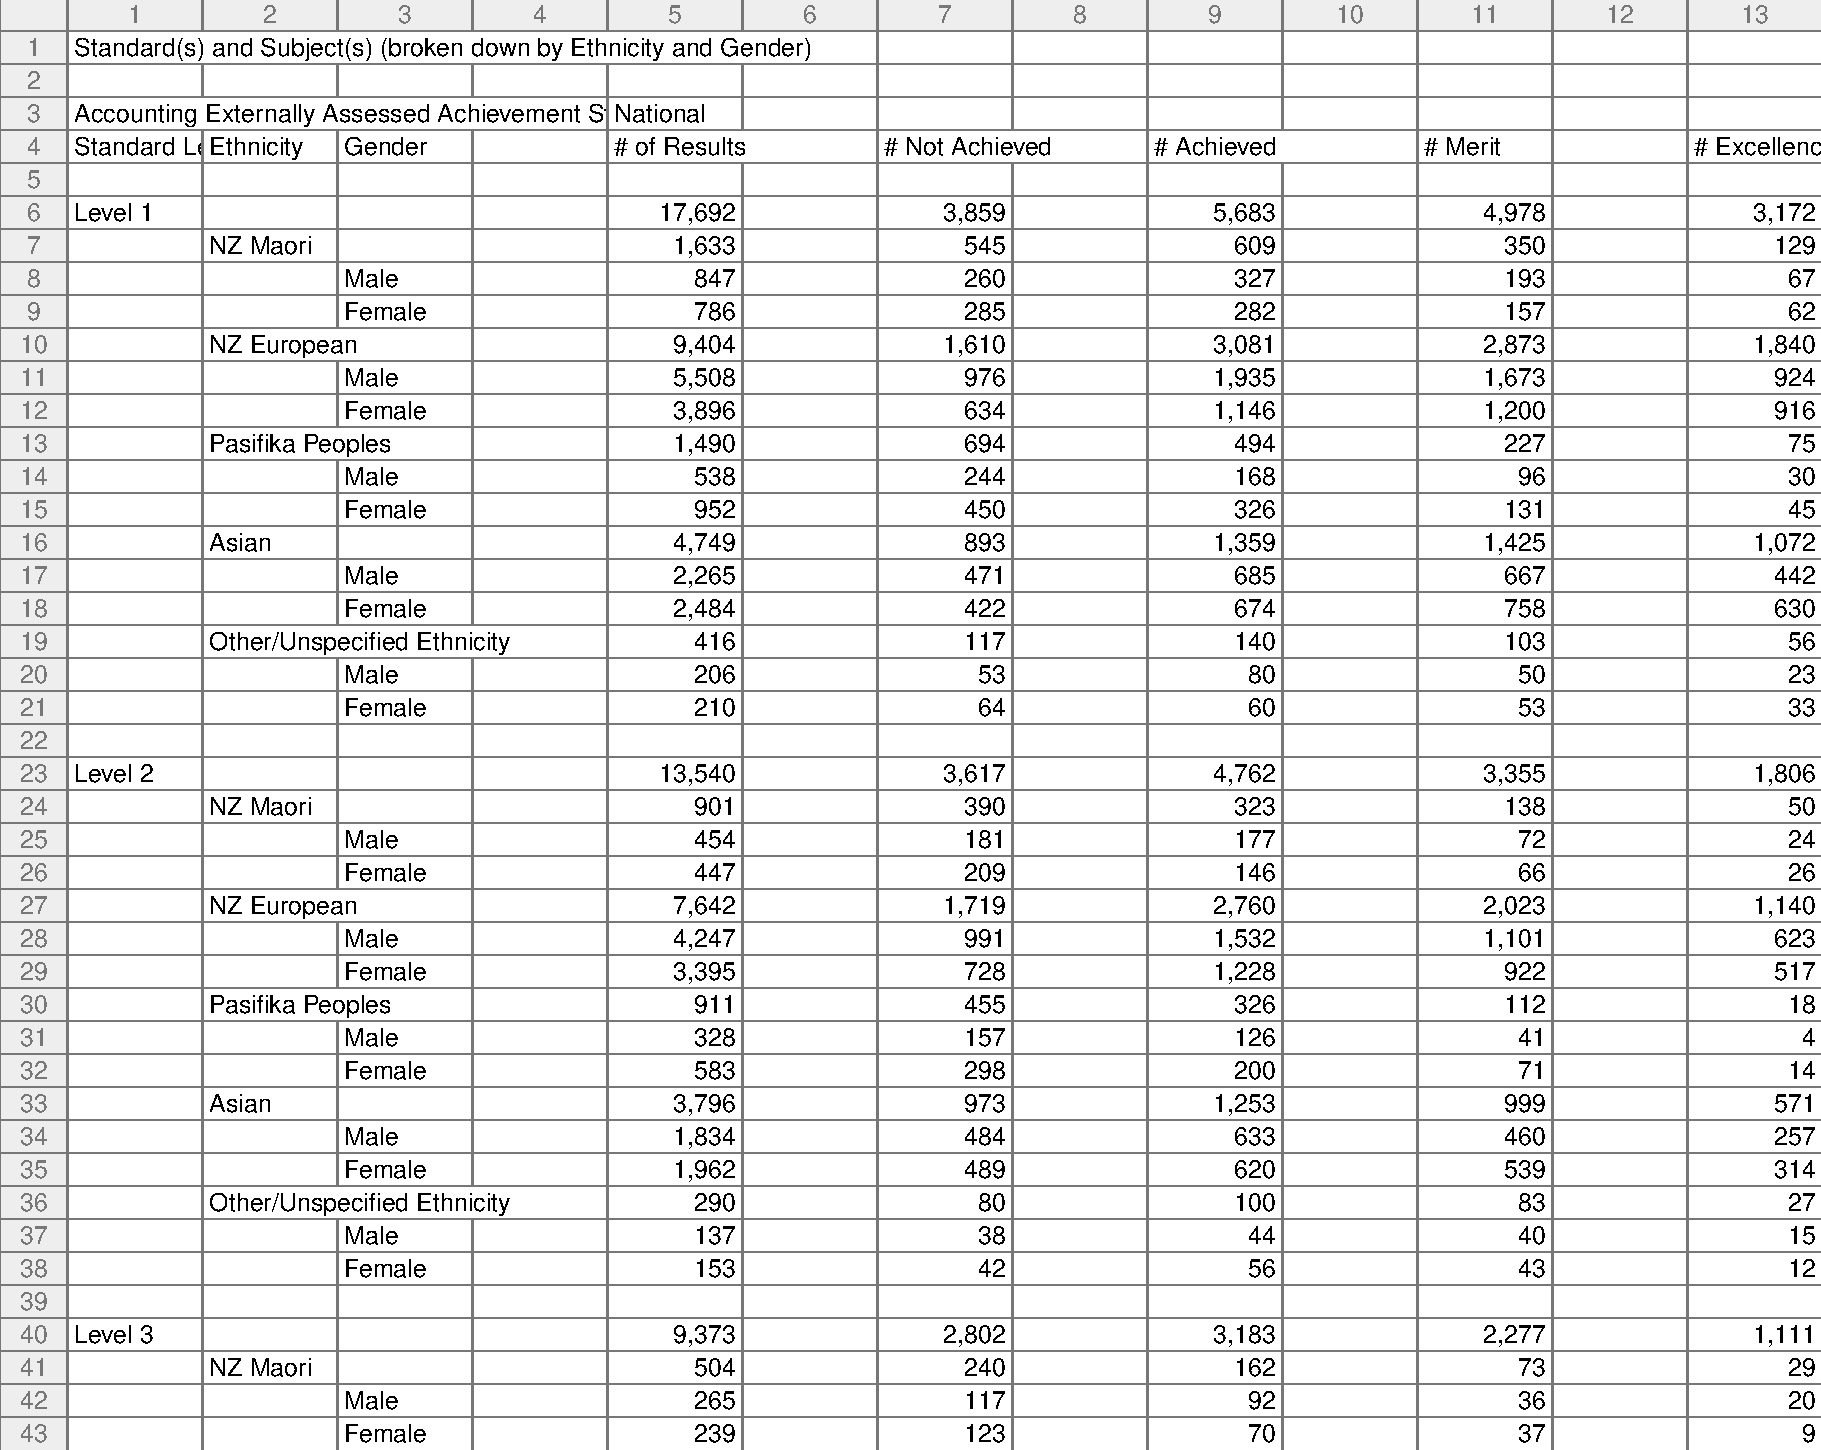
\includegraphics[width=\textwidth]{./TestCase/NZQASubjects.pdf}
\end{figure}
\begin{verbatim}
> rowData 
[1]  6 55
> colData 
[1]  5 13
> rowslist 
$label
[1] 1 3 4

$data
 [1]  6  7  8  9 10 11 12 13 14 15 16 17 18 19 20 21 23 24 25 26 27 28 29 30 31
[26] 32 33 34 35 36 37 38 40 41 42 43 44 45 46 47 48 49 50 51 52 53 54 55

> colslist 
$label
[1] 1 2 3

$data
[1]  5  7  9 11 13

> res 
$`Level 1`
$`Level 1`$rows
 [1]  2  3  4  5  6  7  8  9 10 11 12 13 14 15 16

$`Level 1`$cols
[1] 1 2 3


$`Level 2`
$`Level 2`$rows
 [1] 18 19 20 21 22 23 24 25 26 27 28 29 30 31 32

$`Level 2`$cols
[1] 1 2 3


$`Level 3`
$`Level 3`$rows
 [1] 34 35 36 37 38 39 40 41 42 43 44 45 46 47 48

$`Level 3`$cols
[1] 1 2 3


> res 
$`NZ Maori`
$`NZ Maori`$rows
[1] 3 4

$`NZ Maori`$cols
[1] 2 3


$`NZ European`
$`NZ European`$rows
[1] 6 7

$`NZ European`$cols
[1] 2 3


$`Pasifika Peoples`
$`Pasifika Peoples`$rows
[1]  9 10

$`Pasifika Peoples`$cols
[1] 2 3


$Asian
$Asian$rows
[1] 12 13

$Asian$cols
[1] 2 3


$`Other/Unspecified Ethnicity`
$`Other/Unspecified Ethnicity`$rows
[1] 15 16

$`Other/Unspecified Ethnicity`$cols
[1] 2 3


> plist 
$rows
[1] 3 4

$cols
[1] 3

> res 
  Male Female 
     3      4 
> plist 
$rows
[1] 6 7

$cols
[1] 3

> res 
  Male Female 
     6      7 
> plist 
$rows
[1]  9 10

$cols
[1] 3

> res 
  Male Female 
     9     10 
> plist 
$rows
[1] 12 13

$cols
[1] 3

> res 
  Male Female 
    12     13 
> plist 
$rows
[1] 15 16

$cols
[1] 3

> res 
  Male Female 
    15     16 
> res 
$`NZ Maori`
$`NZ Maori`$rows
[1] 19 20

$`NZ Maori`$cols
[1] 2 3


$`NZ European`
$`NZ European`$rows
[1] 22 23

$`NZ European`$cols
[1] 2 3


$`Pasifika Peoples`
$`Pasifika Peoples`$rows
[1] 25 26

$`Pasifika Peoples`$cols
[1] 2 3


$Asian
$Asian$rows
[1] 28 29

$Asian$cols
[1] 2 3


$`Other/Unspecified Ethnicity`
$`Other/Unspecified Ethnicity`$rows
[1] 31 32

$`Other/Unspecified Ethnicity`$cols
[1] 2 3


> plist 
$rows
[1] 19 20

$cols
[1] 3

> res 
  Male Female 
    19     20 
> plist 
$rows
[1] 22 23

$cols
[1] 3

> res 
  Male Female 
    22     23 
> plist 
$rows
[1] 25 26

$cols
[1] 3

> res 
  Male Female 
    25     26 
> plist 
$rows
[1] 28 29

$cols
[1] 3

> res 
  Male Female 
    28     29 
> plist 
$rows
[1] 31 32

$cols
[1] 3

> res 
  Male Female 
    31     32 
> res 
$`NZ Maori`
$`NZ Maori`$rows
[1] 35 36

$`NZ Maori`$cols
[1] 2 3


$`NZ European`
$`NZ European`$rows
[1] 38 39

$`NZ European`$cols
[1] 2 3


$`Pasifika Peoples`
$`Pasifika Peoples`$rows
[1] 41 42

$`Pasifika Peoples`$cols
[1] 2 3


$Asian
$Asian$rows
[1] 44 45

$Asian$cols
[1] 2 3


$`Other/Unspecified Ethnicity`
$`Other/Unspecified Ethnicity`$rows
[1] 47 48

$`Other/Unspecified Ethnicity`$cols
[1] 2 3


> plist 
$rows
[1] 35 36

$cols
[1] 3

> res 
  Male Female 
    35     36 
> plist 
$rows
[1] 38 39

$cols
[1] 3

> res 
  Male Female 
    38     39 
> plist 
$rows
[1] 41 42

$cols
[1] 3

> res 
  Male Female 
    41     42 
> plist 
$rows
[1] 44 45

$cols
[1] 3

> res 
  Male Female 
    44     45 
> plist 
$rows
[1] 47 48

$cols
[1] 3

> res 
  Male Female 
    47     48 
> rowplist 
$`Level 1`
+ NZ Maori (2, 2)
- + Male (3, 3)
- + Female (4, 3)
+ NZ European (5, 2)
- + Male (6, 3)
- + Female (7, 3)
+ Pasifika Peoples (8, 2)
- + Male (9, 3)
- + Female (10, 3)
+ Asian (11, 2)
- + Male (12, 3)
- + Female (13, 3)
+ Other/Unspecified Ethnicity (14, 2)
- + Male (15, 3)
- + Female (16, 3)

$`Level 2`
+ NZ Maori (18, 2)
- + Male (19, 3)
- + Female (20, 3)
+ NZ European (21, 2)
- + Male (22, 3)
- + Female (23, 3)
+ Pasifika Peoples (24, 2)
- + Male (25, 3)
- + Female (26, 3)
+ Asian (27, 2)
- + Male (28, 3)
- + Female (29, 3)
+ Other/Unspecified Ethnicity (30, 2)
- + Male (31, 3)
- + Female (32, 3)

$`Level 3`
+ NZ Maori (34, 2)
- + Male (35, 3)
- + Female (36, 3)
+ NZ European (37, 2)
- + Male (38, 3)
- + Female (39, 3)
+ Pasifika Peoples (40, 2)
- + Male (41, 3)
- + Female (42, 3)
+ Asian (43, 2)
- + Male (44, 3)
- + Female (45, 3)
+ Other/Unspecified Ethnicity (46, 2)
- + Male (47, 3)
- + Female (48, 3)

> rowvecs 
     [,1]      [,2]               [,3]    
[1,] "Level 1" "NZ Maori"         "Male"  
[2,] "Level 1" "NZ Maori"         "Female"
[3,] "Level 1" "NZ European"      "Male"  
[4,] "Level 1" "NZ European"      "Female"
[5,] "Level 1" "Pasifika Peoples" "Male"  
[6,] "Level 1" "Pasifika Peoples" "Female"
> matColLabel 
     V5             V7               V9           V11       V13           
[1,] NA             NA               NA           NA        NA            
[2,] "National"     NA               NA           NA        NA            
[3,] "# of Results" "# Not Achieved" "# Achieved" "# Merit" "# Excellence"
> cursub 
        V5         V7         V9        V11        V13 
"National"         NA         NA         NA         NA 
> currow[curcols] 
        V5         V7         V9        V11        V13 
"National"         NA         NA         NA         NA 
> cursub 
              V5               V7               V9              V11 
  "# of Results" "# Not Achieved"     "# Achieved"        "# Merit" 
             V13 
  "# Excellence" 
> currow[curcols] 
              V5               V7               V9              V11 
  "# of Results" "# Not Achieved"     "# Achieved"        "# Merit" 
             V13 
  "# Excellence" 
> matColLabel 
     V5             V7               V9           V11       V13           
[1,] NA             NA               NA           NA        NA            
[2,] "National"     NA               NA           NA        NA            
[3,] "# of Results" "# Not Achieved" "# Achieved" "# Merit" "# Excellence"
> matColLabel 
     V5             V7               V9           V11       V13           
[1,] NA             NA               NA           NA        NA            
[2,] "National"     NA               NA           NA        NA            
[3,] "# of Results" "# Not Achieved" "# Achieved" "# Merit" "# Excellence"
> matColLabel 
     V5             V7               V9           V11       V13           
[1,] NA             NA               NA           NA        NA            
[2,] "National"     NA               NA           NA        NA            
[3,] "# of Results" "# Not Achieved" "# Achieved" "# Merit" "# Excellence"
> res 
$National
$National$rows
[1] 1 2 3 4 5

$National$cols
[1] 3


> plist 
$rows
[1] 1 2 3 4 5

$cols
[1] 3

> res 
  # of Results # Not Achieved     # Achieved        # Merit   # Excellence 
             1              2              3              4              5 
> plist 
  # of Results # Not Achieved     # Achieved        # Merit   # Excellence 
             1              2              3              4              5 
> matData 
     V5       V7      V9       V11      V13    
[1,] "847.0"  "260.0" "327.0"  "193.0"  "67.0" 
[2,] "786.0"  "285.0" "282.0"  "157.0"  "62.0" 
[3,] "5508.0" "976.0" "1935.0" "1673.0" "924.0"
[4,] "3896.0" "634.0" "1146.0" "1200.0" "916.0"
[5,] "538.0"  "244.0" "168.0"  "96.0"   "30.0" 
[6,] "952.0"  "450.0" "326.0"  "131.0"  "45.0" 
> datbit 
     V5       V7      V9       V11      V13    
[1,] "847.0"  "260.0" "327.0"  "193.0"  "67.0" 
[2,] "786.0"  "285.0" "282.0"  "157.0"  "62.0" 
[3,] "5508.0" "976.0" "1935.0" "1673.0" "924.0"
[4,] "3896.0" "634.0" "1146.0" "1200.0" "916.0"
[5,] "538.0"  "244.0" "168.0"  "96.0"   "30.0" 
[6,] "952.0"  "450.0" "326.0"  "131.0"  "45.0" 
> colplist 
$National
+ # of Results (1, 3)
+ # Not Achieved (2, 3)
+ # Achieved (3, 3)
+ # Merit (4, 3)
+ # Excellence (5, 3)

> res 
   UNKNOWN UNKNOWN          UNKNOWN UNKNOWN # of Results # Not Achieved
1 National Level 1         NZ Maori    Male          847            260
2 National Level 1         NZ Maori  Female          786            285
3 National Level 1      NZ European    Male         5508            976
4 National Level 1      NZ European  Female         3896            634
5 National Level 1 Pasifika Peoples    Male          538            244
6 National Level 1 Pasifika Peoples  Female          952            450
  # Achieved # Merit # Excellence
1        327     193           67
2        282     157           62
3       1935    1673          924
4       1146    1200          916
5        168      96           30
6        326     131           45
\end{verbatim}

\newpage
\subsection{StatsNZGDP.csv}
\label{sec:TCRO_StatsNZGDP.csv}
\begin{figure}[!h]
\centering
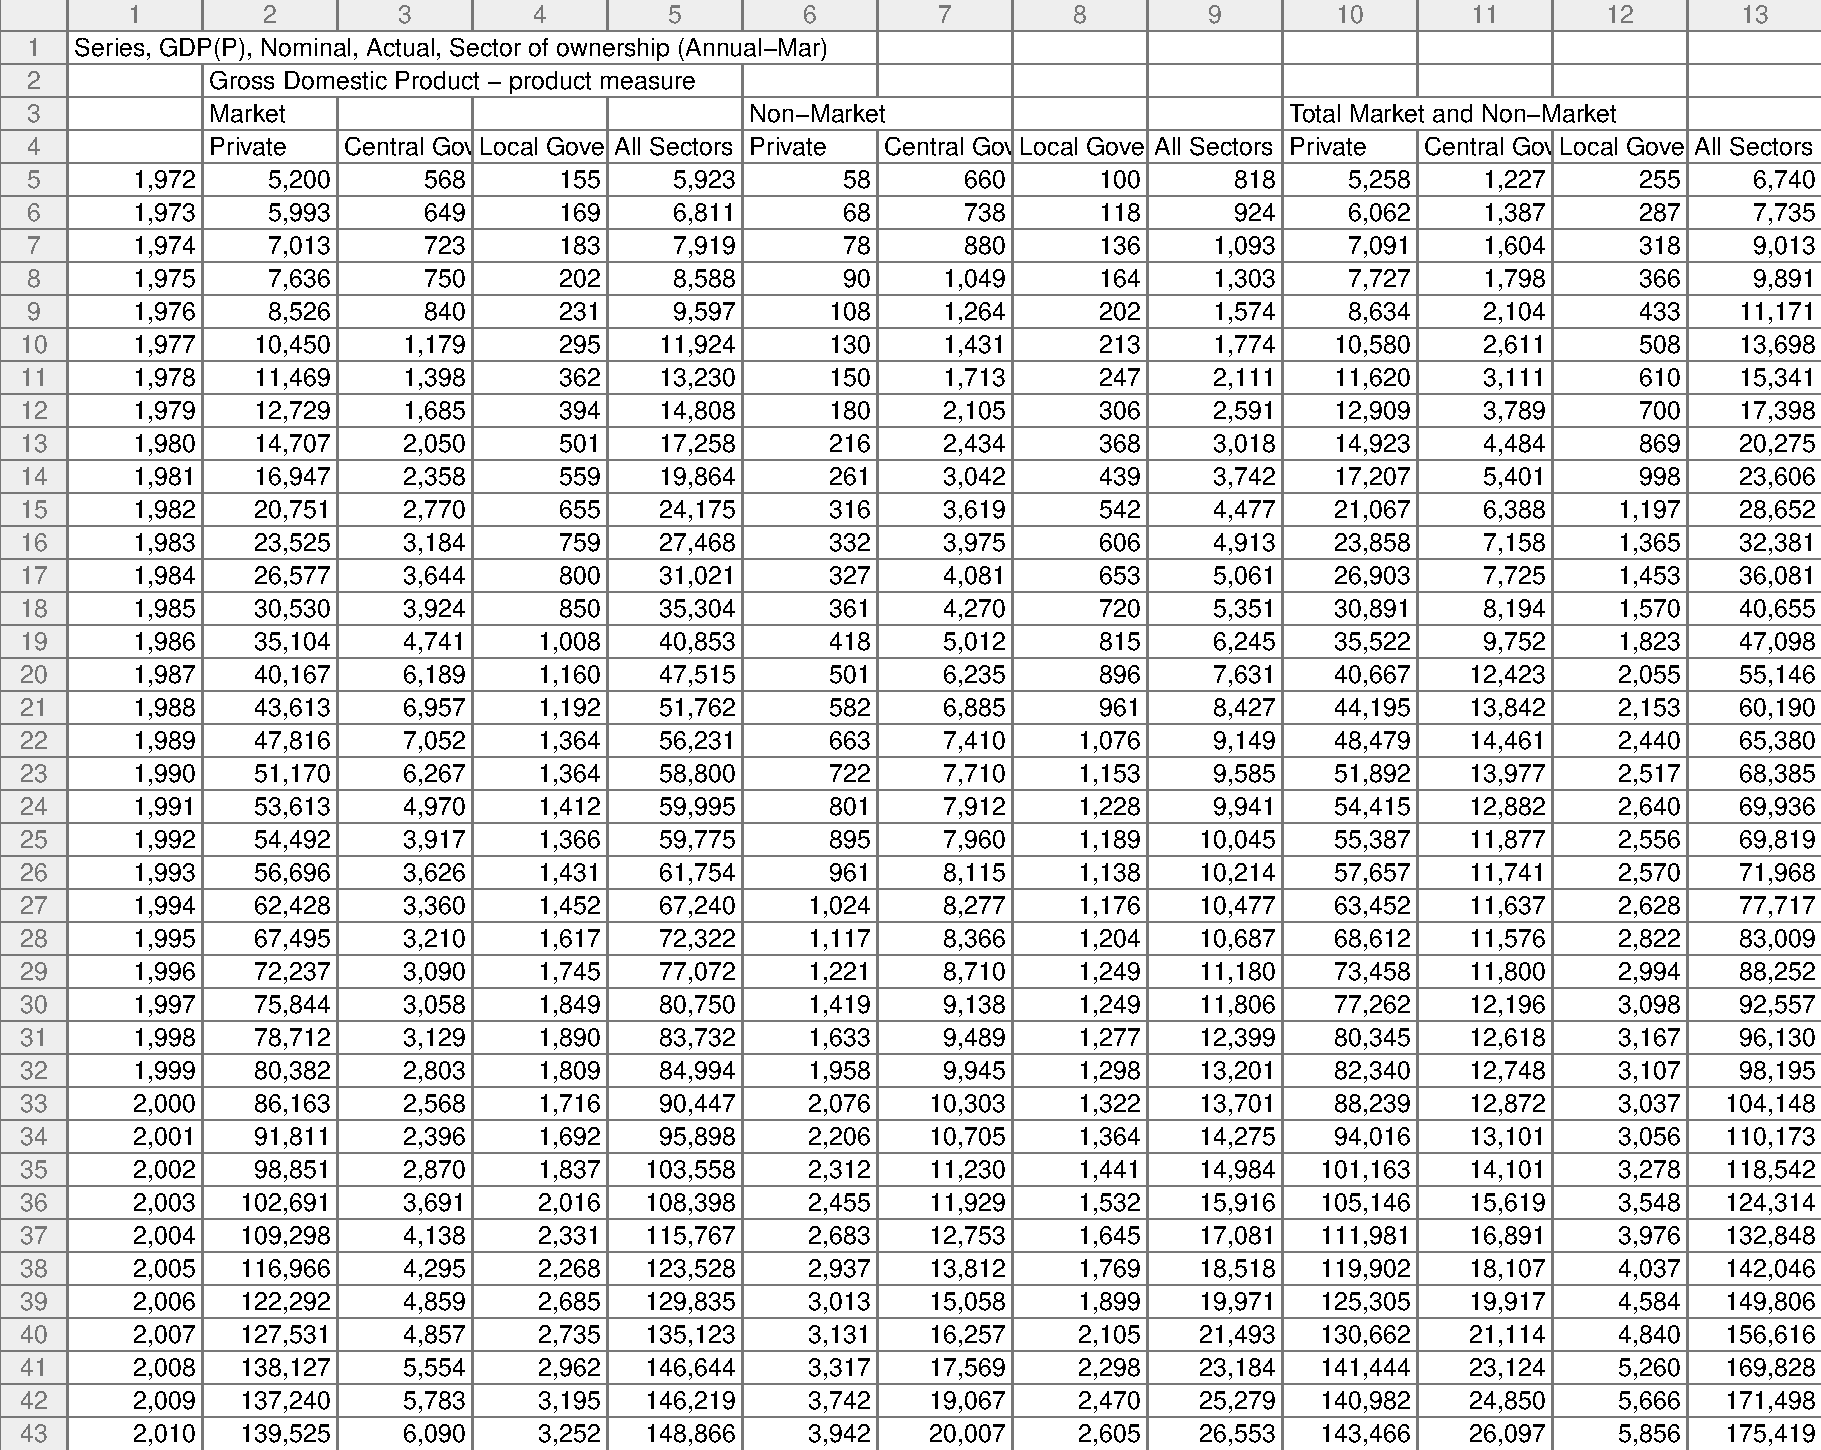
\includegraphics[width=\textwidth]{./TestCase/StatsNZGDP.pdf}
\end{figure}
\begin{verbatim}
> rowData 
[1]  5 43
> colData 
[1]  1 37
> rowslist 
$label
[1] 1 2 3 4

$data
 [1]  5  6  7  8  9 10 11 12 13 14 15 16 17 18 19 20 21 22 23 24 25 26 27 28 29
[26] 30 31 32 33 34 35 36 37 38 39 40 41 42 43

> colslist 
$label
integer(0)

$data
 [1]  1  2  3  4  5  6  7  8  9 10 11 12 13 14 15 16 17 18 19 20 21 22 23 24 25
[26] 26 27 28 29 30 31 32 33 34 35 36 37

> plist 
$rows
 [1]  1  2  3  4  5  6  7  8  9 10 11 12 13 14 15 16 17 18 19 20 21 22 23 24 25
[26] 26 27 28 29 30 31 32 33 34 35 36 37 38 39

$cols
[1] 1

> res 
1972 1973 1974 1975 1976 1977 
   1    2    3    4    5    6 
> rowplist 
1972 1973 1974 1975 1976 1977 
   1    2    3    4    5    6 
> rowvecs 
     [,1]  
[1,] "1972"
[2,] "1973"
[3,] "1974"
[4,] "1975"
[5,] "1976"
[6,] "1977"
> matColLabel 
     V2                                         V3                         
[1,] NA                                         NA                         
[2,] "Gross Domestic Product - product measure" NA                         
[3,] "Market"                                   NA                         
[4,] "Private"                                  "Central Government Sector"
     V4                        V5            V6          
[1,] NA                        NA            NA          
[2,] NA                        NA            NA          
[3,] NA                        NA            "Non-Market"
[4,] "Local Government Sector" "All Sectors" "Private"   
     V7                         
[1,] NA                         
[2,] NA                         
[3,] NA                         
[4,] "Central Government Sector"
> cursub 
                                        V2 
"Gross Domestic Product - product measure" 
                                        V3 
                                        NA 
                                        V4 
                                        NA 
                                        V5 
                                        NA 
                                        V6 
                                        NA 
                                        V7 
                                        NA 
> currow[curcols] 
                                        V2 
"Gross Domestic Product - product measure" 
                                        V3 
                                        NA 
                                        V4 
                                        NA 
                                        V5 
                                        NA 
                                        V6 
                                        NA 
                                        V7 
                                        NA 
> cursub 
     V14      V15      V16      V17      V18      V19 
"Output"       NA       NA       NA       NA       NA 
> currow[curcols] 
     V14      V15      V16      V17      V18      V19 
"Output"       NA       NA       NA       NA       NA 
> cursub 
                       V26                        V27 
"Intermediate Consumption"                         NA 
                       V28                        V29 
                        NA                         NA 
                       V30                        V31 
                        NA                         NA 
> currow[curcols] 
                       V26                        V27 
"Intermediate Consumption"                         NA 
                       V28                        V29 
                        NA                         NA 
                       V30                        V31 
                        NA                         NA 
> cursub 
      V2       V3       V4       V5 
"Market"       NA       NA       NA 
> currow[curcols] 
      V2       V3       V4       V5 
"Market"       NA       NA       NA 
> cursub 
          V6           V7           V8           V9 
"Non-Market"           NA           NA           NA 
> currow[curcols] 
          V6           V7           V8           V9 
"Non-Market"           NA           NA           NA 
> cursub 
                          V10                           V11 
"Total Market and Non-Market"                            NA 
                          V12                           V13 
                           NA                            NA 
> currow[curcols] 
                          V10                           V11 
"Total Market and Non-Market"                            NA 
                          V12                           V13 
                           NA                            NA 
> cursub 
     V14      V15      V16      V17 
"Market"       NA       NA       NA 
> currow[curcols] 
     V14      V15      V16      V17 
"Market"       NA       NA       NA 
> cursub 
         V18          V19          V20          V21 
"Non-Market"           NA           NA           NA 
> currow[curcols] 
         V18          V19          V20          V21 
"Non-Market"           NA           NA           NA 
> cursub 
                          V22                           V23 
"Total Market and Non-Market"                            NA 
                          V24                           V25 
                           NA                            NA 
> currow[curcols] 
                          V22                           V23 
"Total Market and Non-Market"                            NA 
                          V24                           V25 
                           NA                            NA 
> cursub 
     V26      V27      V28      V29 
"Market"       NA       NA       NA 
> currow[curcols] 
     V26      V27      V28      V29 
"Market"       NA       NA       NA 
> cursub 
         V30          V31          V32          V33 
"Non-Market"           NA           NA           NA 
> currow[curcols] 
         V30          V31          V32          V33 
"Non-Market"           NA           NA           NA 
> cursub 
                          V34                           V35 
"Total Market and Non-Market"                            NA 
                          V36                           V37 
                           NA                            NA 
> currow[curcols] 
                          V34                           V35 
"Total Market and Non-Market"                            NA 
                          V36                           V37 
                           NA                            NA 
> cursub 
                         V2                          V3 
                  "Private" "Central Government Sector" 
                         V4                          V5 
  "Local Government Sector"               "All Sectors" 
> currow[curcols] 
                         V2                          V3 
                  "Private" "Central Government Sector" 
                         V4                          V5 
  "Local Government Sector"               "All Sectors" 
> cursub 
                         V6                          V7 
                  "Private" "Central Government Sector" 
                         V8                          V9 
  "Local Government Sector"               "All Sectors" 
> currow[curcols] 
                         V6                          V7 
                  "Private" "Central Government Sector" 
                         V8                          V9 
  "Local Government Sector"               "All Sectors" 
> cursub 
                        V10                         V11 
                  "Private" "Central Government Sector" 
                        V12                         V13 
  "Local Government Sector"               "All Sectors" 
> currow[curcols] 
                        V10                         V11 
                  "Private" "Central Government Sector" 
                        V12                         V13 
  "Local Government Sector"               "All Sectors" 
> cursub 
                        V14                         V15 
                  "Private" "Central Government Sector" 
                        V16                         V17 
  "Local Government Sector"               "All Sectors" 
> currow[curcols] 
                        V14                         V15 
                  "Private" "Central Government Sector" 
                        V16                         V17 
  "Local Government Sector"               "All Sectors" 
> cursub 
                        V18                         V19 
                  "Private" "Central Government Sector" 
                        V20                         V21 
  "Local Government Sector"               "All Sectors" 
> currow[curcols] 
                        V18                         V19 
                  "Private" "Central Government Sector" 
                        V20                         V21 
  "Local Government Sector"               "All Sectors" 
> cursub 
                        V22                         V23 
                  "Private" "Central Government Sector" 
                        V24                         V25 
  "Local Government Sector"               "All Sectors" 
> currow[curcols] 
                        V22                         V23 
                  "Private" "Central Government Sector" 
                        V24                         V25 
  "Local Government Sector"               "All Sectors" 
> cursub 
                        V26                         V27 
                  "Private" "Central Government Sector" 
                        V28                         V29 
  "Local Government Sector"               "All Sectors" 
> currow[curcols] 
                        V26                         V27 
                  "Private" "Central Government Sector" 
                        V28                         V29 
  "Local Government Sector"               "All Sectors" 
> cursub 
                        V30                         V31 
                  "Private" "Central Government Sector" 
                        V32                         V33 
  "Local Government Sector"               "All Sectors" 
> currow[curcols] 
                        V30                         V31 
                  "Private" "Central Government Sector" 
                        V32                         V33 
  "Local Government Sector"               "All Sectors" 
> cursub 
                        V34                         V35 
                  "Private" "Central Government Sector" 
                        V36                         V37 
  "Local Government Sector"               "All Sectors" 
> currow[curcols] 
                        V34                         V35 
                  "Private" "Central Government Sector" 
                        V36                         V37 
  "Local Government Sector"               "All Sectors" 
> matColLabel 
     V2                                         V3                         
[1,] NA                                         NA                         
[2,] "Gross Domestic Product - product measure" NA                         
[3,] "Market"                                   NA                         
[4,] "Private"                                  "Central Government Sector"
     V4                        V5            V6          
[1,] NA                        NA            NA          
[2,] NA                        NA            NA          
[3,] NA                        NA            "Non-Market"
[4,] "Local Government Sector" "All Sectors" "Private"   
     V7                         
[1,] NA                         
[2,] NA                         
[3,] NA                         
[4,] "Central Government Sector"
> matColLabel 
     V2                                         V3                         
[1,] NA                                         NA                         
[2,] "Gross Domestic Product - product measure" NA                         
[3,] "Market"                                   NA                         
[4,] "Private"                                  "Central Government Sector"
     V4                        V5            V6          
[1,] NA                        NA            NA          
[2,] NA                        NA            NA          
[3,] NA                        NA            "Non-Market"
[4,] "Local Government Sector" "All Sectors" "Private"   
     V7                         
[1,] NA                         
[2,] NA                         
[3,] NA                         
[4,] "Central Government Sector"
> matColLabel 
     V2                                         V3                         
[1,] NA                                         NA                         
[2,] "Gross Domestic Product - product measure" NA                         
[3,] "Market"                                   NA                         
[4,] "Private"                                  "Central Government Sector"
     V4                        V5            V6          
[1,] NA                        NA            NA          
[2,] NA                        NA            NA          
[3,] NA                        NA            "Non-Market"
[4,] "Local Government Sector" "All Sectors" "Private"   
     V7                         
[1,] NA                         
[2,] NA                         
[3,] NA                         
[4,] "Central Government Sector"
> res 
$`Gross Domestic Product - product measure`
$`Gross Domestic Product - product measure`$rows
 [1]  1  2  3  4  5  6  7  8  9 10 11 12

$`Gross Domestic Product - product measure`$cols
[1] 3 4


$Output
$Output$rows
 [1] 13 14 15 16 17 18 19 20 21 22 23 24

$Output$cols
[1] 3 4


$`Intermediate Consumption`
$`Intermediate Consumption`$rows
 [1] 25 26 27 28 29 30 31 32 33 34 35 36

$`Intermediate Consumption`$cols
[1] 3 4


> res 
$Market
$Market$rows
[1] 1 2 3 4

$Market$cols
[1] 4


$`Non-Market`
$`Non-Market`$rows
[1] 5 6 7 8

$`Non-Market`$cols
[1] 4


$`Total Market and Non-Market`
$`Total Market and Non-Market`$rows
[1]  9 10 11 12

$`Total Market and Non-Market`$cols
[1] 4


> plist 
$rows
[1] 1 2 3 4

$cols
[1] 4

> res 
                  Private Central Government Sector   Local Government Sector 
                        1                         2                         3 
              All Sectors 
                        4 
> plist 
$rows
[1] 5 6 7 8

$cols
[1] 4

> res 
                  Private Central Government Sector   Local Government Sector 
                        5                         6                         7 
              All Sectors 
                        8 
> plist 
$rows
[1]  9 10 11 12

$cols
[1] 4

> res 
                  Private Central Government Sector   Local Government Sector 
                        9                        10                        11 
              All Sectors 
                       12 
> res 
$Market
$Market$rows
[1] 13 14 15 16

$Market$cols
[1] 4


$`Non-Market`
$`Non-Market`$rows
[1] 17 18 19 20

$`Non-Market`$cols
[1] 4


$`Total Market and Non-Market`
$`Total Market and Non-Market`$rows
[1] 21 22 23 24

$`Total Market and Non-Market`$cols
[1] 4


> plist 
$rows
[1] 13 14 15 16

$cols
[1] 4

> res 
                  Private Central Government Sector   Local Government Sector 
                       13                        14                        15 
              All Sectors 
                       16 
> plist 
$rows
[1] 17 18 19 20

$cols
[1] 4

> res 
                  Private Central Government Sector   Local Government Sector 
                       17                        18                        19 
              All Sectors 
                       20 
> plist 
$rows
[1] 21 22 23 24

$cols
[1] 4

> res 
                  Private Central Government Sector   Local Government Sector 
                       21                        22                        23 
              All Sectors 
                       24 
> res 
$Market
$Market$rows
[1] 25 26 27 28

$Market$cols
[1] 4


$`Non-Market`
$`Non-Market`$rows
[1] 29 30 31 32

$`Non-Market`$cols
[1] 4


$`Total Market and Non-Market`
$`Total Market and Non-Market`$rows
[1] 33 34 35 36

$`Total Market and Non-Market`$cols
[1] 4


> plist 
$rows
[1] 25 26 27 28

$cols
[1] 4

> res 
                  Private Central Government Sector   Local Government Sector 
                       25                        26                        27 
              All Sectors 
                       28 
> plist 
$rows
[1] 29 30 31 32

$cols
[1] 4

> res 
                  Private Central Government Sector   Local Government Sector 
                       29                        30                        31 
              All Sectors 
                       32 
> plist 
$rows
[1] 33 34 35 36

$cols
[1] 4

> res 
                  Private Central Government Sector   Local Government Sector 
                       33                        34                        35 
              All Sectors 
                       36 
> plist 
                  Private Central Government Sector   Local Government Sector 
                        1                         2                         3 
              All Sectors 
                        4 
> matData 
     V2      V3     V4    V5      V6    V7    
[1,] "5200"  "568"  "155" "5923"  "58"  "660" 
[2,] "5993"  "649"  "169" "6811"  "68"  "738" 
[3,] "7013"  "723"  "183" "7919"  "78"  "880" 
[4,] "7636"  "750"  "202" "8588"  "90"  "1049"
[5,] "8526"  "840"  "231" "9597"  "108" "1264"
[6,] "10450" "1179" "295" "11924" "130" "1431"
> datbit 
     V2      V3     V4    V5     
[1,] "5200"  "568"  "155" "5923" 
[2,] "5993"  "649"  "169" "6811" 
[3,] "7013"  "723"  "183" "7919" 
[4,] "7636"  "750"  "202" "8588" 
[5,] "8526"  "840"  "231" "9597" 
[6,] "10450" "1179" "295" "11924"
> plist 
                  Private Central Government Sector   Local Government Sector 
                        5                         6                         7 
              All Sectors 
                        8 
> matData 
     V2      V3     V4    V5      V6    V7    
[1,] "5200"  "568"  "155" "5923"  "58"  "660" 
[2,] "5993"  "649"  "169" "6811"  "68"  "738" 
[3,] "7013"  "723"  "183" "7919"  "78"  "880" 
[4,] "7636"  "750"  "202" "8588"  "90"  "1049"
[5,] "8526"  "840"  "231" "9597"  "108" "1264"
[6,] "10450" "1179" "295" "11924" "130" "1431"
> datbit 
     V6    V7     V8    V9    
[1,] "58"  "660"  "100" "818" 
[2,] "68"  "738"  "118" "924" 
[3,] "78"  "880"  "136" "1093"
[4,] "90"  "1049" "164" "1303"
[5,] "108" "1264" "202" "1574"
[6,] "130" "1431" "213" "1774"
> plist 
                  Private Central Government Sector   Local Government Sector 
                        9                        10                        11 
              All Sectors 
                       12 
> matData 
     V2      V3     V4    V5      V6    V7    
[1,] "5200"  "568"  "155" "5923"  "58"  "660" 
[2,] "5993"  "649"  "169" "6811"  "68"  "738" 
[3,] "7013"  "723"  "183" "7919"  "78"  "880" 
[4,] "7636"  "750"  "202" "8588"  "90"  "1049"
[5,] "8526"  "840"  "231" "9597"  "108" "1264"
[6,] "10450" "1179" "295" "11924" "130" "1431"
> datbit 
     V10     V11    V12   V13    
[1,] "5258"  "1227" "255" "6740" 
[2,] "6062"  "1387" "287" "7735" 
[3,] "7091"  "1604" "318" "9013" 
[4,] "7727"  "1798" "366" "9891" 
[5,] "8634"  "2104" "433" "11171"
[6,] "10580" "2611" "508" "13698"
> plist 
                  Private Central Government Sector   Local Government Sector 
                       13                        14                        15 
              All Sectors 
                       16 
> matData 
     V2      V3     V4    V5      V6    V7    
[1,] "5200"  "568"  "155" "5923"  "58"  "660" 
[2,] "5993"  "649"  "169" "6811"  "68"  "738" 
[3,] "7013"  "723"  "183" "7919"  "78"  "880" 
[4,] "7636"  "750"  "202" "8588"  "90"  "1049"
[5,] "8526"  "840"  "231" "9597"  "108" "1264"
[6,] "10450" "1179" "295" "11924" "130" "1431"
> datbit 
     V14     V15    V16   V17    
[1,] "10994" "1005" "357" "12355"
[2,] "13021" "1111" "391" "14523"
[3,] "15370" "1232" "429" "17031"
[4,] "17264" "1453" "492" "19210"
[5,] "20239" "1784" "574" "22597"
[6,] "25121" "2239" "733" "28092"
> plist 
                  Private Central Government Sector   Local Government Sector 
                       17                        18                        19 
              All Sectors 
                       20 
> matData 
     V2      V3     V4    V5      V6    V7    
[1,] "5200"  "568"  "155" "5923"  "58"  "660" 
[2,] "5993"  "649"  "169" "6811"  "68"  "738" 
[3,] "7013"  "723"  "183" "7919"  "78"  "880" 
[4,] "7636"  "750"  "202" "8588"  "90"  "1049"
[5,] "8526"  "840"  "231" "9597"  "108" "1264"
[6,] "10450" "1179" "295" "11924" "130" "1431"
> datbit 
     V18   V19    V20   V21   
[1,] "113" "884"  "179" "1176"
[2,] "129" "987"  "223" "1339"
[3,] "145" "1147" "262" "1554"
[4,] "170" "1384" "328" "1882"
[5,] "196" "1673" "392" "2261"
[6,] "245" "1918" "415" "2578"
> plist 
                  Private Central Government Sector   Local Government Sector 
                       21                        22                        23 
              All Sectors 
                       24 
> matData 
     V2      V3     V4    V5      V6    V7    
[1,] "5200"  "568"  "155" "5923"  "58"  "660" 
[2,] "5993"  "649"  "169" "6811"  "68"  "738" 
[3,] "7013"  "723"  "183" "7919"  "78"  "880" 
[4,] "7636"  "750"  "202" "8588"  "90"  "1049"
[5,] "8526"  "840"  "231" "9597"  "108" "1264"
[6,] "10450" "1179" "295" "11924" "130" "1431"
> datbit 
     V22     V23    V24    V25    
[1,] "11107" "1889" "535"  "13531"
[2,] "13149" "2098" "614"  "15862"
[3,] "15515" "2379" "691"  "18586"
[4,] "17434" "2837" "820"  "21092"
[5,] "20435" "3457" "966"  "24859"
[6,] "25366" "4157" "1147" "30670"
> plist 
                  Private Central Government Sector   Local Government Sector 
                       25                        26                        27 
              All Sectors 
                       28 
> matData 
     V2      V3     V4    V5      V6    V7    
[1,] "5200"  "568"  "155" "5923"  "58"  "660" 
[2,] "5993"  "649"  "169" "6811"  "68"  "738" 
[3,] "7013"  "723"  "183" "7919"  "78"  "880" 
[4,] "7636"  "750"  "202" "8588"  "90"  "1049"
[5,] "8526"  "840"  "231" "9597"  "108" "1264"
[6,] "10450" "1179" "295" "11924" "130" "1431"
> datbit 
     V26     V27    V28   V29    
[1,] "5793"  "437"  "202" "6432" 
[2,] "7027"  "463"  "222" "7712" 
[3,] "8357"  "508"  "247" "9112" 
[4,] "9628"  "704"  "290" "10622"
[5,] "11713" "944"  "343" "13000"
[6,] "14671" "1060" "437" "16168"
> plist 
                  Private Central Government Sector   Local Government Sector 
                       29                        30                        31 
              All Sectors 
                       32 
> matData 
     V2      V3     V4    V5      V6    V7    
[1,] "5200"  "568"  "155" "5923"  "58"  "660" 
[2,] "5993"  "649"  "169" "6811"  "68"  "738" 
[3,] "7013"  "723"  "183" "7919"  "78"  "880" 
[4,] "7636"  "750"  "202" "8588"  "90"  "1049"
[5,] "8526"  "840"  "231" "9597"  "108" "1264"
[6,] "10450" "1179" "295" "11924" "130" "1431"
> datbit 
     V30   V31   V32   V33  
[1,] "56"  "224" "78"  "359"
[2,] "60"  "249" "106" "415"
[3,] "67"  "267" "127" "461"
[4,] "80"  "335" "164" "579"
[5,] "88"  "409" "190" "687"
[6,] "116" "487" "202" "804"
> plist 
                  Private Central Government Sector   Local Government Sector 
                       33                        34                        35 
              All Sectors 
                       36 
> matData 
     V2      V3     V4    V5      V6    V7    
[1,] "5200"  "568"  "155" "5923"  "58"  "660" 
[2,] "5993"  "649"  "169" "6811"  "68"  "738" 
[3,] "7013"  "723"  "183" "7919"  "78"  "880" 
[4,] "7636"  "750"  "202" "8588"  "90"  "1049"
[5,] "8526"  "840"  "231" "9597"  "108" "1264"
[6,] "10450" "1179" "295" "11924" "130" "1431"
> datbit 
     V34     V35    V36   V37    
[1,] "5849"  "662"  "280" "6791" 
[2,] "7088"  "712"  "327" "8126" 
[3,] "8424"  "775"  "373" "9573" 
[4,] "9708"  "1039" "454" "11201"
[5,] "11801" "1353" "533" "13687"
[6,] "14786" "1547" "639" "16972"
> colplist 
$`Gross Domestic Product - product measure`
+ Market (1, 3)
- + Private (1, 4)
- + Central Government Sector (2, 4)
- + Local Government Sector (3, 4)
- + All Sectors (4, 4)
+ Non-Market (5, 3)
- + Private (5, 4)
- + Central Government Sector (6, 4)
- + Local Government Sector (7, 4)
- + All Sectors (8, 4)
+ Total Market and Non-Market (9, 3)
- + Private (9, 4)
- + Central Government Sector (10, 4)
- + Local Government Sector (11, 4)
- + All Sectors (12, 4)

$Output
+ Market (13, 3)
- + Private (13, 4)
- + Central Government Sector (14, 4)
- + Local Government Sector (15, 4)
- + All Sectors (16, 4)
+ Non-Market (17, 3)
- + Private (17, 4)
- + Central Government Sector (18, 4)
- + Local Government Sector (19, 4)
- + All Sectors (20, 4)
+ Total Market and Non-Market (21, 3)
- + Private (21, 4)
- + Central Government Sector (22, 4)
- + Local Government Sector (23, 4)
- + All Sectors (24, 4)

$`Intermediate Consumption`
+ Market (25, 3)
- + Private (25, 4)
- + Central Government Sector (26, 4)
- + Local Government Sector (27, 4)
- + All Sectors (28, 4)
+ Non-Market (29, 3)
- + Private (29, 4)
- + Central Government Sector (30, 4)
- + Local Government Sector (31, 4)
- + All Sectors (32, 4)
+ Total Market and Non-Market (33, 3)
- + Private (33, 4)
- + Central Government Sector (34, 4)
- + Local Government Sector (35, 4)
- + All Sectors (36, 4)

> res 
                                   UNKNOWN UNKNOWN UNKNOWN Private
1 Gross Domestic Product - product measure  Market    1972    5200
2 Gross Domestic Product - product measure  Market    1973    5993
3 Gross Domestic Product - product measure  Market    1974    7013
4 Gross Domestic Product - product measure  Market    1975    7636
5 Gross Domestic Product - product measure  Market    1976    8526
6 Gross Domestic Product - product measure  Market    1977   10450
  Central Government Sector Local Government Sector All Sectors
1                       568                     155        5923
2                       649                     169        6811
3                       723                     183        7919
4                       750                     202        8588
5                       840                     231        9597
6                      1179                     295       11924
\end{verbatim}

\newpage
\subsection{StatsNZLabourForce.csv}
\label{sec:TCRO_StatsNZLabourForce.csv}
\begin{figure}[!h]
\centering
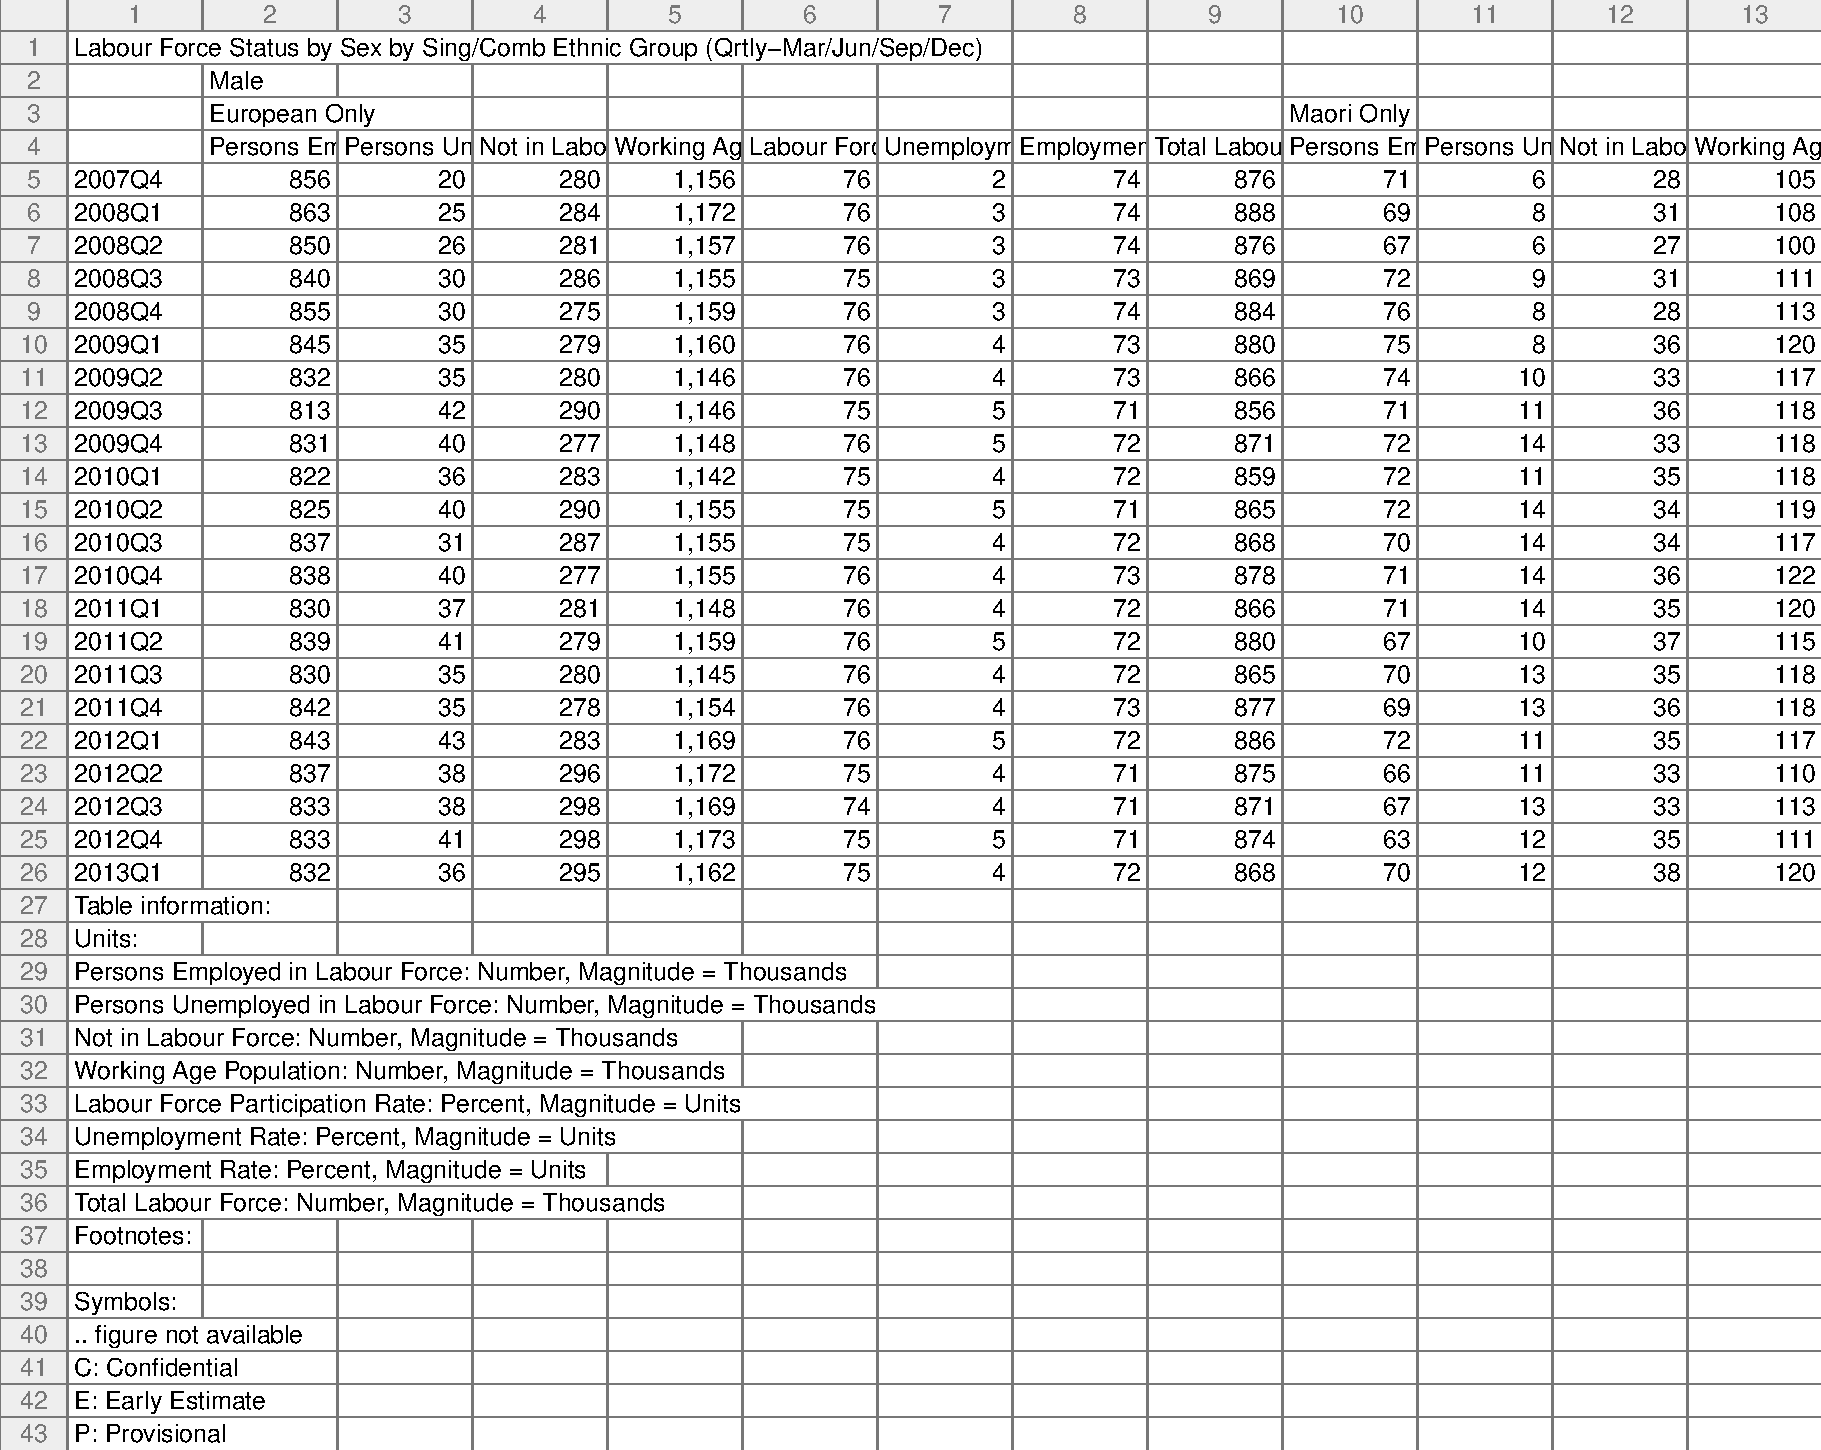
\includegraphics[width=\textwidth]{./TestCase/StatsNZLabourForce.pdf}
\end{figure}
\begin{verbatim}
> rowData 
[1]  5 26
> colData 
[1]   2 241
> rowslist 
$label
[1] 1 2 3 4

$data
 [1]  5  6  7  8  9 10 11 12 13 14 15 16 17 18 19 20 21 22 23 24 25 26

> colslist 
$label
[1] 1

$data
  [1]   2   3   4   5   6   7   8   9  10  11  12  13  14  15  16  17  18  19
 [19]  20  21  22  23  24  25  26  27  28  29  30  31  32  33  34  35  36  37
 [37]  38  39  40  41  42  43  44  45  46  47  48  49  50  51  52  53  54  55
 [55]  56  57  58  59  60  61  62  63  64  65  66  67  68  69  70  71  72  73
 [73]  74  75  76  77  78  79  80  81  82  83  84  85  86  87  88  89  90  91
 [91]  92  93  94  95  96  97  98  99 100 101 102 103 104 105 106 107 108 109
[109] 110 111 112 113 114 115 116 117 118 119 120 121 122 123 124 125 126 127
[127] 128 129 130 131 132 133 134 135 136 137 138 139 140 141 142 143 144 145
[145] 146 147 148 149 150 151 152 153 154 155 156 157 158 159 160 161 162 163
[163] 164 165 166 167 168 169 170 171 172 173 174 175 176 177 178 179 180 181
[181] 182 183 184 185 186 187 188 189 190 191 192 193 194 195 196 197 198 199
[199] 200 201 202 203 204 205 206 207 208 209 210 211 212 213 214 215 216 217
[217] 218 219 220 221 222 223 224 225 226 227 228 229 230 231 232 233 234 235
[235] 236 237 238 239 240 241

> plist 
$rows
 [1]  1  2  3  4  5  6  7  8  9 10 11 12 13 14 15 16 17 18 19 20 21 22

$cols
[1] 1

> res 
2007Q4 2008Q1 2008Q2 2008Q3 2008Q4 2009Q1 
     1      2      3      4      5      6 
> rowplist 
2007Q4 2008Q1 2008Q2 2008Q3 2008Q4 2009Q1 
     1      2      3      4      5      6 
> rowvecs 
     [,1]    
[1,] "2007Q4"
[2,] "2008Q1"
[3,] "2008Q2"
[4,] "2008Q3"
[5,] "2008Q4"
[6,] "2009Q1"
> matColLabel 
     V2                                 V3                                  
[1,] NA                                 NA                                  
[2,] "Male"                             NA                                  
[3,] "European Only"                    NA                                  
[4,] "Persons Employed in Labour Force" "Persons Unemployed in Labour Force"
     V4                    V5                      
[1,] NA                    NA                      
[2,] NA                    NA                      
[3,] NA                    NA                      
[4,] "Not in Labour Force" "Working Age Population"
     V6                                V7                 
[1,] NA                                NA                 
[2,] NA                                NA                 
[3,] NA                                NA                 
[4,] "Labour Force Participation Rate" "Unemployment Rate"
> cursub 
    V2     V3     V4     V5     V6     V7 
"Male"     NA     NA     NA     NA     NA 
> currow[curcols] 
    V2     V3     V4     V5     V6     V7 
"Male"     NA     NA     NA     NA     NA 
> cursub 
     V82      V83      V84      V85      V86      V87 
"Female"       NA       NA       NA       NA       NA 
> currow[curcols] 
     V82      V83      V84      V85      V86      V87 
"Female"       NA       NA       NA       NA       NA 
> cursub 
              V162               V163               V164               V165 
"Total Both Sexes"                 NA                 NA                 NA 
              V166               V167 
                NA                 NA 
> currow[curcols] 
              V162               V163               V164               V165 
"Total Both Sexes"                 NA                 NA                 NA 
              V166               V167 
                NA                 NA 
> cursub 
             V2              V3              V4              V5              V6 
"European Only"              NA              NA              NA              NA 
             V7 
             NA 
> currow[curcols] 
             V2              V3              V4              V5              V6 
"European Only"              NA              NA              NA              NA 
             V7 
             NA 
> cursub 
         V10          V11          V12          V13          V14          V15 
"Maori Only"           NA           NA           NA           NA           NA 
> currow[curcols] 
         V10          V11          V12          V13          V14          V15 
"Maori Only"           NA           NA           NA           NA           NA 
> cursub 
                   V18                    V19                    V20 
"Pacific Peoples Only"                     NA                     NA 
                   V21                    V22                    V23 
                    NA                     NA                     NA 
> currow[curcols] 
                   V18                    V19                    V20 
"Pacific Peoples Only"                     NA                     NA 
                   V21                    V22                    V23 
                    NA                     NA                     NA 
> cursub 
         V26          V27          V28          V29          V30          V31 
"Asian Only"           NA           NA           NA           NA           NA 
> currow[curcols] 
         V26          V27          V28          V29          V30          V31 
"Asian Only"           NA           NA           NA           NA           NA 
> cursub 
         V34          V35          V36          V37          V38          V39 
"MELAA Only"           NA           NA           NA           NA           NA 
> currow[curcols] 
         V34          V35          V36          V37          V38          V39 
"MELAA Only"           NA           NA           NA           NA           NA 
> cursub 
                   V42                    V43                    V44 
"Other Ethnicity Only"                     NA                     NA 
                   V45                    V46                    V47 
                    NA                     NA                     NA 
> currow[curcols] 
                   V42                    V43                    V44 
"Other Ethnicity Only"                     NA                     NA 
                   V45                    V46                    V47 
                    NA                     NA                     NA 
> cursub 
             V50              V51              V52              V53 
"European/Maori"               NA               NA               NA 
             V54              V55 
              NA               NA 
> currow[curcols] 
             V50              V51              V52              V53 
"European/Maori"               NA               NA               NA 
             V54              V55 
              NA               NA 
> cursub 
                                        V58 
"Two or More Groups Not Elsewhere Included" 
                                        V59 
                                         NA 
                                        V60 
                                         NA 
                                        V61 
                                         NA 
                                        V62 
                                         NA 
                                        V63 
                                         NA 
> currow[curcols] 
                                        V58 
"Two or More Groups Not Elsewhere Included" 
                                        V59 
                                         NA 
                                        V60 
                                         NA 
                                        V61 
                                         NA 
                                        V62 
                                         NA 
                                        V63 
                                         NA 
> cursub 
                  V66                   V67                   V68 
"Residual Categories"                    NA                    NA 
                  V69                   V70                   V71 
                   NA                    NA                    NA 
> currow[curcols] 
                  V66                   V67                   V68 
"Residual Categories"                    NA                    NA 
                  V69                   V70                   V71 
                   NA                    NA                    NA 
> cursub 
                      V74                       V75                       V76 
"Total All Ethnic Groups"                        NA                        NA 
                      V77                       V78                       V79 
                       NA                        NA                        NA 
> currow[curcols] 
                      V74                       V75                       V76 
"Total All Ethnic Groups"                        NA                        NA 
                      V77                       V78                       V79 
                       NA                        NA                        NA 
> cursub 
            V82             V83             V84             V85             V86 
"European Only"              NA              NA              NA              NA 
            V87 
             NA 
> currow[curcols] 
            V82             V83             V84             V85             V86 
"European Only"              NA              NA              NA              NA 
            V87 
             NA 
> cursub 
         V90          V91          V92          V93          V94          V95 
"Maori Only"           NA           NA           NA           NA           NA 
> currow[curcols] 
         V90          V91          V92          V93          V94          V95 
"Maori Only"           NA           NA           NA           NA           NA 
> cursub 
                   V98                    V99                   V100 
"Pacific Peoples Only"                     NA                     NA 
                  V101                   V102                   V103 
                    NA                     NA                     NA 
> currow[curcols] 
                   V98                    V99                   V100 
"Pacific Peoples Only"                     NA                     NA 
                  V101                   V102                   V103 
                    NA                     NA                     NA 
> cursub 
        V106         V107         V108         V109         V110         V111 
"Asian Only"           NA           NA           NA           NA           NA 
> currow[curcols] 
        V106         V107         V108         V109         V110         V111 
"Asian Only"           NA           NA           NA           NA           NA 
> cursub 
        V114         V115         V116         V117         V118         V119 
"MELAA Only"           NA           NA           NA           NA           NA 
> currow[curcols] 
        V114         V115         V116         V117         V118         V119 
"MELAA Only"           NA           NA           NA           NA           NA 
> cursub 
                  V122                   V123                   V124 
"Other Ethnicity Only"                     NA                     NA 
                  V125                   V126                   V127 
                    NA                     NA                     NA 
> currow[curcols] 
                  V122                   V123                   V124 
"Other Ethnicity Only"                     NA                     NA 
                  V125                   V126                   V127 
                    NA                     NA                     NA 
> cursub 
            V130             V131             V132             V133 
"European/Maori"               NA               NA               NA 
            V134             V135 
              NA               NA 
> currow[curcols] 
            V130             V131             V132             V133 
"European/Maori"               NA               NA               NA 
            V134             V135 
              NA               NA 
> cursub 
                                       V138 
"Two or More Groups Not Elsewhere Included" 
                                       V139 
                                         NA 
                                       V140 
                                         NA 
                                       V141 
                                         NA 
                                       V142 
                                         NA 
                                       V143 
                                         NA 
> currow[curcols] 
                                       V138 
"Two or More Groups Not Elsewhere Included" 
                                       V139 
                                         NA 
                                       V140 
                                         NA 
                                       V141 
                                         NA 
                                       V142 
                                         NA 
                                       V143 
                                         NA 
> cursub 
                 V146                  V147                  V148 
"Residual Categories"                    NA                    NA 
                 V149                  V150                  V151 
                   NA                    NA                    NA 
> currow[curcols] 
                 V146                  V147                  V148 
"Residual Categories"                    NA                    NA 
                 V149                  V150                  V151 
                   NA                    NA                    NA 
> cursub 
                     V154                      V155                      V156 
"Total All Ethnic Groups"                        NA                        NA 
                     V157                      V158                      V159 
                       NA                        NA                        NA 
> currow[curcols] 
                     V154                      V155                      V156 
"Total All Ethnic Groups"                        NA                        NA 
                     V157                      V158                      V159 
                       NA                        NA                        NA 
> cursub 
           V162            V163            V164            V165            V166 
"European Only"              NA              NA              NA              NA 
           V167 
             NA 
> currow[curcols] 
           V162            V163            V164            V165            V166 
"European Only"              NA              NA              NA              NA 
           V167 
             NA 
> cursub 
        V170         V171         V172         V173         V174         V175 
"Maori Only"           NA           NA           NA           NA           NA 
> currow[curcols] 
        V170         V171         V172         V173         V174         V175 
"Maori Only"           NA           NA           NA           NA           NA 
> cursub 
                  V178                   V179                   V180 
"Pacific Peoples Only"                     NA                     NA 
                  V181                   V182                   V183 
                    NA                     NA                     NA 
> currow[curcols] 
                  V178                   V179                   V180 
"Pacific Peoples Only"                     NA                     NA 
                  V181                   V182                   V183 
                    NA                     NA                     NA 
> cursub 
        V186         V187         V188         V189         V190         V191 
"Asian Only"           NA           NA           NA           NA           NA 
> currow[curcols] 
        V186         V187         V188         V189         V190         V191 
"Asian Only"           NA           NA           NA           NA           NA 
> cursub 
        V194         V195         V196         V197         V198         V199 
"MELAA Only"           NA           NA           NA           NA           NA 
> currow[curcols] 
        V194         V195         V196         V197         V198         V199 
"MELAA Only"           NA           NA           NA           NA           NA 
> cursub 
                  V202                   V203                   V204 
"Other Ethnicity Only"                     NA                     NA 
                  V205                   V206                   V207 
                    NA                     NA                     NA 
> currow[curcols] 
                  V202                   V203                   V204 
"Other Ethnicity Only"                     NA                     NA 
                  V205                   V206                   V207 
                    NA                     NA                     NA 
> cursub 
            V210             V211             V212             V213 
"European/Maori"               NA               NA               NA 
            V214             V215 
              NA               NA 
> currow[curcols] 
            V210             V211             V212             V213 
"European/Maori"               NA               NA               NA 
            V214             V215 
              NA               NA 
> cursub 
                                       V218 
"Two or More Groups Not Elsewhere Included" 
                                       V219 
                                         NA 
                                       V220 
                                         NA 
                                       V221 
                                         NA 
                                       V222 
                                         NA 
                                       V223 
                                         NA 
> currow[curcols] 
                                       V218 
"Two or More Groups Not Elsewhere Included" 
                                       V219 
                                         NA 
                                       V220 
                                         NA 
                                       V221 
                                         NA 
                                       V222 
                                         NA 
                                       V223 
                                         NA 
> cursub 
                 V226                  V227                  V228 
"Residual Categories"                    NA                    NA 
                 V229                  V230                  V231 
                   NA                    NA                    NA 
> currow[curcols] 
                 V226                  V227                  V228 
"Residual Categories"                    NA                    NA 
                 V229                  V230                  V231 
                   NA                    NA                    NA 
> cursub 
                     V234                      V235                      V236 
"Total All Ethnic Groups"                        NA                        NA 
                     V237                      V238                      V239 
                       NA                        NA                        NA 
> currow[curcols] 
                     V234                      V235                      V236 
"Total All Ethnic Groups"                        NA                        NA 
                     V237                      V238                      V239 
                       NA                        NA                        NA 
> cursub 
                                  V2                                   V3 
  "Persons Employed in Labour Force" "Persons Unemployed in Labour Force" 
                                  V4                                   V5 
               "Not in Labour Force"             "Working Age Population" 
                                  V6                                   V7 
   "Labour Force Participation Rate"                  "Unemployment Rate" 
> currow[curcols] 
                                  V2                                   V3 
  "Persons Employed in Labour Force" "Persons Unemployed in Labour Force" 
                                  V4                                   V5 
               "Not in Labour Force"             "Working Age Population" 
                                  V6                                   V7 
   "Labour Force Participation Rate"                  "Unemployment Rate" 
> cursub 
                                 V10                                  V11 
  "Persons Employed in Labour Force" "Persons Unemployed in Labour Force" 
                                 V12                                  V13 
               "Not in Labour Force"             "Working Age Population" 
                                 V14                                  V15 
   "Labour Force Participation Rate"                  "Unemployment Rate" 
> currow[curcols] 
                                 V10                                  V11 
  "Persons Employed in Labour Force" "Persons Unemployed in Labour Force" 
                                 V12                                  V13 
               "Not in Labour Force"             "Working Age Population" 
                                 V14                                  V15 
   "Labour Force Participation Rate"                  "Unemployment Rate" 
> cursub 
                                 V18                                  V19 
  "Persons Employed in Labour Force" "Persons Unemployed in Labour Force" 
                                 V20                                  V21 
               "Not in Labour Force"             "Working Age Population" 
                                 V22                                  V23 
   "Labour Force Participation Rate"                  "Unemployment Rate" 
> currow[curcols] 
                                 V18                                  V19 
  "Persons Employed in Labour Force" "Persons Unemployed in Labour Force" 
                                 V20                                  V21 
               "Not in Labour Force"             "Working Age Population" 
                                 V22                                  V23 
   "Labour Force Participation Rate"                  "Unemployment Rate" 
> cursub 
                                 V26                                  V27 
  "Persons Employed in Labour Force" "Persons Unemployed in Labour Force" 
                                 V28                                  V29 
               "Not in Labour Force"             "Working Age Population" 
                                 V30                                  V31 
   "Labour Force Participation Rate"                  "Unemployment Rate" 
> currow[curcols] 
                                 V26                                  V27 
  "Persons Employed in Labour Force" "Persons Unemployed in Labour Force" 
                                 V28                                  V29 
               "Not in Labour Force"             "Working Age Population" 
                                 V30                                  V31 
   "Labour Force Participation Rate"                  "Unemployment Rate" 
> cursub 
                                 V34                                  V35 
  "Persons Employed in Labour Force" "Persons Unemployed in Labour Force" 
                                 V36                                  V37 
               "Not in Labour Force"             "Working Age Population" 
                                 V38                                  V39 
   "Labour Force Participation Rate"                  "Unemployment Rate" 
> currow[curcols] 
                                 V34                                  V35 
  "Persons Employed in Labour Force" "Persons Unemployed in Labour Force" 
                                 V36                                  V37 
               "Not in Labour Force"             "Working Age Population" 
                                 V38                                  V39 
   "Labour Force Participation Rate"                  "Unemployment Rate" 
> cursub 
                                 V42                                  V43 
  "Persons Employed in Labour Force" "Persons Unemployed in Labour Force" 
                                 V44                                  V45 
               "Not in Labour Force"             "Working Age Population" 
                                 V46                                  V47 
   "Labour Force Participation Rate"                  "Unemployment Rate" 
> currow[curcols] 
                                 V42                                  V43 
  "Persons Employed in Labour Force" "Persons Unemployed in Labour Force" 
                                 V44                                  V45 
               "Not in Labour Force"             "Working Age Population" 
                                 V46                                  V47 
   "Labour Force Participation Rate"                  "Unemployment Rate" 
> cursub 
                                 V50                                  V51 
  "Persons Employed in Labour Force" "Persons Unemployed in Labour Force" 
                                 V52                                  V53 
               "Not in Labour Force"             "Working Age Population" 
                                 V54                                  V55 
   "Labour Force Participation Rate"                  "Unemployment Rate" 
> currow[curcols] 
                                 V50                                  V51 
  "Persons Employed in Labour Force" "Persons Unemployed in Labour Force" 
                                 V52                                  V53 
               "Not in Labour Force"             "Working Age Population" 
                                 V54                                  V55 
   "Labour Force Participation Rate"                  "Unemployment Rate" 
> cursub 
                                 V58                                  V59 
  "Persons Employed in Labour Force" "Persons Unemployed in Labour Force" 
                                 V60                                  V61 
               "Not in Labour Force"             "Working Age Population" 
                                 V62                                  V63 
   "Labour Force Participation Rate"                  "Unemployment Rate" 
> currow[curcols] 
                                 V58                                  V59 
  "Persons Employed in Labour Force" "Persons Unemployed in Labour Force" 
                                 V60                                  V61 
               "Not in Labour Force"             "Working Age Population" 
                                 V62                                  V63 
   "Labour Force Participation Rate"                  "Unemployment Rate" 
> cursub 
                                 V66                                  V67 
  "Persons Employed in Labour Force" "Persons Unemployed in Labour Force" 
                                 V68                                  V69 
               "Not in Labour Force"             "Working Age Population" 
                                 V70                                  V71 
   "Labour Force Participation Rate"                  "Unemployment Rate" 
> currow[curcols] 
                                 V66                                  V67 
  "Persons Employed in Labour Force" "Persons Unemployed in Labour Force" 
                                 V68                                  V69 
               "Not in Labour Force"             "Working Age Population" 
                                 V70                                  V71 
   "Labour Force Participation Rate"                  "Unemployment Rate" 
> cursub 
                                 V74                                  V75 
  "Persons Employed in Labour Force" "Persons Unemployed in Labour Force" 
                                 V76                                  V77 
               "Not in Labour Force"             "Working Age Population" 
                                 V78                                  V79 
   "Labour Force Participation Rate"                  "Unemployment Rate" 
> currow[curcols] 
                                 V74                                  V75 
  "Persons Employed in Labour Force" "Persons Unemployed in Labour Force" 
                                 V76                                  V77 
               "Not in Labour Force"             "Working Age Population" 
                                 V78                                  V79 
   "Labour Force Participation Rate"                  "Unemployment Rate" 
> cursub 
                                 V82                                  V83 
  "Persons Employed in Labour Force" "Persons Unemployed in Labour Force" 
                                 V84                                  V85 
               "Not in Labour Force"             "Working Age Population" 
                                 V86                                  V87 
   "Labour Force Participation Rate"                  "Unemployment Rate" 
> currow[curcols] 
                                 V82                                  V83 
  "Persons Employed in Labour Force" "Persons Unemployed in Labour Force" 
                                 V84                                  V85 
               "Not in Labour Force"             "Working Age Population" 
                                 V86                                  V87 
   "Labour Force Participation Rate"                  "Unemployment Rate" 
> cursub 
                                 V90                                  V91 
  "Persons Employed in Labour Force" "Persons Unemployed in Labour Force" 
                                 V92                                  V93 
               "Not in Labour Force"             "Working Age Population" 
                                 V94                                  V95 
   "Labour Force Participation Rate"                  "Unemployment Rate" 
> currow[curcols] 
                                 V90                                  V91 
  "Persons Employed in Labour Force" "Persons Unemployed in Labour Force" 
                                 V92                                  V93 
               "Not in Labour Force"             "Working Age Population" 
                                 V94                                  V95 
   "Labour Force Participation Rate"                  "Unemployment Rate" 
> cursub 
                                 V98                                  V99 
  "Persons Employed in Labour Force" "Persons Unemployed in Labour Force" 
                                V100                                 V101 
               "Not in Labour Force"             "Working Age Population" 
                                V102                                 V103 
   "Labour Force Participation Rate"                  "Unemployment Rate" 
> currow[curcols] 
                                 V98                                  V99 
  "Persons Employed in Labour Force" "Persons Unemployed in Labour Force" 
                                V100                                 V101 
               "Not in Labour Force"             "Working Age Population" 
                                V102                                 V103 
   "Labour Force Participation Rate"                  "Unemployment Rate" 
> cursub 
                                V106                                 V107 
  "Persons Employed in Labour Force" "Persons Unemployed in Labour Force" 
                                V108                                 V109 
               "Not in Labour Force"             "Working Age Population" 
                                V110                                 V111 
   "Labour Force Participation Rate"                  "Unemployment Rate" 
> currow[curcols] 
                                V106                                 V107 
  "Persons Employed in Labour Force" "Persons Unemployed in Labour Force" 
                                V108                                 V109 
               "Not in Labour Force"             "Working Age Population" 
                                V110                                 V111 
   "Labour Force Participation Rate"                  "Unemployment Rate" 
> cursub 
                                V114                                 V115 
  "Persons Employed in Labour Force" "Persons Unemployed in Labour Force" 
                                V116                                 V117 
               "Not in Labour Force"             "Working Age Population" 
                                V118                                 V119 
   "Labour Force Participation Rate"                  "Unemployment Rate" 
> currow[curcols] 
                                V114                                 V115 
  "Persons Employed in Labour Force" "Persons Unemployed in Labour Force" 
                                V116                                 V117 
               "Not in Labour Force"             "Working Age Population" 
                                V118                                 V119 
   "Labour Force Participation Rate"                  "Unemployment Rate" 
> cursub 
                                V122                                 V123 
  "Persons Employed in Labour Force" "Persons Unemployed in Labour Force" 
                                V124                                 V125 
               "Not in Labour Force"             "Working Age Population" 
                                V126                                 V127 
   "Labour Force Participation Rate"                  "Unemployment Rate" 
> currow[curcols] 
                                V122                                 V123 
  "Persons Employed in Labour Force" "Persons Unemployed in Labour Force" 
                                V124                                 V125 
               "Not in Labour Force"             "Working Age Population" 
                                V126                                 V127 
   "Labour Force Participation Rate"                  "Unemployment Rate" 
> cursub 
                                V130                                 V131 
  "Persons Employed in Labour Force" "Persons Unemployed in Labour Force" 
                                V132                                 V133 
               "Not in Labour Force"             "Working Age Population" 
                                V134                                 V135 
   "Labour Force Participation Rate"                  "Unemployment Rate" 
> currow[curcols] 
                                V130                                 V131 
  "Persons Employed in Labour Force" "Persons Unemployed in Labour Force" 
                                V132                                 V133 
               "Not in Labour Force"             "Working Age Population" 
                                V134                                 V135 
   "Labour Force Participation Rate"                  "Unemployment Rate" 
> cursub 
                                V138                                 V139 
  "Persons Employed in Labour Force" "Persons Unemployed in Labour Force" 
                                V140                                 V141 
               "Not in Labour Force"             "Working Age Population" 
                                V142                                 V143 
   "Labour Force Participation Rate"                  "Unemployment Rate" 
> currow[curcols] 
                                V138                                 V139 
  "Persons Employed in Labour Force" "Persons Unemployed in Labour Force" 
                                V140                                 V141 
               "Not in Labour Force"             "Working Age Population" 
                                V142                                 V143 
   "Labour Force Participation Rate"                  "Unemployment Rate" 
> cursub 
                                V146                                 V147 
  "Persons Employed in Labour Force" "Persons Unemployed in Labour Force" 
                                V148                                 V149 
               "Not in Labour Force"             "Working Age Population" 
                                V150                                 V151 
   "Labour Force Participation Rate"                  "Unemployment Rate" 
> currow[curcols] 
                                V146                                 V147 
  "Persons Employed in Labour Force" "Persons Unemployed in Labour Force" 
                                V148                                 V149 
               "Not in Labour Force"             "Working Age Population" 
                                V150                                 V151 
   "Labour Force Participation Rate"                  "Unemployment Rate" 
> cursub 
                                V154                                 V155 
  "Persons Employed in Labour Force" "Persons Unemployed in Labour Force" 
                                V156                                 V157 
               "Not in Labour Force"             "Working Age Population" 
                                V158                                 V159 
   "Labour Force Participation Rate"                  "Unemployment Rate" 
> currow[curcols] 
                                V154                                 V155 
  "Persons Employed in Labour Force" "Persons Unemployed in Labour Force" 
                                V156                                 V157 
               "Not in Labour Force"             "Working Age Population" 
                                V158                                 V159 
   "Labour Force Participation Rate"                  "Unemployment Rate" 
> cursub 
                                V162                                 V163 
  "Persons Employed in Labour Force" "Persons Unemployed in Labour Force" 
                                V164                                 V165 
               "Not in Labour Force"             "Working Age Population" 
                                V166                                 V167 
   "Labour Force Participation Rate"                  "Unemployment Rate" 
> currow[curcols] 
                                V162                                 V163 
  "Persons Employed in Labour Force" "Persons Unemployed in Labour Force" 
                                V164                                 V165 
               "Not in Labour Force"             "Working Age Population" 
                                V166                                 V167 
   "Labour Force Participation Rate"                  "Unemployment Rate" 
> cursub 
                                V170                                 V171 
  "Persons Employed in Labour Force" "Persons Unemployed in Labour Force" 
                                V172                                 V173 
               "Not in Labour Force"             "Working Age Population" 
                                V174                                 V175 
   "Labour Force Participation Rate"                  "Unemployment Rate" 
> currow[curcols] 
                                V170                                 V171 
  "Persons Employed in Labour Force" "Persons Unemployed in Labour Force" 
                                V172                                 V173 
               "Not in Labour Force"             "Working Age Population" 
                                V174                                 V175 
   "Labour Force Participation Rate"                  "Unemployment Rate" 
> cursub 
                                V178                                 V179 
  "Persons Employed in Labour Force" "Persons Unemployed in Labour Force" 
                                V180                                 V181 
               "Not in Labour Force"             "Working Age Population" 
                                V182                                 V183 
   "Labour Force Participation Rate"                  "Unemployment Rate" 
> currow[curcols] 
                                V178                                 V179 
  "Persons Employed in Labour Force" "Persons Unemployed in Labour Force" 
                                V180                                 V181 
               "Not in Labour Force"             "Working Age Population" 
                                V182                                 V183 
   "Labour Force Participation Rate"                  "Unemployment Rate" 
> cursub 
                                V186                                 V187 
  "Persons Employed in Labour Force" "Persons Unemployed in Labour Force" 
                                V188                                 V189 
               "Not in Labour Force"             "Working Age Population" 
                                V190                                 V191 
   "Labour Force Participation Rate"                  "Unemployment Rate" 
> currow[curcols] 
                                V186                                 V187 
  "Persons Employed in Labour Force" "Persons Unemployed in Labour Force" 
                                V188                                 V189 
               "Not in Labour Force"             "Working Age Population" 
                                V190                                 V191 
   "Labour Force Participation Rate"                  "Unemployment Rate" 
> cursub 
                                V194                                 V195 
  "Persons Employed in Labour Force" "Persons Unemployed in Labour Force" 
                                V196                                 V197 
               "Not in Labour Force"             "Working Age Population" 
                                V198                                 V199 
   "Labour Force Participation Rate"                  "Unemployment Rate" 
> currow[curcols] 
                                V194                                 V195 
  "Persons Employed in Labour Force" "Persons Unemployed in Labour Force" 
                                V196                                 V197 
               "Not in Labour Force"             "Working Age Population" 
                                V198                                 V199 
   "Labour Force Participation Rate"                  "Unemployment Rate" 
> cursub 
                                V202                                 V203 
  "Persons Employed in Labour Force" "Persons Unemployed in Labour Force" 
                                V204                                 V205 
               "Not in Labour Force"             "Working Age Population" 
                                V206                                 V207 
   "Labour Force Participation Rate"                  "Unemployment Rate" 
> currow[curcols] 
                                V202                                 V203 
  "Persons Employed in Labour Force" "Persons Unemployed in Labour Force" 
                                V204                                 V205 
               "Not in Labour Force"             "Working Age Population" 
                                V206                                 V207 
   "Labour Force Participation Rate"                  "Unemployment Rate" 
> cursub 
                                V210                                 V211 
  "Persons Employed in Labour Force" "Persons Unemployed in Labour Force" 
                                V212                                 V213 
               "Not in Labour Force"             "Working Age Population" 
                                V214                                 V215 
   "Labour Force Participation Rate"                  "Unemployment Rate" 
> currow[curcols] 
                                V210                                 V211 
  "Persons Employed in Labour Force" "Persons Unemployed in Labour Force" 
                                V212                                 V213 
               "Not in Labour Force"             "Working Age Population" 
                                V214                                 V215 
   "Labour Force Participation Rate"                  "Unemployment Rate" 
> cursub 
                                V218                                 V219 
  "Persons Employed in Labour Force" "Persons Unemployed in Labour Force" 
                                V220                                 V221 
               "Not in Labour Force"             "Working Age Population" 
                                V222                                 V223 
   "Labour Force Participation Rate"                  "Unemployment Rate" 
> currow[curcols] 
                                V218                                 V219 
  "Persons Employed in Labour Force" "Persons Unemployed in Labour Force" 
                                V220                                 V221 
               "Not in Labour Force"             "Working Age Population" 
                                V222                                 V223 
   "Labour Force Participation Rate"                  "Unemployment Rate" 
> cursub 
                                V226                                 V227 
  "Persons Employed in Labour Force" "Persons Unemployed in Labour Force" 
                                V228                                 V229 
               "Not in Labour Force"             "Working Age Population" 
                                V230                                 V231 
   "Labour Force Participation Rate"                  "Unemployment Rate" 
> currow[curcols] 
                                V226                                 V227 
  "Persons Employed in Labour Force" "Persons Unemployed in Labour Force" 
                                V228                                 V229 
               "Not in Labour Force"             "Working Age Population" 
                                V230                                 V231 
   "Labour Force Participation Rate"                  "Unemployment Rate" 
> cursub 
                                V234                                 V235 
  "Persons Employed in Labour Force" "Persons Unemployed in Labour Force" 
                                V236                                 V237 
               "Not in Labour Force"             "Working Age Population" 
                                V238                                 V239 
   "Labour Force Participation Rate"                  "Unemployment Rate" 
> currow[curcols] 
                                V234                                 V235 
  "Persons Employed in Labour Force" "Persons Unemployed in Labour Force" 
                                V236                                 V237 
               "Not in Labour Force"             "Working Age Population" 
                                V238                                 V239 
   "Labour Force Participation Rate"                  "Unemployment Rate" 
> matColLabel 
     V2                                 V3                                  
[1,] NA                                 NA                                  
[2,] "Male"                             NA                                  
[3,] "European Only"                    NA                                  
[4,] "Persons Employed in Labour Force" "Persons Unemployed in Labour Force"
     V4                    V5                      
[1,] NA                    NA                      
[2,] NA                    NA                      
[3,] NA                    NA                      
[4,] "Not in Labour Force" "Working Age Population"
     V6                                V7                 
[1,] NA                                NA                 
[2,] NA                                NA                 
[3,] NA                                NA                 
[4,] "Labour Force Participation Rate" "Unemployment Rate"
> matColLabel 
     V2                                 V3                                  
[1,] NA                                 NA                                  
[2,] "Male"                             NA                                  
[3,] "European Only"                    NA                                  
[4,] "Persons Employed in Labour Force" "Persons Unemployed in Labour Force"
     V4                    V5                      
[1,] NA                    NA                      
[2,] NA                    NA                      
[3,] NA                    NA                      
[4,] "Not in Labour Force" "Working Age Population"
     V6                                V7                 
[1,] NA                                NA                 
[2,] NA                                NA                 
[3,] NA                                NA                 
[4,] "Labour Force Participation Rate" "Unemployment Rate"
> matColLabel 
     V2                                 V3                                  
[1,] NA                                 NA                                  
[2,] "Male"                             NA                                  
[3,] "European Only"                    NA                                  
[4,] "Persons Employed in Labour Force" "Persons Unemployed in Labour Force"
     V4                    V5                      
[1,] NA                    NA                      
[2,] NA                    NA                      
[3,] NA                    NA                      
[4,] "Not in Labour Force" "Working Age Population"
     V6                                V7                 
[1,] NA                                NA                 
[2,] NA                                NA                 
[3,] NA                                NA                 
[4,] "Labour Force Participation Rate" "Unemployment Rate"
> res 
$Male
$Male$rows
 [1]  1  2  3  4  5  6  7  8  9 10 11 12 13 14 15 16 17 18 19 20 21 22 23 24 25
[26] 26 27 28 29 30 31 32 33 34 35 36 37 38 39 40 41 42 43 44 45 46 47 48 49 50
[51] 51 52 53 54 55 56 57 58 59 60 61 62 63 64 65 66 67 68 69 70 71 72 73 74 75
[76] 76 77 78 79 80

$Male$cols
[1] 3 4


$Female
$Female$rows
 [1]  81  82  83  84  85  86  87  88  89  90  91  92  93  94  95  96  97  98  99
[20] 100 101 102 103 104 105 106 107 108 109 110 111 112 113 114 115 116 117 118
[39] 119 120 121 122 123 124 125 126 127 128 129 130 131 132 133 134 135 136 137
[58] 138 139 140 141 142 143 144 145 146 147 148 149 150 151 152 153 154 155 156
[77] 157 158 159 160

$Female$cols
[1] 3 4


$`Total Both Sexes`
$`Total Both Sexes`$rows
 [1] 161 162 163 164 165 166 167 168 169 170 171 172 173 174 175 176 177 178 179
[20] 180 181 182 183 184 185 186 187 188 189 190 191 192 193 194 195 196 197 198
[39] 199 200 201 202 203 204 205 206 207 208 209 210 211 212 213 214 215 216 217
[58] 218 219 220 221 222 223 224 225 226 227 228 229 230 231 232 233 234 235 236
[77] 237 238 239 240

$`Total Both Sexes`$cols
[1] 3 4


> res 
$`European Only`
$`European Only`$rows
[1] 1 2 3 4 5 6 7 8

$`European Only`$cols
[1] 4


$`Maori Only`
$`Maori Only`$rows
[1]  9 10 11 12 13 14 15 16

$`Maori Only`$cols
[1] 4


$`Pacific Peoples Only`
$`Pacific Peoples Only`$rows
[1] 17 18 19 20 21 22 23 24

$`Pacific Peoples Only`$cols
[1] 4


$`Asian Only`
$`Asian Only`$rows
[1] 25 26 27 28 29 30 31 32

$`Asian Only`$cols
[1] 4


$`MELAA Only`
$`MELAA Only`$rows
[1] 33 34 35 36 37 38 39 40

$`MELAA Only`$cols
[1] 4


$`Other Ethnicity Only`
$`Other Ethnicity Only`$rows
[1] 41 42 43 44 45 46 47 48

$`Other Ethnicity Only`$cols
[1] 4


> plist 
$rows
[1] 1 2 3 4 5 6 7 8

$cols
[1] 4

> res 
  Persons Employed in Labour Force Persons Unemployed in Labour Force 
                                 1                                  2 
               Not in Labour Force             Working Age Population 
                                 3                                  4 
   Labour Force Participation Rate                  Unemployment Rate 
                                 5                                  6 
> plist 
$rows
[1]  9 10 11 12 13 14 15 16

$cols
[1] 4

> res 
  Persons Employed in Labour Force Persons Unemployed in Labour Force 
                                 9                                 10 
               Not in Labour Force             Working Age Population 
                                11                                 12 
   Labour Force Participation Rate                  Unemployment Rate 
                                13                                 14 
> plist 
$rows
[1] 17 18 19 20 21 22 23 24

$cols
[1] 4

> res 
  Persons Employed in Labour Force Persons Unemployed in Labour Force 
                                17                                 18 
               Not in Labour Force             Working Age Population 
                                19                                 20 
   Labour Force Participation Rate                  Unemployment Rate 
                                21                                 22 
> plist 
$rows
[1] 25 26 27 28 29 30 31 32

$cols
[1] 4

> res 
  Persons Employed in Labour Force Persons Unemployed in Labour Force 
                                25                                 26 
               Not in Labour Force             Working Age Population 
                                27                                 28 
   Labour Force Participation Rate                  Unemployment Rate 
                                29                                 30 
> plist 
$rows
[1] 33 34 35 36 37 38 39 40

$cols
[1] 4

> res 
  Persons Employed in Labour Force Persons Unemployed in Labour Force 
                                33                                 34 
               Not in Labour Force             Working Age Population 
                                35                                 36 
   Labour Force Participation Rate                  Unemployment Rate 
                                37                                 38 
> plist 
$rows
[1] 41 42 43 44 45 46 47 48

$cols
[1] 4

> res 
  Persons Employed in Labour Force Persons Unemployed in Labour Force 
                                41                                 42 
               Not in Labour Force             Working Age Population 
                                43                                 44 
   Labour Force Participation Rate                  Unemployment Rate 
                                45                                 46 
> plist 
$rows
[1] 49 50 51 52 53 54 55 56

$cols
[1] 4

> res 
  Persons Employed in Labour Force Persons Unemployed in Labour Force 
                                49                                 50 
               Not in Labour Force             Working Age Population 
                                51                                 52 
   Labour Force Participation Rate                  Unemployment Rate 
                                53                                 54 
> plist 
$rows
[1] 57 58 59 60 61 62 63 64

$cols
[1] 4

> res 
  Persons Employed in Labour Force Persons Unemployed in Labour Force 
                                57                                 58 
               Not in Labour Force             Working Age Population 
                                59                                 60 
   Labour Force Participation Rate                  Unemployment Rate 
                                61                                 62 
> plist 
$rows
[1] 65 66 67 68 69 70 71 72

$cols
[1] 4

> res 
  Persons Employed in Labour Force Persons Unemployed in Labour Force 
                                65                                 66 
               Not in Labour Force             Working Age Population 
                                67                                 68 
   Labour Force Participation Rate                  Unemployment Rate 
                                69                                 70 
> plist 
$rows
[1] 73 74 75 76 77 78 79 80

$cols
[1] 4

> res 
  Persons Employed in Labour Force Persons Unemployed in Labour Force 
                                73                                 74 
               Not in Labour Force             Working Age Population 
                                75                                 76 
   Labour Force Participation Rate                  Unemployment Rate 
                                77                                 78 
> res 
$`European Only`
$`European Only`$rows
[1] 81 82 83 84 85 86 87 88

$`European Only`$cols
[1] 4


$`Maori Only`
$`Maori Only`$rows
[1] 89 90 91 92 93 94 95 96

$`Maori Only`$cols
[1] 4


$`Pacific Peoples Only`
$`Pacific Peoples Only`$rows
[1]  97  98  99 100 101 102 103 104

$`Pacific Peoples Only`$cols
[1] 4


$`Asian Only`
$`Asian Only`$rows
[1] 105 106 107 108 109 110 111 112

$`Asian Only`$cols
[1] 4


$`MELAA Only`
$`MELAA Only`$rows
[1] 113 114 115 116 117 118 119 120

$`MELAA Only`$cols
[1] 4


$`Other Ethnicity Only`
$`Other Ethnicity Only`$rows
[1] 121 122 123 124 125 126 127 128

$`Other Ethnicity Only`$cols
[1] 4


> plist 
$rows
[1] 81 82 83 84 85 86 87 88

$cols
[1] 4

> res 
  Persons Employed in Labour Force Persons Unemployed in Labour Force 
                                81                                 82 
               Not in Labour Force             Working Age Population 
                                83                                 84 
   Labour Force Participation Rate                  Unemployment Rate 
                                85                                 86 
> plist 
$rows
[1] 89 90 91 92 93 94 95 96

$cols
[1] 4

> res 
  Persons Employed in Labour Force Persons Unemployed in Labour Force 
                                89                                 90 
               Not in Labour Force             Working Age Population 
                                91                                 92 
   Labour Force Participation Rate                  Unemployment Rate 
                                93                                 94 
> plist 
$rows
[1]  97  98  99 100 101 102 103 104

$cols
[1] 4

> res 
  Persons Employed in Labour Force Persons Unemployed in Labour Force 
                                97                                 98 
               Not in Labour Force             Working Age Population 
                                99                                100 
   Labour Force Participation Rate                  Unemployment Rate 
                               101                                102 
> plist 
$rows
[1] 105 106 107 108 109 110 111 112

$cols
[1] 4

> res 
  Persons Employed in Labour Force Persons Unemployed in Labour Force 
                               105                                106 
               Not in Labour Force             Working Age Population 
                               107                                108 
   Labour Force Participation Rate                  Unemployment Rate 
                               109                                110 
> plist 
$rows
[1] 113 114 115 116 117 118 119 120

$cols
[1] 4

> res 
  Persons Employed in Labour Force Persons Unemployed in Labour Force 
                               113                                114 
               Not in Labour Force             Working Age Population 
                               115                                116 
   Labour Force Participation Rate                  Unemployment Rate 
                               117                                118 
> plist 
$rows
[1] 121 122 123 124 125 126 127 128

$cols
[1] 4

> res 
  Persons Employed in Labour Force Persons Unemployed in Labour Force 
                               121                                122 
               Not in Labour Force             Working Age Population 
                               123                                124 
   Labour Force Participation Rate                  Unemployment Rate 
                               125                                126 
> plist 
$rows
[1] 129 130 131 132 133 134 135 136

$cols
[1] 4

> res 
  Persons Employed in Labour Force Persons Unemployed in Labour Force 
                               129                                130 
               Not in Labour Force             Working Age Population 
                               131                                132 
   Labour Force Participation Rate                  Unemployment Rate 
                               133                                134 
> plist 
$rows
[1] 137 138 139 140 141 142 143 144

$cols
[1] 4

> res 
  Persons Employed in Labour Force Persons Unemployed in Labour Force 
                               137                                138 
               Not in Labour Force             Working Age Population 
                               139                                140 
   Labour Force Participation Rate                  Unemployment Rate 
                               141                                142 
> plist 
$rows
[1] 145 146 147 148 149 150 151 152

$cols
[1] 4

> res 
  Persons Employed in Labour Force Persons Unemployed in Labour Force 
                               145                                146 
               Not in Labour Force             Working Age Population 
                               147                                148 
   Labour Force Participation Rate                  Unemployment Rate 
                               149                                150 
> plist 
$rows
[1] 153 154 155 156 157 158 159 160

$cols
[1] 4

> res 
  Persons Employed in Labour Force Persons Unemployed in Labour Force 
                               153                                154 
               Not in Labour Force             Working Age Population 
                               155                                156 
   Labour Force Participation Rate                  Unemployment Rate 
                               157                                158 
> res 
$`European Only`
$`European Only`$rows
[1] 161 162 163 164 165 166 167 168

$`European Only`$cols
[1] 4


$`Maori Only`
$`Maori Only`$rows
[1] 169 170 171 172 173 174 175 176

$`Maori Only`$cols
[1] 4


$`Pacific Peoples Only`
$`Pacific Peoples Only`$rows
[1] 177 178 179 180 181 182 183 184

$`Pacific Peoples Only`$cols
[1] 4


$`Asian Only`
$`Asian Only`$rows
[1] 185 186 187 188 189 190 191 192

$`Asian Only`$cols
[1] 4


$`MELAA Only`
$`MELAA Only`$rows
[1] 193 194 195 196 197 198 199 200

$`MELAA Only`$cols
[1] 4


$`Other Ethnicity Only`
$`Other Ethnicity Only`$rows
[1] 201 202 203 204 205 206 207 208

$`Other Ethnicity Only`$cols
[1] 4


> plist 
$rows
[1] 161 162 163 164 165 166 167 168

$cols
[1] 4

> res 
  Persons Employed in Labour Force Persons Unemployed in Labour Force 
                               161                                162 
               Not in Labour Force             Working Age Population 
                               163                                164 
   Labour Force Participation Rate                  Unemployment Rate 
                               165                                166 
> plist 
$rows
[1] 169 170 171 172 173 174 175 176

$cols
[1] 4

> res 
  Persons Employed in Labour Force Persons Unemployed in Labour Force 
                               169                                170 
               Not in Labour Force             Working Age Population 
                               171                                172 
   Labour Force Participation Rate                  Unemployment Rate 
                               173                                174 
> plist 
$rows
[1] 177 178 179 180 181 182 183 184

$cols
[1] 4

> res 
  Persons Employed in Labour Force Persons Unemployed in Labour Force 
                               177                                178 
               Not in Labour Force             Working Age Population 
                               179                                180 
   Labour Force Participation Rate                  Unemployment Rate 
                               181                                182 
> plist 
$rows
[1] 185 186 187 188 189 190 191 192

$cols
[1] 4

> res 
  Persons Employed in Labour Force Persons Unemployed in Labour Force 
                               185                                186 
               Not in Labour Force             Working Age Population 
                               187                                188 
   Labour Force Participation Rate                  Unemployment Rate 
                               189                                190 
> plist 
$rows
[1] 193 194 195 196 197 198 199 200

$cols
[1] 4

> res 
  Persons Employed in Labour Force Persons Unemployed in Labour Force 
                               193                                194 
               Not in Labour Force             Working Age Population 
                               195                                196 
   Labour Force Participation Rate                  Unemployment Rate 
                               197                                198 
> plist 
$rows
[1] 201 202 203 204 205 206 207 208

$cols
[1] 4

> res 
  Persons Employed in Labour Force Persons Unemployed in Labour Force 
                               201                                202 
               Not in Labour Force             Working Age Population 
                               203                                204 
   Labour Force Participation Rate                  Unemployment Rate 
                               205                                206 
> plist 
$rows
[1] 209 210 211 212 213 214 215 216

$cols
[1] 4

> res 
  Persons Employed in Labour Force Persons Unemployed in Labour Force 
                               209                                210 
               Not in Labour Force             Working Age Population 
                               211                                212 
   Labour Force Participation Rate                  Unemployment Rate 
                               213                                214 
> plist 
$rows
[1] 217 218 219 220 221 222 223 224

$cols
[1] 4

> res 
  Persons Employed in Labour Force Persons Unemployed in Labour Force 
                               217                                218 
               Not in Labour Force             Working Age Population 
                               219                                220 
   Labour Force Participation Rate                  Unemployment Rate 
                               221                                222 
> plist 
$rows
[1] 225 226 227 228 229 230 231 232

$cols
[1] 4

> res 
  Persons Employed in Labour Force Persons Unemployed in Labour Force 
                               225                                226 
               Not in Labour Force             Working Age Population 
                               227                                228 
   Labour Force Participation Rate                  Unemployment Rate 
                               229                                230 
> plist 
$rows
[1] 233 234 235 236 237 238 239 240

$cols
[1] 4

> res 
  Persons Employed in Labour Force Persons Unemployed in Labour Force 
                               233                                234 
               Not in Labour Force             Working Age Population 
                               235                                236 
   Labour Force Participation Rate                  Unemployment Rate 
                               237                                238 
> plist 
  Persons Employed in Labour Force Persons Unemployed in Labour Force 
                                 1                                  2 
               Not in Labour Force             Working Age Population 
                                 3                                  4 
   Labour Force Participation Rate                  Unemployment Rate 
                                 5                                  6 
> matData 
     V2      V3     V4      V5       V6     V7   
[1,] "855.8" "20.0" "280.0" "1155.8" "75.8" "2.3"
[2,] "863.0" "25.4" "283.5" "1171.9" "75.8" "2.9"
[3,] "850.1" "26.0" "280.7" "1156.8" "75.7" "3.0"
[4,] "839.6" "29.8" "285.9" "1155.3" "75.2" "3.4"
[5,] "854.8" "29.5" "274.7" "1158.9" "76.3" "3.3"
[6,] "845.0" "35.4" "279.4" "1159.8" "75.9" "4.0"
> datbit 
     V2      V3     V4      V5       V6     V7   
[1,] "855.8" "20.0" "280.0" "1155.8" "75.8" "2.3"
[2,] "863.0" "25.4" "283.5" "1171.9" "75.8" "2.9"
[3,] "850.1" "26.0" "280.7" "1156.8" "75.7" "3.0"
[4,] "839.6" "29.8" "285.9" "1155.3" "75.2" "3.4"
[5,] "854.8" "29.5" "274.7" "1158.9" "76.3" "3.3"
[6,] "845.0" "35.4" "279.4" "1159.8" "75.9" "4.0"
> plist 
  Persons Employed in Labour Force Persons Unemployed in Labour Force 
                                 9                                 10 
               Not in Labour Force             Working Age Population 
                                11                                 12 
   Labour Force Participation Rate                  Unemployment Rate 
                                13                                 14 
> matData 
     V2      V3     V4      V5       V6     V7   
[1,] "855.8" "20.0" "280.0" "1155.8" "75.8" "2.3"
[2,] "863.0" "25.4" "283.5" "1171.9" "75.8" "2.9"
[3,] "850.1" "26.0" "280.7" "1156.8" "75.7" "3.0"
[4,] "839.6" "29.8" "285.9" "1155.3" "75.2" "3.4"
[5,] "854.8" "29.5" "274.7" "1158.9" "76.3" "3.3"
[6,] "845.0" "35.4" "279.4" "1159.8" "75.9" "4.0"
> datbit 
     V10    V11   V12    V13     V14    V15   
[1,] "71.1" "6.1" "28.1" "105.3" "73.4" "7.9" 
[2,] "69.1" "7.5" "31.4" "107.9" "71.0" "9.7" 
[3,] "67.2" "5.7" "27.4" "100.2" "72.7" "7.8" 
[4,] "71.7" "8.7" "30.7" "111.1" "72.3" "10.8"
[5,] "76.1" "8.5" "28.5" "113.1" "74.8" "10.0"
[6,] "75.4" "8.4" "35.7" "119.5" "70.1" "10.1"
> plist 
  Persons Employed in Labour Force Persons Unemployed in Labour Force 
                                17                                 18 
               Not in Labour Force             Working Age Population 
                                19                                 20 
   Labour Force Participation Rate                  Unemployment Rate 
                                21                                 22 
> matData 
     V2      V3     V4      V5       V6     V7   
[1,] "855.8" "20.0" "280.0" "1155.8" "75.8" "2.3"
[2,] "863.0" "25.4" "283.5" "1171.9" "75.8" "2.9"
[3,] "850.1" "26.0" "280.7" "1156.8" "75.7" "3.0"
[4,] "839.6" "29.8" "285.9" "1155.3" "75.2" "3.4"
[5,] "854.8" "29.5" "274.7" "1158.9" "76.3" "3.3"
[6,] "845.0" "35.4" "279.4" "1159.8" "75.9" "4.0"
> datbit 
     V18    V19   V20    V21    V22    V23   
[1,] "42.8" "1.5" "18.9" "63.2" "70.1" "3.5" 
[2,] "41.1" "3.4" "18.1" "62.6" "71.1" "7.6" 
[3,] "42.2" "2.4" "18.0" "62.5" "71.2" "5.3" 
[4,] "45.2" "3.3" "19.4" "67.9" "71.5" "6.9" 
[5,] "47.7" "3.3" "17.5" "68.4" "74.5" "6.4" 
[6,] "41.9" "7.3" "18.4" "67.6" "72.8" "14.8"
> plist 
  Persons Employed in Labour Force Persons Unemployed in Labour Force 
                                25                                 26 
               Not in Labour Force             Working Age Population 
                                27                                 28 
   Labour Force Participation Rate                  Unemployment Rate 
                                29                                 30 
> matData 
     V2      V3     V4      V5       V6     V7   
[1,] "855.8" "20.0" "280.0" "1155.8" "75.8" "2.3"
[2,] "863.0" "25.4" "283.5" "1171.9" "75.8" "2.9"
[3,] "850.1" "26.0" "280.7" "1156.8" "75.7" "3.0"
[4,] "839.6" "29.8" "285.9" "1155.3" "75.2" "3.4"
[5,] "854.8" "29.5" "274.7" "1158.9" "76.3" "3.3"
[6,] "845.0" "35.4" "279.4" "1159.8" "75.9" "4.0"
> datbit 
     V26     V27   V28    V29     V30    V31  
[1,] "95.9"  "5.2" "32.2" "133.2" "75.9" "5.1"
[2,] "90.9"  "3.8" "36.4" "131.2" "72.2" "4.1"
[3,] "98.3"  "4.2" "44.5" "146.9" "69.7" "4.1"
[4,] "101.3" "3.8" "41.0" "146.0" "71.9" "3.6"
[5,] "106.4" "6.2" "33.9" "146.6" "76.9" "5.5"
[6,] "99.7"  "6.6" "40.1" "146.4" "72.6" "6.2"
> plist 
  Persons Employed in Labour Force Persons Unemployed in Labour Force 
                                33                                 34 
               Not in Labour Force             Working Age Population 
                                35                                 36 
   Labour Force Participation Rate                  Unemployment Rate 
                                37                                 38 
> matData 
     V2      V3     V4      V5       V6     V7   
[1,] "855.8" "20.0" "280.0" "1155.8" "75.8" "2.3"
[2,] "863.0" "25.4" "283.5" "1171.9" "75.8" "2.9"
[3,] "850.1" "26.0" "280.7" "1156.8" "75.7" "3.0"
[4,] "839.6" "29.8" "285.9" "1155.3" "75.2" "3.4"
[5,] "854.8" "29.5" "274.7" "1158.9" "76.3" "3.3"
[6,] "845.0" "35.4" "279.4" "1159.8" "75.9" "4.0"
> datbit 
     V34   V35   V36   V37    V38    V39   
[1,] "9.8" NA    "3.5" "14.2" "75.0" NA    
[2,] "9.3" NA    "4.9" "14.7" "66.4" NA    
[3,] "9.6" "2.0" "3.3" "14.9" "77.7" "17.2"
[4,] "8.1" NA    "6.7" "15.5" "57.1" NA    
[5,] "8.4" NA    "4.7" "13.7" "66.0" NA    
[6,] "8.1" NA    "5.0" "14.1" "64.7" NA    
> plist 
  Persons Employed in Labour Force Persons Unemployed in Labour Force 
                                41                                 42 
               Not in Labour Force             Working Age Population 
                                43                                 44 
   Labour Force Participation Rate                  Unemployment Rate 
                                45                                 46 
> matData 
     V2      V3     V4      V5       V6     V7   
[1,] "855.8" "20.0" "280.0" "1155.8" "75.8" "2.3"
[2,] "863.0" "25.4" "283.5" "1171.9" "75.8" "2.9"
[3,] "850.1" "26.0" "280.7" "1156.8" "75.7" "3.0"
[4,] "839.6" "29.8" "285.9" "1155.3" "75.2" "3.4"
[5,] "854.8" "29.5" "274.7" "1158.9" "76.3" "3.3"
[6,] "845.0" "35.4" "279.4" "1159.8" "75.9" "4.0"
> datbit 
     V42    V43 V44   V45    V46    V47
[1,] "5.9"  NA  "1.1" "7.2"  "84.1" NA 
[2,] "6.8"  NA  "1.9" "9.2"  "79.8" NA 
[3,] "11.2" NA  "2.9" "14.6" "80.0" NA 
[4,] "10.5" NA  "4.1" "14.7" "71.9" NA 
[5,] "13.5" NA  "4.1" "18.1" "77.1" NA 
[6,] "16.6" NA  "5.4" "22.3" "75.6" NA 
> plist 
  Persons Employed in Labour Force Persons Unemployed in Labour Force 
                                49                                 50 
               Not in Labour Force             Working Age Population 
                                51                                 52 
   Labour Force Participation Rate                  Unemployment Rate 
                                53                                 54 
> matData 
     V2      V3     V4      V5       V6     V7   
[1,] "855.8" "20.0" "280.0" "1155.8" "75.8" "2.3"
[2,] "863.0" "25.4" "283.5" "1171.9" "75.8" "2.9"
[3,] "850.1" "26.0" "280.7" "1156.8" "75.7" "3.0"
[4,] "839.6" "29.8" "285.9" "1155.3" "75.2" "3.4"
[5,] "854.8" "29.5" "274.7" "1158.9" "76.3" "3.3"
[6,] "845.0" "35.4" "279.4" "1159.8" "75.9" "4.0"
> datbit 
     V50    V51   V52    V53    V54    V55   
[1,] "60.1" "4.7" "13.9" "78.8" "82.4" "7.3" 
[2,] "56.9" "4.4" "19.6" "80.9" "75.8" "7.2" 
[3,] "64.3" "5.2" "18.9" "88.4" "78.6" "7.5" 
[4,] "57.2" "4.6" "18.2" "80.0" "77.3" "7.5" 
[5,] "57.9" "4.0" "17.2" "79.2" "78.2" "6.4" 
[6,] "49.2" "6.3" "17.0" "72.4" "76.6" "11.3"
> plist 
  Persons Employed in Labour Force Persons Unemployed in Labour Force 
                                57                                 58 
               Not in Labour Force             Working Age Population 
                                59                                 60 
   Labour Force Participation Rate                  Unemployment Rate 
                                61                                 62 
> matData 
     V2      V3     V4      V5       V6     V7   
[1,] "855.8" "20.0" "280.0" "1155.8" "75.8" "2.3"
[2,] "863.0" "25.4" "283.5" "1171.9" "75.8" "2.9"
[3,] "850.1" "26.0" "280.7" "1156.8" "75.7" "3.0"
[4,] "839.6" "29.8" "285.9" "1155.3" "75.2" "3.4"
[5,] "854.8" "29.5" "274.7" "1158.9" "76.3" "3.3"
[6,] "845.0" "35.4" "279.4" "1159.8" "75.9" "4.0"
> datbit 
     V58    V59   V60   V61    V62    V63   
[1,] "28.2" "1.2" "7.1" "36.5" "80.5" "4.0" 
[2,] "17.0" "1.6" "5.4" "24.0" "77.6" "8.7" 
[3,] "17.2" NA    "5.5" "23.5" "76.7" "4.8" 
[4,] "18.1" NA    "5.0" "23.7" "79.0" "3.1" 
[5,] "17.6" "1.2" "4.5" "23.3" "80.7" "6.5" 
[6,] "16.3" "2.4" "5.8" "24.5" "76.2" "12.6"
> plist 
  Persons Employed in Labour Force Persons Unemployed in Labour Force 
                                65                                 66 
               Not in Labour Force             Working Age Population 
                                67                                 68 
   Labour Force Participation Rate                  Unemployment Rate 
                                69                                 70 
> matData 
     V2      V3     V4      V5       V6     V7   
[1,] "855.8" "20.0" "280.0" "1155.8" "75.8" "2.3"
[2,] "863.0" "25.4" "283.5" "1171.9" "75.8" "2.9"
[3,] "850.1" "26.0" "280.7" "1156.8" "75.7" "3.0"
[4,] "839.6" "29.8" "285.9" "1155.3" "75.2" "3.4"
[5,] "854.8" "29.5" "274.7" "1158.9" "76.3" "3.3"
[6,] "845.0" "35.4" "279.4" "1159.8" "75.9" "4.0"
> datbit 
     V66   V67 V68   V69   V70    V71
[1,] "7.3" NA  "1.7" "9.3" "81.8" NA 
[2,] "4.1" NA  "2.6" "6.9" "62.4" NA 
[3,] "2.7" NA  "3.0" "5.7" "46.8" NA 
[4,] "2.9" NA  NA    "3.3" "88.8" NA 
[5,] "1.6" NA  NA    "2.2" "81.6" NA 
[6,] "2.2" NA  NA    "3.1" "88.9" NA 
> plist 
  Persons Employed in Labour Force Persons Unemployed in Labour Force 
                                73                                 74 
               Not in Labour Force             Working Age Population 
                                75                                 76 
   Labour Force Participation Rate                  Unemployment Rate 
                                77                                 78 
> matData 
     V2      V3     V4      V5       V6     V7   
[1,] "855.8" "20.0" "280.0" "1155.8" "75.8" "2.3"
[2,] "863.0" "25.4" "283.5" "1171.9" "75.8" "2.9"
[3,] "850.1" "26.0" "280.7" "1156.8" "75.7" "3.0"
[4,] "839.6" "29.8" "285.9" "1155.3" "75.2" "3.4"
[5,] "854.8" "29.5" "274.7" "1158.9" "76.3" "3.3"
[6,] "845.0" "35.4" "279.4" "1159.8" "75.9" "4.0"
> datbit 
     V74      V75    V76     V77      V78    V79  
[1,] "1176.9" "40.1" "386.6" "1603.6" "75.9" "3.3"
[2,] "1158.3" "47.4" "403.7" "1609.4" "74.9" "3.9"
[3,] "1162.7" "46.6" "404.2" "1613.5" "74.9" "3.9"
[4,] "1154.7" "51.5" "411.4" "1617.6" "74.6" "4.3"
[5,] "1184.1" "53.8" "385.5" "1623.4" "76.3" "4.3"
[6,] "1154.4" "68.2" "407.1" "1629.7" "75.0" "5.6"
> plist 
  Persons Employed in Labour Force Persons Unemployed in Labour Force 
                                81                                 82 
               Not in Labour Force             Working Age Population 
                                83                                 84 
   Labour Force Participation Rate                  Unemployment Rate 
                                85                                 86 
> matData 
     V2      V3     V4      V5       V6     V7   
[1,] "855.8" "20.0" "280.0" "1155.8" "75.8" "2.3"
[2,] "863.0" "25.4" "283.5" "1171.9" "75.8" "2.9"
[3,] "850.1" "26.0" "280.7" "1156.8" "75.7" "3.0"
[4,] "839.6" "29.8" "285.9" "1155.3" "75.2" "3.4"
[5,] "854.8" "29.5" "274.7" "1158.9" "76.3" "3.3"
[6,] "845.0" "35.4" "279.4" "1159.8" "75.9" "4.0"
> datbit 
     V82     V83    V84     V85      V86    V87  
[1,] "763.3" "16.6" "441.6" "1221.6" "63.8" "2.1"
[2,] "737.5" "24.5" "456.5" "1218.5" "62.5" "3.2"
[3,] "744.6" "19.8" "442.5" "1206.9" "63.3" "2.6"
[4,] "746.3" "21.5" "439.2" "1207.0" "63.6" "2.8"
[5,] "754.8" "23.6" "437.1" "1215.4" "64.0" "3.0"
[6,] "735.5" "29.6" "441.3" "1206.5" "63.4" "3.9"
> plist 
  Persons Employed in Labour Force Persons Unemployed in Labour Force 
                                89                                 90 
               Not in Labour Force             Working Age Population 
                                91                                 92 
   Labour Force Participation Rate                  Unemployment Rate 
                                93                                 94 
> matData 
     V2      V3     V4      V5       V6     V7   
[1,] "855.8" "20.0" "280.0" "1155.8" "75.8" "2.3"
[2,] "863.0" "25.4" "283.5" "1171.9" "75.8" "2.9"
[3,] "850.1" "26.0" "280.7" "1156.8" "75.7" "3.0"
[4,] "839.6" "29.8" "285.9" "1155.3" "75.2" "3.4"
[5,] "854.8" "29.5" "274.7" "1158.9" "76.3" "3.3"
[6,] "845.0" "35.4" "279.4" "1159.8" "75.9" "4.0"
> datbit 
     V90    V91   V92    V93     V94    V95   
[1,] "62.7" "6.5" "49.2" "118.4" "58.4" "9.4" 
[2,] "60.5" "7.3" "54.9" "122.8" "55.3" "10.8"
[3,] "59.0" "5.4" "47.1" "111.5" "57.8" "8.4" 
[4,] "62.0" "5.6" "50.5" "118.0" "57.2" "8.2" 
[5,] "65.7" "6.9" "46.8" "119.3" "60.8" "9.5" 
[6,] "65.4" "8.4" "51.9" "125.6" "58.7" "11.4"
> plist 
  Persons Employed in Labour Force Persons Unemployed in Labour Force 
                                97                                 98 
               Not in Labour Force             Working Age Population 
                                99                                100 
   Labour Force Participation Rate                  Unemployment Rate 
                               101                                102 
> matData 
     V2      V3     V4      V5       V6     V7   
[1,] "855.8" "20.0" "280.0" "1155.8" "75.8" "2.3"
[2,] "863.0" "25.4" "283.5" "1171.9" "75.8" "2.9"
[3,] "850.1" "26.0" "280.7" "1156.8" "75.7" "3.0"
[4,] "839.6" "29.8" "285.9" "1155.3" "75.2" "3.4"
[5,] "854.8" "29.5" "274.7" "1158.9" "76.3" "3.3"
[6,] "845.0" "35.4" "279.4" "1159.8" "75.9" "4.0"
> datbit 
     V98    V99   V100   V101   V102   V103  
[1,] "36.9" "2.8" "31.4" "71.2" "55.9" "7.1" 
[2,] "33.4" "3.7" "33.3" "70.4" "52.7" "10.0"
[3,] "34.9" "3.2" "31.7" "69.8" "54.6" "8.3" 
[4,] "39.0" "3.6" "33.9" "76.5" "55.7" "8.5" 
[5,] "37.7" "4.0" "32.0" "73.7" "56.6" "9.5" 
[6,] "35.1" "4.9" "37.9" "77.8" "51.3" "12.2"
> plist 
  Persons Employed in Labour Force Persons Unemployed in Labour Force 
                               105                                106 
               Not in Labour Force             Working Age Population 
                               107                                108 
   Labour Force Participation Rate                  Unemployment Rate 
                               109                                110 
> matData 
     V2      V3     V4      V5       V6     V7   
[1,] "855.8" "20.0" "280.0" "1155.8" "75.8" "2.3"
[2,] "863.0" "25.4" "283.5" "1171.9" "75.8" "2.9"
[3,] "850.1" "26.0" "280.7" "1156.8" "75.7" "3.0"
[4,] "839.6" "29.8" "285.9" "1155.3" "75.2" "3.4"
[5,] "854.8" "29.5" "274.7" "1158.9" "76.3" "3.3"
[6,] "845.0" "35.4" "279.4" "1159.8" "75.9" "4.0"
> datbit 
     V106   V107  V108   V109    V110   V111 
[1,] "76.2" "4.7" "64.1" "145.0" "55.8" "5.8"
[2,] "79.0" "6.6" "70.7" "156.3" "54.8" "7.7"
[3,] "87.6" "5.9" "69.5" "163.0" "57.4" "6.3"
[4,] "86.4" "5.4" "68.4" "160.3" "57.3" "5.9"
[5,] "89.9" "6.9" "66.5" "163.3" "59.3" "7.2"
[6,] "93.6" "7.3" "69.2" "170.1" "59.3" "7.2"
> plist 
  Persons Employed in Labour Force Persons Unemployed in Labour Force 
                               113                                114 
               Not in Labour Force             Working Age Population 
                               115                                116 
   Labour Force Participation Rate                  Unemployment Rate 
                               117                                118 
> matData 
     V2      V3     V4      V5       V6     V7   
[1,] "855.8" "20.0" "280.0" "1155.8" "75.8" "2.3"
[2,] "863.0" "25.4" "283.5" "1171.9" "75.8" "2.9"
[3,] "850.1" "26.0" "280.7" "1156.8" "75.7" "3.0"
[4,] "839.6" "29.8" "285.9" "1155.3" "75.2" "3.4"
[5,] "854.8" "29.5" "274.7" "1158.9" "76.3" "3.3"
[6,] "845.0" "35.4" "279.4" "1159.8" "75.9" "4.0"
> datbit 
     V114  V115  V116  V117   V118   V119  
[1,] "4.3" NA    "8.2" "13.2" "37.9" NA    
[2,] "5.0" "1.2" "7.4" "13.6" "45.4" "19.0"
[3,] "6.6" "1.0" "8.9" "16.5" "45.8" "13.4"
[4,] "6.8" NA    "9.5" "17.2" "44.7" NA    
[5,] "4.2" NA    "6.4" "11.5" "43.9" NA    
[6,] "4.3" NA    "7.0" "12.0" "41.9" NA    
> plist 
  Persons Employed in Labour Force Persons Unemployed in Labour Force 
                               121                                122 
               Not in Labour Force             Working Age Population 
                               123                                124 
   Labour Force Participation Rate                  Unemployment Rate 
                               125                                126 
> matData 
     V2      V3     V4      V5       V6     V7   
[1,] "855.8" "20.0" "280.0" "1155.8" "75.8" "2.3"
[2,] "863.0" "25.4" "283.5" "1171.9" "75.8" "2.9"
[3,] "850.1" "26.0" "280.7" "1156.8" "75.7" "3.0"
[4,] "839.6" "29.8" "285.9" "1155.3" "75.2" "3.4"
[5,] "854.8" "29.5" "274.7" "1158.9" "76.3" "3.3"
[6,] "845.0" "35.4" "279.4" "1159.8" "75.9" "4.0"
> datbit 
     V122   V123  V124  V125   V126   V127  
[1,] "5.7"  NA    "1.9" "7.6"  "74.6" NA    
[2,] "6.6"  NA    "4.2" "10.9" "61.4" NA    
[3,] "8.8"  "1.1" "6.6" "16.6" "60.0" "11.4"
[4,] "11.4" NA    "6.9" "19.0" "63.7" NA    
[5,] "12.6" NA    "7.6" "20.9" "63.5" NA    
[6,] "14.6" NA    "7.6" "22.7" "66.5" NA    
> plist 
  Persons Employed in Labour Force Persons Unemployed in Labour Force 
                               129                                130 
               Not in Labour Force             Working Age Population 
                               131                                132 
   Labour Force Participation Rate                  Unemployment Rate 
                               133                                134 
> matData 
     V2      V3     V4      V5       V6     V7   
[1,] "855.8" "20.0" "280.0" "1155.8" "75.8" "2.3"
[2,] "863.0" "25.4" "283.5" "1171.9" "75.8" "2.9"
[3,] "850.1" "26.0" "280.7" "1156.8" "75.7" "3.0"
[4,] "839.6" "29.8" "285.9" "1155.3" "75.2" "3.4"
[5,] "854.8" "29.5" "274.7" "1158.9" "76.3" "3.3"
[6,] "845.0" "35.4" "279.4" "1159.8" "75.9" "4.0"
> datbit 
     V130   V131  V132   V133   V134   V135  
[1,] "54.1" "2.4" "28.2" "84.7" "66.7" "4.2" 
[2,] "55.3" "4.2" "27.2" "86.7" "68.7" "7.1" 
[3,] "59.8" "3.8" "34.3" "97.8" "65.0" "5.9" 
[4,] "57.2" "3.5" "31.5" "92.2" "65.9" "5.7" 
[5,] "60.3" "4.9" "25.6" "90.8" "71.7" "7.5" 
[6,] "51.6" "6.9" "26.2" "84.7" "69.0" "11.8"
> plist 
  Persons Employed in Labour Force Persons Unemployed in Labour Force 
                               137                                138 
               Not in Labour Force             Working Age Population 
                               139                                140 
   Labour Force Participation Rate                  Unemployment Rate 
                               141                                142 
> matData 
     V2      V3     V4      V5       V6     V7   
[1,] "855.8" "20.0" "280.0" "1155.8" "75.8" "2.3"
[2,] "863.0" "25.4" "283.5" "1171.9" "75.8" "2.9"
[3,] "850.1" "26.0" "280.7" "1156.8" "75.7" "3.0"
[4,] "839.6" "29.8" "285.9" "1155.3" "75.2" "3.4"
[5,] "854.8" "29.5" "274.7" "1158.9" "76.3" "3.3"
[6,] "845.0" "35.4" "279.4" "1159.8" "75.9" "4.0"
> datbit 
     V138   V139  V140   V141   V142   V143  
[1,] "21.5" "1.8" "13.0" "36.3" "64.1" "7.7" 
[2,] "15.6" NA    "9.2"  "25.3" "63.8" NA    
[3,] "17.5" NA    "10.4" "28.6" "63.6" NA    
[4,] "16.4" "1.1" "8.8"  "26.4" "66.5" "6.5" 
[5,] "16.4" "1.1" "10.1" "27.6" "63.3" "6.4" 
[6,] "17.7" "2.2" "10.1" "30.0" "66.4" "11.1"
> plist 
  Persons Employed in Labour Force Persons Unemployed in Labour Force 
                               145                                146 
               Not in Labour Force             Working Age Population 
                               147                                148 
   Labour Force Participation Rate                  Unemployment Rate 
                               149                                150 
> matData 
     V2      V3     V4      V5       V6     V7   
[1,] "855.8" "20.0" "280.0" "1155.8" "75.8" "2.3"
[2,] "863.0" "25.4" "283.5" "1171.9" "75.8" "2.9"
[3,] "850.1" "26.0" "280.7" "1156.8" "75.7" "3.0"
[4,] "839.6" "29.8" "285.9" "1155.3" "75.2" "3.4"
[5,] "854.8" "29.5" "274.7" "1158.9" "76.3" "3.3"
[6,] "845.0" "35.4" "279.4" "1159.8" "75.9" "4.0"
> datbit 
     V146  V147 V148  V149   V150   V151
[1,] "5.8" NA   "4.0" "10.1" "60.0" NA  
[2,] "5.6" NA   "2.7" "8.6"  "69.0" NA  
[3,] "2.8" NA   "3.3" "6.1"  "45.9" NA  
[4,] "3.3" NA   NA    "3.9"  "86.4" NA  
[5,] "2.3" NA   NA    "3.1"  "75.7" NA  
[6,] NA    NA   NA    "1.7"  "63.3" NA  
> plist 
  Persons Employed in Labour Force Persons Unemployed in Labour Force 
                               153                                154 
               Not in Labour Force             Working Age Population 
                               155                                156 
   Labour Force Participation Rate                  Unemployment Rate 
                               157                                158 
> matData 
     V2      V3     V4      V5       V6     V7   
[1,] "855.8" "20.0" "280.0" "1155.8" "75.8" "2.3"
[2,] "863.0" "25.4" "283.5" "1171.9" "75.8" "2.9"
[3,] "850.1" "26.0" "280.7" "1156.8" "75.7" "3.0"
[4,] "839.6" "29.8" "285.9" "1155.3" "75.2" "3.4"
[5,] "854.8" "29.5" "274.7" "1158.9" "76.3" "3.3"
[6,] "845.0" "35.4" "279.4" "1159.8" "75.9" "4.0"
> datbit 
     V154     V155   V156    V157     V158   V159 
[1,] "1030.6" "35.7" "641.7" "1708.0" "62.4" "3.3"
[2,] "998.6"  "48.6" "666.1" "1713.3" "61.1" "4.6"
[3,] "1021.6" "40.8" "654.4" "1716.8" "61.9" "3.8"
[4,] "1028.9" "42.4" "649.2" "1720.5" "62.3" "4.0"
[5,] "1043.9" "49.0" "633.0" "1725.8" "63.3" "4.5"
[6,] "1018.6" "60.6" "651.8" "1731.1" "62.3" "5.6"
> plist 
  Persons Employed in Labour Force Persons Unemployed in Labour Force 
                               161                                162 
               Not in Labour Force             Working Age Population 
                               163                                164 
   Labour Force Participation Rate                  Unemployment Rate 
                               165                                166 
> matData 
     V2      V3     V4      V5       V6     V7   
[1,] "855.8" "20.0" "280.0" "1155.8" "75.8" "2.3"
[2,] "863.0" "25.4" "283.5" "1171.9" "75.8" "2.9"
[3,] "850.1" "26.0" "280.7" "1156.8" "75.7" "3.0"
[4,] "839.6" "29.8" "285.9" "1155.3" "75.2" "3.4"
[5,] "854.8" "29.5" "274.7" "1158.9" "76.3" "3.3"
[6,] "845.0" "35.4" "279.4" "1159.8" "75.9" "4.0"
> datbit 
     V162     V163   V164    V165     V166   V167 
[1,] "1619.1" "36.6" "721.7" "2377.4" "69.6" "2.2"
[2,] "1600.5" "49.9" "740.0" "2390.5" "69.0" "3.0"
[3,] "1594.7" "45.7" "723.2" "2363.6" "69.4" "2.8"
[4,] "1585.9" "51.3" "725.1" "2362.3" "69.3" "3.1"
[5,] "1609.6" "53.1" "711.7" "2374.3" "70.0" "3.2"
[6,] "1580.5" "65.0" "720.8" "2366.2" "69.5" "3.9"
> plist 
  Persons Employed in Labour Force Persons Unemployed in Labour Force 
                               169                                170 
               Not in Labour Force             Working Age Population 
                               171                                172 
   Labour Force Participation Rate                  Unemployment Rate 
                               173                                174 
> matData 
     V2      V3     V4      V5       V6     V7   
[1,] "855.8" "20.0" "280.0" "1155.8" "75.8" "2.3"
[2,] "863.0" "25.4" "283.5" "1171.9" "75.8" "2.9"
[3,] "850.1" "26.0" "280.7" "1156.8" "75.7" "3.0"
[4,] "839.6" "29.8" "285.9" "1155.3" "75.2" "3.4"
[5,] "854.8" "29.5" "274.7" "1158.9" "76.3" "3.3"
[6,] "845.0" "35.4" "279.4" "1159.8" "75.9" "4.0"
> datbit 
     V170    V171   V172   V173    V174   V175  
[1,] "133.8" "12.6" "77.3" "223.7" "65.5" "8.6" 
[2,] "129.7" "14.8" "86.3" "230.8" "62.6" "10.2"
[3,] "126.2" "11.1" "74.5" "211.8" "64.8" "8.1" 
[4,] "133.7" "14.2" "81.2" "229.1" "64.6" "9.6" 
[5,] "141.7" "15.3" "75.4" "232.4" "67.6" "9.8" 
[6,] "140.8" "16.8" "87.6" "245.2" "64.3" "10.7"
> plist 
  Persons Employed in Labour Force Persons Unemployed in Labour Force 
                               177                                178 
               Not in Labour Force             Working Age Population 
                               179                                180 
   Labour Force Participation Rate                  Unemployment Rate 
                               181                                182 
> matData 
     V2      V3     V4      V5       V6     V7   
[1,] "855.8" "20.0" "280.0" "1155.8" "75.8" "2.3"
[2,] "863.0" "25.4" "283.5" "1171.9" "75.8" "2.9"
[3,] "850.1" "26.0" "280.7" "1156.8" "75.7" "3.0"
[4,] "839.6" "29.8" "285.9" "1155.3" "75.2" "3.4"
[5,] "854.8" "29.5" "274.7" "1158.9" "76.3" "3.3"
[6,] "845.0" "35.4" "279.4" "1159.8" "75.9" "4.0"
> datbit 
     V178   V179   V180   V181    V182   V183  
[1,] "79.7" "4.4"  "50.3" "134.4" "62.6" "5.2" 
[2,] "74.5" "7.1"  "51.4" "133.0" "61.3" "8.7" 
[3,] "77.1" "5.5"  "49.7" "132.3" "62.4" "6.7" 
[4,] "84.2" "7.0"  "53.2" "144.5" "63.2" "7.7" 
[5,] "85.4" "7.2"  "49.5" "142.1" "65.2" "7.8" 
[6,] "77.0" "12.2" "56.3" "145.4" "61.3" "13.6"
> plist 
  Persons Employed in Labour Force Persons Unemployed in Labour Force 
                               185                                186 
               Not in Labour Force             Working Age Population 
                               187                                188 
   Labour Force Participation Rate                  Unemployment Rate 
                               189                                190 
> matData 
     V2      V3     V4      V5       V6     V7   
[1,] "855.8" "20.0" "280.0" "1155.8" "75.8" "2.3"
[2,] "863.0" "25.4" "283.5" "1171.9" "75.8" "2.9"
[3,] "850.1" "26.0" "280.7" "1156.8" "75.7" "3.0"
[4,] "839.6" "29.8" "285.9" "1155.3" "75.2" "3.4"
[5,] "854.8" "29.5" "274.7" "1158.9" "76.3" "3.3"
[6,] "845.0" "35.4" "279.4" "1159.8" "75.9" "4.0"
> datbit 
     V186    V187   V188    V189    V190   V191 
[1,] "172.1" "9.9"  "96.3"  "278.3" "65.4" "5.4"
[2,] "169.9" "10.5" "107.1" "287.5" "62.8" "5.8"
[3,] "186.0" "10.1" "113.9" "310.0" "63.2" "5.1"
[4,] "187.7" "9.2"  "109.5" "306.3" "64.3" "4.7"
[5,] "196.3" "13.2" "100.4" "309.9" "67.6" "6.3"
[6,] "193.3" "13.9" "109.3" "316.5" "65.5" "6.7"
> plist 
  Persons Employed in Labour Force Persons Unemployed in Labour Force 
                               193                                194 
               Not in Labour Force             Working Age Population 
                               195                                196 
   Labour Force Participation Rate                  Unemployment Rate 
                               197                                198 
> matData 
     V2      V3     V4      V5       V6     V7   
[1,] "855.8" "20.0" "280.0" "1155.8" "75.8" "2.3"
[2,] "863.0" "25.4" "283.5" "1171.9" "75.8" "2.9"
[3,] "850.1" "26.0" "280.7" "1156.8" "75.7" "3.0"
[4,] "839.6" "29.8" "285.9" "1155.3" "75.2" "3.4"
[5,] "854.8" "29.5" "274.7" "1158.9" "76.3" "3.3"
[6,] "845.0" "35.4" "279.4" "1159.8" "75.9" "4.0"
> datbit 
     V194   V195  V196   V197   V198   V199  
[1,] "14.1" "1.5" "11.7" "27.3" "57.1" "9.6" 
[2,] "14.3" "1.7" "12.4" "28.3" "56.3" "10.4"
[3,] "16.1" "3.0" "12.3" "31.4" "61.0" "15.7"
[4,] "14.9" "1.6" "16.2" "32.8" "50.6" "9.9" 
[5,] "12.6" "1.5" "11.1" "25.2" "55.9" "10.7"
[6,] "12.4" "1.7" "12.0" "26.1" "54.2" "12.0"
> plist 
  Persons Employed in Labour Force Persons Unemployed in Labour Force 
                               201                                202 
               Not in Labour Force             Working Age Population 
                               203                                204 
   Labour Force Participation Rate                  Unemployment Rate 
                               205                                206 
> matData 
     V2      V3     V4      V5       V6     V7   
[1,] "855.8" "20.0" "280.0" "1155.8" "75.8" "2.3"
[2,] "863.0" "25.4" "283.5" "1171.9" "75.8" "2.9"
[3,] "850.1" "26.0" "280.7" "1156.8" "75.7" "3.0"
[4,] "839.6" "29.8" "285.9" "1155.3" "75.2" "3.4"
[5,] "854.8" "29.5" "274.7" "1158.9" "76.3" "3.3"
[6,] "845.0" "35.4" "279.4" "1159.8" "75.9" "4.0"
> datbit 
     V202   V203  V204   V205   V206   V207 
[1,] "11.6" NA    "3.1"  "14.8" "79.2" NA   
[2,] "13.4" NA    "6.1"  "20.1" "69.8" NA   
[3,] "20.0" "1.6" "9.6"  "31.2" "69.3" "7.2"
[4,] "21.9" NA    "11.0" "33.7" "67.3" NA   
[5,] "26.1" "1.1" "11.8" "39.0" "69.8" "4.1"
[6,] "31.2" NA    "13.0" "44.9" "71.0" NA   
> plist 
  Persons Employed in Labour Force Persons Unemployed in Labour Force 
                               209                                210 
               Not in Labour Force             Working Age Population 
                               211                                212 
   Labour Force Participation Rate                  Unemployment Rate 
                               213                                214 
> matData 
     V2      V3     V4      V5       V6     V7   
[1,] "855.8" "20.0" "280.0" "1155.8" "75.8" "2.3"
[2,] "863.0" "25.4" "283.5" "1171.9" "75.8" "2.9"
[3,] "850.1" "26.0" "280.7" "1156.8" "75.7" "3.0"
[4,] "839.6" "29.8" "285.9" "1155.3" "75.2" "3.4"
[5,] "854.8" "29.5" "274.7" "1158.9" "76.3" "3.3"
[6,] "845.0" "35.4" "279.4" "1159.8" "75.9" "4.0"
> datbit 
     V210    V211   V212   V213    V214   V215  
[1,] "114.3" "7.1"  "42.1" "163.5" "74.3" "5.9" 
[2,] "112.2" "8.7"  "46.8" "167.6" "72.1" "7.2" 
[3,] "124.0" "8.9"  "53.2" "186.2" "71.4" "6.7" 
[4,] "114.4" "8.1"  "49.6" "172.2" "71.2" "6.6" 
[5,] "118.2" "8.8"  "42.9" "169.9" "74.8" "7.0" 
[6,] "100.7" "13.2" "43.2" "157.1" "72.5" "11.6"
> plist 
  Persons Employed in Labour Force Persons Unemployed in Labour Force 
                               217                                218 
               Not in Labour Force             Working Age Population 
                               219                                220 
   Labour Force Participation Rate                  Unemployment Rate 
                               221                                222 
> matData 
     V2      V3     V4      V5       V6     V7   
[1,] "855.8" "20.0" "280.0" "1155.8" "75.8" "2.3"
[2,] "863.0" "25.4" "283.5" "1171.9" "75.8" "2.9"
[3,] "850.1" "26.0" "280.7" "1156.8" "75.7" "3.0"
[4,] "839.6" "29.8" "285.9" "1155.3" "75.2" "3.4"
[5,] "854.8" "29.5" "274.7" "1158.9" "76.3" "3.3"
[6,] "845.0" "35.4" "279.4" "1159.8" "75.9" "4.0"
> datbit 
     V218   V219  V220   V221   V222   V223  
[1,] "49.7" "3.0" "20.1" "72.8" "72.3" "5.6" 
[2,] "32.6" "2.2" "14.5" "49.3" "70.5" "6.2" 
[3,] "34.7" "1.6" "15.9" "52.1" "69.5" "4.3" 
[4,] "34.6" "1.7" "13.8" "50.1" "72.4" "4.7" 
[5,] "34.0" "2.3" "14.6" "50.9" "71.3" "6.5" 
[6,] "34.0" "4.6" "15.9" "54.5" "70.8" "11.8"
> plist 
  Persons Employed in Labour Force Persons Unemployed in Labour Force 
                               225                                226 
               Not in Labour Force             Working Age Population 
                               227                                228 
   Labour Force Participation Rate                  Unemployment Rate 
                               229                                230 
> matData 
     V2      V3     V4      V5       V6     V7   
[1,] "855.8" "20.0" "280.0" "1155.8" "75.8" "2.3"
[2,] "863.0" "25.4" "283.5" "1171.9" "75.8" "2.9"
[3,] "850.1" "26.0" "280.7" "1156.8" "75.7" "3.0"
[4,] "839.6" "29.8" "285.9" "1155.3" "75.2" "3.4"
[5,] "854.8" "29.5" "274.7" "1158.9" "76.3" "3.3"
[6,] "845.0" "35.4" "279.4" "1159.8" "75.9" "4.0"
> datbit 
     V226   V227 V228  V229   V230   V231
[1,] "13.1" NA   "5.7" "19.5" "70.5" NA  
[2,] "9.7"  NA   "5.3" "15.6" "66.1" NA  
[3,] "5.5"  NA   "6.3" "11.8" "46.3" NA  
[4,] "6.3"  NA   NA    "7.2"  "87.5" NA  
[5,] "4.0"  NA   "1.2" "5.3"  "78.1" NA  
[6,] "3.0"  NA   NA    "4.8"  "79.9" NA  
> plist 
  Persons Employed in Labour Force Persons Unemployed in Labour Force 
                               233                                234 
               Not in Labour Force             Working Age Population 
                               235                                236 
   Labour Force Participation Rate                  Unemployment Rate 
                               237                                238 
> matData 
     V2      V3     V4      V5       V6     V7   
[1,] "855.8" "20.0" "280.0" "1155.8" "75.8" "2.3"
[2,] "863.0" "25.4" "283.5" "1171.9" "75.8" "2.9"
[3,] "850.1" "26.0" "280.7" "1156.8" "75.7" "3.0"
[4,] "839.6" "29.8" "285.9" "1155.3" "75.2" "3.4"
[5,] "854.8" "29.5" "274.7" "1158.9" "76.3" "3.3"
[6,] "845.0" "35.4" "279.4" "1159.8" "75.9" "4.0"
> datbit 
     V234     V235    V236     V237     V238   V239 
[1,] "2207.5" "75.8"  "1028.3" "3311.6" "68.9" "3.3"
[2,] "2156.9" "96.0"  "1069.8" "3322.7" "67.8" "4.3"
[3,] "2184.3" "87.5"  "1058.6" "3330.3" "68.2" "3.9"
[4,] "2183.6" "93.9"  "1060.6" "3338.1" "68.2" "4.1"
[5,] "2227.9" "102.8" "1018.5" "3349.2" "69.6" "4.4"
[6,] "2173.0" "128.8" "1058.9" "3360.8" "68.5" "5.6"
> colplist 
$Male
+ European Only (1, 3)
- + Persons Employed in Labour Force (1, 4)
- + Persons Unemployed in Labour Force (2, 4)
- + Not in Labour Force (3, 4)
- + Working Age Population (4, 4)
- + Labour Force Participation Rate (5, 4)
- + Unemployment Rate (6, 4)
- + Employment Rate (7, 4)
- + Total Labour Force (8, 4)
+ Maori Only (9, 3)
- + Persons Employed in Labour Force (9, 4)
- + Persons Unemployed in Labour Force (10, 4)
- + Not in Labour Force (11, 4)
- + Working Age Population (12, 4)
- + Labour Force Participation Rate (13, 4)
- + Unemployment Rate (14, 4)
- + Employment Rate (15, 4)
- + Total Labour Force (16, 4)
+ Pacific Peoples Only (17, 3)
- + Persons Employed in Labour Force (17, 4)
- + Persons Unemployed in Labour Force (18, 4)
- + Not in Labour Force (19, 4)
- + Working Age Population (20, 4)
- + Labour Force Participation Rate (21, 4)
- + Unemployment Rate (22, 4)
- + Employment Rate (23, 4)
- + Total Labour Force (24, 4)
+ Asian Only (25, 3)
- + Persons Employed in Labour Force (25, 4)
- + Persons Unemployed in Labour Force (26, 4)
- + Not in Labour Force (27, 4)
- + Working Age Population (28, 4)
- + Labour Force Participation Rate (29, 4)
- + Unemployment Rate (30, 4)
- + Employment Rate (31, 4)
- + Total Labour Force (32, 4)
+ MELAA Only (33, 3)
- + Persons Employed in Labour Force (33, 4)
- + Persons Unemployed in Labour Force (34, 4)
- + Not in Labour Force (35, 4)
- + Working Age Population (36, 4)
- + Labour Force Participation Rate (37, 4)
- + Unemployment Rate (38, 4)
- + Employment Rate (39, 4)
- + Total Labour Force (40, 4)
+ Other Ethnicity Only (41, 3)
- + Persons Employed in Labour Force (41, 4)
- + Persons Unemployed in Labour Force (42, 4)
- + Not in Labour Force (43, 4)
- + Working Age Population (44, 4)
- + Labour Force Participation Rate (45, 4)
- + Unemployment Rate (46, 4)
- + Employment Rate (47, 4)
- + Total Labour Force (48, 4)
+ European/Maori (49, 3)
- + Persons Employed in Labour Force (49, 4)
- + Persons Unemployed in Labour Force (50, 4)
- + Not in Labour Force (51, 4)
- + Working Age Population (52, 4)
- + Labour Force Participation Rate (53, 4)
- + Unemployment Rate (54, 4)
- + Employment Rate (55, 4)
- + Total Labour Force (56, 4)
+ Two or More Groups Not Elsewhere Included (57, 3)
- + Persons Employed in Labour Force (57, 4)
- + Persons Unemployed in Labour Force (58, 4)
- + Not in Labour Force (59, 4)
- + Working Age Population (60, 4)
- + Labour Force Participation Rate (61, 4)
- + Unemployment Rate (62, 4)
- + Employment Rate (63, 4)
- + Total Labour Force (64, 4)
+ Residual Categories (65, 3)
- + Persons Employed in Labour Force (65, 4)
- + Persons Unemployed in Labour Force (66, 4)
- + Not in Labour Force (67, 4)
- + Working Age Population (68, 4)
- + Labour Force Participation Rate (69, 4)
- + Unemployment Rate (70, 4)
- + Employment Rate (71, 4)
- + Total Labour Force (72, 4)
+ Total All Ethnic Groups (73, 3)
- + Persons Employed in Labour Force (73, 4)
- + Persons Unemployed in Labour Force (74, 4)
- + Not in Labour Force (75, 4)
- + Working Age Population (76, 4)
- + Labour Force Participation Rate (77, 4)
- + Unemployment Rate (78, 4)
- + Employment Rate (79, 4)
- + Total Labour Force (80, 4)

$Female
+ European Only (81, 3)
- + Persons Employed in Labour Force (81, 4)
- + Persons Unemployed in Labour Force (82, 4)
- + Not in Labour Force (83, 4)
- + Working Age Population (84, 4)
- + Labour Force Participation Rate (85, 4)
- + Unemployment Rate (86, 4)
- + Employment Rate (87, 4)
- + Total Labour Force (88, 4)
+ Maori Only (89, 3)
- + Persons Employed in Labour Force (89, 4)
- + Persons Unemployed in Labour Force (90, 4)
- + Not in Labour Force (91, 4)
- + Working Age Population (92, 4)
- + Labour Force Participation Rate (93, 4)
- + Unemployment Rate (94, 4)
- + Employment Rate (95, 4)
- + Total Labour Force (96, 4)
+ Pacific Peoples Only (97, 3)
- + Persons Employed in Labour Force (97, 4)
- + Persons Unemployed in Labour Force (98, 4)
- + Not in Labour Force (99, 4)
- + Working Age Population (100, 4)
- + Labour Force Participation Rate (101, 4)
- + Unemployment Rate (102, 4)
- + Employment Rate (103, 4)
- + Total Labour Force (104, 4)
+ Asian Only (105, 3)
- + Persons Employed in Labour Force (105, 4)
- + Persons Unemployed in Labour Force (106, 4)
- + Not in Labour Force (107, 4)
- + Working Age Population (108, 4)
- + Labour Force Participation Rate (109, 4)
- + Unemployment Rate (110, 4)
- + Employment Rate (111, 4)
- + Total Labour Force (112, 4)
+ MELAA Only (113, 3)
- + Persons Employed in Labour Force (113, 4)
- + Persons Unemployed in Labour Force (114, 4)
- + Not in Labour Force (115, 4)
- + Working Age Population (116, 4)
- + Labour Force Participation Rate (117, 4)
- + Unemployment Rate (118, 4)
- + Employment Rate (119, 4)
- + Total Labour Force (120, 4)
+ Other Ethnicity Only (121, 3)
- + Persons Employed in Labour Force (121, 4)
- + Persons Unemployed in Labour Force (122, 4)
- + Not in Labour Force (123, 4)
- + Working Age Population (124, 4)
- + Labour Force Participation Rate (125, 4)
- + Unemployment Rate (126, 4)
- + Employment Rate (127, 4)
- + Total Labour Force (128, 4)
+ European/Maori (129, 3)
- + Persons Employed in Labour Force (129, 4)
- + Persons Unemployed in Labour Force (130, 4)
- + Not in Labour Force (131, 4)
- + Working Age Population (132, 4)
- + Labour Force Participation Rate (133, 4)
- + Unemployment Rate (134, 4)
- + Employment Rate (135, 4)
- + Total Labour Force (136, 4)
+ Two or More Groups Not Elsewhere Included (137, 3)
- + Persons Employed in Labour Force (137, 4)
- + Persons Unemployed in Labour Force (138, 4)
- + Not in Labour Force (139, 4)
- + Working Age Population (140, 4)
- + Labour Force Participation Rate (141, 4)
- + Unemployment Rate (142, 4)
- + Employment Rate (143, 4)
- + Total Labour Force (144, 4)
+ Residual Categories (145, 3)
- + Persons Employed in Labour Force (145, 4)
- + Persons Unemployed in Labour Force (146, 4)
- + Not in Labour Force (147, 4)
- + Working Age Population (148, 4)
- + Labour Force Participation Rate (149, 4)
- + Unemployment Rate (150, 4)
- + Employment Rate (151, 4)
- + Total Labour Force (152, 4)
+ Total All Ethnic Groups (153, 3)
- + Persons Employed in Labour Force (153, 4)
- + Persons Unemployed in Labour Force (154, 4)
- + Not in Labour Force (155, 4)
- + Working Age Population (156, 4)
- + Labour Force Participation Rate (157, 4)
- + Unemployment Rate (158, 4)
- + Employment Rate (159, 4)
- + Total Labour Force (160, 4)

$`Total Both Sexes`
+ European Only (161, 3)
- + Persons Employed in Labour Force (161, 4)
- + Persons Unemployed in Labour Force (162, 4)
- + Not in Labour Force (163, 4)
- + Working Age Population (164, 4)
- + Labour Force Participation Rate (165, 4)
- + Unemployment Rate (166, 4)
- + Employment Rate (167, 4)
- + Total Labour Force (168, 4)
+ Maori Only (169, 3)
- + Persons Employed in Labour Force (169, 4)
- + Persons Unemployed in Labour Force (170, 4)
- + Not in Labour Force (171, 4)
- + Working Age Population (172, 4)
- + Labour Force Participation Rate (173, 4)
- + Unemployment Rate (174, 4)
- + Employment Rate (175, 4)
- + Total Labour Force (176, 4)
+ Pacific Peoples Only (177, 3)
- + Persons Employed in Labour Force (177, 4)
- + Persons Unemployed in Labour Force (178, 4)
- + Not in Labour Force (179, 4)
- + Working Age Population (180, 4)
- + Labour Force Participation Rate (181, 4)
- + Unemployment Rate (182, 4)
- + Employment Rate (183, 4)
- + Total Labour Force (184, 4)
+ Asian Only (185, 3)
- + Persons Employed in Labour Force (185, 4)
- + Persons Unemployed in Labour Force (186, 4)
- + Not in Labour Force (187, 4)
- + Working Age Population (188, 4)
- + Labour Force Participation Rate (189, 4)
- + Unemployment Rate (190, 4)
- + Employment Rate (191, 4)
- + Total Labour Force (192, 4)
+ MELAA Only (193, 3)
- + Persons Employed in Labour Force (193, 4)
- + Persons Unemployed in Labour Force (194, 4)
- + Not in Labour Force (195, 4)
- + Working Age Population (196, 4)
- + Labour Force Participation Rate (197, 4)
- + Unemployment Rate (198, 4)
- + Employment Rate (199, 4)
- + Total Labour Force (200, 4)
+ Other Ethnicity Only (201, 3)
- + Persons Employed in Labour Force (201, 4)
- + Persons Unemployed in Labour Force (202, 4)
- + Not in Labour Force (203, 4)
- + Working Age Population (204, 4)
- + Labour Force Participation Rate (205, 4)
- + Unemployment Rate (206, 4)
- + Employment Rate (207, 4)
- + Total Labour Force (208, 4)
+ European/Maori (209, 3)
- + Persons Employed in Labour Force (209, 4)
- + Persons Unemployed in Labour Force (210, 4)
- + Not in Labour Force (211, 4)
- + Working Age Population (212, 4)
- + Labour Force Participation Rate (213, 4)
- + Unemployment Rate (214, 4)
- + Employment Rate (215, 4)
- + Total Labour Force (216, 4)
+ Two or More Groups Not Elsewhere Included (217, 3)
- + Persons Employed in Labour Force (217, 4)
- + Persons Unemployed in Labour Force (218, 4)
- + Not in Labour Force (219, 4)
- + Working Age Population (220, 4)
- + Labour Force Participation Rate (221, 4)
- + Unemployment Rate (222, 4)
- + Employment Rate (223, 4)
- + Total Labour Force (224, 4)
+ Residual Categories (225, 3)
- + Persons Employed in Labour Force (225, 4)
- + Persons Unemployed in Labour Force (226, 4)
- + Not in Labour Force (227, 4)
- + Working Age Population (228, 4)
- + Labour Force Participation Rate (229, 4)
- + Unemployment Rate (230, 4)
- + Employment Rate (231, 4)
- + Total Labour Force (232, 4)
+ Total All Ethnic Groups (233, 3)
- + Persons Employed in Labour Force (233, 4)
- + Persons Unemployed in Labour Force (234, 4)
- + Not in Labour Force (235, 4)
- + Working Age Population (236, 4)
- + Labour Force Participation Rate (237, 4)
- + Unemployment Rate (238, 4)
- + Employment Rate (239, 4)
- + Total Labour Force (240, 4)

> res 
  UNKNOWN       UNKNOWN UNKNOWN Persons Employed in Labour Force
1    Male European Only  2007Q4                            855.8
2    Male European Only  2008Q1                            863.0
3    Male European Only  2008Q2                            850.1
4    Male European Only  2008Q3                            839.6
5    Male European Only  2008Q4                            854.8
6    Male European Only  2009Q1                            845.0
  Persons Unemployed in Labour Force Not in Labour Force Working Age Population
1                               20.0               280.0                 1155.8
2                               25.4               283.5                 1171.9
3                               26.0               280.7                 1156.8
4                               29.8               285.9                 1155.3
5                               29.5               274.7                 1158.9
6                               35.4               279.4                 1159.8
  Labour Force Participation Rate Unemployment Rate Employment Rate
1                            75.8               2.3            74.0
2                            75.8               2.9            73.6
3                            75.7               3.0            73.5
4                            75.2               3.4            72.7
5                            76.3               3.3            73.8
6                            75.9               4.0            72.9
  Total Labour Force
1              875.8
2              888.5
3              876.1
4              869.4
5              884.2
6              880.4
\end{verbatim}

\newpage
\subsection{ToyExByEmptyBelow.csv}
\label{sec:TCRO_ToyExByEmptyBelow.csv}
\begin{figure}[!h]
\centering
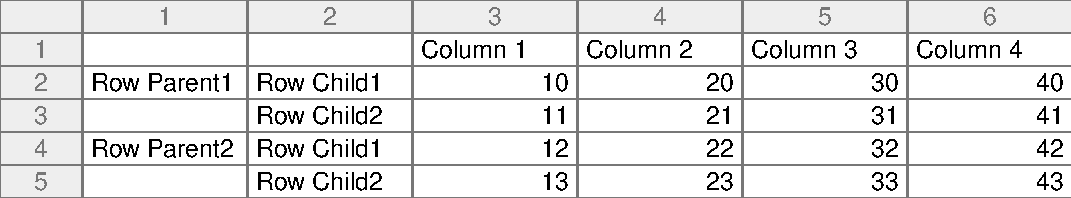
\includegraphics[width=\textwidth]{./TestCase/ToyExByEmptyBelow.pdf}
\end{figure}
\begin{verbatim}
> rowData 
[1] 2 5
> colData 
[1] 3 6
> rowslist 
$label
[1] 1

$data
[1] 2 3 4 5

> colslist 
$label
[1] 1 2

$data
[1] 3 4 5 6

> res 
$`Row Parent1`
$`Row Parent1`$rows
[1] 1 2

$`Row Parent1`$cols
[1] 2


$`Row Parent2`
$`Row Parent2`$rows
[1] 3 4

$`Row Parent2`$cols
[1] 2


> plist 
$rows
[1] 1 2

$cols
[1] 2

> res 
Row Child1 Row Child2 
         1          2 
> plist 
$rows
[1] 3 4

$cols
[1] 2

> res 
Row Child1 Row Child2 
         3          4 
> rowplist 
$`Row Parent1`
+ Row Child1 (1, 2)
+ Row Child2 (2, 2)

$`Row Parent2`
+ Row Child1 (3, 2)
+ Row Child2 (4, 2)

> rowvecs 
     [,1]          [,2]        
[1,] "Row Parent1" "Row Child1"
[2,] "Row Parent1" "Row Child2"
[3,] "Row Parent2" "Row Child1"
[4,] "Row Parent2" "Row Child2"
> matColLabel 
     V3         V4         V5         V6        
[1,] "Column 1" "Column 2" "Column 3" "Column 4"
> cursub 
        V3         V4         V5         V6 
"Column 1" "Column 2" "Column 3" "Column 4" 
> currow[curcols] 
        V3         V4         V5         V6 
"Column 1" "Column 2" "Column 3" "Column 4" 
> matColLabel 
     V3         V4         V5         V6        
[1,] "Column 1" "Column 2" "Column 3" "Column 4"
> matColLabel 
     V3         V4         V5         V6        
[1,] "Column 1" "Column 2" "Column 3" "Column 4"
> matColLabel 
     V3         V4         V5         V6        
[1,] "Column 1" "Column 2" "Column 3" "Column 4"
> plist 
$rows
[1] 1 2 3 4

$cols
[1] 1

> res 
Column 1 Column 2 Column 3 Column 4 
       1        2        3        4 
> plist 
Column 1 Column 2 Column 3 Column 4 
       1        2        3        4 
> matData 
     V3   V4   V5   V6  
[1,] "10" "20" "30" "40"
[2,] "11" "21" "31" "41"
[3,] "12" "22" "32" "42"
[4,] "13" "23" "33" "43"
> datbit 
     V3   V4   V5   V6  
[1,] "10" "20" "30" "40"
[2,] "11" "21" "31" "41"
[3,] "12" "22" "32" "42"
[4,] "13" "23" "33" "43"
> colplist 
Column 1 Column 2 Column 3 Column 4 
       1        2        3        4 
> res 
      UNKNOWN    UNKNOWN Column 1 Column 2 Column 3 Column 4
1 Row Parent1 Row Child1       10       20       30       40
2 Row Parent1 Row Child2       11       21       31       41
3 Row Parent2 Row Child1       12       22       32       42
4 Row Parent2 Row Child2       13       23       33       43
\end{verbatim}

\newpage
\subsection{ToyExByEmptyBelowT.csv}
\label{sec:TCRO_ToyExByEmptyBelowT.csv}
\begin{figure}[!h]
\centering
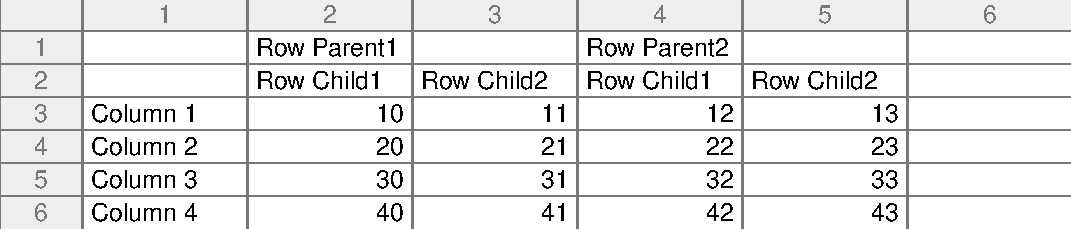
\includegraphics[width=\textwidth]{./TestCase/ToyExByEmptyBelowT.pdf}
\end{figure}
\begin{verbatim}
> rowData 
[1] 3 6
> colData 
[1] 2 5
> rowslist 
$label
[1] 1 2

$data
[1] 3 4 5 6

> colslist 
$label
[1] 1

$data
[1] 2 3 4 5

> plist 
$rows
[1] 1 2 3 4

$cols
[1] 1

> res 
Column 1 Column 2 Column 3 Column 4 
       1        2        3        4 
> rowplist 
Column 1 Column 2 Column 3 Column 4 
       1        2        3        4 
> rowvecs 
     [,1]      
[1,] "Column 1"
[2,] "Column 2"
[3,] "Column 3"
[4,] "Column 4"
> matColLabel 
     V2            V3           V4            V5          
[1,] "Row Parent1" NA           "Row Parent2" NA          
[2,] "Row Child1"  "Row Child2" "Row Child1"  "Row Child2"
> cursub 
           V2            V3 
"Row Parent1"            NA 
> currow[curcols] 
           V2            V3 
"Row Parent1"            NA 
> cursub 
           V4            V5 
"Row Parent2"            NA 
> currow[curcols] 
           V4            V5 
"Row Parent2"            NA 
> cursub 
          V2           V3 
"Row Child1" "Row Child2" 
> currow[curcols] 
          V2           V3 
"Row Child1" "Row Child2" 
> cursub 
          V4           V5 
"Row Child1" "Row Child2" 
> currow[curcols] 
          V4           V5 
"Row Child1" "Row Child2" 
> matColLabel 
     V2            V3           V4            V5          
[1,] "Row Parent1" NA           "Row Parent2" NA          
[2,] "Row Child1"  "Row Child2" "Row Child1"  "Row Child2"
> matColLabel 
     V2            V3           V4            V5          
[1,] "Row Parent1" NA           "Row Parent2" NA          
[2,] "Row Child1"  "Row Child2" "Row Child1"  "Row Child2"
> matColLabel 
     V2            V3           V4            V5          
[1,] "Row Parent1" NA           "Row Parent2" NA          
[2,] "Row Child1"  "Row Child2" "Row Child1"  "Row Child2"
> res 
$`Row Parent1`
$`Row Parent1`$rows
[1] 1 2

$`Row Parent1`$cols
[1] 2


$`Row Parent2`
$`Row Parent2`$rows
[1] 3 4

$`Row Parent2`$cols
[1] 2


> plist 
$rows
[1] 1 2

$cols
[1] 2

> res 
Row Child1 Row Child2 
         1          2 
> plist 
$rows
[1] 3 4

$cols
[1] 2

> res 
Row Child1 Row Child2 
         3          4 
> plist 
Row Child1 Row Child2 
         1          2 
> matData 
     V2   V3   V4   V5  
[1,] "10" "11" "12" "13"
[2,] "20" "21" "22" "23"
[3,] "30" "31" "32" "33"
[4,] "40" "41" "42" "43"
> datbit 
     V2   V3  
[1,] "10" "11"
[2,] "20" "21"
[3,] "30" "31"
[4,] "40" "41"
> plist 
Row Child1 Row Child2 
         3          4 
> matData 
     V2   V3   V4   V5  
[1,] "10" "11" "12" "13"
[2,] "20" "21" "22" "23"
[3,] "30" "31" "32" "33"
[4,] "40" "41" "42" "43"
> datbit 
     V4   V5  
[1,] "12" "13"
[2,] "22" "23"
[3,] "32" "33"
[4,] "42" "43"
> colplist 
$`Row Parent1`
+ Row Child1 (1, 2)
+ Row Child2 (2, 2)

$`Row Parent2`
+ Row Child1 (3, 2)
+ Row Child2 (4, 2)

> res 
      UNKNOWN  UNKNOWN Row Child1 Row Child2
1 Row Parent1 Column 1         10         11
2 Row Parent1 Column 2         20         21
3 Row Parent1 Column 3         30         31
4 Row Parent1 Column 4         40         41
5 Row Parent2 Column 1         12         13
6 Row Parent2 Column 2         22         23
\end{verbatim}

\newpage
\subsection{ToyExByEmptyRight1.csv}
\label{sec:TCRO_ToyExByEmptyRight1.csv}
\begin{figure}[!h]
\centering
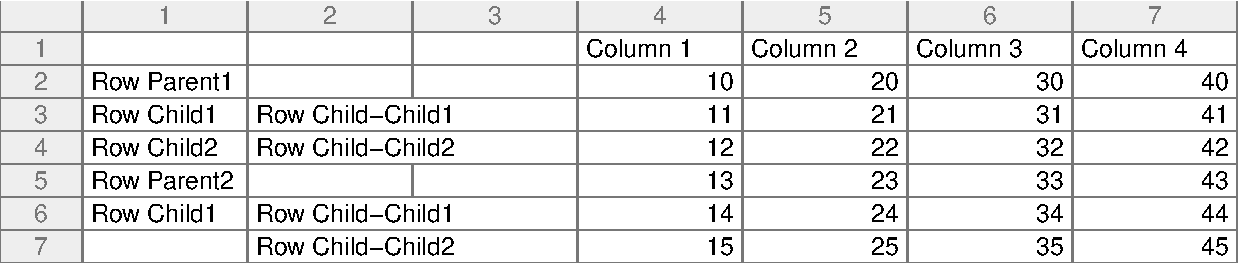
\includegraphics[width=\textwidth]{./TestCase/ToyExByEmptyRight1.pdf}
\end{figure}
\begin{verbatim}
> rowData 
[1] 2 7
> colData 
[1] 4 7
> rowslist 
$label
[1] 1

$data
[1] 2 3 4 5 6 7

> colslist 
$label
[1] 1 2

$data
[1] 4 5 6 7

> res 
$`Row Parent1`
$`Row Parent1`$rows
[1] 2 3

$`Row Parent1`$cols
[1] 1 2


$`Row Parent2`
$`Row Parent2`$rows
[1] 5 6

$`Row Parent2`$cols
[1] 1 2


> res 
$`Row Child1`
$`Row Child1`$rows
[1] 2

$`Row Child1`$cols
[1] 2


$`Row Child2`
$`Row Child2`$rows
[1] 3

$`Row Child2`$cols
[1] 2


> plist 
$rows
[1] 2

$cols
[1] 2

> res 
Row Child-Child1 
               2 
> plist 
$rows
[1] 3

$cols
[1] 2

> res 
Row Child-Child2 
               3 
> res 
$`Row Child1`
$`Row Child1`$rows
[1] 5 6

$`Row Child1`$cols
[1] 2


> plist 
$rows
[1] 5 6

$cols
[1] 2

> res 
Row Child-Child1 Row Child-Child2 
               5                6 
> rowplist 
$`Row Parent1`
+ Row Child1 (2, 1)
- + Row Child-Child1 (2, 2)
+ Row Child2 (3, 1)
- + Row Child-Child2 (3, 2)

$`Row Parent2`
+ Row Child1 (5, 1)
- + Row Child-Child1 (5, 2)
- + Row Child-Child2 (6, 2)

> rowvecs 
   [,1]          [,2]         [,3]              
V2 "Row Parent1" "Row Child1" "Row Child-Child1"
V2 "Row Parent1" "Row Child2" "Row Child-Child2"
   "Row Parent2" "Row Child1" "Row Child-Child1"
   "Row Parent2" "Row Child1" "Row Child-Child2"
> matColLabel 
     V4         V5         V6         V7        
[1,] "Column 1" "Column 2" "Column 3" "Column 4"
> cursub 
        V4         V5         V6         V7 
"Column 1" "Column 2" "Column 3" "Column 4" 
> currow[curcols] 
        V4         V5         V6         V7 
"Column 1" "Column 2" "Column 3" "Column 4" 
> matColLabel 
     V4         V5         V6         V7        
[1,] "Column 1" "Column 2" "Column 3" "Column 4"
> matColLabel 
     V4         V5         V6         V7        
[1,] "Column 1" "Column 2" "Column 3" "Column 4"
> matColLabel 
     V4         V5         V6         V7        
[1,] "Column 1" "Column 2" "Column 3" "Column 4"
> plist 
$rows
[1] 1 2 3 4

$cols
[1] 1

> res 
Column 1 Column 2 Column 3 Column 4 
       1        2        3        4 
> plist 
Column 1 Column 2 Column 3 Column 4 
       1        2        3        4 
> matData 
     V4   V5   V6   V7  
[1,] "11" "21" "31" "41"
[2,] "12" "22" "32" "42"
[3,] "14" "24" "34" "44"
[4,] "15" "25" "35" "45"
> datbit 
     V4   V5   V6   V7  
[1,] "11" "21" "31" "41"
[2,] "12" "22" "32" "42"
[3,] "14" "24" "34" "44"
[4,] "15" "25" "35" "45"
> colplist 
Column 1 Column 2 Column 3 Column 4 
       1        2        3        4 
> res 
      UNKNOWN    UNKNOWN          UNKNOWN Column 1 Column 2 Column 3 Column 4
1 Row Parent1 Row Child1 Row Child-Child1       11       21       31       41
2 Row Parent1 Row Child2 Row Child-Child2       12       22       32       42
3 Row Parent2 Row Child1 Row Child-Child1       14       24       34       44
4 Row Parent2 Row Child1 Row Child-Child2       15       25       35       45
\end{verbatim}

\newpage
\subsection{ToyExByEmptyRight2.csv}
\label{sec:TCRO_ToyExByEmptyRight2.csv}
\begin{figure}[!h]
\centering
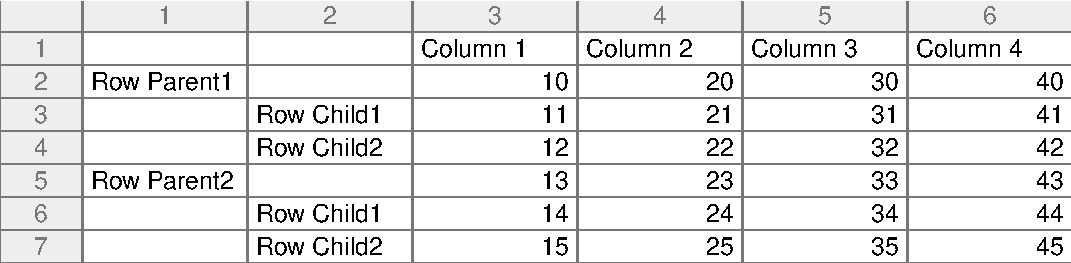
\includegraphics[width=\textwidth]{./TestCase/ToyExByEmptyRight2.pdf}
\end{figure}
\begin{verbatim}
> rowData 
[1] 2 7
> colData 
[1] 3 6
> rowslist 
$label
[1] 1

$data
[1] 2 3 4 5 6 7

> colslist 
$label
[1] 1 2

$data
[1] 3 4 5 6

> res 
$`Row Parent1`
$`Row Parent1`$rows
[1] 2 3

$`Row Parent1`$cols
[1] 1 2


$`Row Parent2`
$`Row Parent2`$rows
[1] 5 6

$`Row Parent2`$cols
[1] 1 2


> plist 
$rows
[1] 2 3

$cols
[1] 2

> res 
Row Child1 Row Child2 
         2          3 
> plist 
$rows
[1] 5 6

$cols
[1] 2

> res 
Row Child1 Row Child2 
         5          6 
> rowplist 
$`Row Parent1`
+ Row Child1 (2, 2)
+ Row Child2 (3, 2)

$`Row Parent2`
+ Row Child1 (5, 2)
+ Row Child2 (6, 2)

> rowvecs 
     [,1]          [,2]        
[1,] "Row Parent1" "Row Child1"
[2,] "Row Parent1" "Row Child2"
[3,] "Row Parent2" "Row Child1"
[4,] "Row Parent2" "Row Child2"
> matColLabel 
     V3         V4         V5         V6        
[1,] "Column 1" "Column 2" "Column 3" "Column 4"
> cursub 
        V3         V4         V5         V6 
"Column 1" "Column 2" "Column 3" "Column 4" 
> currow[curcols] 
        V3         V4         V5         V6 
"Column 1" "Column 2" "Column 3" "Column 4" 
> matColLabel 
     V3         V4         V5         V6        
[1,] "Column 1" "Column 2" "Column 3" "Column 4"
> matColLabel 
     V3         V4         V5         V6        
[1,] "Column 1" "Column 2" "Column 3" "Column 4"
> matColLabel 
     V3         V4         V5         V6        
[1,] "Column 1" "Column 2" "Column 3" "Column 4"
> plist 
$rows
[1] 1 2 3 4

$cols
[1] 1

> res 
Column 1 Column 2 Column 3 Column 4 
       1        2        3        4 
> plist 
Column 1 Column 2 Column 3 Column 4 
       1        2        3        4 
> matData 
     V3   V4   V5   V6  
[1,] "11" "21" "31" "41"
[2,] "12" "22" "32" "42"
[3,] "14" "24" "34" "44"
[4,] "15" "25" "35" "45"
> datbit 
     V3   V4   V5   V6  
[1,] "11" "21" "31" "41"
[2,] "12" "22" "32" "42"
[3,] "14" "24" "34" "44"
[4,] "15" "25" "35" "45"
> colplist 
Column 1 Column 2 Column 3 Column 4 
       1        2        3        4 
> res 
      UNKNOWN    UNKNOWN Column 1 Column 2 Column 3 Column 4
1 Row Parent1 Row Child1       11       21       31       41
2 Row Parent1 Row Child2       12       22       32       42
3 Row Parent2 Row Child1       14       24       34       44
4 Row Parent2 Row Child2       15       25       35       45
\end{verbatim}

\newpage
\subsection{ToyExByEmptyRight3.csv}
\label{sec:TCRO_ToyExByEmptyRight3.csv}
\begin{figure}[!h]
\centering
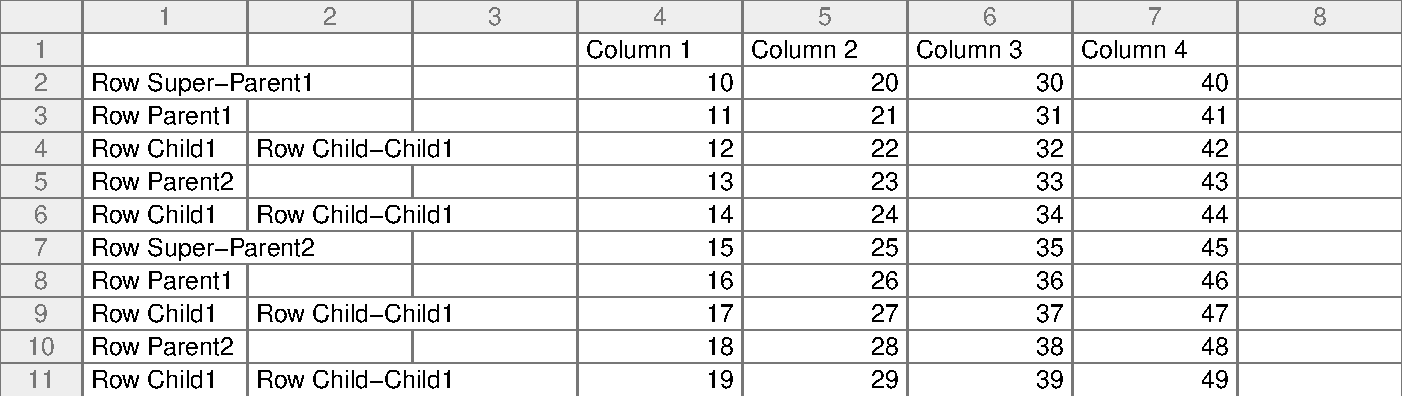
\includegraphics[width=\textwidth]{./TestCase/ToyExByEmptyRight3.pdf}
\end{figure}
\begin{verbatim}
> rowData 
[1]  2 11
> colData 
[1] 4 7
> rowslist 
$label
[1] 1

$data
 [1]  2  3  4  5  6  7  8  9 10 11

> colslist 
$label
[1] 1 2

$data
[1] 4 5 6 7

> res 
$`Row Super-Parent1`
$`Row Super-Parent1`$rows
[1] 2 3 4 5

$`Row Super-Parent1`$cols
[1] 1 2


$`Row Super-Parent2`
$`Row Super-Parent2`$rows
[1]  7  8  9 10

$`Row Super-Parent2`$cols
[1] 1 2


> res 
$`Row Parent1`
$`Row Parent1`$rows
[1] 3

$`Row Parent1`$cols
[1] 1 2


$`Row Parent2`
$`Row Parent2`$rows
[1] 5

$`Row Parent2`$cols
[1] 1 2


> plist 
$rows
[1] 3

$cols
[1] 1 2

> res 
$`Row Child1`
+ Row Child-Child1 (3, 2)

> plist 
$rows
[1] 5

$cols
[1] 1 2

> res 
$`Row Child1`
+ Row Child-Child1 (5, 2)

> res 
$`Row Parent1`
$`Row Parent1`$rows
[1] 8

$`Row Parent1`$cols
[1] 1 2


$`Row Parent2`
$`Row Parent2`$rows
[1] 10

$`Row Parent2`$cols
[1] 1 2


> plist 
$rows
[1] 8

$cols
[1] 1 2

> res 
$`Row Child1`
+ Row Child-Child1 (8, 2)

> plist 
$rows
[1] 10

$cols
[1] 1 2

> res 
$`Row Child1`
+ Row Child-Child1 (10, 2)

> rowplist 
$`Row Super-Parent1`
+ Row Parent1 (2, 1)
- + Row Child1 (3, 1)
- - + Row Child-Child1 (3, 2)
+ Row Parent2 (4, 1)
- + Row Child1 (5, 1)
- - + Row Child-Child1 (5, 2)

$`Row Super-Parent2`
+ Row Parent1 (7, 1)
- + Row Child1 (8, 1)
- - + Row Child-Child1 (8, 2)
+ Row Parent2 (9, 1)
- + Row Child1 (10, 1)
- - + Row Child-Child1 (10, 2)

> rowvecs 
   [,1]                [,2]          [,3]         [,4]              
V2 "Row Super-Parent1" "Row Parent1" "Row Child1" "Row Child-Child1"
V2 "Row Super-Parent1" "Row Parent2" "Row Child1" "Row Child-Child1"
V2 "Row Super-Parent2" "Row Parent1" "Row Child1" "Row Child-Child1"
V2 "Row Super-Parent2" "Row Parent2" "Row Child1" "Row Child-Child1"
> matColLabel 
     V4         V5         V6         V7        
[1,] "Column 1" "Column 2" "Column 3" "Column 4"
> cursub 
        V4         V5         V6         V7 
"Column 1" "Column 2" "Column 3" "Column 4" 
> currow[curcols] 
        V4         V5         V6         V7 
"Column 1" "Column 2" "Column 3" "Column 4" 
> matColLabel 
     V4         V5         V6         V7        
[1,] "Column 1" "Column 2" "Column 3" "Column 4"
> matColLabel 
     V4         V5         V6         V7        
[1,] "Column 1" "Column 2" "Column 3" "Column 4"
> matColLabel 
     V4         V5         V6         V7        
[1,] "Column 1" "Column 2" "Column 3" "Column 4"
> plist 
$rows
[1] 1 2 3 4

$cols
[1] 1

> res 
Column 1 Column 2 Column 3 Column 4 
       1        2        3        4 
> plist 
Column 1 Column 2 Column 3 Column 4 
       1        2        3        4 
> matData 
     V4   V5   V6   V7  
[1,] "12" "22" "32" "42"
[2,] "14" "24" "34" "44"
[3,] "17" "27" "37" "47"
[4,] "19" "29" "39" "49"
> datbit 
     V4   V5   V6   V7  
[1,] "12" "22" "32" "42"
[2,] "14" "24" "34" "44"
[3,] "17" "27" "37" "47"
[4,] "19" "29" "39" "49"
> colplist 
Column 1 Column 2 Column 3 Column 4 
       1        2        3        4 
> res 
            UNKNOWN     UNKNOWN    UNKNOWN          UNKNOWN Column 1 Column 2
1 Row Super-Parent1 Row Parent1 Row Child1 Row Child-Child1       12       22
2 Row Super-Parent1 Row Parent2 Row Child1 Row Child-Child1       14       24
3 Row Super-Parent2 Row Parent1 Row Child1 Row Child-Child1       17       27
4 Row Super-Parent2 Row Parent2 Row Child1 Row Child-Child1       19       29
  Column 3 Column 4
1       32       42
2       34       44
3       37       47
4       39       49
\end{verbatim}

\newpage
\subsection{ToyExComplete.csv}
\label{sec:TCRO_ToyExComplete.csv}
\begin{figure}[!h]
\centering
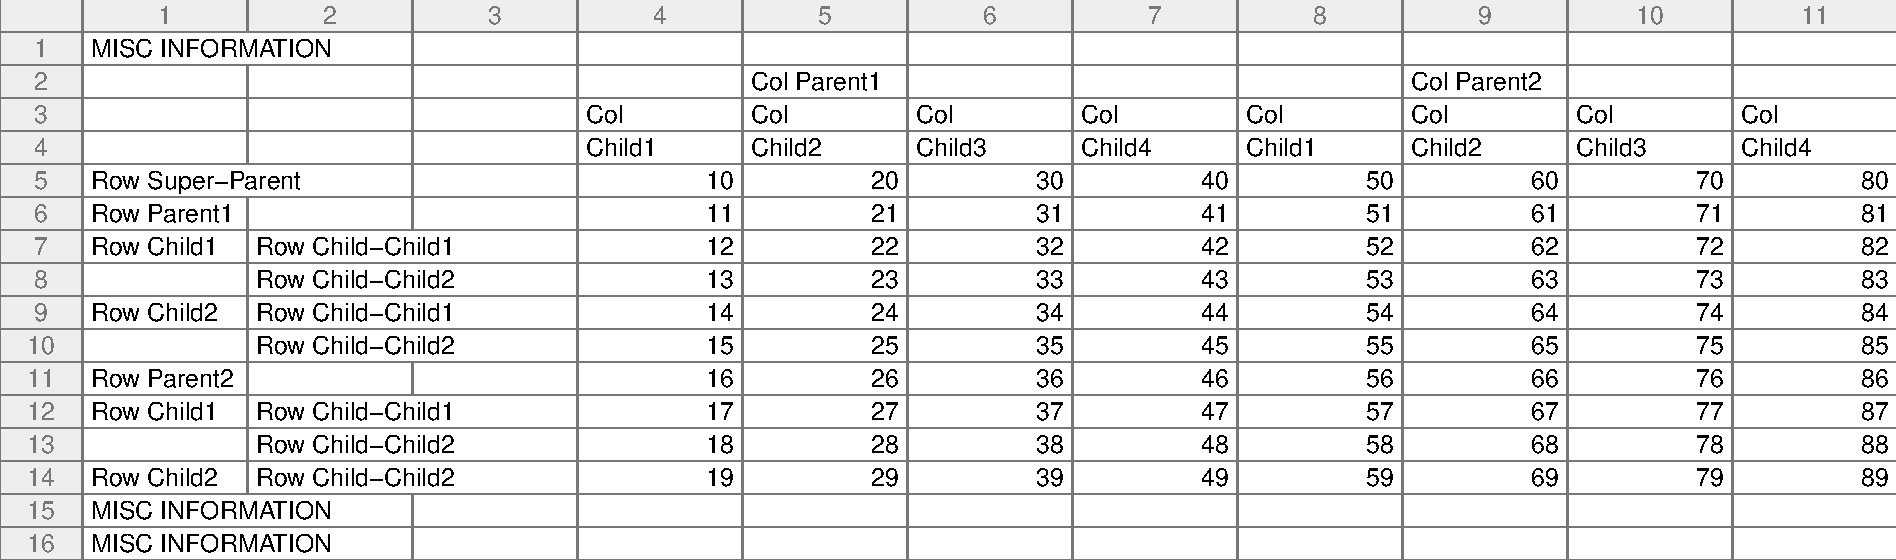
\includegraphics[width=\textwidth]{./TestCase/ToyExComplete.pdf}
\end{figure}
\begin{verbatim}
> rowData 
[1]  5 14
> colData 
[1]  4 11
> rowslist 
$label
[1] 1 2 3 4

$data
 [1]  5  6  7  8  9 10 11 12 13 14

> colslist 
$label
[1] 1 2

$data
[1]  4  5  6  7  8  9 10 11

> res 
$`Row Super-Parent`
$`Row Super-Parent`$rows
[1]  2  3  4  5  6  7  8  9 10

$`Row Super-Parent`$cols
[1] 1 2


> res 
$`Row Parent1`
$`Row Parent1`$rows
[1] 3 4 5 6

$`Row Parent1`$cols
[1] 1 2


$`Row Parent2`
$`Row Parent2`$rows
[1]  8  9 10

$`Row Parent2`$cols
[1] 1 2


> res 
$`Row Child1`
$`Row Child1`$rows
[1] 3 4

$`Row Child1`$cols
[1] 2


$`Row Child2`
$`Row Child2`$rows
[1] 5 6

$`Row Child2`$cols
[1] 2


> plist 
$rows
[1] 3 4

$cols
[1] 2

> res 
Row Child-Child1 Row Child-Child2 
               3                4 
> plist 
$rows
[1] 5 6

$cols
[1] 2

> res 
Row Child-Child1 Row Child-Child2 
               5                6 
> res 
$`Row Child1`
$`Row Child1`$rows
[1] 8 9

$`Row Child1`$cols
[1] 2


$`Row Child2`
$`Row Child2`$rows
[1] 10

$`Row Child2`$cols
[1] 2


> plist 
$rows
[1] 8 9

$cols
[1] 2

> res 
Row Child-Child1 Row Child-Child2 
               8                9 
> plist 
$rows
[1] 10

$cols
[1] 2

> res 
Row Child-Child2 
              10 
> rowplist 
$`Row Super-Parent`
+ Row Parent1 (2, 1)
- + Row Child1 (3, 1)
- - + Row Child-Child1 (3, 2)
- - + Row Child-Child2 (4, 2)
- + Row Child2 (5, 1)
- - + Row Child-Child1 (5, 2)
- - + Row Child-Child2 (6, 2)
+ Row Parent2 (7, 1)
- + Row Child1 (8, 1)
- - + Row Child-Child1 (8, 2)
- - + Row Child-Child2 (9, 2)
- + Row Child2 (10, 1)
- - + Row Child-Child2 (10, 2)

> rowvecs 
 [,1]               [,2]          [,3]         [,4]              
 "Row Super-Parent" "Row Parent1" "Row Child1" "Row Child-Child1"
 "Row Super-Parent" "Row Parent1" "Row Child1" "Row Child-Child2"
 "Row Super-Parent" "Row Parent1" "Row Child2" "Row Child-Child1"
 "Row Super-Parent" "Row Parent1" "Row Child2" "Row Child-Child2"
 "Row Super-Parent" "Row Parent2" "Row Child1" "Row Child-Child1"
 "Row Super-Parent" "Row Parent2" "Row Child1" "Row Child-Child2"
> matColLabel 
     V4       V5            V6       V7       V8       V9           
[1,] NA       NA            NA       NA       NA       NA           
[2,] NA       "Col Parent1" NA       NA       NA       "Col Parent2"
[3,] "Col"    "Col"         "Col"    "Col"    "Col"    "Col"        
[4,] "Child1" "Child2"      "Child3" "Child4" "Child1" "Child2"     
> cursub 
           V4            V5            V6            V7 
           NA "Col Parent1"            NA            NA 
> currow[curcols] 
           V4            V5            V6            V7 
"Col Parent1"            NA            NA            NA 
> cursub 
           V8            V9           V10           V11 
           NA "Col Parent2"            NA            NA 
> currow[curcols] 
           V8            V9           V10           V11 
"Col Parent2"            NA            NA            NA 
> cursub 
   V4 
"Col" 
> currow[curcols] 
   V4 
"Col" 
> cursub 
   V5 
"Col" 
> currow[curcols] 
   V5 
"Col" 
> cursub 
   V6 
"Col" 
> currow[curcols] 
   V6 
"Col" 
> cursub 
   V7 
"Col" 
> currow[curcols] 
   V7 
"Col" 
> cursub 
   V8 
"Col" 
> currow[curcols] 
   V8 
"Col" 
> cursub 
   V9 
"Col" 
> currow[curcols] 
   V9 
"Col" 
> cursub 
  V10 
"Col" 
> currow[curcols] 
  V10 
"Col" 
> cursub 
  V11 
"Col" 
> currow[curcols] 
  V11 
"Col" 
> cursub 
      V4       V5       V6       V7 
"Child1" "Child2" "Child3" "Child4" 
> currow[curcols] 
      V4       V5       V6       V7 
"Child1" "Child2" "Child3" "Child4" 
> cursub 
      V8       V9      V10      V11 
"Child1" "Child2" "Child3" "Child4" 
> currow[curcols] 
      V8       V9      V10      V11 
"Child1" "Child2" "Child3" "Child4" 
> matColLabel 
     V4            V5       V6       V7       V8            V9      
[1,] NA            NA       NA       NA       NA            NA      
[2,] "Col Parent1" NA       NA       NA       "Col Parent2" NA      
[3,] "Col"         "Col"    "Col"    "Col"    "Col"         "Col"   
[4,] "Child1"      "Child2" "Child3" "Child4" "Child1"      "Child2"
> matColLabel 
     V4            V5       V6       V7       V8            V9      
[1,] NA            NA       NA       NA       NA            NA      
[2,] "Col Parent1" NA       NA       NA       "Col Parent2" NA      
[3,] "Col"         "Col"    "Col"    "Col"    "Col"         "Col"   
[4,] "Child1"      "Child2" "Child3" "Child4" "Child1"      "Child2"
> matColLabel 
     V4            V5           V6           V7           V8           
[1,] NA            NA           NA           NA           NA           
[2,] "Col Parent1" NA           NA           NA           "Col Parent2"
[3,] "Col Child1"  "Col Child2" "Col Child3" "Col Child4" "Col Child1" 
     V9          
[1,] NA          
[2,] NA          
[3,] "Col Child2"
> res 
$`Col Parent1`
$`Col Parent1`$rows
[1] 1 2 3 4

$`Col Parent1`$cols
[1] 3


$`Col Parent2`
$`Col Parent2`$rows
[1] 5 6 7 8

$`Col Parent2`$cols
[1] 3


> plist 
$rows
[1] 1 2 3 4

$cols
[1] 3

> res 
Col Child1 Col Child2 Col Child3 Col Child4 
         1          2          3          4 
> plist 
$rows
[1] 5 6 7 8

$cols
[1] 3

> res 
Col Child1 Col Child2 Col Child3 Col Child4 
         5          6          7          8 
> plist 
Col Child1 Col Child2 Col Child3 Col Child4 
         1          2          3          4 
> matData 
     V4   V5   V6   V7   V8   V9  
[1,] "12" "22" "32" "42" "52" "62"
[2,] "13" "23" "33" "43" "53" "63"
[3,] "14" "24" "34" "44" "54" "64"
[4,] "15" "25" "35" "45" "55" "65"
[5,] "17" "27" "37" "47" "57" "67"
[6,] "18" "28" "38" "48" "58" "68"
> datbit 
     V4   V5   V6   V7  
[1,] "12" "22" "32" "42"
[2,] "13" "23" "33" "43"
[3,] "14" "24" "34" "44"
[4,] "15" "25" "35" "45"
[5,] "17" "27" "37" "47"
[6,] "18" "28" "38" "48"
> plist 
Col Child1 Col Child2 Col Child3 Col Child4 
         5          6          7          8 
> matData 
     V4   V5   V6   V7   V8   V9  
[1,] "12" "22" "32" "42" "52" "62"
[2,] "13" "23" "33" "43" "53" "63"
[3,] "14" "24" "34" "44" "54" "64"
[4,] "15" "25" "35" "45" "55" "65"
[5,] "17" "27" "37" "47" "57" "67"
[6,] "18" "28" "38" "48" "58" "68"
> datbit 
     V8   V9   V10  V11 
[1,] "52" "62" "72" "82"
[2,] "53" "63" "73" "83"
[3,] "54" "64" "74" "84"
[4,] "55" "65" "75" "85"
[5,] "57" "67" "77" "87"
[6,] "58" "68" "78" "88"
> colplist 
$`Col Parent1`
+ Col Child1 (1, 3)
+ Col Child2 (2, 3)
+ Col Child3 (3, 3)
+ Col Child4 (4, 3)

$`Col Parent2`
+ Col Child1 (5, 3)
+ Col Child2 (6, 3)
+ Col Child3 (7, 3)
+ Col Child4 (8, 3)

> res 
      UNKNOWN          UNKNOWN     UNKNOWN    UNKNOWN          UNKNOWN
1 Col Parent1 Row Super-Parent Row Parent1 Row Child1 Row Child-Child1
2 Col Parent1 Row Super-Parent Row Parent1 Row Child1 Row Child-Child2
3 Col Parent1 Row Super-Parent Row Parent1 Row Child2 Row Child-Child1
4 Col Parent1 Row Super-Parent Row Parent1 Row Child2 Row Child-Child2
5 Col Parent1 Row Super-Parent Row Parent2 Row Child1 Row Child-Child1
6 Col Parent1 Row Super-Parent Row Parent2 Row Child1 Row Child-Child2
  Col Child1 Col Child2 Col Child3 Col Child4
1         12         22         32         42
2         13         23         33         43
3         14         24         34         44
4         15         25         35         45
5         17         27         37         47
6         18         28         38         48
\end{verbatim}

\newpage
\subsection{ToyExFindSingleTable.csv}
\label{sec:TCRO_ToyExFindSingleTable.csv}
\begin{figure}[!h]
\centering
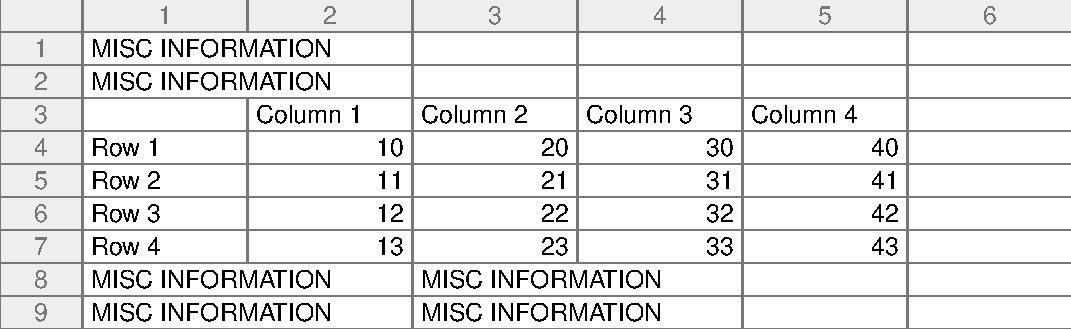
\includegraphics[width=\textwidth]{./TestCase/ToyExFindSingleTable.pdf}
\end{figure}
\begin{verbatim}
> rowData 
[1] 4 7
> colData 
[1] 2 5
> rowslist 
$label
[1] 1 2 3

$data
[1] 4 5 6 7

> colslist 
$label
[1] 1

$data
[1] 2 3 4 5

> plist 
$rows
[1] 1 2 3 4

$cols
[1] 1

> res 
Row 1 Row 2 Row 3 Row 4 
    1     2     3     4 
> rowplist 
Row 1 Row 2 Row 3 Row 4 
    1     2     3     4 
> rowvecs 
     [,1]   
[1,] "Row 1"
[2,] "Row 2"
[3,] "Row 3"
[4,] "Row 4"
> matColLabel 
     V2         V3         V4         V5        
[1,] NA         NA         NA         NA        
[2,] NA         NA         NA         NA        
[3,] "Column 1" "Column 2" "Column 3" "Column 4"
> cursub 
        V2         V3         V4         V5 
"Column 1" "Column 2" "Column 3" "Column 4" 
> currow[curcols] 
        V2         V3         V4         V5 
"Column 1" "Column 2" "Column 3" "Column 4" 
> matColLabel 
     V2         V3         V4         V5        
[1,] NA         NA         NA         NA        
[2,] NA         NA         NA         NA        
[3,] "Column 1" "Column 2" "Column 3" "Column 4"
> matColLabel 
     V2         V3         V4         V5        
[1,] NA         NA         NA         NA        
[2,] NA         NA         NA         NA        
[3,] "Column 1" "Column 2" "Column 3" "Column 4"
> matColLabel 
     V2         V3         V4         V5        
[1,] NA         NA         NA         NA        
[2,] NA         NA         NA         NA        
[3,] "Column 1" "Column 2" "Column 3" "Column 4"
> plist 
$rows
[1] 1 2 3 4

$cols
[1] 3

> res 
Column 1 Column 2 Column 3 Column 4 
       1        2        3        4 
> plist 
Column 1 Column 2 Column 3 Column 4 
       1        2        3        4 
> matData 
     V2   V3   V4   V5  
[1,] "10" "20" "30" "40"
[2,] "11" "21" "31" "41"
[3,] "12" "22" "32" "42"
[4,] "13" "23" "33" "43"
> datbit 
     V2   V3   V4   V5  
[1,] "10" "20" "30" "40"
[2,] "11" "21" "31" "41"
[3,] "12" "22" "32" "42"
[4,] "13" "23" "33" "43"
> colplist 
Column 1 Column 2 Column 3 Column 4 
       1        2        3        4 
> res 
  UNKNOWN Column 1 Column 2 Column 3 Column 4
1   Row 1       10       20       30       40
2   Row 2       11       21       31       41
3   Row 3       12       22       32       42
4   Row 4       13       23       33       43
\end{verbatim}

\newpage
\subsection{ToyExIrregularColumnLabels.csv}
\label{sec:TCRO_ToyExIrregularColumnLabels.csv}
\begin{figure}[!h]
\centering
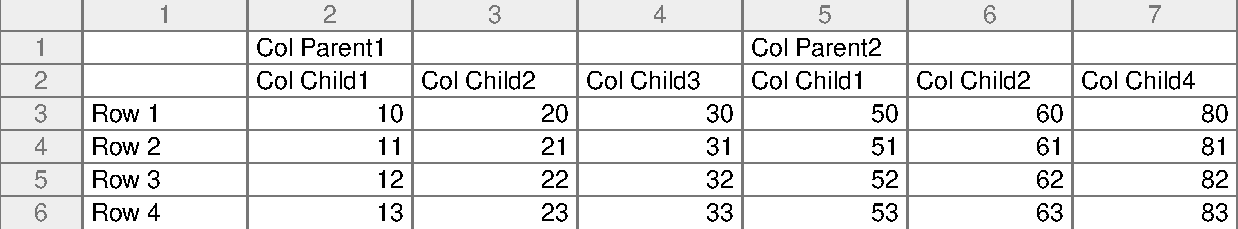
\includegraphics[width=\textwidth]{./TestCase/ToyExIrregularColumnLabels.pdf}
\end{figure}
\begin{verbatim}
> rowData 
[1] 3 6
> colData 
[1] 2 7
> rowslist 
$label
[1] 1 2

$data
[1] 3 4 5 6

> colslist 
$label
[1] 1

$data
[1] 2 3 4 5 6 7

> plist 
$rows
[1] 1 2 3 4

$cols
[1] 1

> res 
Row 1 Row 2 Row 3 Row 4 
    1     2     3     4 
> rowplist 
Row 1 Row 2 Row 3 Row 4 
    1     2     3     4 
> rowvecs 
     [,1]   
[1,] "Row 1"
[2,] "Row 2"
[3,] "Row 3"
[4,] "Row 4"
> matColLabel 
     V2            V3           V4           V5            V6          
[1,] "Col Parent1" NA           NA           "Col Parent2" NA          
[2,] "Col Child1"  "Col Child2" "Col Child3" "Col Child1"  "Col Child2"
     V7          
[1,] NA          
[2,] "Col Child4"
> cursub 
           V2            V3            V4 
"Col Parent1"            NA            NA 
> currow[curcols] 
           V2            V3            V4 
"Col Parent1"            NA            NA 
> cursub 
           V5            V6            V7 
"Col Parent2"            NA            NA 
> currow[curcols] 
           V5            V6            V7 
"Col Parent2"            NA            NA 
> cursub 
          V2           V3           V4           V5           V6           V7 
"Col Child1" "Col Child2" "Col Child3" "Col Child1" "Col Child2" "Col Child4" 
> currow[curcols] 
          V2           V3           V4           V5           V6           V7 
"Col Child1" "Col Child2" "Col Child3" "Col Child1" "Col Child2" "Col Child4" 
> matColLabel 
     V2            V3           V4           V5            V6          
[1,] "Col Parent1" NA           NA           "Col Parent2" NA          
[2,] "Col Child1"  "Col Child2" "Col Child3" "Col Child1"  "Col Child2"
     V7          
[1,] NA          
[2,] "Col Child4"
> matColLabel 
     V2            V3           V4           V5            V6          
[1,] "Col Parent1" NA           NA           "Col Parent2" NA          
[2,] "Col Child1"  "Col Child2" "Col Child3" "Col Child1"  "Col Child2"
     V7          
[1,] NA          
[2,] "Col Child4"
> matColLabel 
     V2            V3           V4           V5            V6          
[1,] "Col Parent1" NA           NA           "Col Parent2" NA          
[2,] "Col Child1"  "Col Child2" "Col Child3" "Col Child1"  "Col Child2"
     V7          
[1,] NA          
[2,] "Col Child4"
> res 
$`Col Parent1`
$`Col Parent1`$rows
[1] 1 2 3

$`Col Parent1`$cols
[1] 2


$`Col Parent2`
$`Col Parent2`$rows
[1] 4 5 6

$`Col Parent2`$cols
[1] 2


> plist 
$rows
[1] 1 2 3

$cols
[1] 2

> res 
Col Child1 Col Child2 Col Child3 
         1          2          3 
> plist 
$rows
[1] 4 5 6

$cols
[1] 2

> res 
Col Child1 Col Child2 Col Child4 
         4          5          6 
> plist 
Col Child1 Col Child2 Col Child3 
         1          2          3 
> matData 
     V2   V3   V4   V5   V6   V7  
[1,] "10" "20" "30" "50" "60" "80"
[2,] "11" "21" "31" "51" "61" "81"
[3,] "12" "22" "32" "52" "62" "82"
[4,] "13" "23" "33" "53" "63" "83"
> datbit 
     V2   V3   V4  
[1,] "10" "20" "30"
[2,] "11" "21" "31"
[3,] "12" "22" "32"
[4,] "13" "23" "33"
> plist 
Col Child1 Col Child2 Col Child4 
         4          5          6 
> matData 
     V2   V3   V4   V5   V6   V7  
[1,] "10" "20" "30" "50" "60" "80"
[2,] "11" "21" "31" "51" "61" "81"
[3,] "12" "22" "32" "52" "62" "82"
[4,] "13" "23" "33" "53" "63" "83"
> datbit 
     V5   V6   V7  
[1,] "50" "60" "80"
[2,] "51" "61" "81"
[3,] "52" "62" "82"
[4,] "53" "63" "83"
> colplist 
$`Col Parent1`
+ Col Child1 (1, 2)
+ Col Child2 (2, 2)
+ Col Child3 (3, 2)

$`Col Parent2`
+ Col Child1 (4, 2)
+ Col Child2 (5, 2)
+ Col Child4 (6, 2)

> res 
      UNKNOWN UNKNOWN Col Child1 Col Child2 Col Child3 Col Child4
1 Col Parent1   Row 1         10         20         30         NA
2 Col Parent1   Row 2         11         21         31         NA
3 Col Parent1   Row 3         12         22         32         NA
4 Col Parent1   Row 4         13         23         33         NA
5 Col Parent2   Row 1         50         60         NA         80
6 Col Parent2   Row 2         51         61         NA         81
\end{verbatim}

\newpage
\subsection{ToyExMisalignedColumnLabel.csv}
\label{sec:TCRO_ToyExMisalignedColumnLabel.csv}
\begin{figure}[!h]
\centering
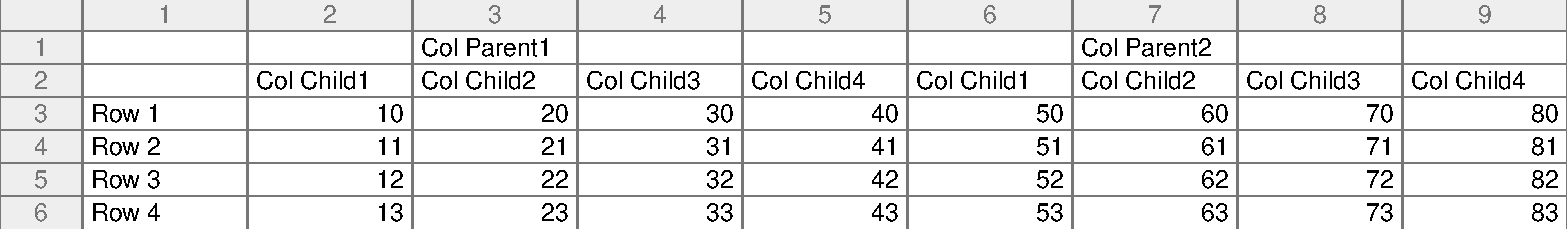
\includegraphics[width=\textwidth]{./TestCase/ToyExMisalignedColumnLabel.pdf}
\end{figure}
\begin{verbatim}
> rowData 
[1] 3 6
> colData 
[1] 2 9
> rowslist 
$label
[1] 1 2

$data
[1] 3 4 5 6

> colslist 
$label
[1] 1

$data
[1] 2 3 4 5 6 7 8 9

> plist 
$rows
[1] 1 2 3 4

$cols
[1] 1

> res 
Row 1 Row 2 Row 3 Row 4 
    1     2     3     4 
> rowplist 
Row 1 Row 2 Row 3 Row 4 
    1     2     3     4 
> rowvecs 
     [,1]   
[1,] "Row 1"
[2,] "Row 2"
[3,] "Row 3"
[4,] "Row 4"
> matColLabel 
     V2           V3            V4           V5           V6          
[1,] NA           "Col Parent1" NA           NA           NA          
[2,] "Col Child1" "Col Child2"  "Col Child3" "Col Child4" "Col Child1"
     V7           
[1,] "Col Parent2"
[2,] "Col Child2" 
> cursub 
           V2            V3            V4            V5 
           NA "Col Parent1"            NA            NA 
> currow[curcols] 
           V2            V3            V4            V5 
"Col Parent1"            NA            NA            NA 
> cursub 
           V6            V7            V8            V9 
           NA "Col Parent2"            NA            NA 
> currow[curcols] 
           V6            V7            V8            V9 
"Col Parent2"            NA            NA            NA 
> cursub 
          V2           V3           V4           V5 
"Col Child1" "Col Child2" "Col Child3" "Col Child4" 
> currow[curcols] 
          V2           V3           V4           V5 
"Col Child1" "Col Child2" "Col Child3" "Col Child4" 
> cursub 
          V6           V7           V8           V9 
"Col Child1" "Col Child2" "Col Child3" "Col Child4" 
> currow[curcols] 
          V6           V7           V8           V9 
"Col Child1" "Col Child2" "Col Child3" "Col Child4" 
> matColLabel 
     V2            V3           V4           V5           V6           
[1,] "Col Parent1" NA           NA           NA           "Col Parent2"
[2,] "Col Child1"  "Col Child2" "Col Child3" "Col Child4" "Col Child1" 
     V7          
[1,] NA          
[2,] "Col Child2"
> matColLabel 
     V2            V3           V4           V5           V6           
[1,] "Col Parent1" NA           NA           NA           "Col Parent2"
[2,] "Col Child1"  "Col Child2" "Col Child3" "Col Child4" "Col Child1" 
     V7          
[1,] NA          
[2,] "Col Child2"
> matColLabel 
     V2            V3           V4           V5           V6           
[1,] "Col Parent1" NA           NA           NA           "Col Parent2"
[2,] "Col Child1"  "Col Child2" "Col Child3" "Col Child4" "Col Child1" 
     V7          
[1,] NA          
[2,] "Col Child2"
> res 
$`Col Parent1`
$`Col Parent1`$rows
[1] 1 2 3 4

$`Col Parent1`$cols
[1] 2


$`Col Parent2`
$`Col Parent2`$rows
[1] 5 6 7 8

$`Col Parent2`$cols
[1] 2


> plist 
$rows
[1] 1 2 3 4

$cols
[1] 2

> res 
Col Child1 Col Child2 Col Child3 Col Child4 
         1          2          3          4 
> plist 
$rows
[1] 5 6 7 8

$cols
[1] 2

> res 
Col Child1 Col Child2 Col Child3 Col Child4 
         5          6          7          8 
> plist 
Col Child1 Col Child2 Col Child3 Col Child4 
         1          2          3          4 
> matData 
     V2   V3   V4   V5   V6   V7  
[1,] "10" "20" "30" "40" "50" "60"
[2,] "11" "21" "31" "41" "51" "61"
[3,] "12" "22" "32" "42" "52" "62"
[4,] "13" "23" "33" "43" "53" "63"
> datbit 
     V2   V3   V4   V5  
[1,] "10" "20" "30" "40"
[2,] "11" "21" "31" "41"
[3,] "12" "22" "32" "42"
[4,] "13" "23" "33" "43"
> plist 
Col Child1 Col Child2 Col Child3 Col Child4 
         5          6          7          8 
> matData 
     V2   V3   V4   V5   V6   V7  
[1,] "10" "20" "30" "40" "50" "60"
[2,] "11" "21" "31" "41" "51" "61"
[3,] "12" "22" "32" "42" "52" "62"
[4,] "13" "23" "33" "43" "53" "63"
> datbit 
     V6   V7   V8   V9  
[1,] "50" "60" "70" "80"
[2,] "51" "61" "71" "81"
[3,] "52" "62" "72" "82"
[4,] "53" "63" "73" "83"
> colplist 
$`Col Parent1`
+ Col Child1 (1, 2)
+ Col Child2 (2, 2)
+ Col Child3 (3, 2)
+ Col Child4 (4, 2)

$`Col Parent2`
+ Col Child1 (5, 2)
+ Col Child2 (6, 2)
+ Col Child3 (7, 2)
+ Col Child4 (8, 2)

> res 
      UNKNOWN UNKNOWN Col Child1 Col Child2 Col Child3 Col Child4
1 Col Parent1   Row 1         10         20         30         40
2 Col Parent1   Row 2         11         21         31         41
3 Col Parent1   Row 3         12         22         32         42
4 Col Parent1   Row 4         13         23         33         43
5 Col Parent2   Row 1         50         60         70         80
6 Col Parent2   Row 2         51         61         71         81
\end{verbatim}

\newpage
\subsection{ToyExMisalignedColumnLabel2.csv}
\label{sec:TCRO_ToyExMisalignedColumnLabel2.csv}
\begin{figure}[!h]
\centering
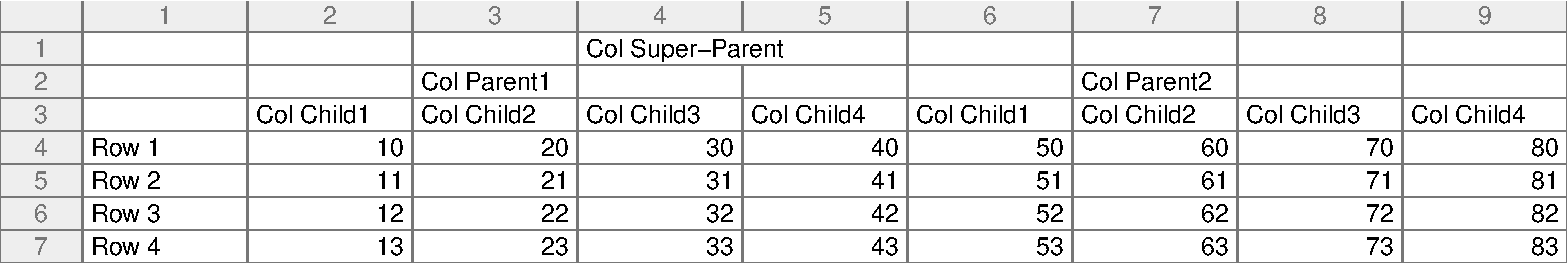
\includegraphics[width=\textwidth]{./TestCase/ToyExMisalignedColumnLabel2.pdf}
\end{figure}
\begin{verbatim}
> rowData 
[1] 4 7
> colData 
[1] 2 9
> rowslist 
$label
[1] 1 2 3

$data
[1] 4 5 6 7

> colslist 
$label
[1] 1

$data
[1] 2 3 4 5 6 7 8 9

> plist 
$rows
[1] 1 2 3 4

$cols
[1] 1

> res 
Row 1 Row 2 Row 3 Row 4 
    1     2     3     4 
> rowplist 
Row 1 Row 2 Row 3 Row 4 
    1     2     3     4 
> rowvecs 
     [,1]   
[1,] "Row 1"
[2,] "Row 2"
[3,] "Row 3"
[4,] "Row 4"
> matColLabel 
     V2           V3            V4                 V5           V6          
[1,] NA           NA            "Col Super-Parent" NA           NA          
[2,] NA           "Col Parent1" NA                 NA           NA          
[3,] "Col Child1" "Col Child2"  "Col Child3"       "Col Child4" "Col Child1"
     V7           
[1,] NA           
[2,] "Col Parent2"
[3,] "Col Child2" 
> cursub 
                V2                 V3                 V4                 V5 
                NA                 NA "Col Super-Parent"                 NA 
                V6                 V7 
                NA                 NA 
> currow[curcols] 
                V2                 V3                 V4                 V5 
"Col Super-Parent"                 NA                 NA                 NA 
                V6                 V7 
                NA                 NA 
> cursub 
           V2            V3            V4            V5 
           NA "Col Parent1"            NA            NA 
> currow[curcols] 
           V2            V3            V4            V5 
"Col Parent1"            NA            NA            NA 
> cursub 
           V6            V7            V8            V9 
           NA "Col Parent2"            NA            NA 
> currow[curcols] 
           V6            V7            V8            V9 
"Col Parent2"            NA            NA            NA 
> cursub 
          V2           V3           V4           V5 
"Col Child1" "Col Child2" "Col Child3" "Col Child4" 
> currow[curcols] 
          V2           V3           V4           V5 
"Col Child1" "Col Child2" "Col Child3" "Col Child4" 
> cursub 
          V6           V7           V8           V9 
"Col Child1" "Col Child2" "Col Child3" "Col Child4" 
> currow[curcols] 
          V6           V7           V8           V9 
"Col Child1" "Col Child2" "Col Child3" "Col Child4" 
> matColLabel 
     V2                 V3           V4           V5           V6           
[1,] "Col Super-Parent" NA           NA           NA           NA           
[2,] "Col Parent1"      NA           NA           NA           "Col Parent2"
[3,] "Col Child1"       "Col Child2" "Col Child3" "Col Child4" "Col Child1" 
     V7          
[1,] NA          
[2,] NA          
[3,] "Col Child2"
> matColLabel 
     V2                 V3           V4           V5           V6           
[1,] "Col Super-Parent" NA           NA           NA           NA           
[2,] "Col Parent1"      NA           NA           NA           "Col Parent2"
[3,] "Col Child1"       "Col Child2" "Col Child3" "Col Child4" "Col Child1" 
     V7          
[1,] NA          
[2,] NA          
[3,] "Col Child2"
> matColLabel 
     V2                 V3           V4           V5           V6           
[1,] "Col Super-Parent" NA           NA           NA           NA           
[2,] "Col Parent1"      NA           NA           NA           "Col Parent2"
[3,] "Col Child1"       "Col Child2" "Col Child3" "Col Child4" "Col Child1" 
     V7          
[1,] NA          
[2,] NA          
[3,] "Col Child2"
> res 
$`Col Super-Parent`
$`Col Super-Parent`$rows
[1] 1 2 3 4 5 6 7 8

$`Col Super-Parent`$cols
[1] 2 3


> res 
$`Col Parent1`
$`Col Parent1`$rows
[1] 1 2 3 4

$`Col Parent1`$cols
[1] 3


$`Col Parent2`
$`Col Parent2`$rows
[1] 5 6 7 8

$`Col Parent2`$cols
[1] 3


> plist 
$rows
[1] 1 2 3 4

$cols
[1] 3

> res 
Col Child1 Col Child2 Col Child3 Col Child4 
         1          2          3          4 
> plist 
$rows
[1] 5 6 7 8

$cols
[1] 3

> res 
Col Child1 Col Child2 Col Child3 Col Child4 
         5          6          7          8 
> plist 
Col Child1 Col Child2 Col Child3 Col Child4 
         1          2          3          4 
> matData 
     V2   V3   V4   V5   V6   V7  
[1,] "10" "20" "30" "40" "50" "60"
[2,] "11" "21" "31" "41" "51" "61"
[3,] "12" "22" "32" "42" "52" "62"
[4,] "13" "23" "33" "43" "53" "63"
> datbit 
     V2   V3   V4   V5  
[1,] "10" "20" "30" "40"
[2,] "11" "21" "31" "41"
[3,] "12" "22" "32" "42"
[4,] "13" "23" "33" "43"
> plist 
Col Child1 Col Child2 Col Child3 Col Child4 
         5          6          7          8 
> matData 
     V2   V3   V4   V5   V6   V7  
[1,] "10" "20" "30" "40" "50" "60"
[2,] "11" "21" "31" "41" "51" "61"
[3,] "12" "22" "32" "42" "52" "62"
[4,] "13" "23" "33" "43" "53" "63"
> datbit 
     V6   V7   V8   V9  
[1,] "50" "60" "70" "80"
[2,] "51" "61" "71" "81"
[3,] "52" "62" "72" "82"
[4,] "53" "63" "73" "83"
> colplist 
$`Col Super-Parent`
+ Col Parent1 (1, 2)
- + Col Child1 (1, 3)
- + Col Child2 (2, 3)
- + Col Child3 (3, 3)
- + Col Child4 (4, 3)
+ Col Parent2 (5, 2)
- + Col Child1 (5, 3)
- + Col Child2 (6, 3)
- + Col Child3 (7, 3)
- + Col Child4 (8, 3)

> res 
           UNKNOWN     UNKNOWN UNKNOWN Col Child1 Col Child2 Col Child3
1 Col Super-Parent Col Parent1   Row 1         10         20         30
2 Col Super-Parent Col Parent1   Row 2         11         21         31
3 Col Super-Parent Col Parent1   Row 3         12         22         32
4 Col Super-Parent Col Parent1   Row 4         13         23         33
5 Col Super-Parent Col Parent2   Row 1         50         60         70
6 Col Super-Parent Col Parent2   Row 2         51         61         71
  Col Child4
1         40
2         41
3         42
4         43
5         80
6         81
\end{verbatim}

\newpage
\subsection{ToyExMismatchedColumnLabel.csv}
\label{sec:TCRO_ToyExMismatchedColumnLabel.csv}
\begin{figure}[!h]
\centering
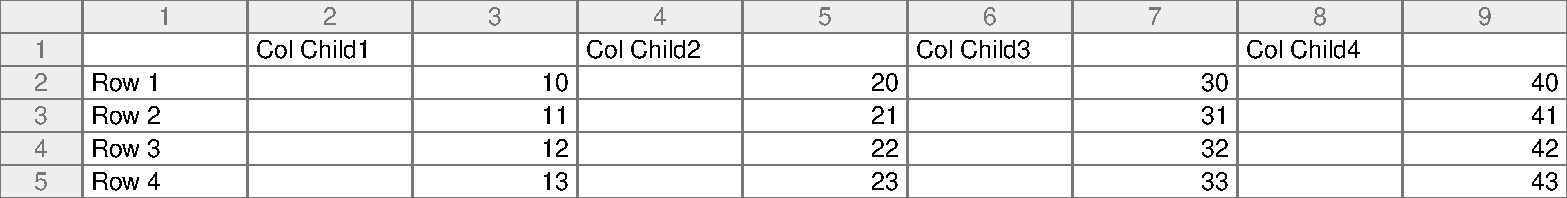
\includegraphics[width=\textwidth]{./TestCase/ToyExMismatchedColumnLabel.pdf}
\end{figure}
\begin{verbatim}
> rowData 
[1] 2 5
> colData 
[1] 3 9
> rowslist 
$label
[1] 1

$data
[1] 2 3 4 5

> colslist 
$label
[1] 1 2

$data
[1] 3 4 5 6 7 8 9

> plist 
$rows
[1] 1 2 3 4

$cols
[1] 1

> res 
Row 1 Row 2 Row 3 Row 4 
    1     2     3     4 
> rowplist 
Row 1 Row 2 Row 3 Row 4 
    1     2     3     4 
> rowvecs 
     [,1]   
[1,] "Row 1"
[2,] "Row 2"
[3,] "Row 3"
[4,] "Row 4"
> matColLabel 
     V2           V4           V6           V8          
[1,] "Col Child1" "Col Child2" "Col Child3" "Col Child4"
> cursub 
          V2           V4           V6           V8 
"Col Child1" "Col Child2" "Col Child3" "Col Child4" 
> currow[curcols] 
          V2           V4           V6           V8 
"Col Child1" "Col Child2" "Col Child3" "Col Child4" 
> matColLabel 
     V2           V4           V6           V8          
[1,] "Col Child1" "Col Child2" "Col Child3" "Col Child4"
> matColLabel 
     V2           V4           V6           V8          
[1,] "Col Child1" "Col Child2" "Col Child3" "Col Child4"
> matColLabel 
     V2           V4           V6           V8          
[1,] "Col Child1" "Col Child2" "Col Child3" "Col Child4"
> plist 
$rows
[1] 1 2 3 4

$cols
[1] 1

> res 
Col Child1 Col Child2 Col Child3 Col Child4 
         1          2          3          4 
> plist 
Col Child1 Col Child2 Col Child3 Col Child4 
         1          2          3          4 
> matData 
     V3   V5   V7   V9  
[1,] "10" "20" "30" "40"
[2,] "11" "21" "31" "41"
[3,] "12" "22" "32" "42"
[4,] "13" "23" "33" "43"
> datbit 
     V3   V5   V7   V9  
[1,] "10" "20" "30" "40"
[2,] "11" "21" "31" "41"
[3,] "12" "22" "32" "42"
[4,] "13" "23" "33" "43"
> colplist 
Col Child1 Col Child2 Col Child3 Col Child4 
         1          2          3          4 
> res 
  UNKNOWN Col Child1 Col Child2 Col Child3 Col Child4
1   Row 1         10         20         30         40
2   Row 2         11         21         31         41
3   Row 3         12         22         32         42
4   Row 4         13         23         33         43
\end{verbatim}

\newpage
\subsection{ToyExMultiRowColumnLabel.csv}
\label{sec:TCRO_ToyExMultiRowColumnLabel.csv}
\begin{figure}[!h]
\centering
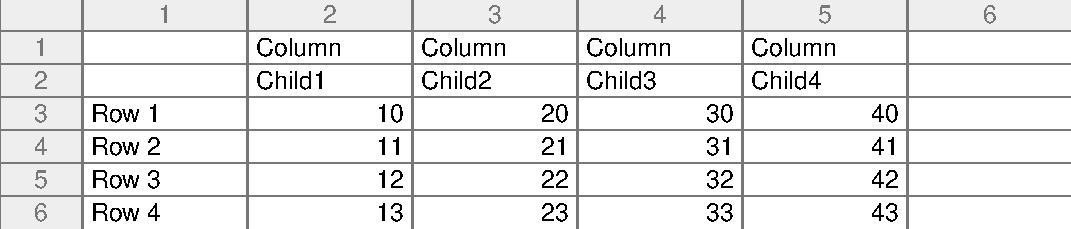
\includegraphics[width=\textwidth]{./TestCase/ToyExMultiRowColumnLabel.pdf}
\end{figure}
\begin{verbatim}
> rowData 
[1] 3 6
> colData 
[1] 2 5
> rowslist 
$label
[1] 1 2

$data
[1] 3 4 5 6

> colslist 
$label
[1] 1

$data
[1] 2 3 4 5

> plist 
$rows
[1] 1 2 3 4

$cols
[1] 1

> res 
Row 1 Row 2 Row 3 Row 4 
    1     2     3     4 
> rowplist 
Row 1 Row 2 Row 3 Row 4 
    1     2     3     4 
> rowvecs 
     [,1]   
[1,] "Row 1"
[2,] "Row 2"
[3,] "Row 3"
[4,] "Row 4"
> matColLabel 
     V2       V3       V4       V5      
[1,] "Column" "Column" "Column" "Column"
[2,] "Child1" "Child2" "Child3" "Child4"
> cursub 
      V2 
"Column" 
> currow[curcols] 
      V2 
"Column" 
> cursub 
      V3 
"Column" 
> currow[curcols] 
      V3 
"Column" 
> cursub 
      V4 
"Column" 
> currow[curcols] 
      V4 
"Column" 
> cursub 
      V5 
"Column" 
> currow[curcols] 
      V5 
"Column" 
> cursub 
      V2       V3       V4       V5 
"Child1" "Child2" "Child3" "Child4" 
> currow[curcols] 
      V2       V3       V4       V5 
"Child1" "Child2" "Child3" "Child4" 
> matColLabel 
     V2       V3       V4       V5      
[1,] "Column" "Column" "Column" "Column"
[2,] "Child1" "Child2" "Child3" "Child4"
> matColLabel 
     V2       V3       V4       V5      
[1,] "Column" "Column" "Column" "Column"
[2,] "Child1" "Child2" "Child3" "Child4"
> matColLabel 
     V2              V3              V4              V5             
[1,] "Column Child1" "Column Child2" "Column Child3" "Column Child4"
> plist 
$rows
[1] 1 2 3 4

$cols
[1] 1

> res 
Column Child1 Column Child2 Column Child3 Column Child4 
            1             2             3             4 
> plist 
Column Child1 Column Child2 Column Child3 Column Child4 
            1             2             3             4 
> matData 
     V2   V3   V4   V5  
[1,] "10" "20" "30" "40"
[2,] "11" "21" "31" "41"
[3,] "12" "22" "32" "42"
[4,] "13" "23" "33" "43"
> datbit 
     V2   V3   V4   V5  
[1,] "10" "20" "30" "40"
[2,] "11" "21" "31" "41"
[3,] "12" "22" "32" "42"
[4,] "13" "23" "33" "43"
> colplist 
Column Child1 Column Child2 Column Child3 Column Child4 
            1             2             3             4 
> res 
  UNKNOWN Column Child1 Column Child2 Column Child3 Column Child4
1   Row 1            10            20            30            40
2   Row 2            11            21            31            41
3   Row 3            12            22            32            42
4   Row 4            13            23            33            43
\end{verbatim}

\end{document}
\nwenddocs{}
